%\documentclass[twoside,10pt]{report}
\documentclass[10pt]{report}

% Package useful for debuging
%\usepackage{showlabels}

\usepackage{makeidx}
\usepackage{xtab}
\usepackage{amsmath, amssymb}

% Package to add Bibliography and Index to TOC
% but not the TOC itself :-)
\usepackage[nottoc]{tocbibind}

\usepackage{calc}

% Packages for adding figures
\usepackage{subfigure}
\usepackage{color}
\usepackage{graphicx}

% Needed for sideways
\usepackage{rotating}

% Packages used for output and source code listings
\usepackage{fancyvrb}
\usepackage{listings}

%\usepackage{fancyheadings}
\usepackage{fancyhdr}

% External references
\usepackage{xr}

% show margin lines for debugging
%\usepackage[showframe]{geometry}

%----- Define some colors
\definecolor{gray}{rgb}{0.5,0.5,0.5}

%----- Define the warning sign

\newcommand{\marginlabel}[1]
{\mbox{}\marginpar{\raggedleft\hspace{0pt}{\rule{0mm}{1mm}#1}}}

\newcommand{\warn}{%
%\marginlabel{\pstribox[shadow=false,fillstyle=solid,fillcolor=yellow,trimode=*U]{\footnotesize !}}%%
\marginlabel{
\includegraphics[scale=0.8]{warning}}%%
}

%----- Page formatting

\setlength{\paperwidth}{8.5in}
\setlength{\textwidth}{6.1in}
\setlength{\hoffset}{0.0in}
\setlength{\oddsidemargin}{0.2in}
\setlength{\evensidemargin}{0.2in}
\setlength{\marginparsep}{0.25in}
\setlength{\marginparwidth}{0.5in}

\setlength{\paperheight}{11.0in}
\setlength{\textheight}{9.0in}
\setlength{\voffset}{-0.25in}
\setlength{\topmargin}{0.0in}

%----- VERSIONS AND UCRL NUMBERS OF SUNDIALS CODES

\newcommand{\sunrelease}{v6.1.1}

\newcommand{\cvrelease}{v6.1.1}
\newcommand{\cvucrlug}{UCRL-SM-208108}
\newcommand{\cvucrlex}{UCRL-SM-208110}

\newcommand{\cvsrelease}{v6.1.1}
\newcommand{\cvsucrlug}{UCRL-SM-208111}
\newcommand{\cvsucrlex}{UCRL-SM-208115}

\newcommand{\idarelease}{v6.1.1}
\newcommand{\idaucrlug}{UCRL-SM-208112}
\newcommand{\idaucrlex}{UCRL-SM-208113}

\newcommand{\idasrelease}{v5.1.1}
\newcommand{\idasucrlug}{UCRL-SM-234051}
\newcommand{\idasucrlex}{LLNL-TR-437091}

\newcommand{\kinrelease}{v6.1.1}
\newcommand{\kinucrlug}{UCRL-SM-208116}
\newcommand{\kinucrlex}{UCRL-SM-208114}

\newcommand{\arkrelease}{v5.1.1}
\newcommand{\arkucrlug}{LLNL-SM-668082}
\newcommand{\arkucrlex}{????-??-??????}

%----- SUNDIALS MODULES
\newcommand{\sundials}{{\normalfont\scshape sundials}}
\newcommand{\shared}{{\normalfont\scshape shared}}
%----- Vectors:
\newcommand{\nvector}{{\normalfont\scshape nvector}}
\newcommand{\fnvector}{{\normalfont\scshape fnvector}}
\newcommand{\nvecs}{{\normalfont\scshape nvector\_serial}}
\newcommand{\nvecp}{{\normalfont\scshape nvector\_parallel}}
\newcommand{\nvecopenmp}{{\normalfont\scshape nvector\_openmp}}
\newcommand{\nvecopenmpdev}{{\normalfont\scshape nvector\_openmpdev}}
\newcommand{\nvecpthreads}{{\normalfont\scshape nvector\_pthreads}}
\newcommand{\nvecph}{{\normalfont\scshape nvector\_parhyp}}
\newcommand{\nvecpetsc}{{\normalfont\scshape nvector\_petsc}}
\newcommand{\nveccuda}{{\normalfont\scshape nvector\_cuda}}
\newcommand{\nvechip}{{\normalfont\scshape nvector\_hip}}
\newcommand{\nvecraja}{{\normalfont\scshape nvector\_raja}}
\newcommand{\nvecsycl}{{\normalfont\scshape nvector\_sycl}}
\newcommand{\nvectrilinos}{{\normalfont\scshape nvector\_trilinos}}
\newcommand{\nvecwrap}{{\normalfont\scshape nvector\_senswrapper}}
\newcommand{\nvecmanyvector}{{\normalfont\scshape nvector\_manyvector}}
\newcommand{\nvecmpimanyvector}{{\normalfont\scshape nvector\_mpimanyvector}}
\newcommand{\nvecmpiplusx}{{\normalfont\scshape nvector\_mpiplusx}}
%----- Matrices:
\newcommand{\sunmatrix}{{\normalfont\scshape sunmatrix}}
\newcommand{\fsunmatrix}{{\normalfont\scshape fsunmatrix}}
\newcommand{\sunmatband}{{\normalfont\scshape sunmatrix\_band}}
\newcommand{\sunmatdense}{{\normalfont\scshape sunmatrix\_dense}}
\newcommand{\sunmatsparse}{{\normalfont\scshape sunmatrix\_sparse}}
\newcommand{\sunmatcusparse}{{\normalfont\scshape sunmatrix\_cusparse}}
\newcommand{\sunmatslunrloc}{{\normalfont\scshape sunmatrix\_slunrloc}}
%----- Linear Solvers:
\newcommand{\sunlinsol}{{\normalfont\scshape sunlinsol}}
\newcommand{\fsunlinsol}{{\normalfont\scshape fsunlinsol}}
\newcommand{\sunlinsolband}{{\normalfont\scshape sunlinsol\_band}}
\newcommand{\sunlinsoldense}{{\normalfont\scshape sunlinsol\_dense}}
\newcommand{\sunlinsollapband}{{\normalfont\scshape sunlinsol\_lapackband}}
\newcommand{\sunlinsollapdense}{{\normalfont\scshape sunlinsol\_lapackdense}}
\newcommand{\sunlinsolklu}{{\normalfont\scshape sunlinsol\_klu}}
\newcommand{\sunlinsolsludist}{{\normalfont\scshape sunlinsol\_superludist}}
\newcommand{\sunlinsolslumt}{{\normalfont\scshape sunlinsol\_superlumt}}
\newcommand{\sunlinsolcuspbqr}{{\normalfont\scshape sunlinsol\_cusolversp\_batchqr}}
\newcommand{\sunlinsolspgmr}{{\normalfont\scshape sunlinsol\_spgmr}}
\newcommand{\sunlinsolspfgmr}{{\normalfont\scshape sunlinsol\_spfgmr}}
\newcommand{\sunlinsolspbcgs}{{\normalfont\scshape sunlinsol\_spbcgs}}
\newcommand{\sunlinsolsptfqmr}{{\normalfont\scshape sunlinsol\_sptfqmr}}
\newcommand{\sunlinsolpcg}{{\normalfont\scshape sunlinsol\_pcg}}
\newcommand{\sunlinsolcusparse}{{\normalfont\scshape sunlinsol\_cusparse}}
%----- Nonlinear Solvers:
\newcommand{\sunnonlinsol}{{\normalfont\scshape sunnonlinsol}}
\newcommand{\fsunnonlinsol}{{\normalfont\scshape fsunnonlinsol}}
\newcommand{\sunnonlinsolnewton}{{\normalfont\scshape sunnonlinsol\_newton}}
\newcommand{\sunnonlinsolfixedpoint}{{\normalfont\scshape sunnonlinsol\_fixedpoint}}
\newcommand{\sunnonlinsolpetsc}{{\normalfont\scshape sunnonlinsol\_petscsnes}}
%----- SUNMemory:
\newcommand{\sunmemory}{{\normalfont\scshape sunmemory}}
%----- Packages:
\newcommand{\cvode}{{\normalfont\scshape cvode}}
\newcommand{\pvode}{{\normalfont\scshape pvode}}
\newcommand{\cvodes}{{\normalfont\scshape cvodes}}
\newcommand{\arkode}{{\normalfont\scshape arkode}}
\newcommand{\ida}{{\normalfont\scshape ida}}
\newcommand{\idas}{{\normalfont\scshape idas}}
\newcommand{\kinsol}{{\normalfont\scshape kinsol}}
\newcommand{\sundialsTB}{{\normalfont\scshape sundialsTB}}

%----- OTHER PACKAGES
\newcommand{\vode}{{\normalfont\scshape vode}}
\newcommand{\vodpk}{{\normalfont\scshape vodpk}}
\newcommand{\lsode}{{\normalfont\scshape lsode}}
\newcommand{\daspk}{{\normalfont\scshape daspk}}
\newcommand{\daspkadjoint}{{\normalfont\scshape daspkadjoint}}
\newcommand{\hypre}{\textsl{hypre}}
\newcommand{\openmp}{{\normalfont OpenMP}}
\newcommand{\petsc}{{\normalfont\scshape pets}c}
\newcommand{\cuda}{{\normalfont\scshape cuda}}
\newcommand{\hip}{{\normalfont\scshape hip}}
\newcommand{\raja}{{\normalfont\scshape raja}}
\newcommand{\sycl}{{\normalfont\scshape sycl}}
\newcommand{\superludist}{SuperLU\_DIST}
\newcommand{\trilinos}{Trilinos}
\newcommand{\tpetra}{Tpetra}

%----- CVODE and CVODES COMPONENTS
\newcommand{\cvnls}{{\normalfont\scshape cvnls}}
\newcommand{\cvdls}{{\normalfont\scshape cvdls}}
\newcommand{\cvsls}{{\normalfont\scshape cvsls}}
\newcommand{\cvcls}{{\normalfont\scshape cvcls}}
\newcommand{\cvls}{{\normalfont\scshape cvls}}
\newcommand{\cvdense}{{\normalfont\scshape cvdense}}
\newcommand{\cvsparse}{{\normalfont\scshape cvsparse}}
\newcommand{\cvband}{{\normalfont\scshape cvband}}
\newcommand{\cvdiag}{{\normalfont\scshape cvdiag}}
\newcommand{\cvspils}{{\normalfont\scshape cvspils}}
\newcommand{\cvspgmr}{{\normalfont\scshape cvspgmr}}
\newcommand{\cvspbcg}{{\normalfont\scshape cvspbcg}}
\newcommand{\cvsptfqmr}{{\normalfont\scshape cvsptfqmr}}
\newcommand{\cvklu}{{\normalfont\scshape cvklu}}
\newcommand{\cvsuperlumt}{{\normalfont\scshape cvsuperlumt}}
\newcommand{\cvbandpre}{{\normalfont\scshape cvbandpre}}
\newcommand{\cvbbdpre}{{\normalfont\scshape cvbbdpre}}
\newcommand{\cvodea}{{\normalfont\scshape cvodea}}
\newcommand{\fcvode}{{\normalfont\scshape fcvode}}
\newcommand{\fcvbp}{{\normalfont\scshape fcvbp}}
\newcommand{\fcvbbd}{{\normalfont\scshape fcvbbd}}
\newcommand{\fcvroot}{{\normalfont\scshape fcvroot}}
\newcommand{\stald}{{\normalfont\scshape stald}}

%----- KINSOL COMPONENTS
\newcommand{\kinspils}{{\normalfont\scshape kinspils}}
\newcommand{\kinspgmr}{{\normalfont\scshape kinspgmr}}
\newcommand{\kinspfgmr}{{\normalfont\scshape kinspfgmr}}
\newcommand{\kinspbcg}{{\normalfont\scshape kinspbcg}}
\newcommand{\kinsptfqmr}{{\normalfont\scshape kinsptfqmr}}
\newcommand{\kinbbdpre}{{\normalfont\scshape kinbbdpre}}
\newcommand{\kindls}{{\normalfont\scshape kindls}}
\newcommand{\kincls}{{\normalfont\scshape kincls}}
\newcommand{\kinsls}{{\normalfont\scshape kinsls}}
\newcommand{\kinls}{{\normalfont\scshape kinls}}
\newcommand{\kindense}{{\normalfont\scshape kindense}}
\newcommand{\kinband}{{\normalfont\scshape kinband}}
\newcommand{\kinsparse}{{\normalfont\scshape kinsparse}}
\newcommand{\kinklu}{{\normalfont\scshape kinklu}}
\newcommand{\kinsuperlumt}{{\normalfont\scshape kinsuperlumt}}
\newcommand{\fkinbbd}{{\normalfont\scshape fkinbbd}}
\newcommand{\fkindense}{{\normalfont\scshape fkindense}}
\newcommand{\fkinband}{{\normalfont\scshape fkinband}}
\newcommand{\fkinsol}{{\normalfont\scshape fkinsol}}

%----- IDA and IDAS COMPONENTS
\newcommand{\idanls}{{\normalfont\scshape idanls}}
\newcommand{\idadls}{{\normalfont\scshape idadls}}
\newcommand{\idacls}{{\normalfont\scshape idacls}}
\newcommand{\idasls}{{\normalfont\scshape idasls}}
\newcommand{\idals}{{\normalfont\scshape idals}}
\newcommand{\idadense}{{\normalfont\scshape idadense}}
\newcommand{\idasparse}{{\normalfont\scshape idasparse}}
\newcommand{\idaband}{{\normalfont\scshape idaband}}
\newcommand{\idaklu}{{\normalfont\scshape idaklu}}
\newcommand{\idasuperlumt}{{\normalfont\scshape idasuperlumt}}
\newcommand{\idaspils}{{\normalfont\scshape idaspils}}
\newcommand{\idaspgmr}{{\normalfont\scshape idaspgmr}}
\newcommand{\idaspbcg}{{\normalfont\scshape idaspbcg}}
\newcommand{\idasptfqmr}{{\normalfont\scshape idasptfqmr}}
\newcommand{\idabbdpre}{{\normalfont\scshape idabbdpre}}
\newcommand{\idaa}{{\normalfont\scshape idaa}}
\newcommand{\fida}{{\normalfont\scshape fida}}
\newcommand{\fidaband}{{\normalfont\scshape fidaband}}
\newcommand{\fidadense}{{\normalfont\scshape fidadense}}
\newcommand{\fidabbd}{{\normalfont\scshape fidabbd}}
\newcommand{\fidaroot}{{\normalfont\scshape fidaroot}}

%----- SHARED COMPONENTS
\newcommand{\sundialsmath}{{\normalfont\scshape sundialsmath}}
\newcommand{\diag}{{\normalfont\scshape diag}}
\newcommand{\dense}{{\normalfont\scshape dense}}
\newcommand{\band}{{\normalfont\scshape band}}
\newcommand{\pcg}{{\normalfont\scshape pcg}}
\newcommand{\sls}{{\normalfont\scshape sls}}
\newcommand{\sparse}{{\normalfont\scshape sparse}}
\newcommand{\spgmr}{{\normalfont\scshape spgmr}}
\newcommand{\spfgmr}{{\normalfont\scshape spfgmr}}
\newcommand{\spbcg}{{\normalfont\scshape spbcgs}}
\newcommand{\spbcgs}{{\normalfont\scshape spbcgs}}
\newcommand{\sptfqmr}{{\normalfont\scshape sptfqmr}}
\newcommand{\klu}{{\normalfont\scshape klu}}
\newcommand{\superlumt}{{\normalfont\scshape superlumt}}

%----- OS
\newcommand{\linux}{{\sc LINUX}}
\newcommand{\unix}{{\sc UNIX}}
\newcommand{\mpi}{{\sc MPI}}

%----- C and Fortran languages
\newcommand{\CC}{{\sc C}}
\newcommand{\CPP}{{\sc C}\raisebox{0.2em}{\tiny ++}}
\newcommand{\F}{{\sc Fortran}}

%------ Serial, OpenMP, Pthreads, Parallel, or ParHyp
\newcommand{\s}{[{\bf S}]}
\newcommand{\omp}{[{\bf O}]}
\newcommand{\pt}{[{\bf T}]}
\newcommand{\p}{[{\bf P}]}
\newcommand{\h}{[{\bf H}]}

%------ Appendix in text
\newcommand{\A}{App. }

%------ Index entries

\newcommand{\ID}[1]{{\tt #1}{\index{#1@\texttt{#1}}}}
%\newcommand{\ID}[1]{{\tt #1}{\index{#1@\texttt{#1}|textbf}}}
% NOTE: the above version confuses hyperref...
\newcommand{\Id}[1]{{\tt #1}{\index{#1@\texttt{#1}}}}
\newcommand{\id}[1]{{\tt #1}}

%%----- Shortcuts for math formulas
\newcommand{\mb}[1]{{\mbox{\scriptsize #1}}}

\newcommand{\dfdy}{\frac{\partial f}{\partial y}}
\newcommand{\dfdyI}{\partial f / \partial y}
\newcommand{\dfdpi}{\frac{\partial f}{\partial p_i}}
\newcommand{\dfdpiI}{\partial f / \partial p_i}

\newcommand{\dFdy}{\frac{\partial F}{\partial y}}
\newcommand{\dFdyI}{\partial F / \partial y}
\newcommand{\dFdyp}{\frac{\partial F}{\partial \dot y}}
\newcommand{\dFdypI}{\partial F / \partial \dot y}
\newcommand{\dFdpi}{\frac{\partial F}{\partial p_i}}
\newcommand{\dFdpiI}{\partial F / \partial p_i}

\newcommand{\rhomax}{\rho_{\max}}

\newcommand{\cm}{$\checkmark$}

\newcommand{\newlinefill}[1]{\newline\phantom{#1}}

%%------ Specify depths for section numbering and TOC

\setcounter{tocdepth}{1}
\setcounter{secnumdepth}{3}

%%-------

\newcommand{\includeCode}[1]
{
  \VerbatimInput[numbers=left,fontsize=\small]{#1}
}

\newcommand{\includeOutput}[2]
{
  \vspace{0.1in}
  \VerbatimInput[frame=single,
                 framesep=0.1in,
                 label={\tt #1} sample output,
                 fontsize=\footnotesize]{#2}
}

%%-------

\newcommand{\ugref}[1]{\S\ref{#1}}

%%-------

\newcommand{\clearemptydoublepage}{\newpage{\pagestyle{empty}\cleardoublepage}}

%%-------

\newcommand{\disclaimer}{%
\thispagestyle{empty}% no number of this page
\vglue5\baselineskip
\begin{center}
{\bf DISCLAIMER}
\end{center}
\noindent
This document was prepared as an account of work sponsored by an agency of
the United States government. Neither the United States government nor
Lawrence Livermore National Security, LLC, nor any of their employees makes
any warranty, expressed or implied, or assumes any legal liability or responsibility
for the accuracy, completeness, or usefulness of any information, apparatus, product,
or process disclosed, or represents that its use would not infringe privately owned rights.
Reference herein to any specific commercial product, process, or service by trade name,
trademark, manufacturer, or otherwise does not necessarily constitute or imply its endorsement,
recommendation, or favoring by the United States government or Lawrence Livermore National
Security, LLC. The views and opinions of authors expressed herein do not necessarily state
or reflect those of the United States government or Lawrence Livermore National Security, LLC,
and shall not be used for advertising or product endorsement purposes.

\vskip2\baselineskip
\noindent This work was performed under the auspices of the U.S. Department of Energy by Lawrence
Livermore National Laboratory under Contract DE-AC52-07NA27344.
\vfill
\begin{center}
Approved for public release; further dissemination unlimited
\end{center}
\clearpage
}

%%-------

\newcommand{\contributors}{%
\thispagestyle{empty}% no number of this page
\vglue5\baselineskip
\begin{center}
{\bf CONTRIBUTORS}
\end{center}
\noindent
The SUNDIALS library has been developed over many years by a number of
contributors. The current SUNDIALS team consists of Cody J. Balos,
David J. Gardner, Alan C. Hindmarsh, Daniel R. Reynolds, and
Carol S. Woodward. We thank Radu Serban for significant and critical past
contributions.\\
\\
\noindent
Other contributors to SUNDIALS include: James Almgren-Bell, Lawrence E. Banks,
Peter N. Brown, George Byrne, Rujeko Chinomona, Scott D. Cohen, Aaron Collier,
Keith E. Grant, Steven L. Lee, Shelby L. Lockhart, John Loffeld, Daniel McGreer,
Slaven Peles, Cosmin Petra, H. Hunter Schwartz, Jean M. Sexton,
Dan Shumaker, Steve G. Smith, Allan G. Taylor, Hilari C. Tiedeman, Chris White,
Ting Yan, and Ulrike M. Yang.
\clearpage
}

%%--------------------------------

\newcommand{\frontug}
{

  %% Start roman numbering
  \pagenumbering{roman}

  %% Title page
  \maketitle
  \disclaimer
  \contributors
  \clearemptydoublepage

  %% Contents, tables, and figures
  \tableofcontents
  \clearemptydoublepage
  \listoftables
  \clearemptydoublepage
  \listoffigures
  \clearemptydoublepage

  %% Start arabic numbering
  \pagenumbering{arabic}

  %% Define page style for the body of the document
  \lhead[\fancyplain{}{\bfseries\thepage}]%
        {\fancyplain{}{\bfseries\rightmark}}
  \rhead[\fancyplain{}{\bfseries\leftmark}]%
        {\fancyplain{}{\bfseries\thepage}}
  \cfoot{}
  \pagestyle{fancyplain}


  %% Some settings for code listings
  \lstset{
    language=C, fancyvrb=true,
    basicstyle=\footnotesize\ttfamily,
    commentstyle=\color{MidnightBlue},
    keywordstyle=\color{BrickRed},
    stringstyle=\color{OliveGreen},
    numbers=left, numberstyle=\tiny, numbersep=15pt}

}

%%--------------------------------
\newcommand{\frontex}
{

  \pagestyle{empty}
  \maketitle
  \disclaimer
  \contributors
  \clearemptydoublepage

  % Contents
  \tableofcontents

  %% Start arabic numbering
  \clearemptydoublepage
  %%\clearpage
  \pagestyle{plain}\pagenumbering{arabic}

  %% Some settings for code listings
  \lstset{
    fancyvrb=true,
    basicstyle=\footnotesize\ttfamily,
    commentstyle=\color{MidnightBlue},
    keywordstyle=\color{BrickRed},
    stringstyle=\color{OliveGreen},
    numbers=left, numberstyle=\tiny, numbersep=15pt}

}

%%----------------------------------
%% List of configure options
%%---------------------------------
\newenvironment{config}
{\begin{list}{}{
      \setlength{\leftmargin}{2em}
      \setlength{\rightmargin}{0em}
      \setlength{\topsep}{0.05in}
      \setlength{\itemindent}{-2em}
      \setlength{\itemsep}{0.05in}}}
  {\end{list}}
%%---------------------------------
%% Steps used in skeleton programs
%%---------------------------------
\newcounter{Stepsctr}
\newenvironment{Steps}
{\stepcounter{Stepsctr}
  \begin{list}{\arabic{Stepsctr}. }{
      \usecounter{Stepsctr}
      \setlength{\parsep}{0.5em}
      \setlength{\labelsep}{0em}
      \settowidth{\labelwidth}{99. }
      \setlength{\leftmargin}{\labelwidth+\labelsep}}}
  {\end{list}}
%%-----------------------------------------------------
%% Underlying list environemnt for function definitions
%%-----------------------------------------------------
\newenvironment{Ventry}[1][\quad]
{\begin{list}{}{
      \setlength{\rightmargin}{0em}
      \setlength{\topsep}{0.05in}
      \setlength{\itemsep}{0em}
      \setlength{\itemindent}{0em}
      \setlength{\labelsep}{0.5em}
      \renewcommand{\makelabel}[1]{##1\hfill}
      \settowidth{\labelwidth}{#1}
      \setlength{\leftmargin}{\labelwidth+\labelsep}}}
  {\end{list}}
%%----------------------------------
%% List of function arguments
%%---------------------------------
\newenvironment{args}[1][\quad]
{\begin{list}{}{
      \setlength{\rightmargin}{0em}
      \setlength{\topsep}{0em}
      \setlength{\itemsep}{0em}
      \setlength{\itemindent}{0em}
      \setlength{\labelsep}{0.5em}
      \renewcommand{\makelabel}[1]{\id{##1}\hfill}
      \settowidth{\labelwidth}{\id{#1}}
      \setlength{\leftmargin}{\labelwidth+\labelsep}}}
  {\end{list}}
%%---------------------------------
%% User-callable function
%%---------------------------------
\newcommand{\ucfunction}[6]{
  \noindent\paragraph{\fbox{\id{#1}}}
  \begin{Ventry}[Return value]
  \item[Call]{\id{#2}}
  \item[Description]{#3}
  \addArgs{#4}
  \addRetval{#5}
  \addNotes{#6}
  \end{Ventry}
}
%%----------------------------------------------
%% User-callable function with a deprecated name
%%----------------------------------------------
\newcommand{\ucfunctiond}[7]{
  \noindent\paragraph{\fbox{\id{#1}}}
  \begin{Ventry}[Deprecated Name]
  \item[Call]{\id{#2}}
  \item[Description]{#3}
  \addArgs{#4}
  \addRetval{#5}
  \addNotes{#6}
  \addDepName{#7}
  \end{Ventry}
}
%%-----------------------------------------------------
%% User-callable function with a Fortran 2003 interface
%%-----------------------------------------------------
\newcommand{\ucfunctionf}[6]{
  \noindent\paragraph{\fbox{\id{#1}}}
  \begin{Ventry}[Return value]
  \item[Call]{\id{\begin{tabular}[t]{@{}r@{}l@{}}#2\end{tabular}}}
  \item[Description]{#3}
  \addArgs{#4}
  \addRetval{#5}
  \addNotes{#6}
  \item[F2003 Name]{\id{F#1}}
  \end{Ventry}
}
%%-----------------------------------------------------
%% User-callable function with a Fortran 2003 interface
%% and an additional entry on how to call the F2003
%% function.
%%-----------------------------------------------------
\newcommand{\ucfunctionfl}[7]{
  \noindent\paragraph{\fbox{\id{#1}}}
  \begin{Ventry}[Return value]
  \item[Call]{\id{#2}}
  \item[Description]{#3}
  \addArgs{#4}
  \addRetval{#5}
  \addNotes{#6}
  \item[F2003 Name]{\id{F#1}}
  \item[F2003 Call]{\id{#7}}
  \end{Ventry}
}
%%-----------------------------------------------------
%% User-callable function with a deprecated name and
%% a Fortran 2003 interface
%%-----------------------------------------------------
\newcommand{\ucfunctiondf}[7]{
  \noindent\paragraph{\fbox{\id{#1}}}
  \begin{Ventry}[Deprecated Name]
  \item[Call]{\id{#2}}
  \item[Description]{#3}
  \addArgs{#4}
  \addRetval{#5}
  \addNotes{#6}
  \addDepName{#7}
  \item[F2003 Name]{\id{F#1}}
  \end{Ventry}
}
%%--------------------------------------------
%% macro for generic SUNDIALS module functions
%%--------------------------------------------
\newcommand{\sunmodfun}[3]{
  \noindent\paragraph{\fbox{\ID{#1}}}
  \begin{Ventry}[F2003 Name]
  \item[Prototype]{\id{#3}}
  \item[Description]{#2}
  \end{Ventry}
}
%%-------------------------------------------------------
%% macro for generic overloaded SUNDIALS module functions
%%-------------------------------------------------------
\newcommand{\sunmodfuns}[6]{
  \noindent\paragraph{\fbox{\ID{#1}}}
  \begin{Ventry}[F2003 Name]
  \item[\textit{Single-node usage}]{}
  \item[Prototype]{\id{#4}}
  \item[Description]{#2#3}
  \item[\textit{Distributed-memory parallel usage}]{}
  \item[Prototype]{\id{#6}}
  \item[Description]{#2#5}
  \end{Ventry}
}
%%--------------------------------------------------------------------------
%% macro for generic SUNDIALS module functions with a Fortran 2003 interface
%%--------------------------------------------------------------------------
\newcommand{\sunmodfunf}[3]{
  \noindent\paragraph{\fbox{\ID{#1}}}
  \begin{Ventry}[F2003 Name]
  \item[Prototype]{\id{#3}}
  \item[Description]{#2}
  \item[F2003 Name]{This function is callable as \id{F#1} when using the Fortran
  2003 interface module.}
  \end{Ventry}
}
%%---------------------------------
%% User-supplied function
%%---------------------------------
\newcommand{\usfunction}[6]{
  \noindent\paragraph{\fbox{\id{#1}}}
  \begin{Ventry}[Return value]
  \item[Definition]{\id{\begin{tabular}[t]{@{}r@{}l@{}}#2\end{tabular}}}
  \item[Purpose]{#3}
  \item[Arguments]{#4}
  \item[Return value]{#5}
  \addNotes{#6}
  \end{Ventry}
}
%%---------------------------------
\makeatletter
\long\def\addArgs#1{\def\@tempa{#1}\ifx\@tempa\empty\item[Arguments]{None}\else\item[Arguments]{#1}\fi}
\makeatother
%%---------------------------------
\makeatletter
\long\def\addRetval#1{\def\@tempa{#1}\ifx\@tempa\empty\item[Return value]{None}\else\item[Return value]{#1}\fi}
\makeatother
%%---------------------------------
\makeatletter
\long\def\addNotes#1{\def\@tempa{#1}\ifx\@tempa\empty\else\item[Notes]{#1}\fi}
\makeatother
%%---------------------------------
\makeatletter
\long\def\addDepName#1{\def\@tempa{#1}\ifx\@tempa\empty\item[Deprecated
  Name]{None}\else\item[Deprecated Name]{For backward compatibility, the wrapper
  function \id{#1} with idential input and output arguments is also
  provided.}\fi}
\makeatother


%%---------------------------------
%% Finally, use hyperref package to include links in the PDF
%% Note that since hyperref redefines a bunch of LaTeX commands,
%% to give it a fighting chance, it MUST be included last.

\usepackage[
% letterpaper=true,
% dvips,
% ps2pdf,
hyperindex=true,
linktocpage=true,
colorlinks=true,
linkcolor=blue,
citecolor=blue,
bookmarks=true]
{hyperref}


%===============================================================

\newcommand{\cvucrl}{UCRL-SM-208108}
\newcommand{\cvdate}{November 2004}
\newcommand{\cvrelease}{v2.2.0}

\title{User Documentation for {\cvode} {\cvrelease}}
\author{
  Alan C. Hindmarsh and Radu Serban\\
  {\em Center for Applied Scientific Computing} \\
  {\em Lawrence Livermore National Laboratory}
}
\date{}

%===============================================================

\makeindex

%===============================================================

\begin{document}

%Create the LLNL Cover Page
\makeLLNLCover{\cvucrl}%                           UCRL number
{User Documentation for CVODE {\cvrelease}}%    Title on cover page
{Alan C. Hindmarsh and Radu Serban}%               Authors
{\cvdate}%                                         Date
{0in}{0in}

\frontug
\renewcommand{\chaptermark}[1]{\markboth{#1}{}}
\renewcommand{\sectionmark}[1]{\markright{\thesection\ #1}}

%===============================================================
% Introduction
%===================================================================================
\chapter{Introduction}\label{s:intro}
%===================================================================================

{\cvode} is part of a software family called {\sundials}: 
SUite of Nonlinear and DIfferential/ALgebraic equation Solvers.  
This suite consists of {\cvode}, {\kinsol}, and {\ida}, and variants of these
with sensitivity analysis capabilities.
%
%---------------------------------
\section{Historical Background}\label{ss:history}
%---------------------------------

\index{CVODE@{\cvode}!relationship to {\vode}, {\vodpk}|(}
{\F} solvers for ODE initial value problems are widespread and heavily used. 
Two solvers that have been written at LLNL in the past are {\vode} \cite{BBH:89} 
and {\vodpk} \cite{Byr:92}.
{\vode}\index{VODE@{\vode}} is a general purpose solver that includes methods for stiff
and nonstiff systems, and in the stiff case uses direct methods (full or
banded) for the solution of the linear systems that arise at each implicit
step. Externally, {\vode} is very similar to the well known solver
{\lsode}\index{LSODE@{\lsode}} \cite{RaHi:94}.
{\vodpk}\index{VODPK@{\vodpk}} is a variant of {\vode} that uses a preconditioned Krylov 
(iterative) method for the solution of the linear systems. {\vodpk} is a powerful 
tool for large stiff systems because it combines established methods for stiff 
integration, nonlinear iteration, and Krylov (linear) iteration with a problem-specific
treatment of the dominant source of stiffness, in the form of the user-supplied
preconditioner matrix \cite{BrHi:89}.
The capabilities of both {\vode} and {\vodpk} have been combined in the {\C}-language 
package {\cvode}\index{CVODE@{\cvode}} \cite{CoHi:96}.

In the process of translating the {\vode} and {\vodpk} algorithms into {\C}, the overall 
{\cvode} organization has been changed considerably.
One key feature of the {\cvode} organization is that the linear system solvers comprise a
layer of code modules that is separated from the integration algorithm, allowing for 
easy modification and expansion of the linear solver array.
A second key feature is a separate module devoted to vector operations; this 
facilitated the extension to multiprosessor environments with minimal impacts 
on the rest of the solver, resulting in {\pvode}\index{PVODE@{\pvode}} \cite{ByHi:99}, 
the parallel variant of {\cvode}.
\index{CVODE@{\cvode}!relationship to {\vode}, {\vodpk}|)}

\index{CVODE@{\cvode}!relationship to {\cvode}, {\pvode}|(}
Recently, the functionality of {\cvode} and {\pvode} has been combined into
one single code, simply called {\cvode}.
Development of the new version of {\cvode} was concurrent with a redesign of the vector operations module
across the {\sundials} suite. The key feature of the new {\nvector} module is that it
is written in terms of abstract vector operations with the actual vector kernels attached
by a particular implementation (such as serial or parallel) of {\nvector}. This allows
writing the {\sundials} solvers in a manner independent of the actual {\nvector} 
implementation (which can be user-supplied), as well as allowing more than one 
{\nvector} module linked into an executable file.
\index{CVODE@{\cvode}!relationship to {\cvode}, {\pvode}|)}

\index{CVODE@{\cvode}!motivation for writing in C|(}
There are several motivations for choosing the {\C} language for {\cvode}.
First, a general movement away from {\F} and toward {\C} in scientific
computing is apparent.  Second, the pointer, structure, and dynamic
memory allocation features in C are extremely useful in software of
this complexity, with the great variety of method options offered.
Finally, we prefer {\C} over {\CPP} for {\cvode} because of the wider
availability of {\C} compilers, the potentially greater efficiency of {\C},
and the greater ease of interfacing the solver to applications written
in extended {\F}.
\index{CVODE@{\cvode}!motivation for writing in C|)}

\paragraph{Aknowledgments.}
We wish to aknowledge the contributions to previous versions of the
{\cvode} and {\pvode} codes and user guides of Scott D. Cohen \cite{CoHi:94}
and George D. Byrne \cite{ByHi:98}.

\section{Changes in version 2.1}
The major changes from the previous version involve a redesign of the
user interface across the entire {\sundials} suite. We have eliminated the
mechanism of providing optional inputs and extracting optional statistics 
from the solver through the \id{iopt} and \id{ropt} arrays. Instead,
{\cvode} now provides a set of routines (with prefix \id{CVodeSet})
to change the default values for various quantities controlling the
solver and a set of extraction routines (with prefix \id{CVodeGet})
to extract statistics after return from the main solver routine.
Similarly, each linear solver module provides its own set of {\id{Set}-}
and {\id{Get}-type} routines. For more details see \S\ref{ss:optional_input}
and \S\ref{ss:optional_output}.

Additionally, the interfaces to several user-supplied routines
(such as those providing Jacobians, preconditioner information, and
sensitivity right hand sides) were simplified by reducing the number
of arguments. The same information that was previously accessible
through such arguments can now be obtained through {\id{Get}-type}
functions.

Installation of {\cvodes} (and all of {\sundials}) has been completely 
redesigned and is now based on configure scripts.

\section{Reading this User Guide}\label{ss:reading}

This user guide is a combination of general usage instructions and
specific example programs.  We expect that some readers will want to
concentrate on the general instructions, while others will refer
mostly to the examples, and the organization is intended to
accommodate both styles.

There are different possible levels of usage of {\cvode}. The most casual
user, with a small IVP problem only, can get by with reading \S\ref{ss:ivp_sol}, 
then \S\ref{s:simulation} through \S\ref{sss:cvode} only, and looking at examples 
in \cite{cvode2.1_ex}. 
In a different direction, a more expert user with an IVP problem may want
to (a) use a package preconditioner (\S\ref{ss:preconds}), (b) supply
his/her own Jacobian or preconditioner routines (\S\ref{ss:user_fct_sim}),
(c) do multiple runs of problems of the same size (\S\ref{sss:cvreinit}), 
(d) supply a new {\nvector} module (\S\ref{s:nvector}), or even 
(e) supply a different linear solver module
(\S\ref{ss:cvode_org} and \S\ref{s:gen_linsolv}).

The structure of this document is as follows:
\begin{itemize}
\item
  In \S\ref{s:install} we begin with instructions for the installation of 
  {\cvode}, within the structure of {\sundials}.
\item
  In \S\ref{s:math}, we give short descriptions of the numerical 
  methods implemented by {\cvode} for the solution of initial value problems
  for systems of ODEs.
\item
  The following section describes the structure of the {\sundials} suite
  of solvers (\S\ref{ss:sun_org}) and the software organization of the {\cvode}
  solver (\S\ref{ss:cvode_org}). 
\item
  In \S\ref{s:simulation}, we give an overview of the usage of {\cvode},
  as well as a complete description of the user interface and of the 
  user-defined routines for integration of IVP ODEs.
\item
  Section \ref{s:nvector} gives a brief overview of the generic {\nvector} module 
  shared among the various components of {\sundials}, as well as details on the two {\nvector}
  implementations provided with {\sundials}: a serial implementation
  (\S\ref{ss:nvec_ser}) and a parallel implementation, based on MPI\index{MPI}
  (\S\ref{ss:nvec_par}).
\item
  Section \ref{s:gen_linsolv} describes in detail the generic linear solvers shared 
  by all {\sundials} solvers.
\end{itemize}

Finally, the reader should be aware of the following notational conventions
in this user guide:  program listings and identifiers (such as \id{CVodeMalloc}) 
within textual explanations appear in typewriter type style; 
fields in {\C} structures (such as {\em content}) appear in italics;
and packages or modules, such as {\cvdense}, are written in all capitals. 
In the Index, page numbers that appear in bold indicate the main reference
for that entry.
%===============================================================
% SUNDIALS installation procedure
\chapter{{\sundials} Installation Procedure}\label{s:install}
\chapter{SUNDIALS Package Installation Procedure}\label{c:install}

The installation of any {\sundials} package is accomplished by installing the
{\sundials} suite as a whole, according to the instructions that
follow. The same procedure applies whether or not the downloaded
file contains one or all solvers in {\sundials}.

The {\sundials} suite (or individual solvers) are distributed as
compressed archives (\id{.tar.gz}). The name of the distribution
archive is of the form {\em solver}\id{-x.y.z.tar.gz}, where {\em solver}
is one of: \id{sundials}, \id{cvode}, \id{cvodes}, \id{arkode}, \id{ida},
\id{idas}, or \id{kinsol}, and \id{x.y.z} represents the version number
(of the {\sundials} suite or of the individual solver).
%%
To begin the installation, first uncompress and expand the sources, by issuing
\begin{verbatim}
   % tar xzf solver-x.y.z.tar.gz
\end{verbatim}
This will extract source files under a directory {\em solver}\id{-x.y.z}.

Starting with version \id{2.6.0} of {\sundials}, CMake is the only supported method
of installation.
The explanations of the installation procedure begins with a few common observations:
%%
\begin{itemize}

\item The remainder of this chapter will follow these conventions:
  \begin{description}
  \item[{\em solverdir}] 
    is the directory {\em solver}\id{-x.y.z} created above; i.e., the 
    directory containing the {\sundials} sources.
  \item[{\em builddir}]
    is the (temporary) directory under which {\sundials} is built.
  \item[{\em instdir}]
    is the directory under which the {\sundials} exported header files
    and libraries will be installed. Typically, header files are exported under a directory
    {\em instdir}\id{/include} while libraries are installed under {\em instdir}\id{/lib},
    with {\em instdir} specified at configuration time.
  \end{description}

\item For {\sundials} CMake-based installation, in-source builds are prohibited; in other words, the
  build directory {\em builddir} can {\bf not} be the same as {\em solverdir}
  and such an attempt will lead to an error. This
  prevents ``polluting'' the source tree and allows efficient builds
  for different configurations and/or options.

\item {\warn}The installation directory {\em instdir} can {\bf not} be the same as
  the source directory {\em solverdir}.

\item By default, only the libraries and header files are exported to the installation
  directory {\em instdir}.  If enabled by the user (with the
  appropriate toggle for CMake), the
  examples distributed with {\sundials} will be built together with
  the solver libraries but the installation step will result in
  exporting (by default in a subdirectory of the installation
  directory) the example sources and sample outputs together with
  automatically generated configuration files that reference the {\em
  installed} {\sundials} headers and libraries.  As such, these
  configuration files for the {\sundials} examples can be used as
  ``templates'' for your own problems. CMake installs \id{CMakeLists.txt} files and also
  (as an option available only under Unix/Linux) \id{Makefile} files. Note this
  installation approach also allows the option of building the
  {\sundials} examples without having to install them.  (This can be
  used as a sanity check for the freshly built libraries.)

\item Even if generation of shared libraries is enabled, only static libraries
  are created for the FCMIX modules.  (Because of the use of fixed names for
  the Fortran user-provided subroutines, FCMIX shared libraries would result in
  ``undefined symbol'' errors at link time.)

\end{itemize}


%%===============================================================================
\section{CMake-based installation}\label{s:cmake_inst}
%%===============================================================================

CMake-based installation provides a platform-independent build system. CMake can generate
Unix and Linux Makefiles, as well as KDevelop, Visual Studio, and 
(Apple) XCode project files from the same configuration file.
In addition, CMake also provides a GUI front end and which allows an interactive build and
installation process.

The {\sundials} build process requires CMake version \id{3.0.2} or
higher and a working {\CC} compiler.  On Unix-like operating systems, it
also requires Make (and \id{curses}, including its development libraries,
for the GUI front end to CMake, \id{ccmake}), while on Windows it
requires Visual Studio.  While many Linux distributions offer CMake,
the version included may be out of date.  Many new CMake
features have been added recently, and you should download the latest
version from {\tt http://www.cmake.org}.  Build instructions for CMake
(only necessary for Unix-like systems) can be found on the CMake website.
Once CMake is installed, Linux/Unix users will be able to use \id{ccmake},
while Windows users will be able to use \id{CMakeSetup}.

As previously noted, when using CMake to configure, build and install {\sundials}, it is always
required to use a separate build directory. While in-source builds are possible, they are
explicitly prohibited by the {\sundials} CMake scripts (one of the reasons being that, unlike
autotools, CMake does not provide a \id{make distclean} procedure and it is therefore
difficult to clean-up the source tree after an in-source build). By ensuring a separate build
directory, it is an easy task for the user to clean-up all traces of the build by simply removing
the build directory. CMake does generate a \id{make clean} which will remove files generated by the
compiler and linker.

\subsection{Configuring, building, and installing on Unix-like systems}

The default CMake configuration will build all included solvers and
associated examples and will build static and shared libraries. The
{\em instdir} defaults to \id{/usr/local} and can be changed by
setting the \id{CMAKE\_INSTALL\_PREFIX} variable.  Support for FORTRAN
and all other options are disabled.

CMake can be used from the command line with the \id{cmake} command, or from a \id{curses}-based GUI
by using the \id{ccmake} command. Examples for using both methods will be presented.
For the examples shown it is assumed that there is a top level {\sundials} directory
with appropriate source, build and install directories:

\begin{verbatim}
   % mkdir (...)sundials/instdir
   % mkdir (...)sundials/builddir
   % cd (...)sundials/builddir
\end{verbatim}

%%
%% Building with the GUI configuration
%%
\subsubsection*{Building with the GUI}

Using CMake with the GUI follows this general process:  
\begin{itemize}
\item Select and modify values, run configure (\id{c} key)
\item New values are denoted with an asterisk
\item To set a variable, move the cursor to the variable and press enter
  \begin{itemize}
  \item If it is a boolean (ON/OFF) it will toggle the value
  \item If it is string or file, it will allow editing of the string
  \item For file and directories, the \id{<tab>} key can be used to complete 
  \end{itemize}
\item Repeat until all values are set as desired and the generate option is available (\id{g} key)
\item Some variables (advanced variables) are not visible right away
\item To see advanced variables, toggle to advanced mode (\id{t} key)
\item To search for a variable press \id{/} key, and to repeat the search, press the
\id{n} key
\end{itemize}

To build the default configuration using the GUI, from the {\em builddir} enter
the ccmake command and point to the {\em solverdir}:

\begin{verbatim}
    % ccmake ../solverdir
\end{verbatim}

The default configuration screen is shown in Figure
\ref{f:ccmakedefault}. 
\begin{figure}[!ht]
{\centerline{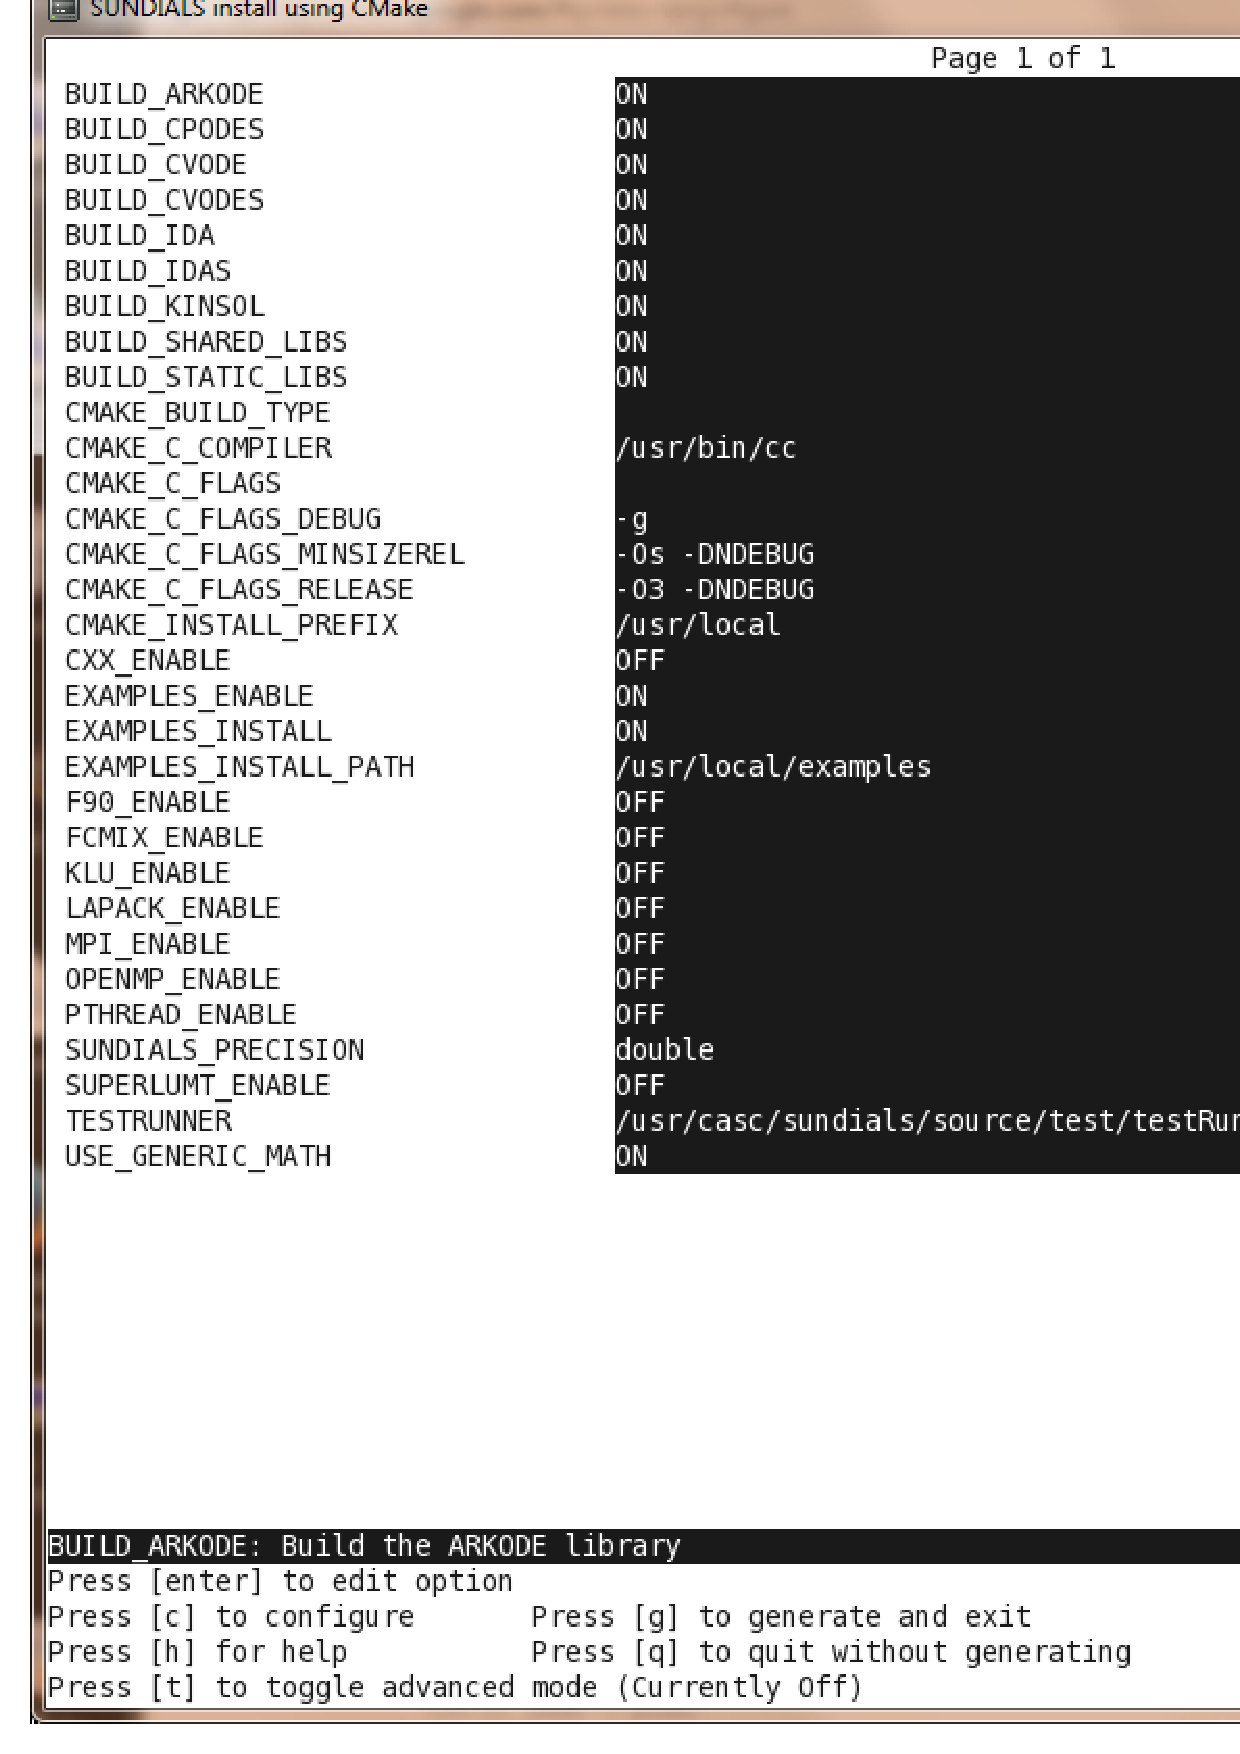
\includegraphics[width=\textwidth]{ccmakedefault}}}
\caption [Initial {\em ccmake} configuration screen]
{Default configuration screen. Note: Initial screen is empty.
To get this default configuration, press 'c' repeatedly (accepting default values denoted with asterisk)
until the 'g' option is available.}
\label{f:ccmakedefault}
\end{figure}

The default {\em instdir} for both {\sundials} and corresponding examples
can be changed by setting the \id{CMAKE\_INSTALL\_PREFIX} and
the \id{EXAMPLES\_INSTALL\_PATH} as shown in figure
\ref{f:ccmakeprefix}. 
\begin{figure}[!ht]
{\centerline{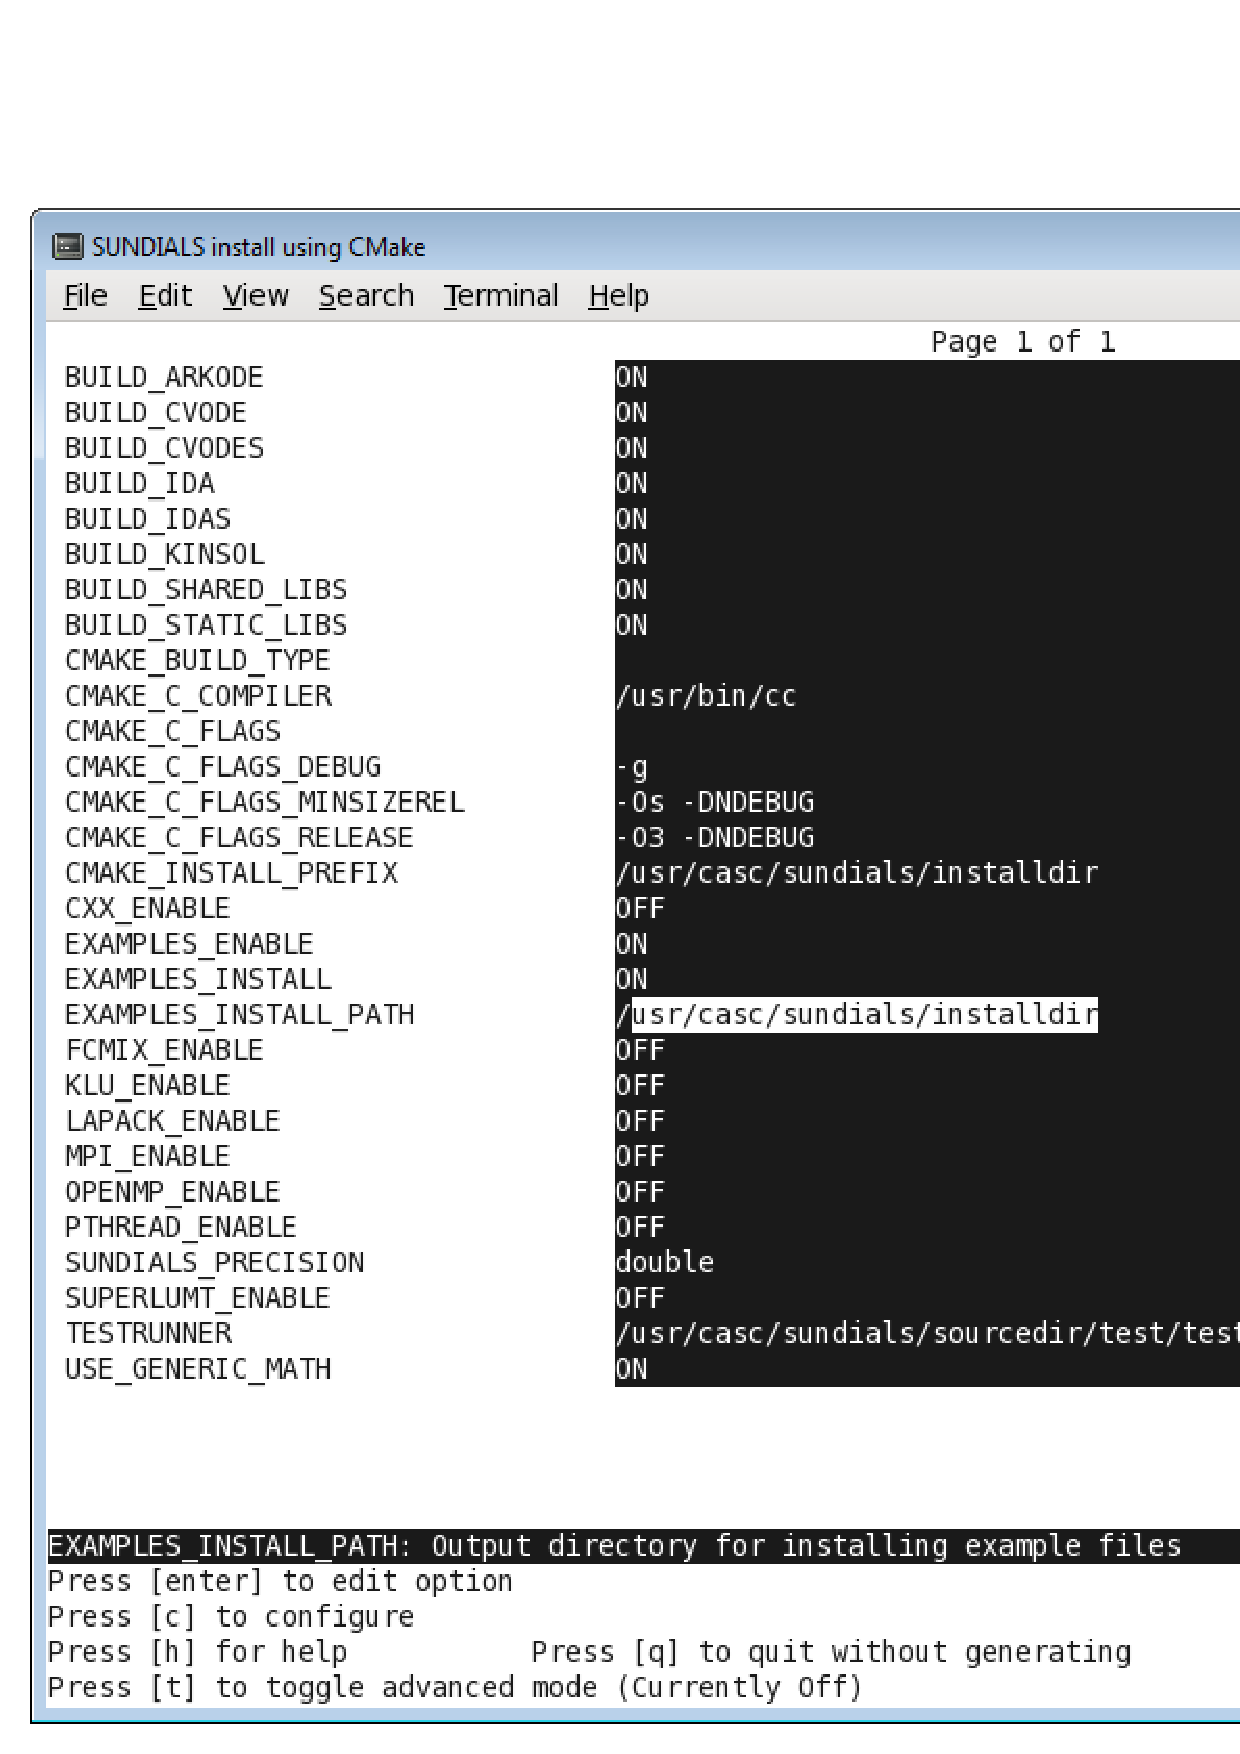
\includegraphics[width=\textwidth]{ccmakeprefix}}}
\caption [Changing the {\em instdir}]
{Changing the {\em instdir} for {\sundials} and
corresponding {\id examples} }
\label{f:ccmakeprefix}
\end{figure}

Pressing the (\id{g} key) will generate makefiles including all dependencies
and all rules to build {\sundials} on this system. 
Back at the command prompt, you can now run:

\begin{verbatim}
  % make
\end{verbatim}

To install {\sundials} in the installation directory specified in the configuration, simply run:

\begin{verbatim}
  % make install
\end{verbatim}

%%
%% *** NOTE: The TestRunner will not be distributed at this time.
%% *** Thus the following is commented out from the documentation.
%% TestRunner
%%
%\subsubsection*{Testing Installation}
%The distribution of {\sundials} includes several examples corresponding to the solvers to be
%installed. Also included in the source bundle is a test script: \id{testRunner}, configured by CMake
%to test the included examples.
%To run the tests, enter:

%\begin{verbatim}
%  % make test
%\end{verbatim}
%The output of \id{testRunner} should look similar to the screens in figure
%\ref{f:testrunner}. The success of each test is based on a line-by-line comparison of expected output files, bundled with the source code, with
%the output of the newly compiled examples. The file compare does allow some differences in rounding for float values.\\\\
%NOTE: Some tests may {\em fail} due to differences in machine architecture, compiler versions, third party libraries etc.{\warn}

%\begin{figure}[!ht]
%{\centerline{\includegraphics{figure=testrunnertop.eps,width=\textwidth}}}
%\vspace{3 mm}
%{\centerline{\includegraphics{figure=testrunnerbot.eps,width=\textwidth}}}
%\caption [Running {\em testRunner}]
%{Invoking {\em testRunner} with {\id make test} to execute all configured
%{\id examples} }
%\label{f:testrunner}
%\end{figure}

 
%%
%% Building from the command line
%%
\subsubsection*{Building from the command line}

Using CMake from the command line is simply a matter of specifying CMake variable settings
with the \id{cmake} command.  The following will build the default configuration:  

\begin{verbatim}
   % cmake -DCMAKE_INSTALL_PREFIX=/home/myname/sundials/instdir \
   > -DEXAMPLES_INSTALL_PATH=/home/myname/sundials/instdir/examples \
   > ../solverdir
   % make
   % make install
\end{verbatim}


\subsection{Configuration options (Unix/Linux)}\label{ss:configuration_options_nix}

A complete list of all available options for a CMake-based {\sundials}
configuration is provide below. Note that the default values shown are for 
a typical configuration on a Linux system and are provided as illustration only.

\begin{description}
\item[\id{BLAS\_ENABLE}] - 
  Enable BLAS support
  \\
  Default: OFF
  \\
  Note: Setting this option to ON will trigger additional CMake
  options. See additional information on building with BLAS enabled
  in \ref{ss:externallibs}.
\item[\id{BLAS\_LIBRARIES}] - 
  BLAS library
  \\
  Default: /usr/lib/libblas.so
  \\
  Note: CMake will search for libraries in your \id{LD\_LIBRARY\_PATH} prior
  to searching default system paths.
\item[\id{BUILD\_ARKODE}] - 
  Build the ARKODE library 
  \\
  Default: ON
\item[\id{BUILD\_CVODE}] - 
  Build the CVODE library 
  \\
  Default: ON
\item[\id{BUILD\_CVODES}] - 
  Build the CVODES library 
  \\
  Default: ON
\item[\id{BUILD\_IDA}] - 
   Build the IDA library 
  \\
   Default: ON
\item[\id{BUILD\_IDAS}] - 
  Build the IDAS library 
  \\
  Default: ON
\item[\id{BUILD\_KINSOL}] - 
  Build the KINSOL library 
  \\
  Default: ON
\item[\id{BUILD\_SHARED\_LIBS}] - 
  Build shared libraries
  \\
  Default: ON
\item[\id{BUILD\_STATIC\_LIBS}] - 
  Build static libraries
  \\
  Default: ON 
\item[\id{CMAKE\_BUILD\_TYPE}] -  
  Choose the type of build, options are: 
  \id{None} (CMAKE\_C\_FLAGS used), \id{Debug}, \id{Release},
  \id{RelWithDebInfo}, and \id{MinSizeRel}
  \\
  Default:
  \\
  Note: Specifying a build type will trigger the corresponding
  build type specific compiler flag options below which will be
  appended to the flags set by
  CMAKE\_{\textless}language{\textgreater}\_FLAGS. 
\item[\id{CMAKE\_C\_COMPILER}] - 
  C compiler
  \\
  Default: /usr/bin/cc 
\item[\id{CMAKE\_C\_FLAGS}] -  
  Flags for C compiler
  \\
  Default:
\item[\id{CMAKE\_C\_FLAGS\_DEBUG}] -      
  Flags used by the C compiler during debug builds
  \\
  Default: -g 
\item[\id{CMAKE\_C\_FLAGS\_MINSIZEREL}] -  
  Flags used by the C compiler during release minsize builds
  \\
  Default: -Os -DNDEBUG 
\item[\id{CMAKE\_C\_FLAGS\_RELEASE}] -    
  Flags used by the C compiler during release builds
  \\
  Default: -O3 -DNDEBUG 
\item[\id{CMAKE\_CXX\_COMPILER}] - 
  {\CPP} compiler
  \\
  Default: /usr/bin/c++
  \\
  Note: A {\CPP} compiler (and all related options) are only
  triggered if {\CPP} examples are enabled (\id{EXAMPLES\_ENABLE\_CXX}
  is ON). All {\sundials} solvers can be used from {\CPP} applications 
  by default without setting any additional configuration options.
\item[\id{CMAKE\_CXX\_FLAGS}] -
  Flags for {\CPP} compiler
  \\
  Default:
\item[\id{CMAKE\_CXX\_FLAGS\_DEBUG}] -
  Flags used by the {\CPP} compiler during debug builds
  \\
  Default: -g 
\item[\id{CMAKE\_CXX\_FLAGS\_MINSIZEREL}] -
  Flags used by the {\CPP} compiler during release minsize builds
  \\
  Default: -Os -DNDEBUG 
\item[\id{CMAKE\_CXX\_FLAGS\_RELEASE}] -
  Flags used by the {\CPP} compiler during release builds
  \\
  Default: -O3 -DNDEBUG
\item[\id{CMAKE\_Fortran\_COMPILER}] - 
  Fortran compiler
  \\
  Default: /usr/bin/gfortran
  \\
  Note: Fortran support (and all related options) are triggered only if
  either Fortran-C support is enabled (\id{FCMIX\_ENABLE} is ON) or
  BLAS/LAPACK support is enabled (\id{BLAS\_ENABLE} or \id{LAPACK\_ENABLE} is ON).
\item[\id{CMAKE\_Fortran\_FLAGS}] - 
  Flags for Fortran compiler
  \\
  Default:
\item[\id{CMAKE\_Fortran\_FLAGS\_DEBUG}] - 
  Flags used by the Fortran compiler during debug builds
  \\
  Default: -g
\item[\id{CMAKE\_Fortran\_FLAGS\_MINSIZEREL}] - 
  Flags used by the Fortran compiler during release minsize builds
  \\
  Default: -Os
\item[\id{CMAKE\_Fortran\_FLAGS\_RELEASE}] - 
  Flags used by the Fortran compiler during release builds
  \\
  Default: -O3
\item[\id{CMAKE\_INSTALL\_PREFIX}] -   
  Install path prefix, prepended onto install directories
  \\
  Default: /usr/local 
  \\
  Note: The user must have write access to the location specified through
  this option. Exported {\sundials} header files and libraries will be 
  installed under subdirectories \id{include} and \id{lib} of 
  \id{CMAKE\_INSTALL\_PREFIX}, respectively.
\item[\id{CUDA\_ENABLE}] -
  Build the {\sundials} {\cuda} vector module.
  \\
  Default: OFF
\item[\id{EXAMPLES\_ENABLE\_C}] -
  Build the {\sundials} {\CC} examples
  \\
  Default: ON
\item[\id{EXAMPLES\_ENABLE\_CUDA}] -
  Build the {\sundials} {\cuda} examples
  \\
  Default: OFF
  \\
  Note: You need to enable {\cuda} support to build these examples.
\item[\id{EXAMPLES\_ENABLE\_CXX}] -
  Build the {\sundials} {\CPP} examples
  \\
  Default: OFF
\item[\id{EXAMPLES\_ENABLE\_RAJA}] -
  Build the {\sundials} {\raja} examples
  \\
  Default: OFF
  \\
  Note: You need to enable {\cuda} and {\raja} support to build these examples.
\item[\id{EXAMPLES\_ENABLE\_F77}] -
  Build the {\sundials} Fortran77 examples
  \\
  Default: ON (if \id{FCMIX\_ENABLE} is ON)
\item[\id{EXAMPLES\_ENABLE\_F90}] -
  Build the {\sundials} Fortran90 examples
  \\
  Default: OFF
\item[\id{EXAMPLES\_INSTALL}] - 
  Install example files
  \\
  Default: ON
  \\
  Note: This option is triggered when any of the {\sundials}
  example programs are enabled \\
  (\id{EXAMPLES\_ENABLE\_$<$language$>$} is ON). If the user requires
  installation of example programs then the sources and sample output files
  for all {\sundials} modules that are currently enabled will be exported to
  the directory specified by \id{EXAMPLES\_INSTALL\_PATH}. A CMake configuration
  script will also be automatically generated and exported to the same directory.
  Additionally, if the configuration is done under a Unix-like system, makefiles
  for the compilation of the example programs (using the installed {\sundials} libraries)
  will be automatically generated and exported to the directory
  specified by \id{EXAMPLES\_INSTALL\_PATH}.
\item[\id{EXAMPLES\_INSTALL\_PATH}] - 
  Output directory for installing example files
  \\
  Default: /usr/local/examples
  \\
  Note: The actual default value for this option will be an \id{examples}
  subdirectory created under \id{CMAKE\_INSTALL\_PREFIX}.
\item[\id{FCMIX\_ENABLE}] - 
  Enable Fortran-C support   
  \\
  Default: OFF 
\item[\id{HYPRE\_ENABLE}] - 
  Enable \textit{hypre} support
  \\
  Default: OFF 
  \\
  Note: See additional information on building with \textit{hypre} enabled in
  \ref{ss:externallibs}. 
\item[\id{HYPRE\_INCLUDE\_DIR}] - 
  Path to \textit{hypre} header files
\item[\id{HYPRE\_LIBRARY\_DIR}] - 
  Path to \textit{hypre} installed library files
\item[\id{KLU\_ENABLE}] - 
  Enable KLU support
  \\
  Default: OFF 
  \\
  Note: See additional information on building with KLU enabled in
  \ref{ss:externallibs}. 
\item[\id{KLU\_INCLUDE\_DIR}] - 
  Path to SuiteSparse header files
\item[\id{KLU\_LIBRARY\_DIR}] - 
  Path to SuiteSparse installed library files
\item[\id{LAPACK\_ENABLE}] -  
  Enable LAPACK support
  \\
  Default: OFF
  \\
  Note: Setting this option to ON will trigger additional CMake
  options. See additional information on building with LAPACK enabled
  in \ref{ss:externallibs}.
\item[\id{LAPACK\_LIBRARIES}] - 
  LAPACK (and BLAS) libraries
  \\
  Default: /usr/lib/liblapack.so;/usr/lib/libblas.so
  \\
  Note: CMake will search for libraries in your \id{LD\_LIBRARY\_PATH} prior
  to searching default system paths.
\item[\id{MPI\_ENABLE}] -
  Enable MPI support (build the parallel nvector).
  \\
  Default: OFF 
  \\
  Note: Setting this option to ON will trigger several additional options
  related to MPI.
\item[\id{MPI\_C\_COMPILER}] -
  \id{mpicc} program
  \\
  Default: 
\item[\id{MPI\_CXX\_COMPILER}] -
  \id{mpicxx} program
  \\
  Default: 
  \\
  Note: This option is triggered only if MPI is enabled
  (\id{MPI\_ENABLE} is ON) and {\CPP} examples are enabled
  (\id{EXAMPLES\_ENABLE\_CXX} is ON). All {\sundials}
  solvers can be used from {\CPP} MPI applications by default
  without setting any additional configuration options other than
  \id{MPI\_ENABLE}.
\item[\id{MPI\_Fortran\_COMPILER}] -
  \id{mpif77} or \id{mpif90} program
  \\
  Default: 
  \\
  Note: This option is triggered only if MPI is enabled
  (\id{MPI\_ENABLE} is ON), Fortran-C support is enabled
  (\id{FCMIX\_ENABLE} is ON), and Fortran77 or Fortran90
  examples are enabled (\id{EXAMPLES\_ENABLE\_F77} or
  \id{EXAMPLES\_ENABLE\_F90} are ON).
\item[\id{MPIEXEC}] -
  Specify the executable for running MPI programs
  \\
  Default: \id{mpirun}
  \\
  Note: This option is triggered only if MPI is enabled
  (\id{MPI\_ENABLE} is ON).
  %% \\
  %% Note: This can either be set to \id{mpirun} for OpenMPI or \id{srun} if jobs are
  %% managed by \id{SLURM} - Simple Linux Utility for Resource Management as exists on
  %% LLNL's high performance computing clusters. 
\item[\id{OPENMP\_ENABLE}] -
  Enable OpenMP support (build the OpenMP nvector).
  \\
  Default: OFF 
\item[\id{PETSC\_ENABLE}] - 
  Enable PETSc support
  \\
  Default: OFF 
  \\
  Note: See additional information on building with PETSc enabled
  in \ref{ss:externallibs}.
\item[\id{PETSC\_INCLUDE\_DIR}] -
  Path to PETSc header files
\item[\id{PETSC\_LIBRARY\_DIR}] - 
  Path to PETSc installed library files
\item[\id{PTHREAD\_ENABLE}] -  
  Enable Pthreads support (build the Pthreads nvector).
  \\
  Default: OFF 
\item[\id{RAJA\_ENABLE}] - 
  Enable {\raja} support (build the {\raja} nvector).
  \\
  Default: OFF 
  \\
  Note: You need to enable {\cuda} in order to build the {\raja} vector module.
\item[\id{SUNDIALS\_F77\_FUNC\_CASE}] - \textbf{advanced option} -
  Specify the case to use in the Fortran name-mangling scheme, options
  are: \id{lower} or \id{upper}
  \\
  Default:
  \\
  Note: The build system will attempt to infer the Fortran
  name-mangling scheme using the Fortran compiler. This option should
  only be used if a Fortran compiler is not available or to override
  the inferred or default (\id{lower}) scheme if one can not be
  determined. If used, \id{SUNDIALS\_F77\_FUNC\_UNDERSCORES} must also
  be set.
\item[\id{SUNDIALS\_F77\_FUNC\_UNDERSCORES}] - \textbf{advanced option} -
  Specify the number of underscores to append in the Fortran
  name-mangling scheme, options are: \id{none}, \id{one}, or \id{two}
  \\
  Default:
  \\
  Note: The build system will attempt to infer the Fortran
  name-mangling scheme using the Fortran compiler. This option should
  only be used if a Fortran compiler is not available or to override
  the inferred or default (\id{one}) scheme if one can not be
  determined. If used, \id{SUNDIALS\_F77\_FUNC\_CASE} must also be set.
\item[\id{SUNDIALS\_INDEX\_TYPE}] - 
  Integer type used for {\sundials} indices, options are: \id{int32\_t} or \id{int64\_t}
  \\
  Default: \id{int64\_t}
\item[\id{SUNDIALS\_PRECISION}] -   
  Precision used in {\sundials}, options are: \id{double}, \id{single}, or \id{extended}
  \\
  Default: \id{double}
\item[\id{SUPERLUMT\_ENABLE}] - 
  Enable SuperLU\_MT support   
  \\
  Default: OFF 
  \\
  Note: See additional information on building with SuperLU\_MT enabled
  in \ref{ss:externallibs}.
\item[\id{SUPERLUMT\_INCLUDE\_DIR}] - 
  Path to SuperLU\_MT header files (typically SRC directory)
\item[\id{SUPERLUMT\_LIBRARY\_DIR}] - 
  Path to SuperLU\_MT installed library files
\item[\id{SUPERLUMT\_THREAD\_TYPE}] - 
  Must be set to Pthread or OpenMP
  \\
  Default: Pthread
\item[\id{USE\_GENERIC\_MATH}] -   
  Use generic (stdc) math libraries
  \\
  Default: ON 
\end{description}

\subsubsection*{xSDK Configuration Options}

{\sundials} supports CMake configuration options defined by the
Extreme-scale Scientific Software Development Kit (xSDK) community
policies (see {\tt https://xsdk.info} for more information). xSDK
CMake options are unused by default but may be activated by setting
\id{USE\_XSDK\_DEFAULTS} to ON.

{\warn} When xSDK options are active, they will overwrite the
corresponding {\sundials} option and may have different default values
(see details below). As such the equivalent {\sundials} options should
not be used when configuring with xSDK options. In the GUI front end
to CMake (\id{ccmake}), setting \id{USE\_XSDK\_DEFAULTS} to ON will
hide the corresponding {\sundials} options as advanced CMake variables.
During configuration, messages are output detailing
which xSDK flags are active and the equivalent {\sundials} options
that are replaced. Below is a complete list xSDK options and the
corresponding {\sundials} options if applicable.

\begin{description}
\item[\id{TPL\_BLAS\_LIBRARIES}] - 
  BLAS library
  \\
  Default: /usr/lib/libblas.so
  \\
  {\sundials} equivalent: \id{BLAS\_LIBRARIES}
  \\
  Note: CMake will search for libraries in your \id{LD\_LIBRARY\_PATH} prior
  to searching default system paths.
\item[\id{TPL\_ENABLE\_BLAS}] - 
  Enable BLAS support
  \\
  Default: OFF
  \\
  {\sundials} equivalent: \id{BLAS\_ENABLE}
\item[\id{TPL\_ENABLE\_HYPRE}] - 
  Enable \textit{hypre} support
  \\
  Default: OFF
  \\
  {\sundials} equivalent: \id{HYPRE\_ENABLE}
\item[\id{TPL\_ENABLE\_KLU}] - 
  Enable KLU support
  \\
  Default: OFF
  \\
  {\sundials} equivalent: \id{KLU\_ENABLE}
\item[\id{TPL\_ENABLE\_PETSC}] - 
  Enable PETSc support
  \\
  Default: OFF
  \\
  {\sundials} equivalent: \id{PETSC\_ENABLE}
\item[\id{TPL\_ENABLE\_LAPACK}] - 
  Enable LAPACK support
  \\
  Default: OFF
  \\
  {\sundials} equivalent: \id{LAPACK\_ENABLE}
\item[\id{TPL\_ENABLE\_SUPERLUMT}] - 
  Enable SuperLU\_MT support
  \\
  Default: OFF
  \\
  {\sundials} equivalent: \id{SUPERLUMT\_ENABLE}
\item[\id{TPL\_HYPRE\_INCLUDE\_DIRS}] - 
  Path to \textit{hypre} header files
  \\
  {\sundials} equivalent: \id{HYPRE\_INCLUDE\_DIR}
\item[\id{TPL\_HYPRE\_LIBRARIES}] - 
  \textit{hypre} library
  \\
  {\sundials} equivalent: N/A
\item[\id{TPL\_KLU\_INCLUDE\_DIRS}] - 
  Path to KLU header files
  \\
  {\sundials} equivalent: \id{KLU\_INCLUDE\_DIR}
\item[\id{TPL\_KLU\_LIBRARIES}] - 
  KLU library
  \\
  {\sundials} equivalent: N/A
\item[\id{TPL\_LAPACK\_LIBRARIES}] - 
  LAPACK (and BLAS) libraries
  \\
  Default: /usr/lib/liblapack.so;/usr/lib/libblas.so
  \\
  {\sundials} equivalent: \id{LAPACK\_LIBRARIES}
  \\
  Note: CMake will search for libraries in your \id{LD\_LIBRARY\_PATH} prior
  to searching default system paths.
\item[\id{TPL\_PETSC\_INCLUDE\_DIRS}] - 
  Path to PETSc header files
  \\
  {\sundials} equivalent: \id{PETSC\_INCLUDE\_DIR}
\item[\id{TPL\_PETSC\_LIBRARIES}] - 
  PETSc library
  \\
  {\sundials} equivalent: N/A
\item[\id{TPL\_SUPERLUMT\_INCLUDE\_DIRS}] - 
  Path to SuperLU\_MT header files
  \\
  {\sundials} equivalent: \id{SUPERLUMT\_INCLUDE\_DIR}
\item[\id{TPL\_SUPERLUMT\_LIBRARIES}] - 
  SuperLU\_MT library
  \\
  {\sundials} equivalent: N/A
\item[\id{TPL\_SUPERLUMT\_THREAD\_TYPE}] - 
  SuperLU\_MT library thread type
  \\
  {\sundials} equivalent: \id{SUPERLUMT\_THREAD\_TYPE}
\item[\id{USE\_XSDK\_DEFAULTS}] - 
  Enable xSDK default configuration settings
  \\
  Default: OFF
  \\
  {\sundials} equivalent: N/A
  \\
  Note: Enabling xSDK defaults also sets \id{CMAKE\_BUILD\_TYPE} to \id{Debug}
\item[\id{XSDK\_ENABLE\_FORTRAN}] -
  Enable {\sundials} Fortran interface
  \\
  Default: OFF
  \\
  {\sundials} equivalent: \id{FCMIX\_ENABLE}
\item[\id{XSDK\_INDEX\_SIZE}] -
  Integer size (bits) used for indices in {\sundials}, options are: \id{32} or \id{64}
  \\
  Default: \id{32}
  \\
  {\sundials} equivalent: \id{SUNDIALS\_INDEX\_TYPE}
\item[\id{XSDK\_PRECISION}] -
  Precision used in {\sundials}, options are: \id{double}, \id{single}, or \id{quad}
  \\
  Default: \id{double}
  \\
  {\sundials} equivalent: \id{SUNDIALS\_PRECISION}
\end{description}



%%===============================================================================

\subsection{Configuration examples}

The following examples will help demonstrate usage of the CMake configure options.

\noindent To configure {\sundials} using the default C and Fortran compilers,
and default \id{mpicc} and \id{mpif77} parallel compilers, 
enable compilation of examples, and install libraries, headers, and
example sources under subdirectories of
\id{/home/myname/sundials/}, use:

\begin{verbatim}
   % cmake \
   > -DCMAKE_INSTALL_PREFIX=/home/myname/sundials/instdir \
   > -DEXAMPLES_INSTALL_PATH=/home/myname/sundials/instdir/examples \
   > -DMPI_ENABLE=ON \
   > -DFCMIX_ENABLE=ON \
   > /home/myname/sundials/solverdir
   %
   % make install
   % 
\end{verbatim}

\noindent To disable installation of the examples, use:
\begin{verbatim}
   % cmake \
   > -DCMAKE_INSTALL_PREFIX=/home/myname/sundials/instdir \
   > -DEXAMPLES_INSTALL_PATH=/home/myname/sundials/instdir/examples \
   > -DMPI_ENABLE=ON \
   > -DFCMIX_ENABLE=ON \
   > -DEXAMPLES_INSTALL=OFF \
   > /home/myname/sundials/solverdir
   %
   % make install
   % 
\end{verbatim}

%%===============================================================================
\subsection{Working with external Libraries} \label{ss:externallibs}

The {\sundials} suite contains many options to enable implementation flexibility
when developing solutions. The following are some notes addressing specific configurations
when using the supported third party libraries.
When building {\sundials} as a shared library external libraries any
used with {\sundials} must also be build as a shared library or as a
static library compiled with the \id{-fPIC} flag.{\warn}

\subsubsection*{Building with BLAS}
{\sundials} does not utilize BLAS directly but it may be needed by other
external libraries that {\sundials} can be built with (e.g. LAPACK,
PETSc, SuperLU\_MT, etc.). To enable BLAS, set the \id{BLAS\_ENABLE}
option to \id{ON}. If the directory containing the BLAS library is in
the \id{LD\_LIBRARY\_PATH} environment variable, CMake will set the
\id{BLAS\_LIBRARIES} variable accordingly, otherwise CMake will
attempt to find the BLAS library in standard system locations. To
explicitly tell CMake what libraries to use, the \id{BLAS\_LIBRARIES}
variable can be set to the desired library. Example:
\begin{verbatim}
   % cmake \
   > -DCMAKE_INSTALL_PREFIX=/home/myname/sundials/instdir \
   > -DEXAMPLES_INSTALL_PATH=/home/myname/sundials/instdir/examples \
   > -DBLAS_ENABLE=ON \
   > -DBLAS_LIBRARIES=/myblaspath/lib/libblas.so \
   > -DSUPERLUMT_ENABLE=ON \
   > -DSUPERLUMT_INCLUDE_DIR=/mysuperlumtpath/SRC
   > -DSUPERLUMT_LIBRARY_DIR=/mysuperlumtpath/lib
   > /home/myname/sundials/solverdir
   %
   % make install
   % 
\end{verbatim}
{\warn}When allowing CMake to automatically locate the LAPACK library,
CMake \textit{may} also locate the corresponding BLAS library.

If a working Fortran compiler is not available to infer the Fortran
name-mangling scheme, the options \id{SUNDIALS\_F77\_FUNC\_CASE} and
\id{SUNDIALS\_F77\_FUNC\_UNDERSCORES} \textit{must} be set in order to
bypass the check for a Fortran compiler and define the name-mangling
scheme. The defaults for these options in earlier versions of
{\sundials} were \id{lower} and \id{one} respectively.


\subsubsection*{Building with LAPACK}
To enable LAPACK, set the \id{LAPACK\_ENABLE} option to \id{ON}.
If the directory containing the LAPACK library is in the
\id{LD\_LIBRARY\_PATH} environment variable, CMake will set the
\id{LAPACK\_LIBRARIES} variable accordingly, otherwise CMake will
attempt to find the LAPACK library in standard system locations. To
explicitly tell CMake what library to use, the \id{LAPACK\_LIBRARIES}
variable can be set to the desired libraries. {\warn}When setting
the LAPACK location explicitly the location of the corresponding BLAS
library will also need to be set. Example:
\begin{verbatim}
   % cmake \
   > -DCMAKE_INSTALL_PREFIX=/home/myname/sundials/instdir \
   > -DEXAMPLES_INSTALL_PATH=/home/myname/sundials/instdir/examples \
   > -DBLAS_ENABLE=ON \
   > -DBLAS_LIBRARIES=/mylapackpath/lib/libblas.so \
   > -DLAPACK_ENABLE=ON \
   > -DLAPACK_LIBRARIES=/mylapackpath/lib/liblapack.so \
   > /home/myname/sundials/solverdir
   %
   % make install
   % 
\end{verbatim}
{\warn}When allowing CMake to automatically locate the LAPACK library,
CMake \textit{may} also locate the corresponding BLAS library.

If a working Fortran compiler is not available to infer the Fortran
name-mangling scheme, the options \id{SUNDIALS\_F77\_FUNC\_CASE} and
\id{SUNDIALS\_F77\_FUNC\_UNDERSCORES} \textit{must} be set in order to
bypass the check for a Fortran compiler and define the name-mangling
scheme. The defaults for these options in earlier versions of
{\sundials} were \id{lower} and \id{one} respectively.

\subsubsection*{Building with KLU}
The KLU libraries are part of SuiteSparse, a suite of sparse matrix software,
available from the Texas A\&M University website: {\tt http://faculty.cse.tamu.edu/davis/suitesparse.html}.
{\sundials} has been tested with SuiteSparse version 4.5.3.
To enable KLU, set \id{KLU\_ENABLE} to \id{ON}, set \id{KLU\_INCLUDE\_DIR} to the \id{include}
path of the KLU installation and set \id{KLU\_LIBRARY\_DIR} to the \id{lib} path of the KLU installation.
The CMake configure will result in populating the following variables: \id{AMD\_LIBRARY},
\id{AMD\_LIBRARY\_DIR}, \id{BTF\_LIBRARY}, \id{BTF\_LIBRARY\_DIR},
\id{COLAMD\_LIBRARY}, \id{COLAMD\_LIBRARY\_DIR}, and
\newline\id{KLU\_LIBRARY}.

\subsubsection*{Building with SuperLU\_MT}
The SuperLU\_MT libraries are available for download from the Lawrence Berkeley National Laboratory website:
{\tt http://crd-legacy.lbl.gov/$\sim$xiaoye/SuperLU/\#superlu\_mt}. 
{\sundials} has been tested with SuperLU\_MT version 3.1. 
To enable SuperLU\_MT, set  \id{SUPERLUMT\_ENABLE} to \id{ON}, set \id{SUPERLUMT\_INCLUDE\_DIR}
to the \id{SRC} path of the SuperLU\_MT installation, and set the variable
\newline\id{SUPERLUMT\_LIBRARY\_DIR} to the \id{lib} path of the SuperLU\_MT installation.
At the same time, the variable
\id{SUPERLUMT\_THREAD\_TYPE} must be set to either \id{Pthread} or \id{OpenMP}.

\noindent Do not mix thread types when building {\sundials} solvers.
If threading is enabled for {\sundials} by having either \id{OPENMP\_ENABLE} or \id{PTHREAD\_ENABLE} set to \id{ON}
then SuperLU\_MT should be set to use the same threading type.{\warn}

\subsubsection*{Building with PETSc}
The PETSc libraries are available for download from the Argonne National Laboratory website:
{\tt http://www.mcs.anl.gov/petsc}. 
{\sundials} has been tested with PETSc version 3.7.2. 
To enable PETSc, set  \id{PETSC\_ENABLE} to \id{ON}, set \id{PETSC\_INCLUDE\_DIR}
to the \id{include} path of the PETSc installation, and set the variable
\id{PETSC\_LIBRARY\_DIR} to the \id{lib} path of the PETSc installation.


\subsubsection*{Building with \textit{hypre}}
The \textit{hypre} libraries are available for download from the Lawrence Livermore
National Laboratory website: {\tt http://computation.llnl.gov/projects/hypre}.
%{\tt http://computation.llnl.gov/projects/hypre-scalable-linear-solvers-multigrid-methods}.
{\sundials} has been tested with \textit{hypre} version 2.11.1. 
To enable \textit{hypre}, set  \id{HYPRE\_ENABLE} to \id{ON}, set \id{HYPRE\_INCLUDE\_DIR}
to the \id{include} path of the \textit{hypre} installation, and set the variable
\id{HYPRE\_LIBRARY\_DIR} to the \id{lib} path of the \textit{hypre} installation.

\subsubsection*{Building with CUDA}
{\sundials} {\cuda} modules and examples have been tested with version 8.0 of the 
{\cuda} toolkit. To build them, you need to install the Toolkit and compatible
NVIDIA drivers. Both are available for download from the NVIDIA website:
{\tt https://developer.nvidia.com/cuda-downloads}. To enable {\cuda}, 
set \id{CUDA\_ENABLE} to \id{ON}. If {\cuda} is installed in a
nonstandard location, you may be prompted to set the variable
\id{CUDA\_TOOLKIT\_ROOT\_DIR} with your {\cuda} Toolkit installation
path. To enable {\cuda} examples, set \id{EXAMPLES\_ENABLE\_CUDA} to \id{ON}.

\subsubsection*{Building with RAJA}
{\raja} is a performance portability layer developed by Lawrence
Livermore National Laboratory and can be obtained from {\tt https://github.com/LLNL/RAJA}.
{\sundials} {\raja} modules and examples have been tested with {\raja}
version 0.3. Building {\sundials} {\raja} modules requires a
{\cuda}-enabled {\raja} installation. To enable {\raja}, set
\id{CUDA\_ENABLE} and \id{RAJA\_ENABLE} to \id{ON}. If {\raja} is
installed in a nonstandard location you will be prompted to set the
variable \id{RAJA\_DIR} with the path to the {\raja} CMake
configuration file. To enable building the {\raja} examples set
\id{EXAMPLES\_ENABLE\_RAJA} to \id{ON}.

\subsection{Testing the build and installation}

If {\sundials} was configured with
\id{EXAMPLES\_ENABLE\_$<$language$>$} options to \id{ON}, then a set of
regression tests can be run after building with the \id{make} command
by running: 
\begin{verbatim}
  % make test
\end{verbatim}
Additionally, if \id{EXAMPLES\_INSTALL} was also set to \id{ON}, then
a set of smoke tests can be run after installing with the \id{make install} 
command by running:
\begin{verbatim}
  % make test_install
\end{verbatim}

%%===============================================================================
\section{Building and Running Examples}
%%===============================================================================
Each of the {\sundials} solvers is distributed with a set of examples
demonstrating basic usage. To build and install the examples, set at
least of the \id{EXAMPLES\_ENABLE\_$<$language$>$} options to \id{ON}, and
set \id{EXAMPLES\_INSTALL} to \id{ON}.
Specify the installation path for the examples with the variable \id{EXAMPLES\_INSTALL\_PATH}. CMake will generate
\id{CMakeLists.txt} configuration files (and \id{Makefile} files if on Linux/Unix) that reference the
{\em installed} {\sundials} headers and libraries.

Either the \id{CMakeLists.txt} file or the traditional \id{Makefile} may be used to build the examples
as well as serve as a template for creating user developed solutions.
To use the supplied \id{Makefile} simply run \id{make} to compile and generate the executables.
To use CMake from within the installed example directory, run \id{cmake} (or \id{ccmake} to use the GUI)
followed by \id{make} to compile the example code.
Note that if CMake is used, it will overwrite the traditional \id{Makefile} with a new CMake-generated \id{Makefile}.
The resulting output from running the examples can be compared with example output bundled
in the {\sundials} distribution.

\noindent NOTE: There will potentially be differences in the output due to machine architecture, compiler versions,
use of third party libraries etc.{\warn} 


%%===============================================================================
\section{Configuring, building, and installing  on Windows}\label{s:cmake_windows}
%%===============================================================================
CMake can also be used to build {\sundials} on Windows. To build {\sundials} for
use with Visual Studio the following steps should be performed:
\begin{enumerate}
\item Unzip the downloaded tar file(s) into a directory. This will be the {\em solverdir} 
\item Create a separate {\em builddir}
\item Open a Visual Studio Command Prompt and cd to {\em builddir}
\item Run cmake-gui ../{\em solverdir}
\begin{enumerate}
\item Hit Configure
\item Check/Uncheck solvers to be built
\item Change CMAKE\_INSTALL\_PREFIX to {\em instdir}
\item Set other options as desired
\item Hit Generate
\end{enumerate}
\item Back in the VS Command Window:
\begin{enumerate}
\item Run msbuild ALL\_BUILD.vcxproj
\item Run msbuild INSTALL.vcxproj
\end{enumerate} 
\end{enumerate}

\noindent The resulting libraries will be in the {\em instdir}.
\noindent The {\sundials} project can also now be opened in Visual Studio.
Double click on the ALL\_BUILD.vcxproj file to open the project.
Build the whole {\em solution} to create the {\sundials} libraries.
To use the {\sundials} libraries in your own projects, you must
set the include directories for your project,
add the {\sundials} libraries to your project solution,
and set the {\sundials} libraries as dependencies for your project.

%%===============================================================================
\section{Installed libraries and exported header files}
%%===============================================================================

Using the CMake {\sundials} build system, the command
\begin{verbatim}
   % make install
\end{verbatim}
will install the libraries under {\em libdir} and the public header
files under {\em includedir}. The values for these directories are
{\em instdir}\id{/lib} and {\em instdir}\id{/include},
respectively. The location can be changed by setting the CMake variable \id{CMAKE\_INSTALL\_PREFIX}.
Although all installed libraries reside under {\em libdir}\id{/lib}, the public header files
are further organized into subdirectories under {\em includedir}\id{/include}.

The installed libraries and exported header files are listed for
reference in Table \ref{t:sundials_files}.
The file extension .{\em lib}
is typically \id{.so} for shared libraries and \id{.a} for static libraries.
Note that, in the Tables, names are relative to {\em libdir}
for libraries and to {\em includedir} for header files.

A typical user program need not explicitly include any of the shared
{\sundials} header files from under the {\em includedir}\id{/include}\id{/sundials}
directory since they are explicitly included by the appropriate solver
header files ({\em e.g.}, \id{cvode\_dense.h} includes
\id{sundials\_dense.h}). However, it is both legal and safe to do so,
and would be useful, for example, if the functions declared in \id{sundials\_dense.h} 
are to be used in building a preconditioner.

%---------------------------------------------------------------------------
% Table of installed files
%---------------------------------------------------------------------------

\newlength{\colLenOne}
\settowidth{\colLenOne}{{\sunlinsollapdense}}

\newlength{\colLenTwo}
\settowidth{\colLenTwo}{Header files}

\newlength{\colLenThree}
\setlength{\colLenThree}{\textwidth}
\addtolength{\colLenThree}{-0.5in}
\addtolength{\colLenThree}{-\colLenOne}
\addtolength{\colLenThree}{-\colLenTwo}

%\caption{{\sundials} libraries and header files (cont.)}\label{t:sundials_files2}

\tablecaption{{\sundials} libraries and header files}\label{t:sundials_files}
\tablefirsthead{\hline}
\tablehead{\hline \multicolumn{4}{|l|}{\small\slshape continued from last page} \\
           \hline}
\tabletail{\hline \multicolumn{4}{|r|}{\small\slshape continued on next page} \\ \hline}
\begin{xtabular}{|p{\colLenOne}|p{\colLenTwo}|p{0.5\colLenThree} p{0.5\colLenThree}|}

%% --------------------------------------------------
{\shared}
 & Libraries    & n/a  & \\
\cline{2-4}
 & Header files & sundials/sundials\_config.h        & sundials/sundials\_fconfig.h  \\
 &              & sundials/sundials\_types.h         & sundials/sundials\_math.h     \\
 &              & sundials/sundials\_nvector.h       & sundials/sundials\_fnvector.h \\
 &              & sundials/sundials\_iterative.h     & sundials/sundials\_direct.h   \\
 &              & sundials/sundials\_dense.h         & sundials/sundials\_band.h     \\
 &              & sundials/sundials\_matrix.h        & sundials/sundials\_version.h  \\
 &              & sundials/sundials\_linearsolver.h  & \\
\hline
%% --------------------------------------------------
{\nvecs}
 & Libraries    & libsundials\_nvecserial.{\em lib} & libsundials\_fnvecserial.a \\ 
\cline{2-4}
 & Header files & nvector/nvector\_serial.h         & \\ 
\hline
%% --------------------------------------------------
{\nvecp}
 & Libraries    & libsundials\_nvecparallel.{\em lib} & libsundials\_fnvecparallel.a \\
\cline{2-4}
 & Header files & nvector/nvector\_parallel.h         & \\
\hline
%% --------------------------------------------------
{\nvecopenmp}
 & Libraries    & libsundials\_nvecopenmp.{\em lib} & libsundials\_fnvecopenmp.a \\ 
\cline{2-4}
 & Header files & nvector/nvector\_openmp.h         & \\ 
\hline
%% --------------------------------------------------
{\nvecpthreads}
 & Libraries    & libsundials\_nvecpthreads.{\em lib} & libsundials\_fnvecpthreads.a \\ 
\cline{2-4}
 & Header files & nvector/nvector\_pthreads.h         & \\ 
\hline
%% --------------------------------------------------
{\nvecph}
 & Libraries    & libsundials\_nvecparhyp.{\em lib} & \\
\cline{2-4}
 & Header files & nvector/nvector\_parhyp.h         & \\ 
\hline
%% --------------------------------------------------
{\nvecpetsc}
 & Libraries    & libsundials\_nvecpetsc.{\em lib} & \\ 
\cline{2-4}
 & Header files & nvector/nvector\_petsc.h         & \\ 
\hline
%% --------------------------------------------------
{\nveccuda}
 & Libraries    & libsundials\_nveccuda.{\em lib}     & \\ 
\cline{2-4}
 & Header files & nvector/nvector\_cuda.h             & \\
 &              & nvector/cuda/ThreadPartitioning.hpp & \\
 &              & nvector/cuda/Vector.hpp             & \\
 &              & nvector/cuda/VectorKernels.cuh      & \\
\hline
%% --------------------------------------------------
{\nvecraja}
 & Libraries    & libsundials\_nvecraja.{\em lib} & \\ 
\cline{2-4}
 & Header files & nvector/nvector\_raja.h         & \\
 &              & nvector/raja/Vector.hpp         & \\
\hline
%% --------------------------------------------------
{\sunmatband}
 & Libraries    & libsundials\_sunmatrixband.{\em lib} & \\ 
 &              & libsundials\_fsunmatrixband.a        & \\ 
\cline{2-4}
 & Header files & sunmatrix/sunmatrix\_band.h          & \\ 
\hline
%% --------------------------------------------------
{\sunmatdense}
 & Libraries    & libsundials\_sunmatrixdense.{\em lib} & \\
 &              & libsundials\_fsunmatrixdense.a        & \\
\cline{2-4}
 & Header files & sunmatrix/sunmatrix\_dense.h          & \\
\hline
%% --------------------------------------------------
{\sunmatsparse}
 & Libraries    & libsundials\_sunmatrixsparse.{\em lib} & \\ 
 &              & libsundials\_fsunmatrixsparse.a        & \\ 
\cline{2-4}
 & Header files & sunmatrix/sunmatrix\_sparse.h          & \\ 
\hline
%% --------------------------------------------------
{\sunlinsolband}
 & Libraries    & libsundials\_sunlinsolband.{\em lib} & \\ 
 &              & libsundials\_fsunlinsolband.a        & \\ 
\cline{2-4}
 & Header files & sunlinsol/sunlinsol\_band.h          & \\ 
\hline
%% --------------------------------------------------
{\sunlinsoldense}
 & Libraries    & libsundials\_sunlinsoldense.{\em lib} & \\ 
 &              & libsundials\_fsunlinsoldense.a        & \\ 
\cline{2-4}
 & Header files & sunlinsol/sunlinsol\_dense.h          & \\ 
\hline
%% --------------------------------------------------
{\sunlinsolklu}
 & Libraries    & libsundials\_sunlinsolklu.{\em lib} & \\ 
 &              & libsundials\_fsunlinsolklu.a        & \\ 
\cline{2-4}
 & Header files & sunlinsol/sunlinsol\_klu.h          & \\ 
\hline
%% --------------------------------------------------
{\sunlinsollapband}
 & Libraries    & libsundials\_sunlinsollapackband.{\em lib} & \\ 
 &              & libsundials\_fsunlinsollapackband.a        & \\ 
\cline{2-4}
 & Header files & sunlinsol/sunlinsol\_lapackband.h          & \\ 
\hline
%% --------------------------------------------------
{\sunlinsollapdense}
 & Libraries    & libsundials\_sunlinsollapackdense.{\em lib} & \\ 
 &              & libsundials\_fsunlinsollapackdense.a        & \\ 
\cline{2-4}
 & Header files & sunlinsol/sunlinsol\_lapackdense.h          & \\ 
\hline
%% --------------------------------------------------
{\sunlinsolpcg}
 & Libraries    & libsundials\_sunlinsolpcg.{\em lib} & \\ 
 &              & libsundials\_fsunlinsolpcg.a        & \\ 
\cline{2-4}
 & Header files & sunlinsol/sunlinsol\_pcg.h          & \\ 
\hline
%% --------------------------------------------------
{\sunlinsolspbcgs}
 & Libraries    & libsundials\_sunlinsolspbcgs.{\em lib} & \\ 
 &              & libsundials\_fsunlinsolspbcgs.a        & \\ 
\cline{2-4}
 & Header files & sunlinsol/sunlinsol\_spbcgs.h          & \\ 
\hline
%% --------------------------------------------------
{\sunlinsolspfgmr}
 & Libraries    & libsundials\_sunlinsolspfgmr.{\em lib} & \\ 
 &              & libsundials\_fsunlinsolspfgmr.a        & \\ 
\cline{2-4}
 & Header files & sunlinsol/sunlinsol\_spfgmr.h          & \\ 
\hline
%% --------------------------------------------------
{\sunlinsolspgmr}
 & Libraries    & libsundials\_sunlinsolspgmr.{\em lib} & \\ 
 &              & libsundials\_fsunlinsolspgmr.a        & \\ 
\cline{2-4}
 & Header files & sunlinsol/sunlinsol\_spgmr.h          & \\ 
\hline
%% --------------------------------------------------
{\sunlinsolsptfqmr}
 & Libraries    & libsundials\_sunlinsolsptfqmr.{\em lib} & \\ 
 &              & libsundials\_fsunlinsolsptfqmr.a        & \\ 
\cline{2-4}
 & Header files & sunlinsol/sunlinsol\_sptfqmr.h          & \\ 
\hline
%% --------------------------------------------------
{\sunlinsolslumt}
 & Libraries    & libsundials\_sunlinsolsuperlumt.{\em lib} & \\ 
 &              & libsundials\_fsunlinsolsuperlumt.a        & \\ 
\cline{2-4}
 & Header files & sunlinsol/sunlinsol\_superlumt.h          & \\ 
\hline
%% --------------------------------------------------
{\cvode}
 & Libraries    & libsundials\_cvode.{\em lib} & libsundials\_fcvode.a \\
\cline{2-4}
 & Header files & cvode/cvode.h                & cvode/cvode\_impl.h   \\
 &              & cvode/cvode\_direct.h        & cvode/cvode\_spils.h  \\
 &              & cvode/cvode\_bandpre.h       & cvode/cvode\_bbdpre.h \\
\hline
%% --------------------------------------------------
{\cvodes}
 & Libraries    & libsundials\_cvodes.{\em lib} & \\
\cline{2-4}
 & Header files & cvodes/cvodes.h               & cvodes/cvodes\_impl.h   \\
 &              & cvodes/cvodes\_direct.h       & cvodes/cvodes\_spils.h  \\
 &              & cvodes/cvodes\_bandpre.h      & cvodes/cvodes\_bbdpre.h \\
\hline
%% --------------------------------------------------
{\arkode}
 & Libraries    & libsundials\_arkode.{\em lib} & libsundials\_farkode.a \\
\cline{2-4}
 & Header files & arkode/arkode.h               & arkode/arkode\_impl.h   \\
 &              & arkode/arkode\_direct.h       & arkode/arkode\_spils.h  \\
 &              & arkode/arkode\_bandpre.h      & arkode/arkode\_bbdpre.h \\
\hline
%% --------------------------------------------------
{\ida}
 & Libraries    & libsundials\_ida.{\em lib} & libsundials\_fida.a \\
\cline{2-4}
 & Header files & ida/ida.h                  & ida/ida\_impl.h     \\
 &              & ida/ida\_direct.h          & ida/ida\_spils.h    \\
 &              & ida/ida\_bbdpre.h          & \\
\hline
%% --------------------------------------------------
{\idas}
 & Libraries    & libsundials\_idas.{\em lib} & \\
\cline{2-4}
 & Header files & idas/idas.h                 & idas/idas\_impl.h     \\
 &              & idas/idas\_direct.h         & idas/idas\_spils.h    \\
 &              & idas/idas\_bbdpre.h         & \\
\hline 
%% --------------------------------------------------
{\kinsol}
 & Libraries    & libsundials\_kinsol.{\em lib} & libsundials\_fkinsol.a \\
\cline{2-4}
 & Header files & kinsol/kinsol.h               & kinsol/kinsol\_impl.h     \\
 &              & kinsol/kinsol\_direct.h       & kinsol/kinsol\_spils.h    \\
 &              & kinsol/kinsol\_bbdpre.h       & \\
\hline
 %% --------------------------------------------------
\end{xtabular}

%===============================================================
% Mathematical Considerations
%===================================================================================
\chapter{Mathematical Considerations}\label{s:math}
%===================================================================================

% What does CVODE do?
%--------------------
{\cvode} solves ODE initial value problems (IVPs) in real $N$-space, which we
write in the abstract form
\begin{equation}\label{e:ivp} 
  y^\prime = f(t,y) \, ,\quad y(t_0) = y_0 \, ,
\end{equation}
where $y \in \mbox{\bf R}^N$.
Here we use $y^\prime$ to denote $dy/dt$.  While we use $t$ to denote
the independent variable, and usually this is time, it certainly need
not be.  {\cvode} solves both stiff and nonstiff systems.  Roughly
speaking, stiffness is characterized by the presence of at least one
rapidly damped mode, whose time constant is small compared to the time
scale of the solution itself.

%------------------------
\section{IVP solution}\label{ss:ivp_sol}
%------------------------

% Linear multistep methods
%-------------------------
The methods used in {\cvode} are variable-order, variable-step multistep
methods, based on formulas of the form
\begin{equation}\label{e:lmm}
 \sum_{i = 0}^{K_1} \alpha_{n,i} y^{n-i} + 
     h_n \sum_{i = 0}^{K_2} \beta_{n,i} {y^\prime}^{n-i} = 0 \, .
\end{equation}
Here the $y^n$ are computed approximations to $y(t_n)$, and
$h_n = t_n - t_{n-1}$ is the step size.  The user of {\cvode} must choose
appropriately one of two multistep methods.  For nonstiff problems,
{\cvode} includes the Adams-Moulton formulas \index{Adams method},
characterized by $K_1 = 1$
and $K_2 = q$ above, where the order $q$ varies between $1$ and $12$.
For stiff problems, {\cvode} includes the Backward Differentiation
Formulas (BDFs)  \index{BDF method} 
in so-called fixed-leading coefficient form, given by
$K_1 = q$ and $K_2 = 0$, with order $q$ varying between $1$ and $5$.
The coefficients are uniquely determined by the method type, its
order, the recent history of the step sizes, and the normalization
$\alpha_{n,0} = -1$.  See \cite{ByHi:75} and \cite{JaSD:80}.

% Nonlinear system
%-----------------
\index{nonlinear system!definition|(}
For either choice of formula, the nonlinear system
\begin{equation}\label{e:nonlinear}
  G(y^n) \equiv y^n - h_n \beta_{n,0} f(t_n,y^n) - a_n = 0 \, ,
\end{equation}
where $a_n\equiv\sum_{i>0}(\alpha_{n,i}y^{n-i}+h_n\beta_{n,i} {y^\prime}^{n-i})$, 
must be solved (approximately) at each integration step.  For this, {\cvode}
offers the choice of either {\em functional iteration}, suitable only
for nonstiff systems, and various versions of {\em Newton iteration}.
Functional iteration, given by
\[ y^{n(m+1)} = h_n \beta_{n,0} f(t_n,y^{n(m)}) + a_n \, , \]
involves evaluations of $f$ only.  In contrast, Newton iteration requires
the solution of linear systems
\begin{equation}\label{e:Newton}
  M [y^{n(m+1)} - y^{n(m)}] = -G(y^{n(m)}) \, ,
\end{equation}
in which
\begin{equation}\label{e:Newtonmat} 
  M \approx I - \gamma J \, ,
  \quad J = \partial f / \partial y \, ,
  \quad \mbox{and} \quad
  \gamma = h_n \beta_{n,0} \, . 
\end{equation}
The initial guess for the iteration is a predicted value $y^{n(0)}$
computed explicitly from the available history data.
\index{nonlinear system!definition|)}
For the Newton corrections, {\cvode} provides a choice of four methods:
\begin{itemize}
\item a dense direct solver (serial version only),
\item a band direct solver (serial version only),
\item a diagonal approximate Jacobian solver, or
\item {\spgmr} = Scaled Preconditioned GMRES, without restarts.
\end{itemize}
For large stiff systems, where direct methods are not feasible, the
combination of a BDF integrator and a preconditioned GMRES algorithm
yields a powerful tool because it combines established methods for
stiff integration, nonlinear iteration, and Krylov (linear) iteration
with a problem-specific treatment of the dominant source of stiffness,
in the form of the user-supplied preconditioner matrix \cite{BrHi:89}.

% WRMS Norm
%----------
\index{norm!weighted root-mean-square|(}
In the process of controlling errors at various levels, {\cvode} uses a
weighted root-mean-square norm, denoted 
$\|\cdot\|_{\mbox{\scriptsize WRMS}}$, for all 
error-like quantities.  The weights used are based on the current
solution and on the relative and absolute tolerances input by the
user, namely
\index{tolerances}
\begin{equation}\label{e:errwt}
 W_i = \mbox{\sc rtol} \cdot |y_i| + \mbox{\sc atol}_i \, .
\end{equation}
Because $W_i$ represents a tolerance in the component $y_i$, a vector
whose norm is 1 is regarded as ``small.''  For brevity, we will
usually drop the subscript WRMS on norms in what follows.
\index{norm!weighted root-mean-square|)}

% Newton iteration
%-----------------
\index{nonlinear system!Newton iteration|(}
In the cases of a direct solver (dense, band, or diagonal), the
iteration is a Modified Newton iteration, in that the iteration matrix
$M$ is fixed throughout the nonlinear iterations.  However, for SPGMR,
it is an Inexact Newton iteration, in which $M$ is applied in a
matrix-free manner, with matrix-vector products $Jv$ obtained by
either difference quotients or a user-supplied routine.  The matrix
$M$ (direct cases) or preconditioner matrix $P$ (SPGMR case) is
updated as infrequently as possible to balance the high costs of
matrix operations against other costs.  Specifically, this matrix
update occurs when:
\begin{itemize}
\item starting the problem,
\item more than 20 steps have been taken since the last update,
\item the value $\bar{\gamma}$ of $\gamma$ at the last update
satisfies $|\gamma/\bar{\gamma} - 1| > 0.3$,
\item a non-fatal convergence failure just occurred, or
\item an error test failure just occurred.
\end{itemize}
When forced by a convergence failure, an update of $M$ or $P$ may or
may not involve a reevaluation of $J$ (in $M$) or of Jacobian data
(in $P$), depending on whether Jacobian error was the likely cause of
the failure.  More generally, the decision is made to reevaluate $J$
(or instruct the user to re-evaluate Jacobian data in $P$) when:
\begin{itemize}
\item starting the problem,
\item more than 50 steps have been taken since the last evaluation,
\item a convergence failure occurred with an outdated matrix, and
the value $\bar{\gamma}$ of $\gamma$ at the last update
satisfies $|\gamma/\bar{\gamma} - 1| < 0.2$, or
\item a convergence failure occurred that forced a step size reduction.
\end{itemize}
\index{nonlinear system!Newton iteration|)}

% Newton convergence test
%------------------------
\index{nonlinear system!Newton convergence test|(}
The stopping test for the Newton iteration is related to the
subsequent local error test, with the goal of keeping the nonlinear
iteration errors from interfering with local error control.  As
described below, the final computed value $y^{n(m)}$ will have to
satisfy a local error test $\|y^{n(m)} - y^{n(0)}\| \leq \epsilon$.
Letting $y^n$ denote the exact solution of (\ref{e:nonlinear}), we want
to ensure that the iteration error $y^n - y^{n(m)}$ is small relative
to $\epsilon$, specifically that it is less than $0.1 \epsilon$.
(The safety factor $0.1$ can be changed by the user.)  For this, we
also estimate the linear convergence rate constant $R$ as follows.
We initialize $R$ to 1, and reset $R = 1$ when $M$ or $P$ is updated.
After computing a correction $\delta_m = y^{n(m)}-y^{n(m-1)}$, we
update $R$ if $m > 1$ as
\begin{equation*}
  R \leftarrow \max\{0.3R , \|\delta_m\| / \|\delta_{m-1}\| \} \, . 
\end{equation*}
Now we use the estimate
\begin{equation*}
  \| y^n - y^{n(m)} \| \approx \| y^{n(m+1)} - y^{n(m)} \| 
  \approx R \| y^{n(m)} - y^{n(m-1)} \|  =  R \|\delta_m \| \, . 
\end{equation*}
Therefore the convergence (stopping) test is 
\begin{equation*}
  R \|\delta_m \| < 0.1 \epsilon \, .
\end{equation*}
We allow at most 3 iterations (but this limit can be changed by the
user).  We also declare the iteration diverged if any $\|\delta_m\| /
\|\delta_{m-1}\| > 2$ with $m > 1$. If convergence fails with $J$ or
$P$ current, we are forced to reduce the step size, and we replace
$h_n$ by $h_n/4$.  The integration is halted after a preset number
of convergence failures; the default value of this limit is 10, 
but this can be changed by the user.
\index{nonlinear system!Newton convergence test|)}

When SPGMR is used to solve the linear system, its errors must also be
controlled, and this also involves the local error test constant.  The
linear iteration error in the solution vector $\delta_m$ is
approximated by the preconditioned residual vector.  Thus to ensure
(or attempt to ensure) that the linear iteration errors do not
interfere with the nonlinear error and local integration error
controls, we require that the norm of the preconditioned residual
in SPGMR is less than $0.05 \cdot (0.1 \epsilon)$.

% Jacobian DQ approximations
%---------------------------
With the direct dense and band methods, the Jacobian may be supplied
by a user routine, or approximated by difference quotients,
at the user's option.  In the latter case, we use the usual
approximation
\[ J_{ij} = [f_i(t,y+\sigma_j e_j) - f_i(t,y)]/\sigma_j \, . \]
The increments $\sigma_j$ are given by
\[ \sigma_j = \max\left\{\sqrt{U} \; |y_j| , \sigma_0 W_j \right\} \, , \]
where $U$ is the unit roundoff, $\sigma_0$ is a dimensionless value,
and $W_j$ is the error weight defined in (\ref{e:errwt}).  In the dense
case, this scheme requires $N$ evaluations of $f$, one for each column
of $J$.  In the band case, the columns of $J$ are computed in groups,
by the Curtis-Powell-Reid algorithm, with the number of $f$ evaluations
equal to the bandwidth.

In the case of SPGMR, preconditioning may be used on the left, on the
right, or both, with user-supplied routines for the preconditioning
setup and solve operations, and optionally also for the required
matrix-vector products $Jv$.  If a routine for $Jv$ is not supplied,
these products are computed as
\begin{equation}\label{jacobv}
Jv = [f(t,y+\sigma v) - f(t,y)]/\sigma \, . 
\end{equation}
The increment $\sigma$ is $1/\|v\|$, so that $\sigma v$ has norm 1.

% Error test
%-----------
\index{error control!step size selection|(}
A critical part of {\cvode} --- making it an ODE ``solver'' rather than
just an ODE method, is its control of local error.  At every step, the
local error is estimated and required to satisfy tolerance conditions,
and the step is redone with reduced step size whenever that error test
fails.  As with any linear multistep method, the local truncation
error LTE, at order $q$ and step size $h$, satisfies an asymptotic
relation
\[ \mbox{LTE} = C h^{q+1} y^{(q+1)} + O(h^{q+2}) \]
for some constant $C$, under mild assumptions on the step sizes.
A similar relation holds for the error in the predictor $y^{n(0)}$.
These are combined to get a relation
\[ \mbox{LTE} = C' [y^n - y^{n(0)}] + O(h^{q+2}) \, . \]
The local error test is simply $\|\mbox{LTE}\| \leq 1$.  Using the above,
it is performed on the predictor-corrector difference 
$\Delta_n \equiv y^{n(m)} - y^{n(0)}$ (with $y^{n(m)}$ the final
iterate computed), and takes the form
\[ \|\Delta_n\| \leq \epsilon \equiv 1/|C'| \, . \]
If this test passes, the step is considered successful.  If it fails,
the step is rejected and a new step size $h'$ is computed based on the
asymptotic behavior of the local error, namely by the equation
\[ (h'/h)^{q+1} \|\Delta_n\| = \epsilon/6 \, . \]
Here 1/6 is a safety factor.  A new attempt at the step is made,
and the error test repeated.  If it fails three times, the order $q$
is reset to 1 (if $q > 1$), or the step is restarted from scratch (if
$q = 1$).  The ratio $h'/h$ is limited above to 0.2 after two error test
failures, and limited below to 0.1 after three.  After seven failures,
{\cvode} returns to the user with a give-up message.
\index{error control!step size selection|)}

% Step/order control
%-------------------
\index{error control!order selection|(}
In addition to adjusting the step size to meet the local error test,
{\cvode} periodically adjusts the order, with the goal of maximizing the
step size.  The integration starts out at order 1 and varies the order
dynamically after that.  The basic idea is to pick the order $q$ for
which a polynomial of order $q$ best fits the discrete data involved
in the multistep method.  However, if either a convergence failure or
an error test failure occurred on the step just completed, no change
in step size or order is done.  At the current order $q$, selecting a
new step size is done exactly as when the error test fails, giving a
tentative step size ratio
\[ h'/h = (\epsilon / 6 \|\Delta_n\| )^{1/(q+1)} \equiv \eta_q \, . \]
We consider changing order only after taking $q+1$ steps at order $q$,
and then we consider only orders $q' = q - 1$ (if $q > 1$) or
$q' = q + 1$ (if $q < 5$).  The local truncation error at order $q'$
is estimated using the history data.  Then a tentative step size ratio
is computed on the basis that this error, LTE$(q')$, behaves
asymptotically as $h^{q'+1}$.  With safety factors of 1/6 and
1/10 respectively, these ratios are:
\[ h'/h = [1 / 6 \|\mbox{LTE}(q-1)\| ]^{1/q} \equiv \eta_{q-1} \]
and
\[ h'/h = [1 / 10 \|\mbox{LTE}(q+1)\| ]^{1/(q+2)} \equiv \eta_{q+1} \, . \]
The new order and step size are then set according to
\[ \eta = \max\{\eta_{q-1},\eta_q,\eta_{q+1}\} ~,~~ h' = \eta h \, , \]
with $q'$ set to the index achieving the above maximum.
However, if we find that $\eta < 1.5$, we do not bother with the
change.  Also, $h'/h$ is always limited to 10, except on the first
step, when it is limited to $10^4$.
\index{error control!order selection|)}

The various algorithmic features of {\cvode} described above, as
inherited from the solvers {\vode} and {\vodpk}, are documented in 
\cite{BBH:89,Byr:92,Hin:00}.  They are also summarized in
\cite{HBGLSSW:04}.

% Output modes
%-------------
\index{output mode|(}
Normally, {\cvode} takes steps until a user-defined output value 
$t = t_{\mbox{\scriptsize out}}$ is overtaken, and then it computes
$y(t_{\mbox{\scriptsize out}})$ by interpolation.  However, a
``one step'' mode option is available, where control returns to the
calling program after each step.  There are also options to force
{\cvode} not to integrate past a given stopping point 
$t = t_{\mbox{\scriptsize stop}}$.
\index{output mode|)}


%------------------------
\section{BDF stability limit detection}\label{s:bdf_stab}
%------------------------

\index{Stability limit detection}
{\cvode} includes an algorithm, {\stald} (STAbility Limit Detection),
which provides protection against potentially unstable behavior of the 
BDF multistep integration methods is certain situations, as described below.

When the BDF option is selected, {\cvode} uses Backward Differentiation 
Formula methods of orders 1 to 5.  At order 1 or 2, the BDF
method is A-stable, meaning that for any complex constant $\lambda$ in
the open left half-plane, the method is unconditionally stable (for
any step size) for the standard scalar model problem $y^\prime = \lambda y$.
For an ODE system, this means that, roughly speaking, as long as all
modes in the system are stable, the method is also stable for any
choice of step size, at least in the sense of a local linear stability
analysis.

At orders 3 to 5, the BDF methods are not A-stable, although they are
{\em stiffly stable}. In each case, in order for the method to be stable
at step size $h$ on the scalar model problem, the product $h\lambda$ must
lie in a {\em region of absolute stability}. 
That region excludes a portion of the left half-plane that is concentrated 
near the imaginary axis.  The size of that region of instability grows as the order
increases from 3 to 5.  What this means is that, when running BDF at
any of these orders, if an eigenvalue $\lambda$ of the system lies close
enough to the imaginary axis, the step sizes $h$ for which the method is
stable are limited (at least according to the linear stability theory)
to a set that prevents $h\lambda$ from leaving the stability region.
The meaning of {\em close enough} depends on the order.  
At order 3, the unstable region is much narrower than at order 5, 
so the potential for unstable behavior grows with order.

System eigenvalues that are likely to run into this instability are
ones that correspond to weakly damped oscillations.  A pure undamped
oscillation corresponds to an eigenvalue on the imaginary axis.
Problems with modes of that kind call for different considerations,
since the oscillation generally must be followed by the solver, and
this requires step sizes ($h \sim 1/\nu$, where $\nu$ is the frequency) 
that are stable for BDF anyway.  But for a weakly damped oscillatory mode,
the oscillation in the solution is eventually damped to the noise level, 
and at that time it is important that the solver not be restricted to step 
sizes on the order of $1/\nu$.  It is in this situation that the new option may
be of great value.

In terms of partial differential equations, the typical problems for
which the stability limit detection option is appropriate are
ODE systems resulting from semi-discretized PDEs (i.e., PDEs discretized 
in space) with advection and diffusion, but with advection dominating 
over diffusion.
Diffusion alone produces pure decay modes, while advection tends to
produce undamped oscillatory modes.  A mix of the two with advection
dominant will have weakly damped oscillatory modes.

The {\stald} algorithm attempts to detect, in a direct
manner, the presence of a stability region boundary that is limiting
the step sizes in the presence of a weakly damped oscillation \cite{Hin:92}.
The algorithm supplements (but differs greatly from) the existing
algorithms in {\cvode} for choosing step size and order based on
estimated local truncation errors.  It works directly
with history data that is readily available in {\cvode}.  If it concludes
that the step size is in fact stability-limited, it dictates a
reduction in the method order, regardless of the outcome of the
error-based algorithm.  The {\stald} algorithm has been tested in
combination with the {\vode} solver on linear advection-dominated
advection-diffusion problems \cite{Hin:95}, where it works well.  The
implementation in {\cvode} has been successfully tested on linear 
and nonlinear advection-diffusion problems, among others.

This stability limit detection option adds some overhead computational
cost to the {\cvode} solution.  (In timing tests, these overhead costs
have ranged from 2\% to 7\% of the total, depending on the size and
complexity of the problem, with lower relative costs for larger
problems.)  Therefore, it should be activated only when there is
reasonable expectation of modes in the user's system for which it is
appropriate.  In particular, if a {\cvode} solution with this option
turned off appears to take an inordinately large number of steps at
orders 3-5 for no apparent reason in terms of the solution time scale,
then there is a good chance that step sizes are being limited by
stability, and that turning on the option will improve the efficiency
of the solution. 


%------------------------
\section{Rootfinding}\label{ss:rootfinding}
%------------------------

\index{Rootfinding}
The {\cvode} solver has been augmented to include a rootfinding
feature.  This means that, while integrating the Initial Value Problem
(\ref{e:ivp}), {\cvode} can also find the roots of a set of user-defined
functions $g_i(t,y)$ that depend on $t$ and the solution vector 
$y = y(t)$.  The number of these root functions is arbitrary, and if
more than one $g_i$ is found to have a root in any given interval, the
various root locations are found and reported in the order that they
occur on the $t$ axis, in the direction of integration.

Generally, this rootfinding feature finds only roots of odd
multiplicity, corresponding to changes in sign of $g_i(t,y(t))$,
denoted $g_i(t)$ for short.  If a user root function has a root of
even multiplicity (no sign change), it will probably be missed by
{\cvode}.  If such a root is desired, the user should reformulate the
root function so that it changes sign at the desired root.

The basic scheme used is to check for sign changes of any $g_i(t)$ over
each time step taken, and then (when a sign change is found) to home
in on the root (or roots) with a modified secant method \cite{HeSh:80}.  
In addition, each time $g$ is computed, {\cvode} checks to see if 
$g_i(t) = 0$ exactly, and if so it reports this as a root.  However,
if an exact zero of any $g_i$ is found at a point $t$, {\cvode}
computes $g$ at $t + \tau$ for a small (near roundoff level) increment
$\tau$, slightly further in the direction of integration, and if any
$g_i(t + \tau) = 0$ also, {\cvode} stops and reports an error.  This
way, each time {\cvode} takes a time step, it is guaranteed that the
values of all $g_i$ are nonzero at some past value of $t$, beyond
which a search for roots is to be done.

At any given time in the course of the time-stepping, after suitable
checking and adjusting has been done, {\cvode} has an interval
$(t_{lo},t_{hi}]$ in which roots of the $g_i(t)$ are to be sought, such
that $t_{hi}$ is further ahead in the direction of integration, and
all $g_i(t_{lo}) \neq 0$.  The endpoint $t_{hi}$ is either $t_n$,
the end of the time step last taken, or the next requested output time
$t_{\mbox{\scriptsize out}}$ if this comes sooner.  The endpoint
$t_{lo}$ is either $t_{n-1}$, or the last output time
$t_{\mbox{\scriptsize out}}$ (if this occurred within the last
step), or the last root location (if a root was just located within
this step), possibly adjusted slightly toward $t_n$ if an exact zero
was found.  The algorithm checks $g$ at $t_{hi}$ for zeros and for
sign changes in $(t_{lo},t_{hi})$.  If no sign changes are found, then
either a root is reported (if some $g_i(t_{hi}) = 0$) or we proceed to
the next time interval (starting at $t_{hi}$).  If one or more sign
changes were found, then a loop is entered to locate the root to
within a rather tight tolerance, given by
\[ \tau = 100 * U * (|t_n| + |h|)~~~ (U = \mbox{unit roundoff}) ~. \]
Whenever sign changes are seen in two or more root functions, the one
deemed most likely to have its root occur first is the one with the
largest value of $|g_i(t_{hi})|/|g_i(t_{hi}) - g_i(t_{lo})|$,
corresponding to the closest to $t_{lo}$ of the secant method values.
At each pass through the loop, a new value $t_{mid}$ is set, strictly
within the search interval, and the values of $g_i(t_{mid})$ are
checked.  Then either $t_{lo}$ or $t_{hi}$ is reset to $t_{mid}$
according to which subinterval is found to have the sign change.  If
there is none in $(t_{lo},t_{mid})$ but some $g_i(t_{mid}) = 0$, then
that root is reported.  The loop continues until 
$|t_{hi}-t_{lo}| < \tau$, and then the reported root location is
$t_{hi}$.

In the loop to locate the root of $g_i(t)$, the formula for $t_{mid}$
is
\[ t_{mid} = t_{hi} - (t_{hi} - t_{lo})
             g_i(t_{hi}) / [g_i(t_{hi}) - \alpha g_i(t_{lo})] ~, \] 
where $\alpha$ a weight parameter.  On the first two passes through
the loop, $\alpha$ is set to $1$, making $t_{mid}$ the secant method
value.  Thereafter, $\alpha$ is reset according to the side of the
subinterval (low vs high, i.e. toward $t_{lo}$ vs toward $t_{hi}$)
in which the sign change was found in the previous two passes.  If the
two sides were opposite, $\alpha$ is set to 1.  If the two sides were
the same, $\alpha$ is halved (if on the low side) or doubled (if on
the high side).  The value of $t_{mid}$ is closer to $t_{lo}$ when
$\alpha < 1$ and closer to $t_{hi}$ when $\alpha > 1$.  If the above
value of $t_{mid}$ is within $\tau/2$ of $t_{lo}$ or $t_{hi}$, it is
adjusted inward, such that its fractional distance from the endpoint
(relative to the interval size) is between .1 and .5 (.5 being the
midpoint), and the actual distance from the endpoint is at least
$\tau/2$.

%===============================================================
% CVODE Code Organization
%===================================================================================
\chapter{Code Organization}\label{s:organization}
%===================================================================================

%----------------------------------
\section{SUNDIALS organization}\label{ss:sun_org}
%----------------------------------
% This is a shared SUNDIALS TEX file with description of
% the SUNDIALS organization
%
The family of solvers referred to as {\sundials} consists of the solvers
{\cvode} (for ODE systems), {\kinsol} (for nonlinear algebraic
systems), and {\ida} (for differential-algebraic systems).  In addition,
{\sundials} also includes variants of {\cvode} and {\ida} with sensitivity analysis 
capabilities (using either forward or adjoint methods): {\cvodes} and {\idas},
respectively.

The various solvers of this family share many subordinate modules.
For this reason, it is organized as a family, with a directory
structure that exploits that sharing (see Fig. \ref{f:sunorg}).
\begin{figure}
\subfigure[High-level diagram]
{\centerline{\psfig{figure=sunorg1.eps,width=\textwidth}}}
\subfigure[Directory structure of the source tree]
{\centerline{\psfig{figure=sunorg2.eps,width=\textwidth}}}
\caption {Organization of the SUNDIALS suite}\label{f:sunorg}
\end{figure}
The following is a list of the solver packages presently available:
\begin{itemize}

\item {\cvode},  
  a solver for stiff and nonstiff ODEs $dy/dt = f(t,y)$;

\item {\cvodes},
  a solver for stiff and nonstiff ODEs
  with sensitivity analysis capabilities;

\item {\ida},
  a solver for differential-algebraic systems $F(t,y,y^\prime) = 0$;

\item {\idas},
  a solver for differential-algebraic systems
  with sensitivity analysis capabilities;

\item {\kinsol}, 
  a solver for nonlinear algebraic systems $F(u) = 0$.

\end{itemize}


%----------------------------------
\section{CVODE organization}\label{ss:cvode_org}
%----------------------------------

\index{CVODE@{\cvode}!package structure}
The {\cvode} package is written in the ANSI {\C} language. The following
summarizes the basic structure of the package, although knowledge
of this structure is not necessary for its use.

The overall organization of the {\cvode} package is shown in Figure
\ref{f:cvorg}. 
\begin{figure}
{\centerline{\psfig{figure=cvorg.eps,width=\textwidth}}}
\caption [Overall structure diagram of the {\cvode} package]
{Overall structure diagram of the {\cvode} package.
  Modules specific to {\cvode} are distinguished by rounded boxes, while 
  generic solver and auxiliary modules are in unrounded boxes.}
\label{f:cvorg}
\end{figure}

The central integration module, implemented in the files 
\id{cvode.h} and \id{cvode.c}, deals with the evaluation of integration coefficients,
the functional or Newton iteration process, estimation of local error,
selection of stepsize and order, and interpolation to user output
points, among other issues.  Although this module contains logic for
the basic Newton iteration algorithm, it has no knowledge of the
method being used to solve the linear systems that arise.  For any
given user problem, one of the linear system modules is specified, and
is then invoked as needed during the integration. 

\index{CVODE@{\cvode} linear solvers!list of|(} 
At present, the package includes the following four {\cvode} linear system
modules:
\begin{itemize} 
\item {\cvdense}: LU factorization and backsolving with dense matrices; 
\item {\cvband}: LU factorization and backsolving with banded matrices; 
\item {\cvdiag}: an internally generated diagonal approximation to the 
Jacobian; 
\item {\cvspgmr}: scaled preconditioned GMRES method.
\end{itemize}
This set of linear solver modules is intended to be expanded in the
future as new algorithms are developed.
\index{CVODE@{\cvode} linear solvers!list of|)} 

In the case of the direct {\cvdense} and {\cvband} methods, the package includes
an algorithm for the approximation of the Jacobian by difference
quotients, but the user also has the option of supplying the Jacobian
(or an approximation to it) directly. In the case of the iterative
{\cvspgmr} method, the package includes an algorithm for the approximation
by difference quotients of the product between the Jacobian matrix and
a vector of appropriate length. Again, the user has the option of providing
a routine for this operation.
In \index{preconditioning!setup and solve phases} the case of {\cvspgmr}, 
the preconditioning must be supplied by the user, in two phases: 
setup (preprocessing of Jacobian data) and solve.
While\index{preconditioning!advice on} there is no default
choice of preconditioner analogous to the difference quotient
approximation in the direct case, the references
\cite{BrHi:89}-\cite{Byr:92}, together with
the example and demonstration programs included with {\cvode}, offer
considerable assistance in building preconditioners.

\index{CVODE@{\cvode} linear solvers!implementation details|(} 
Each {\cvode} linear solver module consists of four routines, devoted to (1)
memory allocation and initialization, (2) setup of the matrix data
involved, (3) solution of the system, and (4) freeing of memory.  
The setup and solution phases are separate because the evaluation of
Jacobians and preconditioners is done only periodically during the
integration, as required to achieve convergence. The call list within
the central {\cvode} module to each of the five associated functions is
fixed, thus allowing the central module to be completely independent
of the linear system method.
\index{CVODE@{\cvode} linear solvers!implementation details|)} 

These modules are also decomposed in another way.
\index{generic linear solvers!use in {\cvode}|(} 
Each of the modules {\cvdense}, {\cvband}, and {\cvspgmr} is a set of 
interface routines built on top of a generic solver module, 
named {\dense}, {\band}, and {\spgmr}, respectively.  
The interfaces deal with the use of these methods in the {\cvode} context, 
whereas the generic solver is independent of the context.
While the generic solvers here were generated with {\sundials} in mind, our
intention is that they be usable in other applications as
general-purpose solvers.  This separation also allows for any generic
solver to be replaced by an improved version, with no necessity to
revise the {\cvode} package elsewhere.
\index{generic linear solvers!use in {\cvode}|)}

{\cvode} also provides two preconditioner modules. The first one, 
{\cvbandpre}, is intended to be used with {\nvecs} and provides
a banded difference quotient Jacobian based preconditioner and solver
routines for use with {\cvspgmr}. The second preconditioner module, 
{\cvbbdpre}, works in conjunction with {\nvecp} and generates a 
preconditioner that is a block-diagonal matrix with each block being 
a band matrix.

All state information used by {\cvode} to solve a given problem is saved
in a structure, and a pointer to that structure is returned to the
user.  There is no global data in the {\cvode} package, and so in this
respect it is reentrant. State information specific to the linear
solver is saved in separate structure, a pointer to which resides in
the {\cvode} memory structure. The reentrancy of {\cvode} was motivated
by the anticipated multicomputer extension, but is also essential
in a uniprocessor setting where two or more problems are solved by
intermixed calls to the package from one user program.


%===============================================================
% Usage
%%===================================================================================
\chapter{Using CVODE for C Applications}\label{s:simulation}
%%===================================================================================

This chapter is concerned with the use of {\cvode} for the integration
of IVPs.  The following sections treat the header files, the layout of
the user's main program, description of the {\cvode} user-callable
functions, and user-supplied functions.  The final section describes
the {\F}/{\C} interface module, which supports users with applications
written in {\F}77.  The listings of the example programs in the
companion document \cite{cvode_ex} may also be helpful.  Those
codes may be used as templates (with the removal of some lines involved
in testing), and are included in the {\cvode} package.

The user should be aware that not all linear solver modules are compatible 
with all {\nvector} implementations. 
\index{CVODE@{\cvode} linear solvers!NVECTOR@{\nvector} compatibility}
For example, {\nvecp} is not compatible with the direct dense or direct band 
linear solvers since these linear solver modules need to form the complete
system Jacobian. The following {\cvode} modules can only be used with {\nvecs}:
{\cvdense}, {\cvband} (using either the internal or the Lapack implementation)
and {\cvbandpre}. Also, the preconditioner module {\cvbbdpre} can only be used with {\nvecp}. 

{\cvode} uses various constants for both input and output.  These are
defined as needed in this chapter, but for convenience are also listed
separately in Appendix \ref{c:constants}.

%%==============================================================================
\section{Access to library and header files}\label{ss:file_access}
%%==============================================================================

At this point, it is assumed that the installation of {\cvode},
following the procedure described in Chapter \ref{c:install}, has
been completed successfully.

Regardless of where the user's application program resides, its
associated compilation and load commands must make reference to the
appropriate locations for the library and header files required by
{\cvode}.  The relevant library files are
\begin{itemize}
\item {\em libdir}\id{/libsundials\_cvode.}{\em lib},
\item {\em libdir}\id{/libsundials\_nvec*.}{\em lib} (one or two files),
\end{itemize}
where the file extension .{\em lib} is typically \id{.so} for shared libraries
and \id{.a} for static libraries. The relevant header files are located in
the subdirectories
\begin{itemize}
\item {\em incdir}\id{/include/cvode}
\item {\em incdir}\id{/include/sundials}
\item {\em incdir}\id{/include/nvector}
\end{itemize}
The directories {\em libdir} and {\em incdir} are the install libray and include
directories. For a default installation, these are {\em instdir}\id{/lib} and
{\em instdir}\id{/include}, respectively, where {\em instdir} is the directory
where {\sundials} was installed (see Appendix \ref{c:install}).

Note that an application cannot link to both the {\cvode} and {\cvodes} libraries
because both contain user-callable functions with the same names (to ensure that {\cvodes}
is backward compatible with {\cvode}). Therefore, applications that contain both
ODE problems and ODEs with sensitivity analysis, should use {\cvodes} (see~\cite{cvodes_ug}).

%%===================================================================================
\section{Data Types}\label{s:types}
%%===================================================================================
% This is a shared SUNDIALS TEX file with description of
% types used in llntyps.h
%
\index{portability}
The \ID{sundials\_types.h} file contains the definition of the type \ID{realtype},
which is used by the {\sundials} solvers for all floating-point data, the definition 
of the integer type \ID{sunindextype}, which is used for vector and matrix indices,
and \ID{booleantype}, which is used for certain logic operations within {\sundials}.


\subsection{Floating point types}

The type \id{realtype} can be \id{float}, \id{double}, or \id{long double}, with
the default being \id{double}.
The user can change the precision of the {\sundials} solvers arithmetic at the
configuration stage (see \S\ref{ss:configuration_options_nix}).

Additionally, based on the current precision, \id{sundials\_types.h} defines 
\Id{BIG\_REAL} to be the largest value representable as a \id{realtype},
\Id{SMALL\_REAL} to be the smallest value representable as a \id{realtype}, and
\Id{UNIT\_ROUNDOFF} to be the difference between $1.0$ and the minimum \id{realtype}
greater than $1.0$.

Within {\sundials}, real constants are set by way of a macro called
\Id{RCONST}.  It is this macro that needs the ability to branch on the
definition \id{realtype}.  In ANSI {\CC}, a floating-point constant with no
suffix is stored as a \id{double}.  Placing the suffix ``F'' at the
end of a floating point constant makes it a \id{float}, whereas using the suffix
``L'' makes it a \id{long double}.  For example,
\begin{verbatim}
#define A 1.0
#define B 1.0F
#define C 1.0L
\end{verbatim}
defines \id{A} to be a \id{double} constant equal to $1.0$, \id{B} to be a
\id{float} constant equal to $1.0$, and \id{C} to be a \id{long double} constant
equal to $1.0$.  The macro call \id{RCONST(1.0)} automatically expands to \id{1.0}
if \id{realtype} is \id{double}, to \id{1.0F} if \id{realtype} is \id{float},
or to \id{1.0L} if \id{realtype} is \id{long double}.  {\sundials} uses the
\id{RCONST} macro internally to declare all of its floating-point constants. 

A user program which uses the type \id{realtype} and the \id{RCONST} macro
to handle floating-point constants is precision-independent except for
any calls to precision-specific standard math library
functions.  (Our example programs use both \id{realtype} and
\id{RCONST}.)  Users can, however, use the type \id{double}, \id{float}, or
\id{long double} in their code (assuming that this usage is consistent
with the typedef for \id{realtype}).  Thus, a previously existing
piece of ANSI {\CC} code can use {\sundials} without modifying the code
to use \id{realtype}, so long as the {\sundials} libraries use the
correct precision (for details see \S\ref{ss:configuration_options_nix}).


\subsection{Integer types used for vector and matrix indices}

The type \id{sunindextype} can be either a 64- or 32-bit \emph{signed} integer.
The default is the portable \id{int64\_t} type, and the user can change it
to \id{int32\_t} at the configuration stage. The configuration system
will detect if the compiler does not support portable types, and will
replace \id{int64\_t} and \id{int32\_t} with \id{long long} and \id{int},
respectively, to ensure use of the desired sizes on Linux, Mac OS X and Windows
platforms. {\sundials} currently does not support \emph{unsigned} integer types 
for vector and matrix indices, although these could be added in the future if there 
is sufficient demand.


%%===================================================================================
\section{Header files}\label{ss:header_sim}
%%===================================================================================
\index{header files}
The calling program must include several header files so that various macros
and data types can be used. The header file that is always required is:
%%
\begin{itemize}
\item  \Id{cvode.h}, 
  the main header file for {\cvode}, which defines the several
  types and various constants, and includes function prototypes.
\end{itemize}
%%
Note that \id{cvode.h} includes \Id{sundials\_types.h}, 
which defines the types \id{realtype} and \id{booleantype}
and the constants \id{FALSE} and \id{TRUE}.

The calling program must also include an {\nvector} implementation header file
(see \S\ref{s:nvector} for details).
For the two {\nvector} implementations that are included in the {\cvode} package,
the corresponding header files are:
%%
\begin{itemize}
\item \Id{nvector\_serial.h}, 
  which defines the serial implementation {\nvecs};
\item \Id{nvector\_parallel.h}, 
  which defines the parallel ({\mpi}) implementation, {\nvecp}.
\end{itemize}
%%
Note that both these files in turn include the header file \Id{sundials\_nvector.h} which 
defines the abstract \Id{N\_Vector} data type. 

Finally, if the user chooses Newton iteration for the solution of the nonlinear
systems, then a linear solver module header file will be required. 
\index{CVODE@{\cvode} linear solvers!header files}
The header files corresponding to the various linear solvers availble for use
with {\cvode} are:
%%
\begin{itemize}
\item \Id{cvode\_dense.h}, 
  which is used with the dense direct linear solver;

\item \Id{cvode\_band.h}, 
  which is used with the band direct linear solver;

\item \Id{cvode\_lapack.h},
  which is used with Lapack implementations of dense or band direct linear solvers;
  
\item \Id{cvode\_diag.h}, 
  which is used with the diagonal linear solver;

\item \Id{cvode\_spgmr.h}, 
  which is used with the scaled, preconditioned GMRES Krylov linear solver {\spgmr};

\item \Id{cvode\_spbcgs.h}, 
  which is used with the scaled, preconditioned Bi-CGStab Krylov linear solver {\spbcg};

\item \Id{cvode\_sptfqmr.h}, 
  which is used with the scaled, preconditioned TFQMR Krylov solver {\sptfqmr};
\end{itemize}

The header files for the dense and banded linear solvers (both internal and Lapack) include 
\id{cvode\_direct.h} which defines common functions and which in turn includes a header file
(\id{sundials\_direct.h}) which defines the matrix type for these direct linear solvers
(\id{DlsMat}), as well as various functions and macros acting on such matrices.

The header files for the Krylov iterative solvers include \id{cvode\_spils.h}
which defines common functions and which in turn includes a header file (\id{sundials\_iterative.h})
which enumerates the kind of preconditioning and (for the {\spgmr} solver only) 
the choices for the Gram-Schmidt process.

%%===================================================================================
\section{A skeleton of the user's main program}\label{ss:skeleton_sim}
%%===================================================================================

The following is a skeleton of the user's main program (or calling
program) for the integration of an ODE IVP. Some steps are independent
of the {\nvector} implementation used; where this is not the case,
usage specifications are given for the two implementations provided
with {\cvode}: steps marked with {\p} correspond to {\nvecp}, while
steps marked with {\s} correspond to {\nvecs}.
\index{User main program!IVP solution}
\begin{Steps}
  
\item 
  {\bf {\p} Initialize MPI}

  Call \id{MPI\_Init(\&argc, \&argv);} to initialize {\mpi} if used by
  the user's program. Here \id{argc} and \id{argv} are the command line
  argument counter and array received by \id{main}, respectively.
  
\item
  {\bf Set problem dimensions}

  {\s} Set \id{N}, the problem size $N$.

  {\p} Set \id{Nlocal}, the local vector length (the sub-vector
  length for this process); \id{N}, the global vector length (the
  problem size $N$, and the sum of all the values of \id{Nlocal});
  and the active set of processes.
  
\item
  {\bf Set vector of initial values}
 
  To set the vector \id{y0} of initial values, use the appropriate functions defined by a
  particular {\nvector} implementation.  If a \id{realtype} array \id{ydata}
  containing the initial values of $y$ already exists, then make the call:

  {\s} \id{y0 = N\_VMake\_Serial(N, ydata);}

  {\p} \id{y0 = N\_VMake\_Parallel(comm, Nlocal, N, ydata);}

  Otherwise, make the call:

  {\s} \id{y0 = N\_VNew\_Serial(N);}

  {\p} \id{y0 = N\_VNew\_Parallel(comm, Nlocal, N);}

  and load initial values into the structure defined by:

  {\s} \id{NV\_DATA\_S(y0)}

  {\p} \id{NV\_DATA\_P(y0)}

  Here \id{comm} is the {\mpi} communicator, set in one of two ways: 
  If a proper subset of active processes is to be used, \id{comm} 
  must be set by suitable {\mpi} calls. Otherwise, to specify that all 
  processes are to be used, \id{comm} must be \id{MPI\_COMM\_WORLD}.
  
\item\label{i:cvode_create} 
  {\bf Create {\cvode} object}

  Call \id{cvode\_mem = }\id{CVodeCreate}\id{(lmm, iter);} 
  to create the {\cvode} memory block and to specify the solution method
  (linear multistep method and nonlinear solver iteration type).
  \id{CVodeCreate} returns a pointer to the {\cvode} memory structure.
  See \S\ref{sss:cvodemalloc} for details.

\item\label{i:cvode_malloc} 
  {\bf Initialize {\cvode} solver}

  Call \id{CVodeInit}\id{(...);} 
  to provide required problem specifications,
  allocate internal memory for {\cvode}, 
  and initialize {\cvode}.
  \id{CVodeInit} returns a flag, the value of which indicates either success or an illegal
  argument value.  See \S\ref{sss:cvodemalloc} for details.
  
item
  {\bf Specify integration tolerances}

  Call \id{CVodeSStolerances}\id{(...);} or \id{CVodeSVtolerances}\id{(...);}
  to specify a scalar relative tolerance and scalar absolute tolerance or
  scalar relative tolerance and a vector of absolute tolerances, respectively.
  Alternatively, call \id{CVodeWFtolerances} to specify a function which sets 
  directly the weights used in evaluating WRMS vector norms.
  See \S\ref{sss:cvtolerances} for details.

\item
  {\bf Set optional inputs}

  Call \id{CVodeSet*} functions to change any
  optional inputs that control the behavior of {\cvode} from their default values.
  See \S\ref{sss:optin_main} for details.

\item\label{i:lin_solver} 
  {\bf Attach linear solver module}

  If Newton iteration is chosen, initialize the linear solver module
  with one of the following calls (for details see \S\ref{sss:lin_solv_init}):

  {\s} \id{ier = }\Id{CVDense}\id{(...);}

  {\s} \id{ier = }\Id{CVBand}\id{(...);}

  {\s} \id{flag = }\Id{CVLapackDense}\id{(...);}

  {\s} \id{flag = }\Id{CVLapackBand}\id{(...);}

  \id{ier = }\Id{CVDiag}\id{(...);}

  \id{ier = }\Id{CVSpgmr}\id{(...);}
  
  \id{ier = }\Id{CVSpbcg}\id{(...);}
  
  \id{ier = }\Id{CVSptfqmr}\id{(...);}
  
\item
  {\bf Set linear solver optional inputs}

  Call \id{CV*Set*} functions from the selected linear solver module to
  change optional inputs specific to that linear solver.
  See \S\ref{ss:optional_input} for details.

\item
  {\bf Specify rootfinding problem}
  \index{Rootfinding}

  Optionally, call \id{CVodeRootInit} to initialize a rootfinding problem
  to be solved during the integration of the ODE system.
  See \S\ref{ss:cvrootinit} for details.

\item
  {\bf Advance solution in time}

  For each point at which output is desired, call
  \id{ier = }\Id{CVode}\id{(cvode\_mem, tout, yout, \&tret, itask);}
  Set \Id{itask} to specify the return mode.
  The vector \id{y} (which can be the same as
  the vector \id{y0} above) will contain $y(t)$.
  See \S\ref{sss:cvode} for details.
  
\item
  {\bf Get optional outputs}

  Call \id{CV*Get*} functions to obtain optional output.
  See \S\ref{ss:optional_output} for details.

\item
  {\bf Deallocate memory for solution vector}

  Upon completion of the integration, deallocate memory for the vector \id{y}
  by calling the destructor function defined by the {\nvector} implementation:

  {\s} \id{N\_VDestroy\_Serial(y);}

  {\p} \id{N\_VDestroy\_Parallel(y);}
  
\item
  {\bf Free solver memory}

  Call \Id{CVodeFree}\id{(\&cvode\_mem);} to free the memory allocated for {\cvode}.
  
\item 
  {\bf {\p} Finalize MPI}

  Call \id{MPI\_Finalize();} to terminate MPI.
  
\end{Steps}

%%===================================================================================
\section{User-callable functions}
\label{ss:cvode_fct_sim}
%%===================================================================================

This section describes the {\cvode} functions that are called by the
user to setup and then solve an IVP. Some of these are required. However,
starting with \S\ref{ss:optional_input}, the functions listed involve
optional inputs/outputs or restarting, and those paragraphs may be
skipped for a casual use of {\cvode}. In any case, refer to
\S\ref{ss:skeleton_sim} for the correct order of these calls.

%%==============================================================================
\subsection{CVODE initialization and deallocation functions}
\label{sss:cvodemalloc}
%%==============================================================================

The following three functions must be called in the order listed. The last one
is to be called only after the IVP solution is complete, as it frees the
{\cvode} memory block created and allocated by the first two calls.
%%
\ucfunction{CVodeCreate}
{
  cvode\_mem = CVodeCreate(lmm, iter);
}
{
  The function \Id{CVodeCreate} instantiates a {\cvode} solver object and
  specifies the solution method.
}
{
  \begin{args}[iter]
  \item[lmm] (\id{int})
    specifies the linear multistep method and may be one of two
    possible values: \Id{CV\_ADAMS} or \Id{CV\_BDF}.     
  \item[iter] (\id{int})
    specifies the type of nonlinear solver iteration and may be
    either \Id{CV\_NEWTON} or \Id{CV\_FUNCTIONAL}. 
  \end{args}
  The recommended choices for (\Id{lmm}, \Id{iter}) are
  (\id{CV\_ADAMS}, \id{CV\_FUNCTIONAL}) for nonstiff problems and
  (\id{CV\_BDF}, \id{CV\_NEWTON}) for stiff problems.
}
{
  If successful, \id{CVodeCreate} returns a pointer to the newly created 
  {\cvode} memory block (of type \id{void *}).
}
{}
%%
%%
\ucfunction{CVodeInit}
{
flag = CVodeInit(cvode\_mem, f, t0, y0);
}
{
  The function \Id{CVodeInit} provides required problem and solution
  specifications, allocates internal memory, and initializes {\cvode}.
}
{
  \begin{args}[cvode\_mem]
  \item[cvode\_mem] (\id{void *})
    pointer to the {\cvode} memory block returned by \id{CVodeCreate}.
  \item[f] (\Id{CVRhsFn})
    is the {\C} function which computes $f$ in the ODE. This function has the 
    form \id{f(t, y, ydot, user\_data)} (for full details see \S\ref{ss:rhsFn}).
  \item[t0] (\id{realtype})
    is the initial value of $t$.
  \item[y0] (\id{N\_Vector})
    is the initial value of $y$. 
  \end{args}
}
{
  The return value \id{flag} (of type \id{int}) will be one of the following:
  \begin{args}[CV\_ILL\_INPUT]
  \item[\Id{CV\_SUCCESS}]
    The call to \id{CVodeInit} was successful.
  \item[\Id{CV\_MEM\_NULL}] 
    The {\cvode} memory block was not initialized through a previous call
    to \id{CVodeCreate}.
  \item[\Id{CV\_MEM\_FAIL}] 
    A memory allocation request has failed.
  \item[\Id{CV\_ILL\_INPUT}] 
    An input argument to \id{CVodeInit} has an illegal value.
  \end{args}
}
{
  If an error occurred, \id{CVodeInit} also sends an error message to the
  error handler function.
}
%%
%%
\ucfunction{CVodeFree}
{
  CVodeFree(\&cvode\_mem);
}
{
  The function \Id{CVodeFree} frees the memory allocated by
  a previous call to \id{CVodeInit}.
}
{
  The argument is the pointer to the {\cvode} memory block (of type \id{void *}).
}
{
  The function \id{CVodeFree} has no return value.
}
{}


%%==============================================================================
\subsection{CVODE tolerance specification functions}\label{sss:cvtolerances}
%%==============================================================================
%%
One of the following three functions must be called to specify the
integration tolerances (or directly the weigths used in evaluating WRMS vector norms).
Note that this call must be made after the call to \id{CVodeInit}.
%%
\ucfunction{CVodeSStolerances}
{
  flag = CVodeSStolerances(cvode\_mem, reltol, abstol);
}
{
  The function \ID{CVodeSStolerances} specifies scalar relative and absolute
  tolerances.
}
{
  \begin{args}[cvode\_mem]
  \item[cvode\_mem] (\id{void *})
    pointer to the {\cvode} memory block returned by \id{CVodeCreate}.
  \item[reltol] (\id{realtype})
    is the scalar relative error tolerance.
  \item[abstol] (\id{realtype})
    is the scalar absolute error tolerance.
  \end{args}
}
{
  The return flag \id{flag} (of type \id{int}) will be one of the following:
  \begin{args}[CV\_ILL\_INPUT]
  \item[\Id{CV\_SUCCESS}]
    The call to \id{CVodeSStolerances} was successful.
  \item[\Id{CV\_MEM\_NULL}] 
    The {\cvode} memory block was not initialized through a previous call to
    \id{CVodeCreate}.
  \item[\Id{CV\_NO\_MALLOC}] 
    The allocation function \id{CVodeInit} has not been called.
  \item[\Id{CV\_ILL\_INPUT}] 
    One of the input tolerances was negative.
  \end{args}
}
{}
%%
%%
\ucfunction{CVodeSVtolerances}
{
  flag = CVodeSVtolerances(cvode\_mem, reltol, abstol);
}
{
  The function \ID{CVodeSVtolerances} specifies scalar relative tolerance and
  vector absolute tolerances.
}
{
  \begin{args}[cvode\_mem]
  \item[cvode\_mem] (\id{void *})
    pointer to the {\cvode} memory block returned by \id{CVodeCreate}.
  \item[reltol] (\id{realtype})
    is the scalar relative error tolerance.
  \item[abstol] (\id{N\_Vector})
    is the vector of absolute error tolerances.
  \end{args}
}
{
  The return flag \id{flag} (of type \id{int}) will be one of the following:
  \begin{args}[CV\_ILL\_INPUT]
  \item[\Id{CV\_SUCCESS}]
    The call to \id{CVodeSVtolerances} was successful.
  \item[\Id{CV\_MEM\_NULL}] 
    The {\cvode} memory block was not initialized through a previous call to
    \id{CVodeCreate}.
  \item[\Id{CV\_NO\_MALLOC}] 
    The allocation function \id{CVodeInit} has not been called.
  \item[\Id{CV\_ILL\_INPUT}] 
    The relative error tolerance was negative or the absolute tolerance
    had a negative component.
  \end{args}
}
{
  This choice of tolerances is important when the absolute error tolerance needs to
  be different for each component of the ODE. 
}
%%
%%
\ucfunction{CVodeWFtolerances}
{
  flag = CVodeWFtolerances(cvode\_mem, efun);
}
{
  The function \ID{CVodeWFtolerances} specifies a user-supplied function \id{efun}
  that sets the multiplicative error weights $W_i$ for use in the weighted
  RMS norm, which are normally defined by Eq. (\ref{e:errwt}).
}
{
  \begin{args}[cvode\_mem]
  \item[cvode\_mem] (\id{void *})
    pointer to the {\cvode} memory block returned by \id{CVodeCreate}.
  \item[efun] (\id{CVEwtFn}) 
    is the {\C} function which defines the \id{ewt} vector (see
    \S\ref{ss:ewtsetFn}).
  \end{args}
}
{
  The return flag \id{flag} (of type \id{int}) will be one of the following:
  \begin{args}[CV\_ILL\_INPUT]
  \item[\Id{CV\_SUCCESS}]
    The call to \id{CVodeWFtolerances} was successful.
  \item[\Id{CV\_MEM\_NULL}] 
    The {\cvode} memory block was not initialized through a previous call to
    \id{CVodeCreate}.
  \item[\Id{CV\_NO\_MALLOC}] 
    The allocation function \id{CVodeInit} has not been called.
  \end{args}
}
{}

\index{tolerances}
{\bf General advice on choice of tolerances.}
For many users, the appropriate choices for tolerance values in
\id{reltol} and \id{abstol} are a concern.  The following pieces of
advice are relevant.

(1) The scalar relative tolerance \id{reltol} is to be set to control relative
errors.  So \id{reltol} $= 10^{-4}$ means that errors are controlled to .01\%.  
We do not recommend using \id{reltol} larger than $10^{-3}$.  On the other hand,
\id{reltol} should not be so small that it is comparable to the unit roundoff
of the machine arithmetic (generally around $10^{-15}$).

(2) The absolute tolerances \id{abstol} (whether scalar or vector) need to
be set to control absolute errors when any components of the solution
vector \id{y} may be so small that pure relative error control is
meaningless.  For example, if \id{y[i]} starts at some nonzero value, but in time
decays to zero, then pure relative error control on \id{y[i]} makes no sense
(and is overly costly) after \id{y[i]} is below some noise level.  Then
\id{abstol} (if scalar) or \id{abstol[i]} (if a vector) needs to be set to that
noise level.  If the different components have different noise levels,
then \id{abstol} should be a vector.  See the example \id{cvRoberts\_dns} in the
{\cvode} package, and the discussion of it in the {\cvode} Examples document
\cite{cvode_ex}.
In that problem, the three components vary betwen 0 and 1, and have
different noise levels; hence the \id{abstol} vector.  It is impossible to
give any general advice on \id{abstol} values, because the appropriate noise
levels are completely problem-dependent.  The user or modeler hopefully has
some idea as to what those noise levels are.

(3) Finally, it is important to pick all the tolerance values conservately,
because they control the error committed on each individual time step.
The final (global) errors are some sort of accumulation of those
per-step errors.  A good rule of thumb is to reduce the tolerances by a
factor of .01 from the actual desired limits on errors.  So if you
want .01\% accuracy (globally), a good choice is \id{reltol} $= 10^{-6}$.
But in any case, it is a good idea to do a few experiments with
the tolerances to see how the computed solution values vary as
tolerances are reduced.

\vspace{0.1in}
\index{tolerances}
{\bf Advice on controlling unphysical negative values.}
In many applications, some components in the true solution are always
positive or non-negative, though at times very small.  In the numerical
solution, however, small negative (hence unphysical) values can then
occur.  In most cases, these values are harmless, and simply need to
be controlled, not eliminated. The following pieces of advice are relevant.

(1) The way to control the size of unwanted negative computed values
is with tighter absolute tolerances.  Again this requires some
knowledge of the noise level of these components, which may or may not
be different for different components.  Some experimentation may be
needed.

(2) If output plots or tables are being generated, and it is important
to avoid having negative numbers appear there (for the sake of avoiding
a long explanation of them, if nothing else), then eliminate them, but
only in the context of the output medium.  Then the internal values carried
by the solver are unaffected.  Remember that a small negative value in \id{y}
returned by {\cvode}, with magnitude comparable to \id{abstol} or less,
is equivalent to zero as far as the computation is concerned.

(3) The user's right-hand side routine \id{f} should never change a
negative value in the solution vector \id{y} to a non-negative value,
as a "solution" to this problem.  This can cause instability.  If the
\id{f} routine cannot tolerate a zero or negative value (e.g. because
there is a square root or log of it), then the offending value should
be changed to zero or a tiny positive number in a temporary variable
(not in the input \id{y} vector) for the purposes of computing $f(t,y)$.


%%
%%==============================================================================
\subsection{Linear solver specification functions}\label{sss:lin_solv_init}
%%==============================================================================

As previously explained, Newton iteration requires the solution of
linear systems of the form (\ref{e:Newton}).  There are six {\cvode} linear
solvers currently available for this task: {\cvdense}, {\cvband}, {\cvdiag},
{\cvspgmr}, {\cvspbcg}, and {\cvsptfqmr}, with the first two providing
a choice of either internal or Lapack implementations.

The first two are direct solvers and derive their
name from the type of approximation used for the Jacobian 
$J = \partial{f}/\partial{y}$;
{\cvdense} and {\cvband} work with dense and banded approximations to $J$,
respectively. The {\sundials} suite includes both internal implementations of
these two linear solvers and interfaces to Lapack implementations.
Together, these linear solvers are refered to as {\cvdls} (from direct
linear solvers).

The {\cvdiag} linear solver is also a direct linear solver, but it
only uses a diagonal approximatin to $J$.

The last three {\cvode} linear solvers, {\cvspgmr}, {\cvspbcg}, and {\cvsptfqmr},
are Krylov iterative solvers, which use scaled preconditioned GMRES, scaled
preconditioned Bi-CGStab, and scaled preconditioned TFQMR, respectively.
Together, they are refered to as {\cvspils} (from scaled preconditioned 
iterative linear solvers).

With any of the Krylov methods, preconditioning can be done on the left only, 
on the right only, on both the left and the right, or not at all. 
For the specification of a preconditioner, see the iterative linear solver sections 
in \S\ref{ss:optional_input} and \S\ref{ss:user_fct_sim}.

If preconditioning is done, user-supplied functions define left and right 
preconditioner matrices $P_1$ and $P_2$ (either of which could be the identity
matrix), such that the product $P_1 P_2$ approximates the Newton matrix
$M = I - \gamma J$ of (\ref{e:Newtonmat}).

\index{CVODE@{\cvode} linear solvers!selecting one|(}
To specify a {\cvode} linear solver, after the call to \id{CVodeCreate}
but before any calls to \id{CVode}, the user's program must call one
of the functions \Id{CVDense}/\Id{CVLapackDense}, \Id{CVBand}/\Id{CVLapackBand}, 
\Id{CVDiag}, \Id{CVSpgmr}, \Id{CVSpbcg}, or \Id{CVSptfqmr}, as documented below.
The first argument passed to these functions is the {\cvode}
memory pointer returned by \id{CVodeCreate}.  A call to one of these
functions links the main {\cvode} integrator to a linear solver and
allows the user to specify parameters which are specific to a
particular solver, such as the half-bandwidths in the {\cvband} case.
%%
The use of each of the linear solvers involves certain constants and possibly 
some macros, that are likely to be needed in the user code.  These are
available in the corresponding header file associated with the linear
solver, as specified below.
\index{CVODE@{\cvode} linear solvers!selecting one|)}

\index{CVODE@{\cvode} linear solvers!built on generic solvers|(} 
In each case except the diagonal approximation case {\cvdiag} and the Lapack direct solvers,
the linear solver module used by {\cvode} is actually built on top of a generic
linear system solver, which may be of interest in itself.  These generic
solvers, denoted {\dense}, {\band}, {\spgmr}, {\spbcg}, and {\sptfqmr},
are described separately in Chapter \ref{s:gen_linsolv}.
\index{CVODE@{\cvode} linear solvers!built on generic solvers|)}

\index{CVODE@{\cvode} linear solvers!CVDENSE@{\cvdense}}
\index{CVDENSE@{\cvdense} linear solver!selection of}
\index{CVDENSE@{\cvdense} linear solver!NVECTOR@{\nvector} compatibility}
\ucfunction{CVDense}
{
  flag = CVDense(cvode\_mem, N);
}
{
  The function \Id{CVDense} selects the {\cvdense} linear solver. 

  The user's main program must include the \id{cvode\_dense.h} header file.
}
{
  \begin{args}[cvode\_mem]
  \item[cvode\_mem] (\id{void *})
    pointer to the {\cvode} memory block.
  \item[N] (\id{int})
    problem dimension.
  \end{args}
}
{
  The return value \id{flag} (of type \id{int}) is one of:
  \begin{args}[CVDIRECT\_ILL\_INPUT]
  \item[\Id{CVDIRECT\_SUCCESS}] 
    The {\cvdense} initialization was successful.
  \item[\Id{CVDIRECT\_MEM\_NULL}]
    The \id{cvode\_mem} pointer is \id{NULL}.
  \item[\Id{CVDIRECT\_ILL\_INPUT}]
    The {\cvdense} solver is not compatible with the current {\nvector} module.
  \item[\Id{CVDIRECT\_MEM\_FAIL}]
    A memory allocation request failed.
  \end{args}
}
{
  The {\cvdense} linear solver may not be compatible with a particular
  implementation of the {\nvector} module. 
  Of the two {\nvector} modules provided with {\sundials}, only {\nvecs} is 
  compatible.
}
%%
%%
\ucfunction{CVLapackDense}
{
  flag = CVLapackDense(cvode\_mem, N);
}
{
  The function \ID{CVLapackDense} selects the {\cvdense} linear solver and 
  indicates the use of Lapack functions. 

  The user's main function must include the \id{cvode\_lapack.h} header file.
}
{
  The input arguments are identical to those of \id{CVDense}.
}
{
  The values of the return flag \id{flag} (of type \id{int}) are identical
  to those of \id{CVDense}.
}
{}
%%
%%
\index{CVODE@{\cvode} linear solvers!CVBAND@{\cvband}}
\index{CVBAND@{\cvband} linear solver!selection of}
\index{CVBAND@{\cvband} linear solver!NVECTOR@{\nvector} compatibility}
\index{half-bandwidths}
\ucfunction{CVBand}
{
  flag = CVBand(cvode\_mem, N, mupper, mlower);
}
{
  The function \Id{CVBand} selects the {\cvband} linear solver. 

  The user's main program must include the \id{cvode\_band.h} header file.
}
{
  \begin{args}[cvode\_mem]
  \item[cvode\_mem] (\id{void *})
    pointer to the {\cvode} memory block.
  \item[N] (\id{int})
    problem dimension.
  \item[mupper] (\id{int})
    upper half-bandwidth of the problem Jacobian (or of the approximation of it).
  \item[mlower] (\id{int})
    lower half-bandwidth of the problem Jacobian (or of the approximation of it).
  \end{args}
}
{
  The return value \id{flag} (of type \id{int}) is one of:
  \begin{args}[CVDIRECT\_ILL\_INPUT]
  \item[\Id{CVDIRECT\_SUCCESS}] 
    The {\cvband} initialization was successful.
  \item[\Id{CVDIRECT\_MEM\_NULL}]
    The \id{cvode\_mem} pointer is \id{NULL}.
  \item[\Id{CVDIRECT\_ILL\_INPUT}]
    The {\cvband} solver is not compatible with the current {\nvector} module, or
    one of the Jacobian half-bandwidths is outside of its valid range
    ($0 \ldots$ \id{N}$-1$).
  \item[\Id{CVDIRECT\_MEM\_FAIL}]
    A memory allocation request failed.
  \end{args}
}
{
  The {\cvband} linear solver may not be compatible with a particular
  implementation of the {\nvector} module. Of the two {\nvector} modules 
  provided with {\sundials}, only {\nvecs} is compatible.
  The half-bandwidths are to be set such that the nonzero locations $(i,j)$ in the
  banded (approximate) Jacobian satisfy $-$\id{mlower} $\leq j-i \leq$ \id{mupper}.
}
%%
%%
\ucfunction{CVLapackBand}
{
  flag = CVLapackBand(cvode\_mem, N, mupper, mlower);
}
{
  The function \ID{CVLapackBand} selects the {\cvband} linear solver and
  indicates the use of Lapack functions. 

  The user's main function must include the \id{cvode\_lapack.h} header file.
}
{
  The input arguments are identical to those of \id{CVBand}.
}
{
  The values of the return flag \id{flag} (of type \id{int}) are identical
  to those of \id{CVBand}.
}
{}
%%
%%
\index{CVODE@{\cvode} linear solvers!CVDIAG@{\cvdiag}}
\index{CVDIAG@{\cvdiag} linear solver!selection of}
\index{CVDIAG@{\cvdiag} linear solver!Jacobian approximation used by}
\index{Jacobian approximation function!diagonal!difference quotient}
\ucfunction{CVDiag}
{
  flag = CVDiag(cvode\_mem);
}
{
  The function \Id{CVDiag} selects the {\cvdiag} linear solver. 

  The user's main function must include the \id{cvode\_diag.h} header file.
}
{
  \begin{args}[cvode\_mem]
  \item[cvode\_mem] (\id{void *})
    pointer to the {\cvode} memory block.
  \end{args}
}
{
  The return value \id{flag} (of type \id{int}) is one of:
  \begin{args}[CVDIAG\_ILL\_INPUT]
  \item[\Id{CVDIAG\_SUCCESS}]
    The {\cvdiag} initialization was successful.
  \item[\Id{CVDIAG\_MEM\_NULL}]
    The \id{cvode\_mem} pointer is \id{NULL}.
  \item[\Id{CVDIAG\_ILL\_INPUT}]
    The {\cvdiag} solver is not compatible with the current {\nvector} module.
  \item[\Id{CVDIAG\_MEM\_FAIL}]
    A memory allocation request failed.
  \end{args}
}
{
  The {\cvdiag} solver is the simplest of all of the current {\cvode} linear solvers. 
  The {\cvdiag} solver uses an approximate diagonal Jacobian formed by way of a
  difference quotient. The user does {\em not} have the option of supplying a
  function to compute an approximate diagonal Jacobian.
}
%%
%%
%%
\index{CVODE@{\cvode} linear solvers!CVSPGMR@{\cvspgmr}}
\index{CVSPGMR@{\cvspgmr} linear solver!selection of} 
\ucfunction{CVSpgmr}
{
  flag = CVSpgmr(cvode\_mem, pretype, maxl);
}
{
  The function \Id{CVSpgmr} selects the {\cvspgmr} linear solver. 

  The user's main function must include the \id{cvode\_spgmr.h} header file.
}
{
  \begin{args}[cvode\_mem]
  \item[cvode\_mem] (\id{void *})
    pointer to the {\cvode} memory block.
  \item[pretype] (\id{int})
    \index{pretype@\texttt{pretype}}
    specifies the preconditioning type and must be one of: 
    \Id{PREC\_NONE}, \Id{PREC\_LEFT}, \Id{PREC\_RIGHT}, or \Id{PREC\_BOTH}.
  \item[maxl] (\id{int})
    \index{maxl@\texttt{maxl}}
    maximum dimension of the Krylov subspace to be used. Pass $0$ to use the 
    default value \id{CVSPILS\_MAXL = 5}.
  \end{args}
}
{
  The return value \id{flag} (of type \id{int}) is one of
  \begin{args}[CVSPILS\_ILL\_INPUT]
  \item[\Id{CVSPILS\_SUCCESS}] 
    The {\cvspgmr} initialization was successful.
  \item[\Id{CVSPILS\_MEM\_NULL}]
    The \id{cvode\_mem} pointer is \id{NULL}.
  \item[\Id{CVSPILS\_ILL\_INPUT}]
    The preconditioner type \id{pretype} is not valid.
  \item[\Id{CVSPILS\_MEM\_FAIL}]
    A memory allocation request failed.
  \end{args}
}
{
  The {\cvspgmr} solver uses a scaled preconditioned GMRES\index{GMRES method}
  iterative method to solve the linear system (\ref{e:Newton}).
}
%%
%%
%%
\index{CVODE@{\cvode} linear solvers!CVSPBCG@{\cvspbcg}}
\index{CVSPBCG@{\cvspbcg} linear solver!selection of} 
\ucfunction{CVSpbcg}
{
  flag = CVSpbcg(cvode\_mem, pretype, maxl);
}
{
  The function \Id{CVSpbcg} selects the {\cvspbcg} linear solver. 

  The user's main function must include the \id{cvode\_spbcgs.h} header file.
}
{
  \begin{args}[cvode\_mem]
  \item[cvode\_mem] (\id{void *})
    pointer to the {\cvode} memory block.
  \item[pretype] (\id{int})
    \index{pretype@\texttt{pretype}}
    specifies the preconditioning type and must be one of: 
    \Id{PREC\_NONE}, \Id{PREC\_LEFT}, \Id{PREC\_RIGHT}, or \Id{PREC\_BOTH}.
  \item[maxl] (\id{int})
    \index{maxl@\texttt{maxl}}
    maximum dimension of the Krylov subspace to be used. Pass $0$ to use the 
    default value \id{CVSPILS\_MAXL} $= 5$.
  \end{args}
}
{
  The return value \id{flag} (of type \id{int}) is one of
  \begin{args}[CVSPILS\_ILL\_INPUT]
  \item[\Id{CVSPILS\_SUCCESS}] 
    The {\cvspbcg} initialization was successful.
  \item[\Id{CVSPILS\_MEM\_NULL}]
    The \id{cvode\_mem} pointer is \id{NULL}.
  \item[\Id{CVSPILS\_ILL\_INPUT}]
    The preconditioner type \id{pretype} is not valid.
  \item[\Id{CVSPILS\_MEM\_FAIL}]
    A memory allocation request failed.
  \end{args}
}
{
  The {\cvspbcg} solver uses a scaled preconditioned Bi-CGStab
  \index{Bi-CGStab method}
  iterative method to solve the linear system (\ref{e:Newton}).
}
%%
%%
%%
\index{CVODE@{\cvode} linear solvers!CVSPTFQMR@{\cvsptfqmr}}
\index{CVSPTFQMR@{\cvsptfqmr} linear solver!selection of} 
\ucfunction{CVSptfqmr}
{
  flag = CVSptfqmr(cvode\_mem, pretype, maxl);
}
{
  The function \Id{CVSptfqmr} selects the {\cvsptfqmr} linear solver. 

  The user's main function must include the \id{cvode\_sptfqmr.h} header file.
}
{
  \begin{args}[cvode\_mem]
  \item[cvode\_mem] (\id{void *})
    pointer to the {\cvode} memory block.
  \item[pretype] (\id{int})
    \index{pretype@\texttt{pretype}}
    specifies the preconditioning type and must be one of: 
    \Id{PREC\_NONE}, \Id{PREC\_LEFT}, \Id{PREC\_RIGHT}, or \Id{PREC\_BOTH}.
  \item[maxl] (\id{int})
    \index{maxl@\texttt{maxl}}
    maximum dimension of the Krylov subspace to be used. Pass $0$ to use the 
    default value \id{CVSPILS\_MAXL} $= 5$.
  \end{args}
}
{
  The return value \id{flag} (of type \id{int}) is one of
  \begin{args}[CVSPILS\_ILL\_INPUT]
  \item[\Id{CVSPILS\_SUCCESS}] 
    The {\cvsptfqmr} initialization was successful.
  \item[\Id{CVSPILS\_MEM\_NULL}]
    The \id{cvode\_mem} pointer is \id{NULL}.
  \item[\Id{CVSPILS\_ILL\_INPUT}]
    The preconditioner type \id{pretype} is not valid.
  \item[\Id{CVSPILS\_MEM\_FAIL}]
    A memory allocation request failed.
  \end{args}
}
{
  The {\cvsptfqmr} solver uses a scaled preconditioned TFQMR
  \index{TFQMR method}
  iterative method to solve the linear system (\ref{e:Newton}).
}



%%==============================================================================
\subsection{Rootfinding initialization function}\label{ss:cvrootinit}
\index{Rootfinding}

While solving the IVP, {\cvode} has the capability to find the
roots of a set of user-defined functions. To activate the root finding 
algorithm, call the following function:
%%
%%
\ucfunction{CVodeRootInit}
{
  flag = CVodeRootInit(cvode\_mem, nrtfn, g);
}
{
  The function \Id{CVodeRootInit} specifies that the roots of a set of
  functions $g_i(t,y)$ are to be found while the IVP is being solved.
}
{
  \begin{args}[cvode\_mem]
  \item[cvode\_mem] (\id{void *})
    pointer to the {\cvode} memory block returned by \id{CVodeCreate}.
  \item[nrtfn] (\id{int})
    is the number of root functions $g_i$.
  \item[g] (\id{CVRootFn})
    is the {\C} function which defines the \id{nrtfn} functions $g_i(t,y)$
    whose roots are sought. See \S\ref{ss:rootFn} for details.
 \end{args}
}
{
  The return value \id{flag} (of type \id{int}) is one of
  \begin{args}[CV\_ILL\_INPUT]
  \item[CV\_SUCCESS]
    The call to \id{CVodeRootInit} was successful.
  \item[CV\_MEM\_NULL]
    The \id{cvode\_mem} argument was \id{NULL}.
  \item[CV\_MEM\_FAIL]
    A memory allocation failed.
  \item[CV\_ILL\_INPUT]
    The function \id{g} is \id{NULL}, but \id{nrtfn}$>0$.
  \end{args}
}
{
  If a new IVP is to be solved with a call to \id{CVodeReInit}, where the new
  IVP has no rootfinding problem but the prior one did, then call
  \id{CVodeRootInit} with \id{nrtfn}$=0$.
}


%%==============================================================================
\subsection{CVODE solver function}\label{sss:cvode}
%%==============================================================================

This is the central step in the solution process - the call to
perform the integration of the IVP.
%
\ucfunction{CVode}
{
  flag = CVode(cvode\_mem, tout, yout, tret, itask);
}
{
  The function \Id{CVode} integrates the ODE over an interval in $t$.
}
{
  \begin{args}[cvode\_mem]
  \item[cvode\_mem] (\id{void *})
    pointer to the {\cvode} memory block.
  \item[tout] (\id{realtype})
    the next time at which a computed solution is desired.
  \item[yout] (\id{N\_Vector})
    the computed solution vector.
  \item[tret] (\id{realtype *})
    the time reached by the solver.
  \item[itask] (\id{int})
    \index{itask@\texttt{itask}|textbf}
    \index{output mode}
    a flag indicating the job of the solver for the next user step. 
    The \Id{CV\_NORMAL} option causes the solver to take internal steps until   
    it has reached or just passed the user-specified \id{tout}
    parameter. The solver then interpolates in order to   
    return an approximate value of $y($\id{tout}$)$. 
    The \Id{CV\_ONE\_STEP} option tells the solver to take just one internal step  
    and then return the solution at the point reached by that step. 
  \end{args}
}
{
  On return, \id{CVode} returns a vector \id{yout} and a corresponding 
  independent variable value $t=$\id{*tret}, such that \id{yout} is the computed 
  value of $y(t)$.

  In \id{CV\_NORMAL} mode (with no errors), \id{*tret} will be equal to \id{tout} 
  and \id{yout} = $y($\id{tout}$)$.

  The return value \id{flag} (of type \id{int}) will be one of the following:
  \begin{args}[CV\_TOO\_MUCH\_WORK]
  \item[\Id{CV\_SUCCESS}]
    \id{CVode} succeeded and no roots were found.
  \item[\Id{CV\_TSTOP\_RETURN}]
    \id{CVode} succeeded by reaching the stopping point specified through
    the optional input function \id{CVodeSetStopTime} (see \S\ref{sss:optin_main}).
  \item[\Id{CV\_ROOT\_RETURN}]
    \id{CVode} succeeded and found one or more roots.  If \id{nrtfn}
     $>1$, call \id{CVodeGetRootInfo} to see which $g_i$ were found to
     have a root.
  \item[\Id{CV\_MEM\_NULL}]
    The \id{cvode\_mem} argument was \id{NULL}.
  \item[\Id{CV\_NO\_MALLOC}]
    The {\cvode} memory was not allocated by a call to \id{CVodeMalloc}.
  \item[\Id{CV\_ILL\_INPUT}]
    One of the inputs to \id{CVode} is illegal. This includes the situation where
    a root of one of the root functions was found both at a point $t$ and also
    very near $t$.  It also includes the situation 
    where a component of the error weight vector becomes negative during internal 
    time-stepping. The \id{CV\_ILL\_INPUT} flag will also be returned if the linear 
    solver initialization function (called by the user after calling 
    \id{CVodeCreate}) failed to set the linear solver-specific \id{lsolve} field
    in \id{cvode\_mem}.
    In any case, the user should see the error message for details.
  \item[\Id{CV\_TOO\_CLOSE}]
    The initial time $t_0$ and the final time $t_{out}$ are too close to each 
    other and the user did not specify an initial step size.
  \item[\Id{CV\_TOO\_MUCH\_WORK}] 
    The solver took \id{mxstep} internal steps but still could not reach tout. 
    The default value for \id{mxstep} is \id{MXSTEP\_DEFAULT = 500}.
  \item[\Id{CV\_TOO\_MUCH\_ACC}] 
    The solver could not satisfy the accuracy demanded by the user for some 
    internal step.
  \item[\Id{CV\_ERR\_FAILURE}]
    Either error test failures occurred too many times (\id{MXNEF = 7}) during one 
    internal time step, or with $|h| = h_{min}$.
  \item[\Id{CV\_CONV\_FAILURE}] 
    Either convergence test failures occurred too many times (\id{MXNCF = 10}) during 
    one internal time step, or with $|h| = h_{min}$.             
  \item[\Id{CV\_LINIT\_FAIL}] 
    The linear solver's initialization function failed. 
  \item[\Id{CV\_LSETUP\_FAIL}] 
    The linear solver's setup function failed in an unrecoverable manner.
  \item[\Id{CV\_LSOLVE\_FAIL}] 
    The linear solver's solve function failed in an unrecoverable manner.
  \item[\Id{CV\_RHSFUNC\_FAIL}] 
    The right-hand side function failed in an unrecoverable manner.
  \item[\Id{CV\_FIRST\_RHSFUNC\_FAIL}] 
    The right-hand side function had a recoverable error at the first call.
  \item[\Id{CV\_REPTD\_RHSFUNC\_ERR}]
    Convergence tests occurred too many times due to repeated recoverable errors in
    the right-hand side function. The \id{CV\_REPTD\_RHSFUNC\_ERR} will also
    be returned if the right-hand side function had repeated recoverable errors
    during the estimation of an initial step size.
  \item[\Id{CV\_UNREC\_RHSFUNC\_ERR}]
    The right-hand function had a recoverable error, but no recovery was possible.
    This failure mode is rare, as it can occur only if the right-hand side function
    fails recoverably after an error test failed while at order one.
  \item[\Id{CV\_RTFUNC\_FAIL}] 
    The rootfinding function failed.
  \end{args} 
}
{
  The vector \id{yout} can occupy the same space as the \id{y0} vector of 
  initial conditions that was passed to \id{CVodeMalloc}. 

  In the \id{CV\_ONE\_STEP} mode, \id{tout} is only used on the first call
  to get the direction and a rough scale of the independent variable.

  All failure return values are negative and so the test \id{ier < 0}
  will trap all \id{CVode} failures.

  On any error return in which one or more internal steps were taken by
  \id{CVode}, the returned values of \id{tret} and \id{yout} correspond to
  the farthest point reached in the integration.  On all other error returns,
  \id{tret} and \id{yout} are left unchanged from the previous \id{CVode}
  return.

}

%%==============================================================================
\subsection{Optional input functions}\label{ss:optional_input}
%%==============================================================================

{\cvode} provides an extensive set of functions that can be used to change
from their default values various optional input parameters that control the
behavior of the {\cvode} solver. 
Table \ref{t:optional_input} lists all optional input functions in {\cvode} which 
are then described in detail in the remainder of this section, begining with those
for the main {\cvode} solver and continuing with those for the linear solver
modules. Note that the diagonal linear solver module has no optional inputs.
For the most casual use of {\cvode}, the reader can skip to \S\ref{ss:user_fct_sim}.

We note that, on error return, all of the optional input functions send an
error message to the error handler function. \index{error messages}
We also note that all error return values are negative, so the test \id{flag < 0}
will catch all errors.

\begin{table}
\centering
\caption{Optional inputs for {\cvode}, {\cvdls}, and {\cvspils}}
\label{t:optional_input}
\medskip
\begin{tabular}{|l|l|l|}\hline
{\bf Optional input} & {\bf Function name} & {\bf Default} \\
\hline
\multicolumn{3}{|c|}{\bf CVODE main solver} \\
\hline
Error handler function & \id{CVodeSetErrHandlerFn} & internal fn. \\
Pointer to an error file & \id{CVodeSetErrFile} & \id{stderr}  \\
User data & \id{CVodeSetUserData} & {\tt NULL} \\
Maximum order for BDF method & \id{CVodeSetMaxOrd} & 5 \\
Maximum order for Adams method & \id{CVodeSetMaxOrd} & 12  \\
Maximum no. of internal steps before $t_{\mbox{\scriptsize out}}$ & \id{CVodeSetMaxNumSteps} & 500 \\
Maximum no. of warnings for $t_n+h=t_n$ & \id{CVodeSetMaxHnilWarns} & 10 \\
Flag to activate stability limit detection & \id{CVodeSetStabLimDet} & {\tt FALSE} \\
Initial step size & \id{CVodeSetInitStep} & estimated \\
Minimum absolute step size & \id{CVodeSetMinStep} & 0.0 \\
Maximum absolute step size & \id{CVodeSetMaxStep} & $\infty$ \\
Value of $t_{stop}$ & \id{CVodeSetStopTime} & undefined \\
Maximum no. of error test failures & \id{CVodeSetMaxErrTestFails} & 7 \\
Maximum no. of nonlinear iterations & \id{CVodeSetMaxNonlinIters} & 3 \\
Maximum no. of convergence failures & \id{CVodeSetMaxConvFails} & 10 \\
Coefficient in the nonlinear convergence test & \id{CVodeSetNonlinConvCoef} & 0.1 \\
Nonlinear iteration type & \id{CVodeSetIterType} & none \\
Direction of zero-crossing & \id{CVodeSetRootDirection} & both \\
Disable rootfinding warnings & \id{CVodeSetNoInactiveRootWarn} & none \\
\hline
\multicolumn{3}{|c|}{\bf CVDLS linear solvers} \\
\hline
Dense Jacobian function & \id{CVDlsSetDenseJacFn} & DQ\\
Band Jacobian function & \id{CVDlsSetBandJacFn} & DQ\\
\hline
\multicolumn{3}{|c|}{\bf CVSPILS linear solvers} \\
\hline
Preconditioner functions & \id{CVSpilsSetPreconditioner} & NULL, NULL \\
Jacobian-times-vector function & \id{CVSpilsSetJacTimesVecFn} & DQ \\
Preconditioning type & \id{CVSpilsSetPrecType} & none \\
Ratio between linear and nonlinear tolerances & \id{CVSpilsSetDelt} & 0.05 \\
Type of Gram-Schmidt orthogonalization${}^{(a)}$ & \id{CVSpilsSetGSType} & classical GS \\
Maximum Krylov subspace size${}^{(b)}$ & \id{CVSpilsSetMaxl} & 5 \\
\hline
\multicolumn{3}{l}{}\\
\multicolumn{3}{l}{${}^{(a)}$ Only for {\cvspgmr}}\\
\multicolumn{3}{l}{${}^{(b)}$ Only for {\cvspbcg} and {\cvsptfqmr}}
\end{tabular}
\end{table}

%%==============================================================================
\subsubsection{Main solver optional input functions}\label{sss:optin_main}
%%==============================================================================
\index{optional input!solver|(}

The calls listed here can be executed in any order. \\
However, if \id{CVodeSetErrHandlerFn}
or \id{CVodeSetErrFile} are to be called, that call should be first, in order to take 
effect for any later error message.
%%
\index{error messages!user-defined handler}
\ucfunction{CVodeSetErrHandlerFn}
{
flag = CVodeSetErrHandlerFn(cvode\_mem, ehfun, eh\_data);
}
{
  The function \ID{CVodeSetErrHandlerFn} specifies the optional user-defined function
  to be used in handling error messages.
}
{
  \begin{args}[cvode\_mem]
  \item[cvode\_mem] (\id{void *})
    pointer to the {\cvode} memory block.
  \item[ehfun] (\id{CVErrHandlerFn}) 
    is the {\C} error handler function (see \S\ref{ss:ehFn}).
  \item[eh\_data] (\id{void *})
    pointer to user data passed to \id{ehfun} every time it is called.
  \end{args}
}
{
  The return value \id{flag} (of type \id{int}) is one of
  \begin{args}[CV\_MEM\_NULL]
  \item[\Id{CV\_SUCCESS}] 
    The function \id{ehfun} and data pointer \id{eh\_data} have been successfully set.
  \item[\Id{CV\_MEM\_NULL}]
    The \id{cvode\_mem} pointer is \id{NULL}.
  \end{args}
}
{
  The default internal error handler function directs error messages to the
  file specified by the file pointer \id{errfp} (see \id{CVodeSetErrFile} below).

  Error messages indicating that the {\cvode} solver memory is \id{NULL} will 
  always be directed to \id{stderr}.
}
%%
\index{error messages!redirecting}
\ucfunction{CVodeSetErrFile}
{
flag = CVodeSetErrFile(cvode\_mem, errfp);
}
{
  The function \Id{CVodeSetErrFile} specifies a pointer to the file
  where all {\cvode} messages should be directed in case the default
  {\cvode} error handler function is used.
}
{
  \begin{args}[cvode\_mem]
  \item[cvode\_mem] (\id{void *})
    pointer to the {\cvode} memory block.
  \item[errfp] (\id{FILE *})
    pointer to output file.
  \end{args}
}
{
  The return value \id{flag} (of type \id{int}) is one of
  \begin{args}[CV\_MEM\_NULL]
  \item[\Id{CV\_SUCCESS}] 
    The optional value has been successfully set.
  \item[\Id{CV\_MEM\_NULL}]
    The \id{cvode\_mem} pointer is \id{NULL}.
  \end{args}
}
{
  The default value for \id{errfp} is \id{stderr}. 

  Passing a value of \id{NULL} disables all future error message output
  (except for the case in which the {\cvode} memory pointer is \id{NULL}).

  {\warn}If \id{CVodeSetErrFile} is to be called, it should be called before any
  other optional input functions, in order to take effect for any later error message.
}
%%
%%
\ucfunction{CVodeSetUserData}
{
  flag = CVodeSetUserData(cvode\_mem, user\_data);
}
{
  The function \ID{CVodeSetUserData} specifies the user data block \Id{user\_data}
  and attaches it to the main {\cvode} memory block.
}
{
  \begin{args}[cvode\_data]
  \item[cvode\_mem] (\id{void *})
    pointer to the {\cvode} memory block.
  \item[user\_data] (\id{void *})
    pointer to the user data.
  \end{args}
}
{
  The return value \id{flag} (of type \id{int}) is one of
  \begin{args}[CV\_MEM\_NULL]
  \item[\Id{CV\_SUCCESS}] 
    The optional value has been successfully set.
  \item[\Id{CV\_MEM\_NULL}]
    The \id{cvode\_mem} pointer is \id{NULL}.
  \end{args}
}
{
  If specified, the pointer to \id{user\_data} is passed to all user-supplied 
  functions that have it as an argument. Otherwise, a \id{NULL} pointer is passed.
}
%%
%%
\ucfunction{CVodeSetMaxOrd}
{
flag = CVodeSetMaxOrder(cvode\_mem, maxord);
}
{
  The function \Id{CVodeSetMaxOrder} specifies the maximum order of the 
  linear multistep method.
}
{
  \begin{args}[cvode\_mem]
  \item[cvode\_mem] (\id{void *})
    pointer to the {\cvode} memory block.
  \item[maxord] (\id{int})
    value of the maximum method order.
  \end{args}
}
{
  The return value \id{flag} (of type \id{int}) is one of
  \begin{args}[CV\_ILL\_INPUT]
  \item[\Id{CV\_SUCCESS}] 
    The optional value has been successfully set.
  \item[\Id{CV\_MEM\_NULL}]
    The \id{cvode\_mem} pointer is \id{NULL}.
  \item[\Id{CV\_ILL\_INPUT}]
    The specified value \id{maxord} is negative or larger than 
    its previous value.
  \end{args}
}
{
  The default value is \id{ADAMS\_Q\_MAX = 12} for
  the Adams-Moulton method and \id{BDF\_Q\_MAX = 5}
  for the BDF method.
  Since \Id{maxord} affects the memory requirements
  for the internal {\cvode} memory block, its value
  cannot be increased past its previous value.
}
%%
%%
\ucfunction{CVodeSetMaxNumSteps}
{
flag = CVodeSetMaxNumSteps(cvode\_mem, mxsteps);
}
{
  The function \Id{CVodeSetMaxNumSteps} specifies the maximum number
  of steps to be taken by the solver in its attempt to reach 
  the next output time.
}
{
  \begin{args}[cvode\_mem]
  \item[cvode\_mem] (\id{void *})
    pointer to the {\cvode} memory block.
  \item[mxsteps] (\id{long int})
    maximum allowed number of steps.
  \end{args}
}
{
  The return value \id{flag} (of type \id{int}) is one of
  \begin{args}[CV\_ILL\_INPUT]
  \item[\Id{CV\_SUCCESS}] 
    The optional value has been successfully set.
  \item[\Id{CV\_MEM\_NULL}]
    The \id{cvode\_mem} pointer is \id{NULL}.
  \item[\Id{CV\_ILL\_INPUT}]
    \id{mxsteps} is non-positive.
  \end{args}
}
{
   Passing \id{mxsteps}$=0$ results in {\cvode} using the default value ($500$).
}
%%
%%
\ucfunction{CVodeSetMaxHnilWarns}
{
flag = CVodeSetMaxHnilWarns(cvode\_mem, mxhnil);
}
{
  The function \Id{CVodeSetMaxHnilWarns} specifies the maximum number of
  messages issued by the solver warning that $t+h=t$ on the next internal step.
}
{
  \begin{args}[cvode\_mem]
  \item[cvode\_mem] (\id{void *})
    pointer to the {\cvode} memory block.
  \item[mxhnil] (\id{int})
    maximum number of warning messages
  \end{args}
}
{
  The return value \id{flag} (of type \id{int}) is one of
  \begin{args}[CV\_MEM\_NULL]
  \item[\Id{CV\_SUCCESS}] 
    The optional value has been successfully set.
  \item[\Id{CV\_MEM\_NULL}]
    The \id{cvode\_mem} pointer is \id{NULL}.
  \end{args}
}
{
  The default value is $10$.
  A negative value for \id{mxhnil} indicates that no warning messages should
  be issued.
}
%%
%%
\ucfunction{CVodeSetStabLimDet}
{
  flag = CVodeSetstabLimDet(cvode\_mem, stldet);
}
{
  The function \Id{CVodeSetStabLimDet} indicates if
  the BDF stability limit detection algorithm should be used. See \S\ref{s:bdf_stab}
  for further details.
}
{
  \begin{args}[cvode\_mem]
  \item[cvode\_mem] (\id{void *})
    pointer to the {\cvode} memory block.
  \item[stldet] (\id{booleantype})
    flag controlling stability limit detection (\id{TRUE} = on; \id{FALSE} = off).
  \end{args}
}
{
  The return value \id{flag} (of type \id{int}) is one of
  \begin{args}[CV\_ILL\_INPUT]
  \item[\Id{CV\_SUCCESS}] 
    The optional value has been successfully set.
  \item[\Id{CV\_MEM\_NULL}]
    The \id{cvode\_mem} pointer is \id{NULL}.
  \item[\Id{CV\_ILL\_INPUT}]
    The linear multistep method is not set to \id{CV\_BDF}.
  \end{args}
}
{
  The default value is \id{FALSE}. If \id{stldet = TRUE} when BDF is used
  and the method order is greater than or equal to 3, then an internal function, \id{CVsldet},
  is called to detect a possible stability limit. If such a limit is detected, then the order is
  reduced.
}
%%
%%
\ucfunction{CVodeSetInitStep}
{
flag = CVodeSetInitStep(cvode\_mem, hin);
}
{
  The function \Id{CVodeSetInitStep} specifies the initial step size.
}
{
  \begin{args}[cvode\_mem]
  \item[cvode\_mem] (\id{void *})
    pointer to the {\cvode} memory block.
  \item[hin] (\id{realtype})
    value of the initial step size.
  \end{args}
}
{
  The return value \id{flag} (of type \id{int}) is one of
  \begin{args}[CV\_MEM\_NULL]
  \item[\Id{CV\_SUCCESS}] 
    The optional value has been successfully set.
  \item[\Id{CV\_MEM\_NULL}]
    The \id{cvode\_mem} pointer is \id{NULL}.
  \end{args}
}
{
  By default, {\cvode} estimates the initial step size to be the solution $h$ 
  of the equation $\| 0.5 h^2 {\ddot y} \|_{\mbox{\scriptsize WRMS}} = 1$,
  where ${\ddot y}$ is an estimated second derivative of the solution at \id{t0}.
}
%%
%%
\index{step size bounds|(}
\ucfunction{CVodeSetMinStep}
{
flag = CVodeSetMinStep(cvode\_mem, hmin);
}
{
  The function \Id{CVodeSetMinStep} specifies a lower bound on the magnitude
  of the step size.
}
{
  \begin{args}[cvode\_mem]
  \item[cvode\_mem] (\id{void *})
    pointer to the {\cvode} memory block.
  \item[hmin] (\id{realtype})
    minimum absolute value of the step size.
  \end{args}
}
{
  The return value \id{flag} (of type \id{int}) is one of
  \begin{args}[CV\_ILL\_INPUT]
  \item[\Id{CV\_SUCCESS}] 
    The optional value has been successfully set.
  \item[\Id{CV\_MEM\_NULL}]
    The \id{cvode\_mem} pointer is \id{NULL}.
  \item[\Id{CV\_ILL\_INPUT}]
    Either \id{hmin} is nonpositive or it exceeds the maximum allowable step size.
  \end{args}
}
{
  The default value is $0.0$.
}
%%
%%
\ucfunction{CVodeSetMaxStep}
{
flag = CVodeSetMaxStep(cvode\_mem, hmax);
}
{
  The function \Id{CVodeSetMaxStep} specifies an upper bound on the magnitude
  of the step size.
}
{
  \begin{args}[cvode\_mem]
  \item[cvode\_mem] (\id{void *})
    pointer to the {\cvode} memory block.
  \item[hmax] (\id{realtype})
    maximum absolute value of the step size.
  \end{args}
}
{
  The return value \id{flag} (of type \id{int}) is one of
  \begin{args}[CV\_ILL\_INPUT]
  \item[\Id{CV\_SUCCESS}] 
    The optional value has been successfully set.
  \item[\Id{CV\_MEM\_NULL}]
    The \id{cvode\_mem} pointer is \id{NULL}.
  \item[\Id{CV\_ILL\_INPUT}]
    Either \id{hmax} is nonpositive or it is smaller than the minimum allowable step size.
  \end{args}
}
{
  Pass \id{hmax}$=0$ to obtain the default value $\infty$.
}
\index{step size bounds|)}
%%
%%
\ucfunction{CVodeSetStopTime}
{
flag = CVodeSetStopTime(cvode\_mem, tstop);
}
{
  The function \Id{CVodeSetStopTime} specifies the value of the
  independent variable $t$ past which the solution is not to proceed.
}
{
  \begin{args}[cvode\_mem]
  \item[cvode\_mem] (\id{void *})
    pointer to the {\cvode} memory block.
  \item[tstop] (\id{realtype})
    value of the independent variable past which the solution should
    not proceed.
  \end{args}
}
{
  The return value \id{flag} (of type \id{int}) is one of
  \begin{args}[CV\_MEM\_NULL]
  \item[\Id{CV\_SUCCESS}] 
    The optional value has been successfully set.
  \item[\Id{CV\_MEM\_NULL}]
    The \id{cvode\_mem} pointer is \id{NULL}.
  \end{args}
}
{
  The default, if this routine is not called, is that no stop time is imposed.
}
%%
%%
\ucfunction{CVodeSetMaxErrTestFails}
{
flag = CVodeSetMaxErrTestFails(cvode\_mem, maxnef);
}
{
  The function \Id{CVodeSetMaxErrTestFails} specifies the
  maximum number of error test failures permitted in attempting one step.
}
{
  \begin{args}[cvode\_mem]
  \item[cvode\_mem] (\id{void *})
    pointer to the {\cvode} memory block.
  \item[maxnef] (\id{int})
    maximum number of error test failures allowed on one step.
  \end{args}
}
{
  The return value \id{flag} (of type \id{int}) is one of
  \begin{args}[CV\_MEM\_NULL]
  \item[\Id{CV\_SUCCESS}] 
    The optional value has been successfully set.
  \item[\Id{CV\_MEM\_NULL}]
    The \id{cvode\_mem} pointer is \id{NULL}.
  \end{args}
}
{
  The default value is $7$.
}
%%
%%
\ucfunction{CVodeSetMaxNonlinIters}
{
flag = CVodeSetMaxNonlinIters(cvode\_mem, maxcor);
}
{
  The function \Id{CVodeSetMaxNonlinIters} specifies the maximum
  number of nonlinear solver iterations permitted per step.
}
{
  \begin{args}[cvode\_mem]
  \item[cvode\_mem] (\id{void *})
    pointer to the {\cvode} memory block.
  \item[maxcor] (\id{int})
    maximum number of nonlinear solver iterations allowed per step.
  \end{args}
}
{
  The return value \id{flag} (of type \id{int}) is one of
  \begin{args}[CV\_MEM\_NULL]
  \item[\Id{CV\_SUCCESS}] 
    The optional value has been successfully set.
  \item[\Id{CV\_MEM\_NULL}]
    The \id{cvode\_mem} pointer is \id{NULL}.
  \end{args}
}
{
  The default value is $3$.
}
%%
%%
\ucfunction{CVodeSetMaxConvFails}
{
flag = CVodeSetMaxConvFails(cvode\_mem, maxncf);
}
{
  The function \Id{CVodeSetMaxConvFails} specifies the
  maximum number of nonlinear solver convergence failures permitted during
  one step.
}
{
  \begin{args}[cvode\_mem]
  \item[cvode\_mem] (\id{void *})
    pointer to the {\cvode} memory block.
  \item[maxncf] (\id{int})
    maximum number of allowable nonlinear solver convergence failures
    per step.
  \end{args}
}
{
  The return value \id{flag} (of type \id{int}) is one of
  \begin{args}[CV\_MEM\_NULL]
  \item[\Id{CV\_SUCCESS}] 
    The optional value has been successfully set.
  \item[\Id{CV\_MEM\_NULL}]
    The \id{cvode\_mem} pointer is \id{NULL}.
  \end{args}
}
{
  The default value is $10$.
}
%%
%%
\ucfunction{CVodeSetNonlinConvCoef}
{
flag = CVodeSetNonlinConvCoef(cvode\_mem, nlscoef);
}
{
  The function \Id{CVodeSetNonlinConvCoef} specifies the safety factor used
  in the nonlinear convergence test (see \S\ref{ss:ivp_sol}).
}
{
  \begin{args}[cvode\_mem]
  \item[cvode\_mem] (\id{void *})
    pointer to the {\cvode} memory block.
  \item[nlscoef] (\id{realtype})
    coefficient in nonlinear convergence test.
  \end{args}
}
{
  The return value \id{flag} (of type \id{int}) is one of
  \begin{args}[CV\_MEM\_NULL]
  \item[\Id{CV\_SUCCESS}] 
    The optional value has been successfully set.
  \item[\Id{CV\_MEM\_NULL}]
    The \id{cvode\_mem} pointer is \id{NULL}.
  \end{args}
}
{
  The default value is $0.1$.
}
%%
\ucfunction{CVodeSetIterType}
{
flag = CVodeSetIterType(cvode\_mem, iter);
}
{
  The function \Id{CVodeSetIterType} resets the nonlinear solver
  iteration type to \Id{iter}.
}
{
  \begin{args}[cvode\_mem]
  \item[cvode\_mem] (\id{void *})
    pointer to the {\cvode} memory block.
  \item[iter] (\id{int})
    specifies the type of nonlinear solver iteration and may be
    either \Id{CV\_NEWTON} or \Id{CV\_FUNCTIONAL}. 
  \end{args}
}
{
  The return value \id{flag} (of type \id{int}) is one of
  \begin{args}[CV\_ILL\_INPUT]
  \item[\Id{CV\_SUCCESS}] 
    The optional value has been successfully set.
  \item[\Id{CV\_MEM\_NULL}]
    The \id{cvode\_mem} pointer is \id{NULL}.
  \item[\Id{CV\_ILL\_INPUT}]
    The \id{iter} value passed is neither \Id{CV\_NEWTON} nor \Id{CV\_FUNCTIONAL}.
  \end{args}
}
{
  The nonlinear solver iteration type is initially specified in the call
  to \id{CVodeCreate} (see \S\ref{sss:cvodemalloc}). This function call is
  needed only if \id{iter} is being changed from its value in the prior call 
  to \id{CVodeCreate}.
}
\index{optional input!solver|)}


%%==============================================================================
\subsubsection{Direct linear solvers optional input functions}\label{sss:optin_dls}
%%==============================================================================
\index{optional input!dense linear solver|(}
\index{optional input!band linear solver|(}
\index{CVDENSE@{\cvdense} linear solver!optional input|(}
\index{CVBAND@{\cvband} linear solver!optional input|(}
The \index{CVDENSE@{\cvdense} linear solver!Jacobian approximation used by}
{\cvdense} solver needs a function to compute a dense approximation to
the Jacobian matrix $J(t,y)$.  This function must be of type \id{CVDlsDenseJacFn}. 
The user can supply his/her own dense Jacobian function, or use the default 
internal difference quotient approximation.
\index{Jacobian approximation function!dense!difference quotient}
that comes with the {\cvdense} solver.
To specify a user-supplied Jacobian function \id{djac}, {\cvdense} provides 
the function \id{CVDlsSetDenseJacFn}.
The {\cvdense} solver passes the pointer \id{user\_data} 
to its dense Jacobian function. This allows the user to
create an arbitrary structure with relevant problem data and access it
during the execution of the user-supplied Jacobian function, without
using global data in the program.  
The pointer \id{user\_data} may be specified through \id{CVodeSetUserData}.
%%
\index{Jacobian approximation function!dense!user-supplied}
\ucfunction{CVDlsSetDenseJacFn}
{
  flag = CVDlsSetDenseJacFn(cvode\_mem, djac);
}
{
  The function \Id{CVDlsSetDenseJacFn} specifies the dense Jacobian
  approximation function to be used.
}
{
  \begin{args}[cvode\_mem]
  \item[cvode\_mem] (\id{void *})
    pointer to the {\cvode} memory block.
  \item[djac] (\id{CVDlsDenseJacFn})
    user-defined dense Jacobian approximation function.
  \end{args}
}
{
  The return value \id{flag} (of type \id{int}) is one of
  \begin{args}[CVDIRECT\_LMEM\_NULL]
  \item[\Id{CVDIRECT\_SUCCESS}] 
    The optional value has been successfully set.
  \item[\Id{CVDIRECT\_MEM\_NULL}]
    The \id{cvode\_mem} pointer is \id{NULL}.
  \item[\Id{CVDIRECT\_LMEM\_NULL}]
    The {\cvdense} linear solver has not been initialized.
  \end{args}
}
{
  By default, {\cvdense} uses an internal difference quotient function.
  If \id{NULL} is passed to \id{djac}, this default function is used.

  The function type \id{CVDlsDenseJacFn} is described in \S\ref{ss:djacFn}.
}
%%
%%
%%==============================================================================
The \index{CVBAND@{\cvband} linear solver!Jacobian approximation used by}
{\cvband} solver needs a function to compute a banded approximation to
the Jacobian matrix $J(t,y)$.  This function must be of type \id{CVDlsBandJacFn}. 
The user can supply his/her own banded Jacobian approximation function, 
or use the default internal difference quotient approximation.
\index{Jacobian approximation function!band!difference quotient}
that comes with the {\cvband} solver.
To specify a user-supplied Jacobian function \id{bjac}, 
{\cvband} provides the function \id{CVDlsSetBandJacFn}.
The {\cvband} solver passes the pointer \id{user\_data}
to its banded Jacobian approximation function. This allows the user to
create an arbitrary structure with relevant problem data and access it
during the execution of the user-supplied Jacobian function, without
using global data in the program.  
The pointer \id{user\_data} may be specified through \id{CVodeSetUserData}.
%%
\index{Jacobian approximation function!band!user-supplied}
\ucfunction{CVDlsSetBandJacFn}
{
  flag = CVDlsSetBandJacFn(cvode\_mem, bjac);
}
{
  The function \Id{CVDlsSetBandJacFn} specifies the banded Jacobian
  approximation function to be used.
}
{
  \begin{args}[cvode\_mem]
  \item[cvode\_mem] (\id{void *})
    pointer to the {\cvode} memory block.
  \item[bjac] (\id{CVBandJacFn})
    user-defined banded Jacobian approximation function.
  \end{args}
}
{
  The return value \id{flag} (of type \id{int}) is one of
  \begin{args}[CVDIRECT\_LMEM\_NULL]
  \item[\Id{CVDIRECT\_SUCCESS}] 
    The optional value has been successfully set.
  \item[\Id{CVDIRECT\_MEM\_NULL}]
    The \id{cvode\_mem} pointer is \id{NULL}.
  \item[\Id{CVDIRECT\_LMEM\_NULL}]
    The {\cvband} linear solver has not been initialized.
  \end{args}
}
{
  By default, {\cvband} uses an internal difference quotient function.
  If \id{NULL} is passed to \id{bjac}, this default function is used.

  The function type \id{CVBandJacFn} is described in \S\ref{ss:bjacFn}.
}
\index{CVDENSE@{\cvdense} linear solver!optional input|)}
\index{CVBAND@{\cvband} linear solver!optional input|)}
\index{optional input!band linear solver|)}
\index{optional input!dense linear solver|)}

%%==============================================================================
\subsubsection{Iterative linear solvers optional input funcitons}\label{sss:optin_spils}
%%==============================================================================
\index{optional input!iterative linear solver|(}
\index{CVSPGMR@{\cvspgmr} linear solver!optional input|(}
\index{CVSPBCG@{\cvspbcg} linear solver!optional input|(}
\index{CVSPTFQMR@{\cvsptfqmr} linear solver!optional input|(}
\index{preconditioning!user-supplied|(}
If any preconditioning is to be done within one of the {\cvspils} linear
solvers, then the user must supply a preconditioner solve function \id{psolve}
and specify its name in a call to \id{CVSpilsSetPreconditioner}.
\index{CVSPGMR@{\cvspgmr} linear solver!preconditioner solve function}
\index{CVSPBCG@{\cvspbcg} linear solver!preconditioner solve function}
\index{CVSPTFQMR@{\cvsptfqmr} linear solver!preconditioner solve function}
%%
The evaluation and preprocessing of any Jacobian-related data needed
by the user's preconditioner solve function is done in the optional
user-supplied function \id{psetup}. Both of these functions are
fully specified in \S\ref{ss:user_fct_sim}.
If used, the \id{psetup} function should also be specified in the call to
\id{CVSpilsSetPreconditioner}.
\index{CVSPGMR@{\cvspgmr} linear solver!preconditioner setup function}
\index{CVSPBCG@{\cvspbcg} linear solver!preconditioner setup function}
\index{CVSPTFQMR@{\cvsptfqmr} linear solver!preconditioner setup function}

The pointer \id{user\_data} received through \id{CVodeSetUserData} (or a pointer to \id{NULL}
if \id{user\_data} was not specified) 
is passed to the preconditioner \id{psetup} and \id{psolve} functions.  
This allows the user to create an arbitrary structure with relevant problem data 
and access it during the execution of the user-supplied preconditioner functions
without using global data in the program.  

\index{CVSPGMR@{\cvspgmr} linear solver!Jacobian approximation used by}
\index{CVSPBCG@{\cvspbcg} linear solver!Jacobian approximation used by}
\index{CVSPTFQMR@{\cvsptfqmr} linear solver!Jacobian approximation used by}
Ther {\cvspils} solvers require a function to compute an approximation to the
product between the Jacobian matrix $J(t,y)$ and a vector $v$.
The user can supply his/her own Jacobian-times-vector approximation function, 
or use the default internal difference quotient function
\index{Jacobian approximation function!Jacobian times vector!difference quotient}
that comes with the {\cvspils} solvers.  A user-defined Jacobian-vector
function must be of type \id{CVSpilsJacTimesVecFn} and 
can be specified through a call to \id{CVSpilsSetJacTimesVecFn} 
(see \S\ref{ss:jtimesFn} for specification details).
%%
As with the preconditioner user-supplied functions,
a pointer to the user-defined data structure, \id{user\_data}, specified through
\id{CVodeSetUserData} (or a \id{NULL} pointer otherwise) is passed to the 
Jacobian-times-vector function \id{jtimes} each time it is called.  
%%
%%
\ucfunction{CVSpilsSetPreconditioner}
{
  flag = CVSpilsSetPreconditioner(cvode\_mem, psetup, psolve);
}
{
  The function \ID{CVSpilsSetPreconditioner} specifies the preconditioner
  setup and solve functions.
}
{
  \begin{args}[cvode\_mem]
  \item[cvode\_mem] (\id{void *})
    pointer to the {\cvode} memory block.
  \item[psetup] (\id{CVSpilsPrecSetupFn})
    user-defined preconditioner setup function.
  \item[psolve] (\id{CVSpilsPrecSolveFn})
    user-defined preconditioner solve function.
  \end{args}
}
{
  The return value \id{flag} (of type \id{int}) is one of
  \begin{args}[CVSPILS\_LMEM\_NULL]
  \item[\Id{CVSPILS\_SUCCESS}] 
    The optional value has been successfully set.
  \item[\Id{CVSPILS\_MEM\_NULL}]
    The \id{cvode\_mem} pointer is \id{NULL}.
  \item[\Id{CVSPILS\_LMEM\_NULL}]
    The {\cvspils} linear solver has not been initialized.
  \end{args}
}
{
   The function type \id{CVSpilsPrecSolveFn} is described in \S\ref{ss:psolveFn}.
   The function type \id{CVSpilsPrecSetupFn} is described in \S\ref{ss:precondFn}.
}
%%
%%
\index{preconditioning!user-supplied|)}
\index{Jacobian approximation function!Jacobian times vector!user-supplied}
\ucfunction{CVSpilsSetJacTimesVecFn}
{
  flag = CVSpilsSetJacTimesVecFn(cvode\_mem, jtimes);
}
{
  The function \ID{CVSpilsSetJacTimesFn} specifies the Jacobian-vector 
  function to be used.
}
{
  \begin{args}[cvode\_mem]
  \item[cvode\_mem] (\id{void *})
    pointer to the {\cvode} memory block.
  \item[jtimes] (\id{CVSpilsJacTimesVecFn})
    user-defined Jacobian-vector product function.
  \end{args}
}
{
  The return value \id{flag} (of type \id{int}) is one of
  \begin{args}[CVSPILS\_LMEM\_NULL]
  \item[\Id{CVSPILS\_SUCCESS}] 
    The optional value has been successfully set.
  \item[\Id{CVSPILS\_MEM\_NULL}]
    The \id{cvode\_mem} pointer is \id{NULL}.
  \item[\Id{CVSPILS\_LMEM\_NULL}]
    The {\cvspils} linear solver has not been initialized.
  \end{args}
}
{
  By default, the {\cvspils} linear solvers use an internal difference quotient function.
  If \id{NULL} is passed to \id{jtimes}, this default function is used.

  The function type \id{CVSpilsJacTimesVecFn} is described in \S\ref{ss:jtimesFn}.
}
%%
%%
\ucfunction{CVSpilsSetPrecType}
{
  flag = CVSpilsSetPrecType(cvode\_mem, pretype);
}
{
  The function \ID{CVSpilsSetPrecType} resets the type
  of preconditioning to be used.
}
{
  \begin{args}[cvode\_mem]
  \item[cvode\_mem] (\id{void *})
    pointer to the {\cvode} memory block.
  \item[pretype] (\id{int})
    \index{pretype@\texttt{pretype}}
    specifies the type of preconditioning and must be one of:
    \Id{PREC\_NONE}, \Id{PREC\_LEFT}, \Id{PREC\_RIGHT}, or \Id{PREC\_BOTH}.
  \end{args}
}
{
  The return value \id{flag} (of type \id{int}) is one of
  \begin{args}[CVSPILS\_ILL\_INPUT]
  \item[\Id{CVSPILS\_SUCCESS}] 
    The optional value has been successfully set.
  \item[\Id{CVSPILS\_MEM\_NULL}]
    The \id{cvode\_mem} pointer is \id{NULL}.
  \item[\Id{CVSPILS\_LMEM\_NULL}]
    The {\cvspils} linear solver has not been initialized.
  \item[\Id{CVSPILS\_ILL\_INPUT}]
    The preconditioner type \id{pretype} is not valid.
  \end{args}
}
{
  The preconditioning type is initially set in the call
  to the linear solver's specification function (see \S\ref{sss:lin_solv_init}). 
  This function call is needed only if \id{pretype} is being changed from its original 
  value.
}
%%
%%
\ucfunction{CVSpilsSetGSType}
{
  flag = CVSpilsSetGSType(cvode\_mem, gstype);
}
{
  The function \ID{CVSpilsSetGSType} specifies the 
  Gram-Schmidt orthogonalization to be used with the {\cvspgmr} solver
  (one of the enumeration constants \ID{MODIFIED\_GS}
  or \ID{CLASSICAL\_GS}). These correspond to using modified Gram-Schmidt 
  and classical Gram-Schmidt, respectively. 
  \index{Gram-Schmidt procedure}
}
{
  \begin{args}[cvode\_mem]
  \item[cvode\_mem] (\id{void *})
    pointer to the {\cvode} memory block.
  \item[gstype] (\id{int})
    type of Gram-Schmidt orthogonalization.
  \end{args}
}
{
  The return value \id{flag} (of type \id{int}) is one of
  \begin{args}[CVSPILS\_ILL\_INPUT]
  \item[\Id{CVSPILS\_SUCCESS}] 
    The optional value has been successfully set.
  \item[\Id{CVSPILS\_MEM\_NULL}]
    The \id{cvode\_mem} pointer is \id{NULL}.
  \item[\Id{CVSPILS\_LMEM\_NULL}]
    The {\cvspils} linear solver has not been initialized.
  \item[\Id{CVSPILS\_ILL\_INPUT}]
    The Gram-Schmidt orthogonalization type \id{gstype} is not valid.
  \end{args}
}
{
  The default value is \id{MODIFIED\_GS}.

  {\warn}This option is available only for the {\cvspgmr} linear solver.
}
%%
%%
\ucfunction{CVSpilsSetDelt}
{
  flag = CVSpilsSetDelt(cvode\_mem, delt);
}
{
  The function \ID{CVSpilsSetDelt} specifies the factor by
  which the Krylov linear solver's convergence test constant is reduced
  from the Newton iteration test constant.
}
{
  \begin{args}[cvode\_mem]
  \item[cvode\_mem] (\id{void *})
    pointer to the {\cvode} memory block.
  \item[delt] (\id{realtype})

  \end{args}
}
{
  The return value \id{flag} (of type \id{int}) is one of
  \begin{args}[CVSPILS\_ILL\_INPUT]
  \item[\Id{CVSPILS\_SUCCESS}] 
    The optional value has been successfully set.
  \item[\Id{CVSPILS\_MEM\_NULL}]
    The \id{cvode\_mem} pointer is \id{NULL}.
  \item[\Id{CVSPILS\_LMEM\_NULL}]
    The {\cvspils} linear solver has not been initialized.
  \item[\Id{CVSPILS\_ILL\_INPUT}]
    The factor \id{delt} is negative.  
  \end{args}
}
{
  The default value is $0.05$.

  Passing a value \id{delt}$ = 0.0$ also indicates using the default value.
}
%%
\ucfunction{CVSpilsSetMaxl}
{
  flag = CVSpilsSetMaxl(cv\_mem, maxl);
}
{
  The function \Id{CVSpilsSetMaxl} resets the maximum Krylov subspace
  dimension for the Bi-CGStab\index{Bi-CGStab method} or TFQMR\index{TFQMR method} 
  methods.
}
{
  \begin{args}[cv\_mem]
  \item[cv\_mem] (\id{void *})
    pointer to the {\cvode} memory block.
  \item[maxl] (\id{int})
    maximum dimension of the Krylov subspace.
  \end{args}
}
{
  The return value \id{flag} (of type \id{int}) is one of
  \begin{args}[CVSPILS\_LMEM\_NULL]
  \item[\Id{CVSPILS\_SUCCESS}] 
    The optional value has been successfuly set.
  \item[\Id{CVSPILS\_MEM\_NULL}]
    The \id{cvode\_mem} pointer is \id{NULL}.
  \item[\Id{CVSPILS\_LMEM\_NULL}]
    The {\cvspils} linear solver has not been initialized.
  \end{args}
}
{
  The maximum subspace dimension is initially specified in the call
  to the linear solver specification function (see \S\ref{sss:lin_solv_init}). 
  This function call is needed only if \id{maxl} is being changed from its 
  previous value.

  {\warn}This option is available only for the {\cvspbcg} and {\cvsptfqmr} linear solvers.
}
%%
\index{CVSPTFQMR@{\cvsptfqmr} linear solver!optional input|)}
\index{CVSPBCG@{\cvspbcg} linear solver!optional input|)}
\index{CVSPGMR@{\cvspgmr} linear solver!optional input|)}
\index{optional input!iterative linear solver|)}

%%==============================================================================
\subsubsection{Rootfinding optional input functions}\label{sss:optin_root}
\index{optional input!rootfinding|(}
%%
The following functions can be called to set optional inputs to control the 
rootfinding algorithm.
%%
\ucfunction{CVodeSetRootDirection}
{
flag = CVodeSetRootDirection(cvode\_mem, rootdir);
}
{
  The function \ID{CVodeSetRootDirection} specifies the direction of
  zero-crossings to be monitored.
}
{
  \begin{args}[cvode\_mem]
  \item[cvode\_mem] (\id{void *})
    pointer to the {\cvode} memory block.
  \item[rootdir] (\id{int *})
    state array of length \id{nrtfn}, the number of root functions $g_i$, as specified
    in the call to the function \id{CVodeRootInit}. A value of of $0$ indicates that
    crossing in either direction should be reported. A value of $+1$ or $-1$ indicates 
    that the solver should report only zero-crossings where the corresponding $g_i$ is
    increasing or decreasing, respectively. 
  \end{args}
}
{
  The return value \id{flag} (of type \id{int}) is one of
  \begin{args}[CV\_ILL\_INPUT]
  \item[\Id{CV\_SUCCESS}] 
    The optional value has been successfuly set.
  \item[\Id{CV\_MEM\_NULL}]
    The \id{cvode\_mem} pointer is \id{NULL}.
  \item[\Id{CV\_ILL\_INPUT}]
    rootfinding has not been activated through a call to \id{CVodeRootInit}.
  \end{args}
}
{
  The default behavior is to monitor for both zero-crossing directions.
}
%%
%%
\ucfunction{CVodeSetNoInactiveRootWarn}
{
flag = CVodeSetNoInactiveRootWarn(cvode\_mem);
}
{
  The function \ID{CVodeSetNoInactiveRootWarn} disables issuing a warning 
  if some root function appears to be identically zero at the beginning of the integration.
}
{
  \begin{args}[cvode\_mem]
  \item[cvode\_mem] (\id{void *})
    pointer to the {\cvode} memory block.
  \end{args}
}
{
  The return value \id{flag} (of type \id{int}) is one of
  \begin{args}[CV\_MEM\_NULL]
  \item[\Id{CV\_SUCCESS}] 
    The optional value has been successfuly set.
  \item[\Id{CV\_MEM\_NULL}]
    The \id{cvode\_mem} pointer is \id{NULL}.
  \end{args}
}
{
  {\cvode} will not report the initial conditions as a possible zero-crossing
  (assuming that one or more components $g_i$ are zero at the initial time).
  However, if it appears that some $g_i$ is identically zero at the initial
  time (i.e., $g_i$ is zero at the iniital time and after the first step),
  {\cvode} will issue a warning which can be disabled with this optional input 
  function.
}
%%
\index{optional input!rootfinding|)}

%%==============================================================================
\subsection{Interpolated output function}\label{ss:optional_dky}
\index{optional output!interpolated solution}

An optional function \Id{CVodeGetDky} is available to obtain additional
output values.  This function should only be called after a successful
return from \id{CVode} as it provides interpolated values either of
$y$ or of its derivatives (up to the current order of the integration
method) interpolated to any value of $t$ in the last internal step
taken by {\cvode}.

The call to the \id{CVodeGetDky} function has the following form:
%%
\ucfunction{CVodeGetDky}
{
  flag = CVodeGetDky(cvode\_mem, t, k, dky);
}
{
  The function \Id{CVodeGetDky} computes the \id{k}-th derivative of the function
  \id{y} at time \id{t}, i.e. $d^{(k)}y/dt^{(k)} (t)$, where $t_n - h_u \le$
  \id{t} $\le t_n$, $t_n$ denotes the current internal time reached, and $h_u$
  is the  last internal step size successfully used by the solver.  The 
  user may request \id{k} $= 0, 1, ..., q_u$, where $q_u$ is the current order. 
}
{
  \begin{args}[cvode\_mem]
  \item[cvode\_mem] (\id{void *})
    pointer to the {\cvode} memory block.
  \item[t] (\id{realtype})  the value of the independent variable at
    which the derivative is to be evaluated.
  \item[k] (\id{int}) the derivative order requested.
  \item[dky] (\id{N\_Vector})
    vector containing the derivative.
    This vector must be allocated by the user. 
  \end{args}
}
{
  The return value \id{flag} (of type \id{int}) is one of
  \begin{args}[CV\_MEM\_NULL] 
  \item[\Id{CV\_SUCCESS}]
    \id{CVodeGetDky} succeeded.
  \item[\Id{CV\_BAD\_K}] 
    \id{k} is not in the range $0, 1, ..., q_u$.
  \item[\Id{CV\_BAD\_T}] 
    \id{t} is not in the interval $[t_n - h_u , t_n]$.
  \item[\Id{CV\_BAD\_DKY}] 
    The \id{dky} argument was \id{NULL}.
  \item[\Id{CV\_MEM\_NULL}] 
    The \id{cvode\_mem} argument was \id{NULL}.
  \end{args}

}
{
  It is only legal to call the function \id{CVodeGetDky} after a 
  successful return from \id{CVode}. See \id{CVodeGetCurrentTime},
  \id{CVodeGetLastOrder}, and \id{CVodeGetLastStep} in the next section for
  access to $t_n$, $q_u$, and $h_u$, respectively.
}

%%==============================================================================
\subsection{Optional output functions}\label{ss:optional_output}
%%==============================================================================

{\cvode} provides an extensive set of functions that can be used to obtain
solver performance information.
Table \ref{t:optional_output} lists all optional output functions in {\cvode},
which are then described in detail in the remainder of this section.

\vspace*{.2in}

\newlength{\colAA}
\settowidth{\colAA}{No. of residual calls for finite diff. Jacobian-vector evals.}
\newlength{\colBB}
\settowidth{\colBB}{\id{CVodeGetNumNonlinSolvConvFails}}


\begin{table}
\centering
\caption{Optional outputs from {\cvode}, {\cvdls}, {\cvdiag}, and {\cvspils}}
\label{t:optional_output}
\medskip
\begin{tabular}{|p{\colAA}|p{\colBB}|}
\hline
{\bf Optional output} & {\bf Function name} \\ 
\hline
\multicolumn{2}{|c|}{\bf CVODE main solver} \\
\hline
Size of {\cvode} real and integer workspaces & \id{CVodeGetWorkSpace} \\
Cumulative number of internal steps & \id{CVodeGetNumSteps} \\
No. of calls to r.h.s. function & \id{CVodeGetNumRhsEvals} \\
No. of calls to linear solver setup function & \id{CVodeGetNumLinSolvSetups} \\
No. of local error test failures that have occurred & \id{CVodeGetNumErrTestFails} \\
Order used during the last step & \id{CVodeGetLastOrder} \\
Order to be attempted on the next step & \id{CVodeGetCurrentOrder} \\
No. of order reductions due to stability limit detection & \id{CVodeGetNumStabLimOrderReds} \\
Actual initial step size used & \id{CVodeGetActualInitStep} \\
Step size used for the last step & \id{CVodeGetLastStep} \\
Step size to be attempted on the next step & \id{CVodeGetCurrentStep} \\
Current internal time reached by the solver & \id{CVodeGetCurrentTime} \\
Suggested factor for tolerance scaling  & \id{CVodeGetTolScaleFactor} \\
Error weight vector for state variables & \id{CVodeGetErrWeights} \\
Estimated local error vector & \id{CVodeGetEstLocalErrors} \\
No. of nonlinear solver iterations & \id{CVodeGetNumNonlinSolvIters} \\
No. of nonlinear convergence failures & \id{CVodeGetNumNonlinSolvConvFails} \\
All {\cvode} integrator statistics & \id{CVodeGetIntegratorStats} \\
{\cvode} nonlinear solver statistics & \id{CVodeGetNonlinSolvStats} \\
Array showing roots found & \id{CvodeGetRootInfo} \\
No. of calls to user root function & \id{CVodeGetNumGEvals} \\
Name of constant associated with a return flag & \id{CVodeGetReturnFlagName} \\
\hline
\multicolumn{2}{|c|}{\bf CVDLS linear solvers} \\
\hline
Size of real and integer workspaces & \id{CVDlsGetWorkSpace} \\
No. of Jacobian evaluations & \id{CVDlsGetNumJacEvals} \\
No. of r.h.s. calls for finite diff. Jacobian evals. & \id{CVDlsGetNumRhsEvals} \\ 
Last return from a linear solver function & \id{CVDlsGetLastFlag} \\ 
Name of constant associated with a return flag & \id{CVDlsGetReturnFlagName} \\
\hline
\multicolumn{2}{|c|}{\bf CVDIAG linear solver} \\
\hline
Size of {\cvdiag} real and integer workspaces & \id{CVDiagGetWorkSpace} \\
No. of r.h.s. calls for finite diff. Jacobian evals. & \id{CVDiagGetNumRhsEvals} \\ 
Last return from a {\cvdiag} function & \id{CVDiagGetLastFlag} \\ 
Name of constant associated with a return flag & \id{CVDiagGetReturnFlagName} \\
\hline
\multicolumn{2}{|c|}{\bf CVSPILS linear solvers} \\
\hline
Size of real and integer workspaces & \id{CVSpilsGetWorkSpace} \\
No. of linear iterations & \id{CVSpilsGetNumLinIters} \\
No. of linear convergence failures & \id{CVSpilsGetNumConvFails} \\
No. of preconditioner evaluations & \id{CVSpilsGetNumPrecEvals} \\
No. of preconditioner solves & \id{CVSpilsGetNumPrecSolves} \\
No. of Jacobian-vector product evaluations & \id{CVSpilsGetNumJtimesEvals} \\
No. of r.h.s. calls for finite diff. Jacobian-vector evals. & \id{CVSpilsGetNumRhsEvals} \\ 
Last return from a linear solver function & \id{CVSpilsGetLastFlag} \\ 
Name of constant associated with a return flag & \id{CVSpilsGetReturnFlagName} \\
\hline
\end{tabular}
\end{table}

%%==============================================================================
\subsubsection{Main solver optional output functions}\label{sss:optout_main}
%%==============================================================================
\index{optional output!solver|(}
%%
{\cvode} provides several user-callable functions that can be used to obtain
different quantities that may be of interest to the user, such as solver workspace
requirements, solver performance statistics, as well as additional data from
the {\cvode} memory block (a suggested tolerance scaling factor, the error weight
vector, and the vector of estimated local errors). Functions are also provided to
extract statistics related to the performance of the {\cvode} nonlinear solver
used. As a convenience, additional information extraction functions provide the
optional outputs in groups.
%%
These optional output functions are described next.
%%
%%
\ucfunction{CVodeGetWorkSpace}
{
  flag = CVodeGetWorkSpace(cvode\_mem, \&lenrw, \&leniw);
}
{
  The function \Id{CVodeGetWorkSpace} returns the
  {\cvode} real and integer workspace sizes.
}
{
  \begin{args}[cvode\_mem]
  \item[cvode\_mem] (\id{void *})
    pointer to the {\cvode} memory block.
  \item[lenrw] (\id{long int})
    the number of \id{realtype} values in the {\cvode} workspace.
  \item[leniw] (\id{long int})
    the number of integer values in the {\cvode} workspace.
  \end{args}
}
{
  The return value \id{flag} (of type \id{int}) is one of
  \begin{args}[CV\_MEM\_NULL]
  \item[\Id{CV\_SUCCESS}] 
    The optional output values have been successfully set.
  \item[\Id{CV\_MEM\_NULL}]
    The \id{cvode\_mem} pointer is \id{NULL}.
  \end{args}
}
{
  \index{memory requirements!CVODE@{\cvode} solver}
  In terms of the problem size $N$, the maximum method order \id{maxord}, and
  the number \id{nrtfn} of root functions (see \S\ref{ss:cvrootinit}),
  the actual size of the real workspace, in \id{realtype} words, is
  given by the following:
  \begin{itemize}
  \item base value: \id{lenrw} $= 96 + ($\id{maxord+5}$)*N_r + 3*$\id{nrtfn};
  \item if \id{itol = CV\_SV}: \id{lenrw} $=$ \id{lenrw} $+ N_r$;
  \end{itemize}
  where $N_r$ is the number of real words in one \id{N\_Vector} ($\approx N$).

  The size of the integer workspace (without distinction between \id{int} 
  and \id{long int} words) is given by:
  \begin{itemize}
  \item base value: \id{leniw} $= 40 + ($\id{maxord+5}$)*N_i ~ + ~ $\id{nrtfn};  
  \item if \id{itol = CV\_SV}: \id{leniw} $=$ \id{leniw} $+ N_i$;
  \end{itemize}
  where $N_i$ is the number of integer words in one \id{N\_Vector}
  (= 1 for {\nvecs} and 2*\id{npes} for {\nvecp} and \id{npes} processors).

  For the default value of \id{maxord}, with no rootfinding, and with
  \id{itol} $\neq$ \id{CV\_SV}, these lengths are given roughly by:
  \begin{itemize}
  \item For the Adams method: \id{lenrw} $= 96 + 17N$ and \id{leniw} $= 57$ 
  \item For the BDF method: \id{lenrw} $= 96 + 10N$ and \id{leniw} $= 50$ 
  \end{itemize}
}
%%
\ucfunction{CVodeGetNumSteps}
{
  flag = CVodeGetNumSteps(cvode\_mem, \&nsteps);
}
{
  The function \Id{CVodeGetNumSteps} returns the cumulative number of internal 
  steps taken by the solver (total so far).
}
{
  \begin{args}[cvode\_mem]
  \item[cvode\_mem] (\id{void *})
    pointer to the {\cvode} memory block.
  \item[nsteps] (\id{long int})
    number of steps taken by {\cvode}.
  \end{args}
}
{
  The return value \id{flag} (of type \id{int}) is one of
  \begin{args}[CV\_MEM\_NULL]
  \item[\Id{CV\_SUCCESS}] 
    The optional output value has been successfully set.
  \item[\Id{CV\_MEM\_NULL}]
    The \id{cvode\_mem} pointer is \id{NULL}.
  \end{args}
}
{}
%%
%%
\ucfunction{CVodeGetNumRhsEvals}
{
  flag = CVodeGetNumRhsEvals(cvode\_mem, \&nfevals);
}
{
  The function \Id{CVodeGetNumRhsEvals} returns the 
  number of calls to the user's right-hand side function.
}
{
  \begin{args}[cvode\_mem]
  \item[cvode\_mem] (\id{void *})
    pointer to the {\cvode} memory block.
  \item[nfevals] (\id{long int})
    number of calls to the user's \id{f} function.
  \end{args}
}
{
  The return value \id{flag} (of type \id{int}) is one of
  \begin{args}[CV\_MEM\_NULL]
  \item[\Id{CV\_SUCCESS}] 
    The optional output value has been successfully set.
  \item[\Id{CV\_MEM\_NULL}]
    The \id{cvode\_mem} pointer is \id{NULL}.
  \end{args}
}
{
  The \id{nfevals} value returned by \id{CVodeGetNumRhsEvals} does not
  account for calls made to \id{f} by a linear solver or preconditioner 
  module. 
}
%%
%%
\ucfunction{CVodeGetNumLinSolvSetups}
{
  flag = CVodeGetNumLinSolvSetups(cvode\_mem, \&nlinsetups);
}
{
  The function \Id{CVodeGetNumLinSolvSetups} returns the
  number of calls made to the linear solver's setup function.
}
{
  \begin{args}[nlinsetups]
  \item[cvode\_mem] (\id{void *})
    pointer to the {\cvode} memory block.
  \item[nlinsetups] (\id{long int})
    number of calls made to the linear solver setup function.
  \end{args}
}
{
  The return value \id{flag} (of type \id{int}) is one of
  \begin{args}[CV\_MEM\_NULL]
  \item[\Id{CV\_SUCCESS}] 
    The optional output value has been successfully set.
  \item[\Id{CV\_MEM\_NULL}]
    The \id{cvode\_mem} pointer is \id{NULL}.
  \end{args}
}
{}
%%
%%
\ucfunction{CVodeGetNumErrTestFails}
{
  flag = CVodeGetNumErrTestFails(cvode\_mem, \&netfails);
}
{
  The function \Id{CVodeGetNumErrTestFails} returns the
  number of local error test failures that have occurred.
}
{
  \begin{args}[cvode\_mem]
  \item[cvode\_mem] (\id{void *})
    pointer to the {\cvode} memory block.
  \item[netfails] (\id{long int})
    number of error test failures.
  \end{args}
}
{
  The return value \id{flag} (of type \id{int}) is one of
  \begin{args}[CV\_MEM\_NULL]
  \item[\Id{CV\_SUCCESS}] 
    The optional output value has been successfully set.
  \item[\Id{CV\_MEM\_NULL}]
    The \id{cvode\_mem} pointer is \id{NULL}.
  \end{args}
}
{}
%%
%%
\ucfunction{CVodeGetLastOrder}
{
  flag = CVodeGetLastOrder(cvode\_mem, \&qlast);
}
{
  The function \Id{CVodeGetLastOrder} returns the
  integration method order used during the last internal step.
}
{
  \begin{args}[cvode\_mem]
  \item[cvode\_mem] (\id{void *})
    pointer to the {\cvode} memory block.
  \item[qlast] (\id{int})
    method order used on the last internal step.
  \end{args}
}
{
  The return value \id{flag} (of type \id{int}) is one of
  \begin{args}[CV\_MEM\_NULL]
  \item[\Id{CV\_SUCCESS}] 
    The optional output value has been successfully set.
  \item[\Id{CV\_MEM\_NULL}]
    The \id{cvode\_mem} pointer is \id{NULL}.
  \end{args}
}
{}
%%
%%
\ucfunction{CVodeGetCurrentOrder}
{
  flag = CVodeGetCurrentOrder(cvode\_mem, \&qcur);
}
{
  The function \Id{CVodeGetCurrentOrder} returns the
  integration method order to be used on the next internal step.
}
{
  \begin{args}[cvode\_mem]
  \item[cvode\_mem] (\id{void *})
    pointer to the {\cvode} memory block.
  \item[qcur] (\id{int})
    method order to be used on the next internal step.
  \end{args}
}
{
  The return value \id{flag} (of type \id{int}) is one of
  \begin{args}[CV\_MEM\_NULL]
  \item[\Id{CV\_SUCCESS}] 
    The optional output value has been successfully set.
  \item[\Id{CV\_MEM\_NULL}]
    The \id{cvode\_mem} pointer is \id{NULL}.
  \end{args}
}
{}
%%
%%
\ucfunction{CVodeGetLastStep}
{
  flag = CVodeGetLastStep(cvode\_mem, \&hlast);
}
{
  The function \Id{CVodeGetLastStep} returns the
  integration step size taken on the last internal step.
}
{
  \begin{args}[cvode\_mem]
  \item[cvode\_mem] (\id{void *})
    pointer to the {\cvode} memory block.
  \item[hlast] (\id{realtype})
    step size taken on the last internal step.
  \end{args}
}
{
  The return value \id{flag} (of type \id{int}) is one of
  \begin{args}[CV\_MEM\_NULL]
  \item[\Id{CV\_SUCCESS}] 
    The optional output value has been successfully set.
  \item[\Id{CV\_MEM\_NULL}]
    The \id{cvode\_mem} pointer is \id{NULL}.
  \end{args}
}
{}
%%
%%
\ucfunction{CVodeGetCurrentStep}
{
  flag = CVodeGetCurrentStep(cvode\_mem, \&hcur);
}
{
  The function \Id{CVodeGetCurrentStep} returns the
  integration step size to be attempted on the next internal step.
}
{
  \begin{args}[cvode\_mem]
  \item[cvode\_mem] (\id{void *})
    pointer to the {\cvode} memory block.
  \item[hcur] (\id{realtype})
    step size to be attempted on the next internal step.
  \end{args}
}
{
  The return value \id{flag} (of type \id{int}) is one of
  \begin{args}[CV\_MEM\_NULL]
  \item[\Id{CV\_SUCCESS}] 
    The optional output value has been successfully set.
  \item[\Id{CV\_MEM\_NULL}]
    The \id{cvode\_mem} pointer is \id{NULL}.
  \end{args}
}
{}
%%
%%
\ucfunction{CVodeGetActualInitStep}
{
  flag = CVodeGetActualInitStep(cvode\_mem, \&hinused);
}
{
  The function \Id{CVodeGetActualInitStep} returns the
  value of the integration step size used on the first step.
}
{
  \begin{args}[cvode\_mem]
  \item[cvode\_mem] (\id{void *})
    pointer to the {\cvode} memory block.
  \item[hinused] (\id{realtype})
    actual value of initial step size.
  \end{args}
}
{
  The return value \id{flag} (of type \id{int}) is one of
  \begin{args}[CV\_MEM\_NULL]
  \item[\Id{CV\_SUCCESS}] 
    The optional output value has been successfully set.
  \item[\Id{CV\_MEM\_NULL}]
    The \id{cvode\_mem} pointer is \id{NULL}.
  \end{args}
}
{
  Even if the value of the initial integration step size was specified
  by the user through a call to \id{CVodeSetInitStep}, this value might have 
  been changed by {\cvode} to ensure that the step size is within the 
  prescribed bounds ($h_{\min} \le h_0 \le h_{\max}$), or to satisfy the
  local error test condition.
}
%%
%%
\ucfunction{CVodeGetCurrentTime}
{
  flag = CVodeGetCurrentTime(cvode\_mem, \&tcur);
}
{
  The function \Id{CVodeGetCurrentTime} returns the
  current internal time reached by the solver.
}
{
  \begin{args}[cvode\_mem]
  \item[cvode\_mem] (\id{void *})
    pointer to the {\cvode} memory block.
  \item[tcur] (\id{realtype})
    current internal time reached.
  \end{args}
}
{
  The return value \id{flag} (of type \id{int}) is one of
  \begin{args}[CV\_MEM\_NULL]
  \item[\Id{CV\_SUCCESS}] 
    The optional output value has been successfully set.
  \item[\Id{CV\_MEM\_NULL}]
    The \id{cvode\_mem} pointer is \id{NULL}.
  \end{args}
}
{}
%%
%%
\ucfunction{CVodeGetNumStabLimOrderReds}
{
  flag = CVodeGetNumStabLimOrderReds(cvode\_mem, \&nslred);
}
{
  The function \Id{CVodeGetNumStabLimOrderReds} returns the
  number of order reductions dictated by the BDF stability limit 
  detection algorithm (see \S\ref{s:bdf_stab}).
}
{
  \begin{args}[cvode\_mem]
  \item[cvode\_mem] (\id{void *})
    pointer to the {\cvode} memory block.
  \item[nslred] (\id{long int})
    number of order reductions due to stability limit detection.
  \end{args}
}
{
  The return value \id{flag} (of type \id{int}) is one of
  \begin{args}[CV\_MEM\_NULL]
  \item[\Id{CV\_SUCCESS}] 
    The optional output value has been successfully set.
  \item[\Id{CV\_MEM\_NULL}]
    The \id{cvode\_mem} pointer is \id{NULL}.
  \end{args}
}
{
  If the stability limit detection algorithm was not initialized
  through a call to \id{CVodeSetStabLimDet}, then \id{nslred}=0.
}
%%
%%
\ucfunction{CVodeGetTolScaleFactor}
{
  flag = CVodeGetTolScaleFactor(cvode\_mem, \&tolsfac);
}
{
  The function \Id{CVodeGetTolScaleFactor} returns a
  suggested factor by which the user's tolerances 
  should be scaled when too much accuracy has been 
  requested for some internal step.
}
{
  \begin{args}[cvode\_mem]
  \item[cvode\_mem] (\id{void *})
    pointer to the {\cvode} memory block.
  \item[tolsfac] (\id{realtype})
    suggested scaling factor for user-supplied tolerances.
  \end{args}
}
{
  The return value \id{flag} (of type \id{int}) is one of
  \begin{args}[CV\_MEM\_NULL]
  \item[\Id{CV\_SUCCESS}] 
    The optional output value has been successfully set.
  \item[\Id{CV\_MEM\_NULL}]
    The \id{cvode\_mem} pointer is \id{NULL}.
  \end{args}
}
{}
%%
%%
\ucfunction{CVodeGetErrWeights}
{
  flag = CVodeGetErrWeights(cvode\_mem, eweight);
}
{
  The function \Id{CVodeGetErrWeights} returns the solution error weights at
  the current time. These are the reciprocals of the $W_i$ given by (\ref{e:errwt}).
}
{
  \begin{args}[cvode\_mem]
  \item[cvode\_mem] (\id{void *})
    pointer to the {\cvode} memory block.
  \item[eweight] (\id{N\_Vector})
    solution error weights at the current time.
  \end{args}
}
{
  The return value \id{flag} (of type \id{int}) is one of
  \begin{args}[CV\_MEM\_NULL]
  \item[\Id{CV\_SUCCESS}] 
    The optional output value has been successfully set.
  \item[\Id{CV\_MEM\_NULL}]
    The \id{cvode\_mem} pointer is \id{NULL}.
  \end{args}
}
{
  {\warn}The user must allocate memory for \id{eweight}.
}
%%
%%
\ucfunction{CVodeGetEstLocalErrors}
{
  flag = CVodeGetEstLocalErrors(cvode\_mem, ele);
}
{
  The function \Id{CVodeGetEstLocalErrors} returns the
  vector of estimated local errors.
}
{
  \begin{args}[cvode\_mem]
  \item[cvode\_mem] (\id{void *})
    pointer to the {\cvode} memory block.
  \item[ele] (\id{N\_Vector})
    estimated local errors.
  \end{args}
}
{
  The return value \id{flag} (of type \id{int}) is one of
  \begin{args}[CV\_MEM\_NULL]
  \item[\Id{CV\_SUCCESS}] 
    The optional output value has been successfully set.
  \item[\Id{CV\_MEM\_NULL}]
    The \id{cvode\_mem} pointer is \id{NULL}.
  \end{args}
}
{
  {\warn}The user must allocate memory for \id{ele}.

  The \id{ele} vector, togther with the \id{eweight} vector from
  \id{CVodeGetErrWeights}, can be used to determine how the various
  components of the system contributed to the estimated local error
  test.  Specifically, that error test uses the RMS norm of a vector
  whose components are the products of the components of the two vectors.
  Thus, for example, if there were recent error test failures, the components
  causing the failures are those with largest values for the products,
  denoted loosely as \id{eweight[i]*ele[i]}.
}
%%
%%
\ucfunction{CVodeGetIntegratorStats}
{
  \begin{tabular}[t]{@{}r@{}l@{}}
    flag = CVodeGetIntegratorStats(&cvode\_mem, \&nsteps, \&nfevals, \\
                                   &\&nlinsetups, \&netfails, \&qlast, \&qcur, \\
                                   &\&hinused, \&hlast, \&hcur, \&tcur);
  \end{tabular}
}
{
  The function \Id{CVodeGetIntegratorStats} returns the {\cvode} integrator
  statistics as a group.
}
{
  \begin{args}[nlinsetups]
  \item[cvode\_mem] (\id{void *})
    pointer to the {\cvode} memory block.
  \item[nsteps] (\id{long int})
    number of steps taken by {\cvode}.
  \item[nfevals] (\id{long int})
    number of calls to the user's \id{f} function.
  \item[nlinsetups] (\id{long int})
    number of calls made to the linear solver setup function.
  \item[netfails] (\id{long int})
    number of error test failures.
  \item[qlast] (\id{int})
    method order used on the last internal step.
  \item[qcur] (\id{int})
    method order to be used on the next internal step.
  \item[hinused] (\id{realtype})
    actual value of initial step size.
  \item[hlast] (\id{realtype})
    step size taken on the last internal step.
  \item[hcur] (\id{realtype})
    step size to be attempted on the next internal step.
  \item[tcur] (\id{realtype})
    current internal time reached.
  \end{args}
}
{
  The return value \id{flag} (of type \id{int}) is one of
  \begin{args}[CV\_MEM\_NULL]
  \item[\Id{CV\_SUCCESS}] 
    the optional output values have been successfully set.
  \item[\Id{CV\_MEM\_NULL}]
    the \id{cvode\_mem} pointer is \id{NULL}.
  \end{args}
}
{}
%%
%%
\ucfunction{CVodeGetNumNonlinSolvIters}
{
  flag = CVodeGetNumNonlinSolvIters(cvode\_mem, \&nniters);
}
{
  The function \Id{CVodeGetNumNonlinSolvIters} returns the
  number of nonlinear (functional or Newton) iterations performed. 
}
{
  \begin{args}[cvode\_mem]
  \item[cvode\_mem] (\id{void *})
    pointer to the {\cvode} memory block.
  \item[nniters] (\id{long int})
    number of nonlinear iterations performed.
  \end{args}
}
{
  The return value \id{flag} (of type \id{int}) is one of
  \begin{args}[CV\_MEM\_NULL]
  \item[\Id{CV\_SUCCESS}] 
    The optional output values have been successfully set.
  \item[\Id{CV\_MEM\_NULL}]
    The \id{cvode\_mem} pointer is \id{NULL}.
  \end{args}
}
{}
%%
%%
\ucfunction{CVodeGetNumNonlinSolvConvFails}
{
  flag = CVodeGetNumNonlinSolvConvFails(cvode\_mem, \&nncfails);
}
{
  The function \Id{CVodeGetNumNonlinSolvConvFails} returns the
  number of nonlinear convergence failures that have occurred.
}
{
  \begin{args}[cvode\_mem]
  \item[cvode\_mem] (\id{void *})
    pointer to the {\cvode} memory block.
  \item[nncfails] (\id{long int})
    number of nonlinear convergence failures.
  \end{args}
}
{
  The return value \id{flag} (of type \id{int}) is one of
  \begin{args}[CV\_MEM\_NULL]
  \item[\Id{CV\_SUCCESS}] 
    The optional output value has been successfully set.
  \item[\Id{CV\_MEM\_NULL}]
    The \id{cvode\_mem} pointer is \id{NULL}.
  \end{args}
}
{}
%%
%%
\ucfunction{CVodeGetNonlinSolvStats}
{
  flag = CVodeGetNonlinSolvStats(cvode\_mem, \&nniters, \&nncfails);
}
{
  The function \Id{CVodeGetNonlinSolvStats} returns the
  {\cvode} nonlinear solver statistics as a group.
}
{
  \begin{args}[cvode\_mem]
  \item[cvode\_mem] (\id{void *})
    pointer to the {\cvode} memory block.
  \item[nniters] (\id{long int})
    number of nonlinear iterations performed.
  \item[nncfails] (\id{long int})
    number of nonlinear convergence failures.
  \end{args}
}
{
  The return value \id{flag} (of type \id{int}) is one of
  \begin{args}[CV\_MEM\_NULL]
  \item[\Id{CV\_SUCCESS}] 
    The optional output value has been successfully set.
  \item[\Id{CV\_MEM\_NULL}]
    The \id{cvode\_mem} pointer is \id{NULL}.
  \end{args}
}
{}
%%
%%
\ucfunction{CVodeGetReturnFlagName}
{
  name = CVodeGetReturnFlagName(flag);
}
{
  The function \ID{CVodeGetReturnFlagName} returns the
  name of the {\cvode} constant corresponding to \id{flag}.
}
{
  The only argument, of type \id{int} is a return flag from a {\cvode} function.
}
{
  The return value is a string containing the name of the corresponding constant.
}
{}
\index{optional output!solver|)}


%%
%%==================================================================================
%%
\subsubsection{Rootfinding optional output functions}\label{sss:optout_root}

There are two optional output functions associated with rootfinding.
%%
%%
\ucfunction{CVodeGetRootInfo}
{
  flag = CVodeGetRootInfo(cvode\_mem, rootsfound);
}
{
  The function \Id{CVodeGetRootInfo} returns an array showing which 
  functions were found to have a root.
}
{
  \begin{args}[cvode\_mem]
  \item[cvode\_mem] (\id{void *})
    pointer to the {\cvode} memory block.
  \item[rootsfound] (\id{int *})
    an \id{int} array of length \id{nrtfn} showing the indices
    of the user functions $g_i$ found to have a root.  For
    $i=0,\ldots,$\id{nrtfn}$-1$, \id{rootsfound}[$i$]$\ne 0$ if $g_i$
    has a root, and $0$ if not.
  \end{args}
}
{
  The return value \id{flag} (of type \id{int}) is one of:
  \begin{args}[CV\_MEM\_NULL]
  \item[\Id{CV\_SUCCESS}] 
    The optional output values have been successfully set.
  \item[\Id{CV\_MEM\_NULL}]
    The \id{cvode\_mem} pointer is \id{NULL}.
  \end{args}
}
{
  Note that, for the components $g_i$ for which a root was found,
  the sign of \id{rootsfound}[$i$] indicates the direction of
  zero-crossing. A value of $+1$ indicates that $g_i$ is increasing,
  while a value of $-1$ indicates a decreasing $g_i$.

  {\warn}The user must allocate memory for the vector \id{rootsfound}.  
}
%%
%%
\ucfunction{CVodeGetNumGEvals}
{
  flag = CVodeGetNumGEvals(cvode\_mem, \&ngevals);
}
{
  The function \Id{CVodeGetNumGEvals} returns the cumulative
  number of calls made to the user-supplied root function $g$.
}
{
  \begin{args}[cvode\_mem]
  \item[cvode\_mem] (\id{void *})
    pointer to the {\cvode} memory block.
  \item[ngevals] (\id{long int})
    number of calls made to the user's function \id{g} thus far.
  \end{args}
}
{
  The return value \id{flag} (of type \id{int}) is one of:
  \begin{args}[CV\_MEM\_NULL]
  \item[\Id{CV\_SUCCESS}] 
    The optional output value has been successfully set.
  \item[\Id{CV\_MEM\_NULL}]
    The \id{cvode\_mem} pointer is \id{NULL}.
  \end{args}
}
{}

%%==============================================================================
\subsubsection{Dense linear solver}\label{sss:optout_dense}
%%==============================================================================
\index{optional output!dense linear solver|(}
\index{CVDENSE@{\cvdense} linear solver!optional output|(}
\index{optional output!band linear solver|(}
\index{CVBAND@{\cvband} linear solver!optional output|(}
The following optional outputs are available from the {\cvdls} modules:
workspace requirements, number of calls to the Jacobian routine, number of 
calls to the right-hand side routine for finite-difference Jacobian approximation,
and last return value from a {\cvdls} function.
%%
%%
\index{CVDENSE@{\cvdense} linear solver!memory requirements}
\index{memory requirements!CVDENSE@{\cvdense} linear solver}
\index{CVBAND@{\cvband} linear solver!memory requirements} 
\index{memory requirements!CVBAND@{\cvband} linear solver}
\ucfunction{CVDlsGetWorkSpace}
{
  flag = CVDlsGetWorkSpace(cvode\_mem, \&lenrwLS, \&leniwLS);
}
{
  The function \Id{CVDlsGetWorkSpace} returns the sizes of the real and
  integer workspaces used by a {\cvdls} linear solver ({\cvdense} or {\cvband}).
}
{
  \begin{args}[cvode\_mem]
  \item[cvode\_mem] (\id{void *})
    pointer to the {\cvode} memory block.
  \item[lenrwLS] (\id{long int})
    the number of \id{realtype} values in the {\cvdls} workspace.
  \item[leniwLS] (\id{long int})
    the number of integer values in the {\cvdls} workspace.
  \end{args}
}
{
  The return value \id{flag} (of type \id{int}) is one of
  \begin{args}[CVDIRECT\_LMEM\_NULL]
  \item[\Id{CVDIRECT\_SUCCESS}] 
    The optional output values have been successfully set.
  \item[\Id{CVDIRECT\_MEM\_NULL}]
    The \id{cvode\_mem} pointer is \id{NULL}.
  \item[\Id{CVDIRECT\_LMEM\_NULL}]
    The {\cvdls} linear solver has not been initialized.
  \end{args}
}
{
  For the {\cvdense} linear solver, in terms of the problem size $N$, 
  the actual size of the real workspace is $2N^2$ \id{realtype} words, 
  and the actual size of the integer workspace is $N$ integer words.
  %%
  For the {\cvband} linear solver, in terms of the problem size $N$ 
  and Jacobian half-bandwidths, the actual size of the real workspace is
  $(2$ \id{mupper}$+ 3$ \id{mlower}$+ 2)\, N$ \id{realtype} words,
  and the actual size of the integer workspace is $N$ integer words.
}
%%
%%
\ucfunction{CVDlsGetNumJacEvals}
{
  flag = CVDlsGetNumJacEvals(cvode\_mem, \&njevals);
}
{
  The function \Id{CVDlsGetNumJacEvals} returns the
  number of calls made to the {\cvdls} (dense or band) 
  Jacobian approximation function.
}
{
  \begin{args}[cvode\_mem]
  \item[cvode\_mem] (\id{void *})
    pointer to the {\cvode} memory block.
  \item[njevals] (\id{long int})
    the number of calls to the Jacobian function.
  \end{args}
}
{
  The return value \id{flag} (of type \id{int}) is one of
  \begin{args}[CVDIRECT\_LMEM\_NULL]
  \item[\Id{CVDIRECT\_SUCCESS}] 
    The optional output value has been successfully set.
  \item[\Id{CVDIRECT\_MEM\_NULL}]
    The \id{cvode\_mem} pointer is \id{NULL}.
  \item[\Id{CVDIRECT\_LMEM\_NULL}]
    The {\cvdls} linear solver has not been initialized.
  \end{args}
}
{}
%%
%%
\ucfunction{CVDlsGetNumRhsEvals}
{
  flag = CVDlsGetNumRhsEvals(cvode\_mem, \&nfevalsLS);
}
{
  The function \Id{CVDlsGetNumRhsEvals} returns the
  number of calls made to the user-supplied right-hand side function due to the 
  finite difference (dense or band) Jacobian approximation.
}
{
  \begin{args}[cvode\_mem]
  \item[cvode\_mem] (\id{void *})
    pointer to the {\cvode} memory block.
  \item[nfevalsLS] (\id{long int})
    the number of calls made to the user-supplied right-hand side function.
  \end{args}
}
{
  The return value \id{flag} (of type \id{int}) is one of
  \begin{args}[CVDIRECT\_LMEM\_NULL]
  \item[\Id{CVDIRECT\_SUCCESS}] 
    The optional output value has been successfully set.
  \item[\Id{CVDIRECT\_MEM\_NULL}]
    The \id{cvode\_mem} pointer is \id{NULL}.
  \item[\Id{CVDIRECT\_LMEM\_NULL}]
    The {\cvdls} linear solver has not been initialized.
  \end{args}
}
{
  The value \id{nfevalsLS} is incremented only if the default 
  internal difference quotient function is used.
}
%%
%%
\ucfunction{CVDlsGetLastFlag}
{
  flag = CVDlsGetLastFlag(cvode\_mem, \&lsflag);
}
{
  The function \Id{CVDlsGetLastFlag} returns the
  last return value from a {\cvdls} routine. 
}
{
  \begin{args}[cvode\_mem]
  \item[cvode\_mem] (\id{void *})
    pointer to the {\cvode} memory block.
  \item[lsflag] (\id{int})
    the value of the last return flag from a {\cvdls} function.
  \end{args}
}
{
  The return value \id{flag} (of type \id{int}) is one of
  \begin{args}[CVDIRECT\_LMEM\_NULL]
  \item[\Id{CVDIRECT\_SUCCESS}] 
    The optional output value has been successfully set.
  \item[\Id{CVDIRECT\_MEM\_NULL}]
    The \id{cvode\_mem} pointer is \id{NULL}.
  \item[\Id{CVDIRECT\_LMEM\_NULL}]
    The {\cvdls} linear solver has not been initialized.
  \end{args}
}
{
  If the {\cvdense} setup function failed (\id{CVode} returned \id{CV\_LSETUP\_FAIL}),
  then the value of \id{lsflag} corresponds to the column index (numbered from one)
  of a diagonal element with value zero that was encountered during the LU
  factorization of the dense Jacobian matrix.
}
%%
%%
\ucfunction{CVDlsGetReturnFlagName}
{
  name = CVDlsGetReturnFlagName(flag);
}
{
  The function \ID{CVDlsGetReturnFlagName} returns the
  name of the {\cvdls} constant corresponding to \id{flag}.
}
{
  The only argument, of type \id{int} is a return flag from a {\cvdls} function.
}
{
  The return value is a string containing the name of the corresponding constant.
}
{}
\index{CVDENSE@{\cvdense} linear solver!optional output|)}
\index{optional output!dense linear solver|)}
\index{CVBAND@{\cvband} linear solver!optional output|)}
\index{optional output!band linear solver|)}


%%==============================================================================
\subsubsection{Diagonal linear solver}\label{sss:optout_diag}
%%==============================================================================
\index{optional output!diagonal linear solver|(}
\index{CVDIAG@{\cvdiag} linear solver!optional output|(}
The following optional outputs are available from the {\cvdiag} module:
workspace requirements, number of calls to the right-hand side routine for 
finite-difference Jacobian approximation, and last return value from a 
{\cvdiag} function.
%%
%%
\index{CVDIAG@{\cvdiag} linear solver!memory requirements} 
\index{memory requirements!CVDIAG@{\cvdiag} linear solver}
\ucfunction{CVDiagGetWorkSpace}
{
  flag = CVDiagGetWorkSpace(cvode\_mem, \&lenrwLS, \&leniwLS);
}
{
  The function \Id{CVDiagGetWorkSpace} returns the
  {\cvdiag} real and integer workspace sizes.
}
{
  \begin{args}[cvode\_mem]
  \item[cvode\_mem] (\id{void *})
    pointer to the {\cvode} memory block.
  \item[lenrwLS] (\id{long int})
    the number of \id{realtype} values in the {\cvdiag} workspace.
  \item[leniwLS] (\id{long int})
    the number of integer values in the {\cvdiag} workspace.
  \end{args}
}
{
  The return value \id{flag} (of type \id{int}) is one of
  \begin{args}[CVDIAG\_LMEM\_NULL]
  \item[\Id{CVDIAG\_SUCCESS}] 
    The optional output valus have been successfully set.
  \item[\Id{CVDIAG\_MEM\_NULL}]
    The \id{cvode\_mem} pointer is \id{NULL}.
  \item[\Id{CVDIAG\_LMEM\_NULL}]
    The {\cvdiag} linear solver has not been initialized.
  \end{args}
}
{
  In terms of the problem size $N$, the actual size of the real workspace
  is roughly $3 N$ \id{realtype} words.
}
%%
%%
\ucfunction{CVDiagGetNumRhsEvals}
{
  flag = CVDiagGetNumRhsEvals(cvode\_mem, \&nfevalsLS);
}
{
  The function \Id{CVDiagGetNumRhsEvals} returns the
  number of calls made to the user-supplied right-hand side function due to the 
  finite difference Jacobian approximation.
}
{
  \begin{args}[cvode\_mem]
  \item[cvode\_mem] (\id{void *})
    pointer to the {\cvode} memory block.
  \item[nfevalsLS] (\id{long int})
    the number of calls made to the user-supplied right-hand side function.
  \end{args}
}
{
  The return value \id{flag} (of type \id{int}) is one of
  \begin{args}[CVDIAG\_LMEM\_NULL]
  \item[\Id{CVDIAG\_SUCCESS}] 
    The optional output value has been successfully set.
  \item[\Id{CVDIAG\_MEM\_NULL}]
    The \id{cvode\_mem} pointer is \id{NULL}.
  \item[\Id{CVDIAG\_LMEM\_NULL}]
    The {\cvdiag} linear solver has not been initialized.
  \end{args}
}
{
  The number of diagonal approximate Jacobians formed is
  equal to the number of calls made to the linear solver setup function
  (see \id{CVodeGetNumLinSolvSetups}).
}
%%
%%
\ucfunction{CVDiagGetLastFlag}
{
  flag = CVDiagGetLastFlag(cvode\_mem, \&lsflag);
}
{
  The function \Id{CVDiagGetLastFlag} returns the
  last return value from a {\cvdiag} routine. 
}
{
  \begin{args}[cvode\_mem]
  \item[cvode\_mem] (\id{void *})
    pointer to the {\cvode} memory block.
  \item[lsflag] (\id{int})
    the value of the last return flag from a {\cvdiag} function.
  \end{args}
}
{
  The return value \id{flag} (of type \id{int}) is one of
  \begin{args}[CVDIAG\_LMEM\_NULL]
  \item[\Id{CVDIAG\_SUCCESS}] 
    The optional output value has been successfully set.
  \item[\Id{CVDIAG\_MEM\_NULL}]
    The \id{cvode\_mem} pointer is \id{NULL}.
  \item[\Id{CVDIAG\_LMEM\_NULL}]
    The {\cvdiag} linear solver has not been initialized.
  \end{args}
}
{
  If the {\cvdiag} setup function failed (\id{CVode} returned \id{CV\_LSETUP\_FAIL}),
  the value of \id{lsflag} is equal to \id{CVDIAG\_INV\_FAIL}, indicating that a
  diagonal element with value zero was encountered.
  The same value is also returned if the {\cvdiag} solve function failed
  (\id{CVode} returned \id{CV\_LSOLVE\_FAIL}).
}
%%
%%
\ucfunction{CVDiagGetReturnFlagName}
{
  name = CVDiagGetReturnFlagName(flag);
}
{
  The function \ID{CVDiagGetReturnFlagName} returns the
  name of the {\cvdiag} constant corresponding to \id{flag}.
}
{
  The only argument, of type \id{int} is a return flag from a {\cvdiag} function.
}
{
  The return value is a string containing the name of the corresponding constant.
}
{}
\index{CVDIAG@{\cvdiag} linear solver!optional output|)}
\index{optional output!diagonal linear solver|)}


%%==============================================================================
\subsubsection{SPILS linear solvers}\label{sss:optout_spils}
%%==============================================================================
\index{optional output!iterative linear solver|(}
\index{CVSPGMR@{\cvspgmr} linear solver!optional output|(} 
\index{CVSPBCG@{\cvspbcg} linear solver!optional output|(} 
\index{CVSPTFQMR@{\cvsptfqmr} linear solver!optional output|(} 
The following optional outputs are available from the {\cvspils}
modules: workspace requirements, number of linear iterations, number of
linear convergence failures, number of calls to the preconditioner
setup and solve routines, number of calls to the Jacobian-vector
product routine, number of calls to the right-hand side routine for
finite-difference Jacobian-vector product approximation, and last
return value from a linear solver function.
%%
%%
\index{CVSPGMR@{\cvspgmr} linear solver!memory requirements} 
\index{CVSPBCG@{\cvspbcg} linear solver!memory requirements} 
\index{CVSPTFQMR@{\cvsptfqmr} linear solver!memory requirements} 
\index{memory requirements!CVSPGMR@{\cvspgmr} linear solver}
\ucfunction{CVSpilsGetWorkSpace}
{
  flag = CVSpilsGetWorkSpace(cvode\_mem, \&lenrwLS, \&leniwLS);
}
{
  The function \ID{CVSpilsGetWorkSpace} returns the global sizes of the
  {\cvspgmr} real and integer workspaces.
}
{
  \begin{args}[cvode\_mem]
  \item[cvode\_mem] (\id{void *})
    pointer to the {\cvode} memory block.
  \item[lenrwLS] (\id{long int})
    the number of \id{realtype} values in the {\cvspils} workspace.
  \item[leniwLS] (\id{long int})
    the number of integer values in the {\cvspils} workspace.
  \end{args}
}
{
  The return value \id{flag} (of type \id{int}) is one of
  \begin{args}[CVSPILS\_LMEM\_NULL]
  \item[\Id{CVSPILS\_SUCCESS}] 
    The optional output value has been successfully set.
  \item[\Id{CVSPILS\_MEM\_NULL}]
    The \id{cvode\_mem} pointer is \id{NULL}.
  \item[\Id{CVSPILS\_LMEM\_NULL}]
    The {\cvspils} linear solver has not been initialized.
  \end{args}
}
{
  In terms of the problem size $N$ and maximum subspace size \id{maxl}, 
  the actual size of the real workspace is roughly:\\
  (\id{maxl}$+ 5)*N +$ \id{maxl} $*($ \id{maxl}$ + 4) + 1$ \id{realtype}
  words for {\cvspgmr},\\
  $9*N$ \id{realtype} words for {\cvspbcg},\\
  and $11*N$ \id{realtype} words for {\cvsptfqmr}.

  In a parallel setting, the above values are global, summed over all processors.
}
%%
%%
\ucfunction{CVSpilsGetNumLinIters}
{
  flag = CVSpilsGetNumLinIters(cvode\_mem, \&nliters);
}
{
  The function \ID{CVSpilsGetNumLinIters} returns the
  cumulative number of linear iterations.
}
{
  \begin{args}[cvode\_mem]
  \item[cvode\_mem] (\id{void *})
    pointer to the {\cvode} memory block.
  \item[nliters] (\id{long int})
    the current number of linear iterations.
  \end{args}
}
{
  The return value \id{flag} (of type \id{int}) is one of
  \begin{args}[CVSPILS\_LMEM\_NULL]
  \item[\Id{CVSPILS\_SUCCESS}] 
    The optional output value has been successfully set.
  \item[\Id{CVSPILS\_MEM\_NULL}]
    The \id{cvode\_mem} pointer is \id{NULL}.
  \item[\Id{CVSPILS\_LMEM\_NULL}]
    The {\cvspils} linear solver has not been initialized.
  \end{args}
}
{}
%%
%%
\ucfunction{CVSpilsGetNumConvFails}
{
  flag = CVSpilsGetNumConvFails(cvode\_mem, \&nlcfails);
}
{
  The function \ID{CVSpilsGetNumConvFails} returns the
  cumulative number of linear convergence failures.
}
{
  \begin{args}[cvode\_mem]
  \item[cvode\_mem] (\id{void *})
    pointer to the {\cvode} memory block.
  \item[nlcfails] (\id{long int})
    the current number of linear convergence failures.
  \end{args}
}
{
  The return value \id{flag} (of type \id{int}) is one of
  \begin{args}[CVSPILS\_LMEM\_NULL]
  \item[\Id{CVSPILS\_SUCCESS}] 
    The optional output value has been successfully set.
  \item[\Id{CVSPILS\_MEM\_NULL}]
    The \id{cvode\_mem} pointer is \id{NULL}.
  \item[\Id{CVSPILS\_LMEM\_NULL}]
    The {\cvspils} linear solver has not been initialized.
  \end{args}
}
{}
%%
%%
\ucfunction{CVSpilsGetNumPrecEvals}
{
  flag = CVSpilsGetNumPrecEvals(cvode\_mem, \&npevals);
}
{
  The function \ID{CVSpilsGetNumPrecEvals} returns the
  number of preconditioner evaluations, i.e., the number of 
  calls made to \id{psetup} with \id{jok = FALSE}.
}
{
  \begin{args}[cvode\_mem]
  \item[cvode\_mem] (\id{void *})
    pointer to the {\cvode} memory block.
  \item[npevals] (\id{long int})
    the current number of calls to \id{psetup}.
  \end{args}
}
{
  The return value \id{flag} (of type \id{int}) is one of
  \begin{args}[CVSPILS\_LMEM\_NULL]
  \item[\Id{CVSPILS\_SUCCESS}] 
    The optional output value has been successfully set.
  \item[\Id{CVSPILS\_MEM\_NULL}]
    The \id{cvode\_mem} pointer is \id{NULL}.
  \item[\Id{CVSPILS\_LMEM\_NULL}]
    The {\cvspils} linear solver has not been initialized.
  \end{args}
}
{}
%%
%%
\ucfunction{CVSpilsGetNumPrecSolves}
{
  flag = CVSpilsGetNumPrecSolves(cvode\_mem, \&npsolves);
}
{
  The function \ID{CVSpilsGetNumPrecSolves} returns the
  cumulative number of calls made to the preconditioner 
  solve function, \id{psolve}.
}
{
  \begin{args}[cvode\_mem]
  \item[cvode\_mem] (\id{void *})
    pointer to the {\cvode} memory block.
  \item[npsolves] (\id{long int})
    the current number of calls to \id{psolve}.
  \end{args}
}
{
  The return value \id{flag} (of type \id{int}) is one of
  \begin{args}[CVSPILS\_LMEM\_NULL]
  \item[\Id{CVSPILS\_SUCCESS}] 
    The optional output value has been successfully set.
  \item[\Id{CVSPILS\_MEM\_NULL}]
    The \id{cvode\_mem} pointer is \id{NULL}.
  \item[\Id{CVSPILS\_LMEM\_NULL}]
    The {\cvspils} linear solver has not been initialized.
  \end{args}
}
{}
%%
%%
\ucfunction{CVSpilsGetNumJtimesEvals}
{
  flag = CVSpilsGetNumJtimesEvals(cvode\_mem, \&njvevals);
}
{
  The function \ID{CVSpilsGetNumJtimesEvals} returns the
  cumulative number made to the Jacobian-vector function,
  \id{jtimes}.
}
{
  \begin{args}[cvode\_mem]
  \item[cvode\_mem] (\id{void *})
    pointer to the {\cvode} memory block.
  \item[njvevals] (\id{long int})
    the current number of calls to \id{jtimes}.
  \end{args}
}
{
  The return value \id{flag} (of type \id{int}) is one of
  \begin{args}[CVSPILS\_LMEM\_NULL]
  \item[\Id{CVSPILS\_SUCCESS}] 
    The optional output value has been successfully set.
  \item[\Id{CVSPILS\_MEM\_NULL}]
    The \id{cvode\_mem} pointer is \id{NULL}.
  \item[\Id{CVSPILS\_LMEM\_NULL}]
    The {\cvspils} linear solver has not been initialized.
  \end{args}
}
{}
%%
%%
\ucfunction{CVSpilsGetNumRhsEvals}
{
  flag = CVSpilsGetNumRhsEvals(cvode\_mem, \&nfevalsLS);
}
{
  The function \ID{CVSpilsGetNumRhsEvals} returns the
  number of calls to the user right-hand side function for
  finite difference Jacobian-vector product approximation.
}
{
  \begin{args}[cvode\_mem]
  \item[cvode\_mem] (\id{void *})
    pointer to the {\cvode} memory block.
  \item[nfevalsLS] (\id{long int})
    the number of calls to the user right-hand side function.
  \end{args}
}
{
  The return value \id{flag} (of type \id{int}) is one of
  \begin{args}[CVSPILS\_LMEM\_NULL]
  \item[\Id{CVSPILS\_SUCCESS}] 
    The optional output value has been successfully set.
  \item[\Id{CVSPILS\_MEM\_NULL}]
    The \id{cvode\_mem} pointer is \id{NULL}.
  \item[\Id{CVSPILS\_LMEM\_NULL}]
    The {\cvspils} linear solver has not been initialized.
  \end{args}
}
{
  The value \id{nfevalsLS} is incremented only if the default 
  \id{CVSpilsDQJtimes} difference quotient function is used.
}
%%
%%
\ucfunction{CVSpilsGetLastFlag}
{
  flag = CVSpilsGetLastFlag(cvode\_mem, \&lsflag);
}
{
  The function \ID{CVSpilsGetLastFlag} returns the
  last return value from a {\cvspils} routine. 
}
{
  \begin{args}[cvode\_mem]
  \item[cvode\_mem] (\id{void *})
    pointer to the {\cvode} memory block.
  \item[flag] (\id{int})
    the value of the last return flag from a {\cvspils} function.
  \end{args}
}
{
  The return value \id{flag} (of type \id{int}) is one of
  \begin{args}[CVSPILS\_LMEM\_NULL]
  \item[\Id{CVSPILS\_SUCCESS}] 
    The optional output value has been successfully set.
  \item[\Id{CVSPILS\_MEM\_NULL}]
    The \id{cvode\_mem} pointer is \id{NULL}.
  \item[\Id{CVSPILS\_LMEM\_NULL}]
    The {\cvspils} linear solver has not been initialized.
  \end{args}
}
{
  If the {\cvspils} setup function failed (\id{CVode} returned
  \id{CV\_LSETUP\_FAIL}), \id{lsflag} will be \id{SPGMR\_PSET\_FAIL\_UNREC},
  \id{SPBCG\_PSET\_FAIL\_UNREC}, or \id{SPTFQMR\_PSET\_FAIL\_UNREC}.

  If the {\cvspgmr} solve function failed (\id{CVode} returned
  \id{CV\_LSOLVE\_FAIL}), \id{lsflag} contains the error return flag from
  \id{SpgmrSolve} and will be one of:
  \id{SPGMR\_MEM\_NULL}, indicating that the {\spgmr} memory is \id{NULL};
  \id{SPGMR\_ATIMES\_FAIL\_UNREC}, indicating an unrecoverable failure in the 
  Jacobian-times-vector function;
  \id{SPGMR\_PSOLVE\_FAIL\_UNREC}, indicating that the preconditioner solve
  function \id{psolve} failed unrecoverably;
  \id{SPGMR\_GS\_FAIL}, indicating a failure in the Gram-Schmidt procedure; 
  or \id{SPGMR\_QRSOL\_FAIL}, indicating that the matrix $R$ was found to be
  singular during the QR solve phase.

  If the {\cvspbcg} solve function failed (\id{CVode} returned
  \id{CV\_LSOLVE\_FAIL}), \id{lsflag} contains the error return flag from
  \id{SpbcgSolve} and will be one of:
  \id{SPBCG\_MEM\_NULL}, indicating that the {\spbcg} memory is \id{NULL};
  \id{SPBCG\_ATIMES\_FAIL\_UNREC}, indicating an unrecoverable failure in the 
  Jacobian-times-vector function; or
  \id{SPBCG\_PSOLVE\_FAIL\_UNREC}, indicating that the preconditioner solve
  function \id{psolve} failed unrecoverably.

  If the {\cvsptfqmr} solve function failed (\id{CVode} returned
  \id{CV\_LSOLVE\_FAIL}), \id{lsflag} contains the error return flag from
  \id{SptfqmrSolve} and will be one of:
  \id{SPTFQMR\_MEM\_NULL}, indicating that the {\sptfqmr} memory is \id{NULL};
  \id{SPTFQMR\_ATIMES\_FAIL\_UNREC}, indicating an unrecoverable failure in the 
  Jacobian-times-vector function; or
  \id{SPTFQMR\_PSOLVE\_FAIL\_UNREC}, indicating that the preconditioner solve
  function \id{psolve} failed unrecoverably.
}
%%
%%
\ucfunction{CVSpilsGetReturnFlagName}
{
  name = CVSpilsGetReturnFlagName(flag);
}
{
  The function \ID{CVSpilsGetReturnFlagName} returns the
  name of the {\cvspils} constant corresponding to \id{flag}.
}
{
  The only argument, of type \id{int} is a return flag from a {\cvspils} function.
}
{
  The return value is a string containing the name of the corresponding constant.
}
{}
\index{CVSPBCG@{\cvspbcg} linear solver!optional output|)} 
\index{CVSPGMR@{\cvspgmr} linear solver!optional output|)} 
\index{optional output!iterative linear solver|)}


%%==============================================================================
\subsection{CVODE reinitialization function}\label{sss:cvreinit}
%%==============================================================================
\index{reinitialization}

The function \Id{CVodeReInit} reinitializes the main {\cvode} solver for
the solution of a problem, where a prior call to \Id{CVodeMalloc} has
been made. The new problem must have the same size as the previous one.
\id{CVodeReInit} performs the same input checking and initializations 
that \id{CVodeMalloc} does, but does no memory allocation as it assumes that the 
existing internal memory is sufficient for the new problem.             
                                                                 
The use of \id{CVodeReInit} requires that the maximum method order, denoted by 
\Id{maxord}, be no larger for the new problem than for the previous problem.
This condition is  
automatically fulfilled if the multistep method parameter \Id{lmm}  
is unchanged (or changed from \Id{CV\_ADAMS} to \Id{CV\_BDF}) and the default    
value for \id{maxord} is specified.

If there are changes to the linear solver specifications, make the
appropriate \id{CV*Set*} calls, as described in \S\ref{sss:lin_solv_init}

%%
%%
\ucfunction{CVodeReInit}
{
  flag = CVodeReInit(cvode\_mem, t0, y0);
}
{
  The function \id{CVodeReInit} provides required problem specifications 
  and reinitializes {\cvode}.
}
{
  \begin{args}[cvode\_mem]
  \item[cvode\_mem] (\id{void *})
    pointer to the {\cvode} memory block.
  \item[t0] (\id{realtype})
    is the initial value of $t$.
  \item[y0] (\id{N\_Vector})
    is the initial value of $y$. 
  \end{args}
}
{
  The return flag \id{flag} (of type \id{int}) will be one of the following:
  \begin{args}[CV\_NO\_MALLOC]
  \item[\Id{CV\_SUCCESS}]
    The call to \id{CVodeReInit} was successful.
  \item[\Id{CV\_MEM\_NULL}] 
    The {\cvode} memory block was not initialized through a 
    previous call to \id{CVodeCreate}.
  \item[\Id{CV\_NO\_MALLOC}] 
    Memory space for the {\cvode} memory block was not allocated through a 
    previous call to \id{CVodeMalloc}.
  \item[\Id{CV\_ILL\_INPUT}] 
    An input argument to \id{CVodeReInit} has an illegal value.
  \end{args}
}
{
  If an error occurred, \id{CVodeReInit} also sends an error message to the
  error handler function.
}


%%==============================================================================
\section{User-supplied functions}\label{ss:user_fct_sim}
%%==============================================================================

The user-supplied functions consist of one function defining the ODE, 
(optionally) a function that handles error and warning messages, 
(optionally) a function that provides the error weight vector, 
(optionally) a function that provides Jacobian-related information for the linear 
solver (if Newton iteration is chosen), and (optionally) one or two functions 
that define the preconditioner for use in any of the Krylov iterative algorithms.

%%==============================================================================
\subsection{ODE right-hand side} \label{ss:rhsFn}
%%==============================================================================
\index{right-hand side function}
The user must provide a function of type \Id{CVRhsFn} defined as follows:
\usfunction{CVRhsFn}
{
  typedef int (*CVRhsFn)(&realtype t, N\_Vector y, N\_Vector ydot, \\
                         &void *user\_data);
}
{
  This function computes the ODE right-hand side for a given value
  of the independent variable $t$ and state vector $y$.
}
{
  \begin{args}[user\_data]
  \item[t]
    is the current value of the independent variable.
  \item[y]
    is the current value of the dependent variable vector, $y(t)$.
  \item[ydot]
    is the output vector $f(t,y)$.
  \item[user\_data]
    is the \Id{user\_data}      
    pointer passed to \id{CVodeSetUserData}.   
  \end{args}
}
{
  A \id{CVRhsFn} should return 0 if successful, a positive value if a recoverable
  error occurred (in which case {\cvode} will attempt to correct), or a negative 
  value if it failed unrecoverably (in which case the integration is halted and
  \Id{CV\_RHSFUNC\_FAIL} is returned).
}
{
  Allocation of memory for \id{ydot} is handled within {\cvode}.

  {\warn}For efficiency considerations, the right-hand side function is not
  evaluated at the converged solution of the nonlinear solver. Therefore, a
  recoverable error in \id{CVRhsFn} at that point cannot be corrected (as it will 
  occur when the right-hand side function is called the first time during the 
  following integration step and a successful step cannot be undone). 

  There are two other situations in which recovery is not possible even if the right-hand
  side function returns a recoverable error flag. This include the situation when this
  occurrs at the very first call to the \id{CVRhsFn} (in which case {\cvode} returns
  \Id{CV\_FIRST\_RHSFUNC\_ERR}) or if a recoverable error is reported when \id{CVRhsFn}
  is called after an error test failure, while the linear multistep method order is
  equal to 1 (in which case {\cvode} returns \Id{CV\_UNREC\_RHSFUNC\_ERR}).
}

%%==============================================================================
\subsection{Error message handler function}
\label{ss:ehFn}
%%==============================================================================
\index{error messages!user-defined handler}
As an alternative to the default behavior of directing error and warning messages 
to the file pointed to by \id{errfp} (see \id{CVSetErrFile}), the user may
provide a function of type \ID{CVErrHandlerFn} to process any such messages.
The function type \id{CVErrHandlerFn} is defined as follows:
\usfunction{CVErrHandlerFn}
{
  typedef void (*CVErrHandlerFn)(&int error\_code,  \\
                                 &const char *module, const char *function, \\ 
                                 &char *msg, void *eh\_data); 
}
{
  This function processes error and warning messages from {\cvode} and 
  its sub-modules.
}
{
  \begin{args}[error\_code]
  \item[error\_code]
    is the error code.
  \item[module]
    is the name of the {\cvode} module reporting the error.
  \item[function]
    is the name of the function in which the error occurred.
  \item[msg]
    is the error message.
  \item[eh\_data]
    is a pointer to user data, the same as the \Id{eh\_data}      
    parameter passed to \id{CVodeSetErrHandlerFn}.   
  \end{args}
}
{
  A \id{CVErrHandlerFn} function has no return value.
}
{
  \id{error\_code} is negative for errors and positive (\Id{CV\_WARNING}) for warnings.
}

%%==============================================================================
\subsection{Error weight function}
\label{ss:ewtsetFn}
%%==============================================================================
\index{tolerances}
As an alternative to providing the relative and absolute tolerances, the user may
provide a function of type \Id{CVEwtFn} to compute a vector \id{ewt} containing the
weights in the WRMS norm 
$\|\ v \|_{\mbox{\scriptsize WRMS}} = \sqrt{(1/N)\sum_1^N (W_i \cdot v_i)^2}$.
The function type \id{CVEwtFn} is defined as follows:
\usfunction{CVEwtFn}
{
  typedef int (*CVEwtFn)(N\_Vector y, N\_Vector ewt, void *user\_data);
}
{
  This function computes the WRMS error weights for the vector $y$.
}
{
  \begin{args}[user\_data]
  \item[y]
    is the value of the vector for which the WRMS norm must be computed.
  \item[ewt]
    is the output vector containing the error weights.
  \item[user\_data]
    is a pointer to user data, the same as the \Id{user\_data}      
    parameter passed to \id{CVodeSetUserData}.   
  \end{args}
}
{
  A \id{CVEwtFn} function type must return $0$ if it successfuly set
  the error weights and $-1$ otherwise.
}
{
  Allocation of memory for \id{ewt} is handled within {\cvode}.

  {\warn}The error weight vector must have all components positive. It is the
  user's responsiblity to perform this test and return $-1$ if it is not 
  satisfied.
}


%%==============================================================================
\subsection{Rootfinding function}\label{ss:rootFn}
%%
If a rootfinding problem is to be solved during the integration of the ODE system,
the user must supply a {\C} function of type \Id{CVRootFn}, defined as follows:
%%
\usfunction{CVRootFn}
{
  typedef int (*CVRootFn)(&realtype t, N\_Vector y, realtype *gout, \\
                          &void *user\_data);
}
{
  This function implements a vector-valued function $g(t,y)$ such that the roots of 
  the \id{nrtfn} components $g_i(t,y)$ are sought.
}
{
  \begin{args}[user\_data]
  \item[t]
    is the current value of the independent variable.
  \item[y]
    is the current value of the dependent variable vector, $y(t)$.
  \item[gout]
    is the output array, of length \id{nrtfn}, with components $g_i(t,y)$.
  \item[user\_data]
    is a pointer to user data, the same as the \Id{user\_data}      
    parameter passed to \id{CVodeSetUserData}.   
  \end{args}
}
{
  A \id{CVRootFn} should return 0 if successful or a non-zero value if
  an error occured (in which case the integration is halted and \id{CVode} returns
  \Id{CV\_RTFUNC\_FAIL}).
}
{
  Allocation of memory for \id{gout} is automatically handled within {\cvode}.
}


%%==============================================================================
\subsection{Jacobian information (direct method with dense Jacobian)}
\label{ss:djacFn}
%%==============================================================================
\index{Jacobian approximation function!dense!user-supplied|(}

If the direct linear solver with dense treatment of the Jacobian is used 
(i.e., \Id{CVDense} or \Id{CVLapackDense} is called in Step \ref{i:lin_solver} of \S\ref{ss:skeleton_sim}), 
the user may provide a function of type \Id{CVDlsDenseJacFn} defined by:
%%
\usfunction{CVDlsDenseJacFn}
{
  typedef (*CVDlsDenseJacFn)(&int N, realtype t, \\
                          &N\_Vector y, N\_Vector fy, \\
                          &DlsMat Jac, void *user\_data, \\
                          &N\_Vector tmp1, N\_Vector tmp2, N\_Vector tmp3);
}
{
  This function computes the dense Jacobian $J = \partial f / \partial y$ 
  (or an approximation to it).
}
{
  \begin{args}[user\_data]
  \item[N]
    is the problem size.
  \item[t]
    is the current value of the independent variable.
  \item[y]
    is the current value of the dependent variable vector, 
    namely the predicted value of $y(t)$.
  \item[fy]
    is the current value of the vector $f(t,y)$.
  \item[Jac]
    is the output dense Jacobian matrix (of type \id{DlsMat}).  
  \item[user\_data]
    is a pointer to user data, the same as the \Id{user\_data}      
    parameter passed to \id{CVodeSetUserData}.   
  \item[tmp1]
  \item[tmp2]
  \item[tmp3]
    are pointers to memory allocated    
    for variables of type \id{N\_Vector} which can be used by a      
    \id{CVDlsDenseJacFn} as temporary storage or work space.    
  \end{args}
}
{
  A \id{CVDlsDenseJacFn} should return 0 if successful, a positive value if a recoverable
  error occurred (in which case {\cvode} will attempt to correct, while {\cvdense} sets
  \id{last\_flag} on \Id{CVDIRECT\_JACFUNC\_RECVR}), or a negative 
  value if it failed unrecoverably (in which case the integration is halted, \id{CVode}
  returns \Id{CV\_LSETUP\_FAIL} and {\cvdense} sets \id{last\_flag} on 
  \Id{CVDIRECT\_JACFUNC\_UNRECVR}).
}
{
  A user-supplied dense Jacobian function must load the \id{N} by \id{N}
  dense matrix \id{Jac} with an approximation to the Jacobian matrix $J$
  at the point (\id{t}, \id{y}).  Only nonzero elements need to be loaded
  into \id{Jac} because \id{Jac} is set to the zero matrix before the call
  to the Jacobian function. The type of \id{Jac} is \Id{DlsMat}. 
  
  The accessor macros \Id{DENSE\_ELEM} and \Id{DENSE\_COL} allow the user to
  read and write dense matrix elements without making explicit
  references to the underlying representation of the \id{DlsMat}
  type. \id{DENSE\_ELEM(J, i, j)} references the (\id{i}, \id{j})-th
  element of the dense matrix \id{Jac} (\id{i}, \id{j }$= 0\ldots N-1$). This macro
  is meant for small problems for which efficiency of access is not a major
  concern.  Thus, in terms of the indices $m$ and $n$ ranging from $1$ to
  $N$, the Jacobian element $J_{m,n}$ can be set using the statement
  \id{DENSE\_ELEM(J, m-1, n-1) =} $J_{m,n}$.  Alternatively,
  \id{DENSE\_COL(J, j)} returns a pointer to the first element of
  the \id{j}-th column of \id{Jac} (\id{j }$= 0\ldots N-1$), and the 
  elements of the \id{j}-th column
  can then be accessed using ordinary array indexing.  Consequently, $J_{m,n}$ can be 
  loaded using the statements \id{col\_n = DENSE\_COL(J, n-1);}
  \id{col\_n[m-1] =} $J_{m,n}$.  For large problems, it is more 
  efficient to use \id{DENSE\_COL} than to use \id{DENSE\_ELEM}. 
  Note that both of these macros number rows and columns
  starting from $0$.  

  The \id{DlsMat} type and accessor macros \id{DENSE\_ELEM} and 
  \id{DENSE\_COL} are documented in \S\ref{ss:dense}.

  If the user's \id{CVDenseJacFn} function uses difference quotient
  approximations, then it may need to access quantities not in the argument
  list. These include the current step size, the error weights, etc.
  To obtain these, use the \id{CVodeGet*} functions described in
  \S\ref{sss:optout_main}. The unit roundoff can be accessed
  as \id{UNIT\_ROUNDOFF} defined in \id{sundials\_types.h}.
}
\index{Jacobian approximation function!dense!user-supplied|)}

%%==============================================================================
\subsection{Jacobian information (direct method with banded Jacobian)}
\label{ss:bjacFn}
%%==============================================================================
\index{Jacobian approximation function!band!user-supplied|(}
\index{half-bandwidths|(}

If the direct linear solver with banded treatment of the Jacobian is used 
(i.e. \Id{CVBand} or \Id{CVLapackBand} is called in Step \ref{i:lin_solver} of \S\ref{ss:skeleton_sim}), 
the user may provide a function of type \Id{CVDlsBandJacFn} defined as follows:
%%
\usfunction{CVDlsBandJacFn}
{
 typedef int (*CVBandJacFn)(&int N, int mupper, int mlower,\\
                            &realtype t, N\_Vector y, N\_Vector fy, \\ 
                            &DlsMat Jac, void *user\_data, \\
                            &N\_Vector tmp1, N\_Vector tmp2, N\_Vector tmp3);
}
{
  This function computes the banded Jacobian $J = \partial f / \partial y$ 
  (or a banded approximation to it).
}
{
  \begin{args}[user\_data]
  \item[N]
    is the problem size.
  \item[mlower]
  \item[mupper]
    are the lower and upper half-bandwidths of the Jacobian.
  \item[t]
    is the current value of the independent variable.
  \item[y]
    is the current value of the dependent variable vector, 
    namely the predicted value of $y(t)$.
  \item[fy]
    is the current value of the vector $f(t,y)$.
  \item[Jac]
    is the output band Jacobian matrix (of type \id{DlsMat}). 
  \item[user\_data]
    is a pointer to user data, the same as the \Id{user\_data}      
    parameter passed to \id{CVodeSetUserData}.   
  \item[tmp1]
  \item[tmp2]
  \item[tmp3]
    are pointers to memory allocated    
    for variables of type \id{N\_Vector} which can be used by           
    \id{CVDlsBandJacFn} as temporary storage or work space.    
  \end{args}
}
{
  A \id{CVDlsBandJacFn} function should return 0 if successful, a positive value if a recoverable
  error occurred (in which case {\cvode} will attempt to correct, while {\cvband} sets
  \id{last\_flag} on \Id{CVDIRECT\_JACFUNC\_RECVR}), or a negative 
  value if it failed unrecoverably (in which case the integration is halted, \id{CVode}
  returns \Id{CV\_LSETUP\_FAIL} and {\cvband} sets \id{last\_flag} on 
  \Id{CVDIRECT\_JACFUNC\_UNRECVR}).
}
{
  A user-supplied band Jacobian function must load the band matrix \id{Jac}
  of type \Id{DlsMat} with the elements of the Jacobian $J(t,y)$ at the
  point (\id{t},\id{y}).  Only nonzero elements need to be loaded into
  \id{Jac} because \id{Jac} is initialized to the zero matrix before the call to the
  Jacobian function.  

  The accessor macros \Id{BAND\_ELEM}, \Id{BAND\_COL}, and \Id{BAND\_COL\_ELEM} 
  allow the user to read and write band matrix elements without making specific 
  references to the underlying representation of the \id{DlsMat} type.
  \id{BAND\_ELEM(J, i, j)} references the (\id{i}, \id{j})-th element of the 
  band matrix \id{Jac}, counting from $0$.
  This macro is meant for use in small problems for which efficiency of access is not
  a major concern.  Thus, in terms of the indices $m$ and $n$ ranging from $1$ to
  $N$ with $(m,n)$ within the band defined by \id{mupper} and
  \id{mlower}, the Jacobian element $J_{m,n}$ can be loaded using the 
  statement \id{BAND\_ELEM(J, m-1, n-1) =} $J_{m,n}$. The elements within
  the band are those with \id{-mupper} $\le$ \id{m-n} $\le$ \id{mlower}.
  Alternatively, \id{BAND\_COL(J, j)} returns a pointer to the diagonal element
  of the \id{j}-th column of \id{Jac}, and if we assign this address to 
  \id{realtype *col\_j}, then the \id{i}-th element of the \id{j}-th column is
  given by \id{BAND\_COL\_ELEM(col\_j, i, j)}, counting from $0$.
  Thus, for $(m,n)$ within the band, $J_{m,n}$ can be loaded by setting 
  \id{col\_n = BAND\_COL(J, n-1);} \id{BAND\_COL\_ELEM(col\_n, m-1, n-1) =}
  $J_{m,n}$.  The elements of the \id{j}-th column can also be accessed
  via ordinary array indexing, but this approach requires knowledge of
  the underlying storage for a band matrix of type \id{DlsMat}.  
  The array \id{col\_n} can be indexed from $-$\id{mupper} to \id{mlower}.
  For large problems, it is more efficient to use
  \id{BAND\_COL} and \id{BAND\_COL\_ELEM} than to use the
  \id{BAND\_ELEM} macro.  As in the dense case, these macros all number rows
  and columns starting from $0$.  

  The \id{DlsMat} type and the accessor macros \id{BAND\_ELEM}, \id{BAND\_COL} and
  \id{BAND\_COL\_ELEM} are documented in \S\ref{ss:band}.

  If the user's \id{CVBandJacFn} function uses difference quotient approximations, then
  it may need to access quantities not in the argument list. These include the current
  step size, the error weights, etc. To obtain these, use the \id{CVodeGet*}
  functions described in \S\ref{sss:optout_main}. The unit roundoff can be
  accessed as \id{UNIT\_ROUNDOFF} defined in \id{sundials\_types.h}.
}
\index{half-bandwidths|)}
\index{Jacobian approximation function!band!user-supplied|)}

%%==============================================================================
\subsection{Jacobian information (matrix-vector product)}\label{ss:jtimesFn}
%%==============================================================================
\index{Jacobian approximation function!Jacobian-vector product!user-supplied|(}

If one of the Krylov iterative linear solvers {\spgmr}, {\spbcg}, or {\sptfqmr}
is selected (\id{CVSp*} is called in step \ref{i:lin_solver} of
\S\ref{ss:skeleton_sim}), the user may provide a function of type
\Id{CVSpilsJacTimesVecFn} in the following form:
\usfunction{CVSpilsJacTimesVecFn}
{
  typedef int (*CVSpilsJacTimesVecFn)&(N\_Vector v, N\_Vector Jv, \\
                                     &realtype t, N\_Vector y, N\_Vector fy,\\
                                     &void *user\_data, N\_Vector tmp);
}
{
  This function computes the product $J v = (\partial f / \partial y) v$ 
  (or an approximation to it).
}
{
  \begin{args}[user\_data]
  \item[v]
    is the vector by which the Jacobian must be multiplied.
  \item[Jv]
      is the output vector computed.
  \item[t]
    is the current value of the independent variable.       
  \item[y] 
    is the current value of the dependent variable vector. 
  \item[fy]
    is the current value of the vector $f(t,y)$.
  \item[user\_data]
    is a pointer to user data, the same as the \id{user\_data}      
    parameter passed to \id{CVodeSetUserData}.   
  \item[tmp]
    is a pointer to memory allocated for a variable of type \id{N\_Vector}
    which can be used for work space.
  \end{args}
}
{  
  The value to be returned by the Jacobian-vector product function should be
  $0$ if successful. Any other return value will result in an unrecoverable
  error of the {\spgmr} generic solver, in which case the integration is halted.
}
{
  If the user's \id{CVSpilsJacTimesVecFn} function uses difference quotient
  approximations, it may need to access quantities not in the argument
  list. These include the current step size, the error weights, etc.
  To obtain these, use the \id{CVodeGet*} functions described in
  \S\ref{sss:optout_main}. The unit roundoff can be accessed
  as \id{UNIT\_ROUNDOFF} defined in \id{sundials\_types.h}.
}
\index{Jacobian approximation function!Jacobian-vector product!user-supplied|)}

%%==============================================================================
\subsection{Preconditioning (linear system solution)} \label{ss:psolveFn}
%%==============================================================================
\index{preconditioning!user-supplied}
\index{CVSPGMR@{\cvspgmr} linear solver!preconditioner solve function}
\index{CVSPBCG@{\cvspbcg} linear solver!preconditioner solve function}
\index{CVSPTFQMR@{\cvsptfqmr} linear solver!preconditioner solve function}

If preconditioning is used, then the user must provide a {\C} function to
solve the linear system $Pz = r$, where $P$ may be either a left or
right preconditioner matrix.
This function must be of type \Id{CVSpilsPrecSolveFn}, defined as follows:
%%
%%
\usfunction{CVSpilsPrecSolveFn}
{
  typedef int (*CVSpilsPrecSolveFn)(&realtype t, N\_Vector y, N\_Vector fy, \\
                                    &N\_Vector r, N\_Vector z, \\ 
                                    &realtype gamma, realtype delta, \\
                                    &int lr, void *user\_data, N\_Vector tmp);
}
{
  This function solves the preconditioned system $Pz = r$.
}
{  
  \begin{args}[user\_data]
  \item[t]
    is the current value of the independent variable.
  \item[y] 
    is the current value of the dependent variable vector.  
  \item[fy]
    is the current value of the vector $f(t,y)$.
  \item[r]
    is the right-hand side vector of the linear system.
  \item[z]
    is the computed output vector.
  \item[gamma]
    is the scalar $\gamma$ appearing in the Newton matrix given by $M=I-\gamma J$.
  \item[delta]
    is an input tolerance to be used if an iterative method 
    is employed in the solution.  In that case, the residual 
    vector $Res = r - P z$ of the system should be made less than 
    \id{delta} in the weighted $l_2$ norm,     
    i.e., $\sqrt{\sum_i (Res_i \cdot ewt_i)^2 } < $ \id{delta}.
    To obtain the \id{N\_Vector} \id{ewt} call \id{CVodeGetErrWeights} 
    (see \S\ref{sss:optout_main}).
  \item[lr]
    is an input flag indicating whether the preconditioner solve
    function is to use the left preconditioner (\id{lr = 1}) or 
    the right preconditioner (\id{lr = 2});
  \item[user\_data]
    is a pointer to user data, the same as the \id{user\_data}      
    parameter passed to the function \id{CVodeSetUserData}.
  \item[tmp]
    is a pointer to memory allocated for a variable of type \id{N\_Vector}
    which can be used for work space.
  \end{args}
}
{
  The value to be returned by the preconditioner solve function is a flag
  indicating whether it was successful.  This value should be $0$ if successful, 
  positive for a recoverable error (in which case the step will be retried), or
  negative for an unrecoverable error (in which case the integration is halted). 
}
{}

%%==============================================================================
\subsection{Preconditioning (Jacobian data)}\label{ss:precondFn}
%%==============================================================================
\index{preconditioning!user-supplied}
\index{CVSPGMR@{\cvspgmr} linear solver!preconditioner setup function}
\index{CVSPBCG@{\cvspbcg} linear solver!preconditioner setup function}
\index{CVSPTFQMR@{\cvsptfqmr} linear solver!preconditioner setup function}

If the user's preconditioner requires that any Jacobian-related data
be preprocessed or evaluated, then this needs to be done in a
user-supplied {\C} function of type \Id{CVSpilsPrecSetupFn}, defined as follows:
\usfunction{CVSpilsPrecSetupFn}
{
  typedef int (*CVSpilsPrecSetupFn&)(realtype t, N\_Vector y, N\_Vector fy,  \\
                                  &booleantype jok, booleantype *jcurPtr, \\
                                  &realtype gamma, void *user\_data,\\
                                  &N\_Vector tmp1, N\_Vector tmp2,\\
                                  &N\_Vector tmp3);
}
{
  This function preprocesses and/or evaluates Jacobian-related data needed
  by the preconditioner.
}
{
  The arguments of a \id{CVSpilsPrecSetupFn} are as follows:
  \begin{args}[user\_data]
  \item[t]
    is the current value of the independent variable.
  \item[y]
    is the current value of the dependent variable vector, 
    namely the predicted value of $y(t)$.
  \item[fy]
    is the current value of the vector $f(t,y)$.                    
  \item[jok]
    is an input flag indicating whether the Jacobian-related   
    data needs to be updated. The \id{jok} argument provides for 
    the reuse of Jacobian data in the preconditioner solve function.
    \id{jok = FALSE} means that the Jacobian-related data   
    must be recomputed from scratch.                                 
    \id{jok = TRUE}  means that the Jacobian data, if saved from 
    the previous call to this function, can be reused      
    (with the current value of \id{gamma}).            
    A call with \id{jok = TRUE} can only occur after   
    a call with \id{jok = FALSE}.
  \item[jcurPtr]
    is a pointer to a flag which should be
    set to \id{TRUE} if Jacobian data was recomputed, or set
    to \id{FALSE} if Jacobian data was not           
    recomputed, but saved data was still reused.
  \item[gamma]
    is the scalar $\gamma$ appearing in the Newton matrix $M = I - \gamma P$.
  \item[user\_data]
    is a pointer to user data, the same as the \id{user\_data}      
    parameter passed to the function \id{CVodeSetUserData}.
  \item[tmp1]
  \item[tmp2]
  \item[tmp3]
    are pointers to memory allocated    
    for variables of type \id{N\_Vector} which can be used by           
    \id{CVSpilsPrecSetupFn} as temporary storage or work space.    
  \end{args}
}
{
  The value to be returned by the preconditioner setup function is a flag
  indicating whether it was successful.  This value should be $0$ if successful, 
  positive for a recoverable error (in which case the step will be retried), or
  negative for an unrecoverable error (in which case the integration is halted). 
}
{
  The operations performed by this function might include forming a crude 
  approximate Jacobian, and performing an LU factorization of the resulting
  approximation to $M=I - \gamma J$.

  Each call to the preconditioner setup function is preceded by a call to     
  the \id{CVRhsFn} user function with the same \id{(t,y)} arguments.  
  Thus, the preconditioner setup function can use any auxiliary data that is 
  computed and saved during the evaluation of the ODE right-hand side.
  
  This function is not called in advance of every call to the preconditioner
  solve function, but rather is called only as often as needed to achieve
  convergence in the Newton iteration. 

  If the user's \id{CVSpilsPrecSetupFn} function uses difference quotient
  approximations, it may need to access quantities not in the call
  list. These include the current step size, the error weights, etc.
  To obtain these, use the \id{CVodeGet*} functions described in
  \S\ref{sss:optout_main}. The unit roundoff can be accessed
  as \id{UNIT\_ROUNDOFF} defined in \id{sundials\_types.h}.
}

%%==============================================================================
\section{Preconditioner modules}\label{ss:preconds}
%%==============================================================================

The efficiency of Krylov iterative methods for the solution of linear systems 
can be greatly enhanced through preconditioning. For problems in which the 
user cannot define a more effective, problem-specific preconditioner,
{\cvode} provides a banded preconditioner in the module {\cvbandpre} and
a band-block-diagonal preconditioner module {\cvbbdpre}.

%%==============================================================================
\subsection{A serial banded preconditioner module}\label{sss:cvbandpre}
%%==============================================================================

\index{CVBANDPRE@{\cvbandpre} preconditioner!description}
\index{preconditioning!banded}

This preconditioner provides a band matrix preconditioner for use with
any of the Krylov iterative linear solvers, in a serial setting.
It uses difference quotients of the ODE right-hand side function \id{f} to
generate a band matrix of bandwidth $m_l + m_u + 1$, where the number of
super-diagonals ($m_u$, the upper half-bandwidth) and sub-diagonals
($m_l$, the lower half-bandwidth) are specified by the user, and uses this to
form a preconditioner for use with the Krylov linear solver.
Although this matrix is intended to approximate the Jacobian
$\partial f / \partial y$, it may be a very crude approximation.  The true Jacobian
need not be banded, or its true bandwidth may be larger than $m_l + m_u + 1$, as
long as the banded approximation generated here is sufficiently accurate to
speed convergence as a preconditioner. 

\index{CVBANDPRE@{\cvbandpre} preconditioner!usage|(}
In order to use the {\cvbandpre} module, the user need not define any
additional functions. 
%%
Aside from the header files required for the integration of the ODE problem
(see \S\ref{ss:header_sim}),  to use the {\cvbandpre} module, the main program 
must include the header file \id{cvode\_bandpre.h} which declares the needed
function prototypes.\index{header files}
%%
The following is a summary of the usage of this module. Steps that are unchanged from the skeleton
program presented in \S\ref{ss:skeleton_sim} are grayed out.
%%
%%
\index{User main program!CVBANDPRE@{\cvbandpre} usage}
\begin{Steps}
  
\item
  \textcolor{gray}{\bf Set problem dimensions}

\item
  \textcolor{gray}{\bf Set vector of initial values}
 
\item
  \textcolor{gray}{\bf Create {\cvode} object}

\item
  \textcolor{gray}{\bf Allocate internal memory}

\item
  \textcolor{gray}{\bf Set optional inputs}

\item \label{i:bandpre_attach}
  {\bf Attach iterative linear solver, one of:}

  \begin{itemize}
  \item[(a) ] \id{flag = CVSpgmr(cvode\_mem, pretype, maxl);}
  \item[(b) ] \id{flag = CVSpbcg(cvode\_mem, pretype, maxl);}
  \item[(c) ] \id{flag = CVSptfqmr(cvode\_mem, pretype, maxl);}
  \end{itemize}

\item \label{i:bandpre_init}
  {\bf Initialize the {\cvbandpre} preconditioner module}

  Specify the upper and lower half-bandwidths (\id{mu} and \id{ml}, respectively) and call 

  \id{flag = CVBandPrecInit(cvode\_mem, N, mu, ml);} 

  to allocate memory and initialize the internal preconditioner data.

\item
  \textcolor{gray}{\bf Set linear solver optional inputs}

  Note that the user should not overwrite the preconditioner data, setup function, 
  or solve function through calls to \id{CVSp*} optional input functions.

\item
  \textcolor{gray}{\bf Advance solution in time}

\item
  {\bf Get optional outputs}

  Additional optional outputs associated with {\cvbandpre} are available by 
  way of two routines described below,
  \id{CVBandPrecGetWorkSpace} and \id{CVBandPrecGetNumGfnEvals}.

\item
  \textcolor{gray}{\bf Deallocate memory for solution vector}

\item
  \textcolor{gray}{\bf Free solver memory}
  
\end{Steps}
\index{CVBANDPRE@{\cvbandpre} preconditioner!usage|)}
%%
%%------------------------------------------------------------------------------------
%%
\index{CVBANDPRE@{\cvbandpre} preconditioner!user-callable functions|(}
%%
The {\cvbandpre} preconditioner module is initialized and attached
by calling the following function:
%%
\index{half-bandwidths}
\ucfunction{CVBandPrecInit}
{
  flag = CVBandPrecInit(cvode\_mem, N, mu, ml);
}
{
  The function \Id{CVBandPrecAlloc} initializes and allocates (internal)
  memory for the {\cvbandpre} preconditioner.
}
{
  \begin{args}[cvode\_mem]
  \item[cvode\_mem] (\id{void *})
    pointer to the {\cvode} memory block.
  \item[N] (\id{int})
    problem dimension.
  \item[mu] (\id{int})
    upper half-bandwidth of the Jacobian approximation.
  \item[ml] (\id{int})
    lower half-bandwidth of the Jacobian approximation.
  \end{args}
}
{
  The return value \id{flag} (of type \id{int}) is one of
  \begin{args}[CVSPILS\_ILL\_INPUT]
  \item[CVSPILS\_SUCCESS]
    The call to \id{CVBandPrecInit} was successfull.
  \item[\id{CVSPILS\_MEM\_NULL}] 
    The \id{cvode\_mem} pointer was \id{NULL}.
  \item[\Id{CVSPILS\_MEM\_FAIL}]
    A memory allocation request has failed.
  \item[\Id{CVSPILS\_LMEM\_NULL}]
    A {\cvspils} linear solver memory was not attached.
  \item[\Id{CVSPILS\_ILL\_INPUT}]
    The supplied vector implementation was not compatible with block band preconditioner.
  \end{args}
}
{
  The banded approximate Jacobian will have nonzero elements only in locations
  $(i,j)$ with $-$\id{ml} $\leq j-i \leq$ \id{mu}.
}
%%
\index{CVBANDPRE@{\cvbandpre} preconditioner!user-callable functions|)}

\index{optional output!banded preconditioner|(}
\index{CVBANDPRE@{\cvbandpre} preconditioner!optional output|(}
%%
%%------------------------------------------------------------------------------------
%%
\noindent The following three optional output functions are available for use with 
the {\cvbandpre} module:
%%
%%
\ucfunction{CVBandPrecGetWorkSpace}
{
  flag = CVBandPrecGetWorkSpace(cvode\_mem, \&lenrwBP, \&leniwBP);
}
{
  The function \Id{CVBandPrecGetWorkSpace} returns the sizes of
  the {\cvbandpre} real and integer workspaces.
}
{
  \begin{args}[cvode\_mem]
  \item[cvode\_mem] (\id{void *})
    pointer to the {\cvode} memory block.
  \item[lenrwBP] (\id{long int})
    the number of \id{realtype} values in the {\cvbandpre} workspace.
  \item[leniwBP] (\id{long int})
    the number of integer values in the {\cvbandpre} workspace.
  \end{args}
}
{
  The return value \id{flag} (of type \id{int}) is one of:
  \begin{args}[CVSPILS\_PMEM\_NULL]
  \item[\Id{CVSPILS\_SUCCESS}] 
    The optional output values have been successfully set.
  \item[\Id{CVSPILS\_PMEM\_NULL}]
    The {\cvbandpre} preconditioner has not been initialized.
  \end{args}
}
{
  \index{memory requirements!CVBANDPRE@{\cvbandpre} preconditioner}
  In terms of problem size $N$ and \id{smu} = $\min(N-1,\,$\id{mu+ml}),
  the actual size of the real workspace is
  $(2$ \id{ml} $+$ \id{mu} $+$ \id{smu} $+2)\, N$ \id{realtype} words,
  and the actual size of the integer workspace is $N$ integer words.

  The workspaces referred to here exist in addition to those given by the
  corresponding \id{CVSp***GetWorkSpace} function.
}
%%
%%
\ucfunction{CVBandPrecGetNumRhsEvals}
{
  flag = CVBandPrecGetNumRhsEvals(cvode\_mem, \&nfevalsBP);
}
{
  The function \Id{CVBandPrecGetNumRhsEvals} returns the
  number of calls made to the user-supplied right-hand side function for
  finite difference banded Jacobian approximation used within
  the preconditioner setup function.
}
{
  \begin{args}[nfevalsBP]
  \item[cvode\_mem] (\id{void *})
    pointer to the {\cvode} memory block.
  \item[nfevalsBP] (\id{long int})
    the number of calls to the user right-hand side function.
  \end{args}
}
{
  The return value \id{flag} (of type \id{int}) is one of:
  \begin{args}[CVSPILS\_PMEM\_NULL]
  \item[\Id{CVSPILS\_SUCCESS}] 
    The optional output value has been successfully set.
  \item[\Id{CVSPILS\_PMEM\_NULL}]
    The {\cvbandpre} preconditioner has not been initialized.
  \end{args}
}
{
The counter \id{nfevalsBP} is distinct from the counter \id{nfevalsLS}
returned by the corresponding \id{CVSp***GetNumRhsEvals} function, and
also from \id{nfevals}, returned by \id{CVodeGetNumRhsEvals}.
The total number of right-hand side function evaluations is the
sum of all three of these counters.
}
%%
\index{CVBANDPRE@{\cvbandpre} preconditioner!optional output|)}
\index{optional output!banded preconditioner|)}

%%==============================================================================
\subsection{A parallel band-block-diagonal preconditioner module}
\label{sss:cvbbdpre}
%%==============================================================================

A principal reason for using a parallel ODE solver such as {\cvode} lies
in the solution of partial differential equations (PDEs).  Moreover,
the use of a Krylov iterative method for the solution of many such
problems is motivated by the nature of the underlying linear system of
equations (\ref{e:Newton}) that must be solved at each time step.  The
linear algebraic system is large, sparse and structured. However, if
a Krylov iterative method is to be effective in this setting, then a
nontrivial preconditioner needs to be used.  Otherwise, the rate of
convergence of the Krylov iterative method is usually unacceptably
slow.  Unfortunately, an effective preconditioner tends to be
problem-specific.

However, we have developed one type of preconditioner that treats a
rather broad class of PDE-based problems.  It has been successfully
used for several realistic, large-scale problems \cite{HiTa:98} and is
included in a software module within the {\cvode} package. This module
works with the parallel vector module {\nvecp} and is usable with any of
the Krylov iterative linear solvers.  It generates a preconditioner
that is a block-diagonal matrix with each block being a band matrix.
The blocks need not have the same number of super- and sub-diagonals
and these numbers may vary from block to block. This Band-Block-Diagonal
Preconditioner module is called {\cvbbdpre}.

\index{CVBBDPRE@{\cvbbdpre} preconditioner!description|(}
\index{preconditioning!band-block diagonal}
One way to envision these preconditioners is to think of the domain of
the computational PDE problem as being subdivided into $M$ non-overlapping
subdomains.  Each of these subdomains is then assigned to one of the
$M$ processes to be used to solve the ODE system. The basic idea is
to isolate the preconditioning so that it is local to each process,
and also to use a (possibly cheaper) approximate right-hand side
function. This requires the definition of a new function $g(t,y)$
which approximates the function $f(t, y)$ in the definition of the ODE
system (\ref{e:ivp}). However, the user may set $g = f$.  Corresponding
to the domain decomposition, there is a decomposition of the solution
vector $y$ into $M$ disjoint blocks $y_m$, and a decomposition of $g$
into blocks $g_m$.  The block $g_m$ depends both on $y_m$ and on
components of blocks $y_{m'}$ associated with neighboring subdomains
(so-called ghost-cell data).  Let $\bar{y}_m$ denote $y_m$ augmented
with those other components on which $g_m$ depends.  Then we have
\begin{equation}
  g(t,y) = [g_1(t,\bar{y}_1), g_2(t,\bar{y}_2), \ldots, g_M(t,\bar{y}_M)]^T
\end{equation}
and each of the blocks $g_m(t, \bar{y}_m)$ is uncoupled from the others.

The preconditioner associated with this decomposition has the form 
\begin{equation}
  P= diag[P_1, P_2, \ldots, P_M]
\end{equation}
where 
\begin{equation}
  P_m \approx I - \gamma J_m
\end{equation}
and $J_m$ is a difference quotient approximation to 
$\partial g_m/\partial y_m$. This matrix is taken to be banded, with
upper and lower half-bandwidths \id{mudq} and \id{mldq} defined as
the number of non-zero diagonals above and below the main diagonal,
respectively. The difference quotient approximation is computed using
\id{mudq} $+$ \id{mldq} $+ 2$ evaluations of $g_m$, but only a matrix
of bandwidth \id{mu} $+$ \id{ml} $+ 1$ is retained. 
Neither pair of parameters need be the true half-bandwidths of the Jacobian of the
local block of $g$, if smaller values provide a more efficient
preconditioner. The solution of the complete linear system
\begin{equation}
  Px = b
\end{equation}
reduces to solving each of the equations 
\begin{equation}
  P_m x_m = b_m
\end{equation}
and this is done by banded LU factorization of $P_m$ followed by a banded
backsolve.
\index{CVBBDPRE@{\cvbbdpre} preconditioner!description|)}

Similar block-diagonal preconditioners could be considered with different
treatments of the blocks $P_m$. For example, incomplete LU factorization or
an iterative method could be used instead of banded LU factorization.

\index{CVBBDPRE@{\cvbbdpre} preconditioner!user-supplied functions|(}
The {\cvbbdpre} module calls two user-provided functions to construct $P$: 
a required function \id{gloc} (of type \id{CVLocalFn}) which approximates
the right-hand side function $g(t,y) \approx f(t,y)$ and which is computed locally,
and an optional function \id{cfn} (of type \id{CVCommFn}) which performs 
all interprocess communication necessary to evaluate the approximate right-hand
side $g$.  These are in addition to the user-supplied right-hand side function
\id{f}.  Both functions take as input the same pointer \id{user\_data} that is passed
by the user to \id{CVodeSetUserData} and that was passed to the user's function \id{f},
and neither function has a return value. The user is responsible for
providing space (presumably within \id{user\_data}) for components of \id{y}
that are communicated between processes by \id{cfn}, and that are
then used by \id{gloc}, which is not expected to do any communication.
%%
%%
\usfunction{CVLocalFn}
{
  typedef int (*CVLocalFn)(&int Nlocal, realtype t, N\_Vector y, \\
                           &N\_Vector glocal, void *user\_data);
}
{
  This function computes $g(t,y)$. It loads the vector
  \id{glocal} as a function of \id{t} and \id{y}.  
}
{
  \begin{args}[user\_data]
  \item[Nlocal] 
    is the local vector length.
  \item[t]
    is the value of the independent variable.
  \item[y]
    is the dependent variable. 
  \item[glocal]
    is the output vector.
  \item[user\_data]
    is a pointer to user data, the same as the \Id{user\_data}      
    parameter passed to \id{CVodeSetUserData}.  
  \end{args}
}
{
  A \id{CVLocalFn} should return 0 if successful, a positive value if a recoverable
  error occurred (in which case {\cvode} will attempt to correct), or a negative 
  value if it failed unrecoverably (in which case the integration is halted and
  \id{CVode} returns \Id{CV\_LSETUP\_FAIL}). 
}
{
  This function assumes that all interprocess communication of data needed to 
  calculate \id{glocal} has already been done, and that this data is accessible within
  \id{user\_data}.

  The case where $g$ is mathematically identical to $f$ is allowed.
}
%%
%%
\usfunction{CVCommFn}
{
  typedef int (*CVCommFn)(&int Nlocal, realtype t,  \\
                          &N\_Vector y, void *user\_data);
}
{
  This function performs all interprocess communication necessary 
  for the execution of the \id{gloc} function above, using the input vector \id{y}.
}
{
  \begin{args}[user\_data]
  \item[Nlocal] 
    is the local vector length.
  \item[t]
    is the value of the independent variable.
  \item[y]
    is the dependent variable. 
  \item[user\_data]
    is a pointer to user data, the same as the \Id{user\_data}      
    parameter passed to \id{CVodeSetUserData}.  
  \end{args}
}
{
  A \id{CVCommFn} should return 0 if successful, a positive value if a recoverable
  error occurred (in which case {\cvode} will attempt to correct), or a negative 
  value if it failed unrecoverably (in which case the integration is halted and
  \id{CVode} returns \Id{CV\_LSETUP\_FAIL}). 
}
{
  The \id{cfn} function is expected to save communicated data in space defined
  within the data structure \id{user\_data}. 

  Each call to the \id{cfn} function is preceded by a call to the right-hand side
  function \id{f} with the same (\id{t}, \id{y}) arguments.  Thus, \id{cfn} can omit 
  any communication done by \id{f} if relevant to the evaluation of \id{glocal}.  
  If all necessary comunication was done in \id{f}, then \id{cfn = NULL}
  can be passed in the call to \id{CVBBDPrecInit} (see below).
}
%%
\index{CVBBDPRE@{\cvbbdpre} preconditioner!user-supplied functions|)}

\index{CVBBDPRE@{\cvbbdpre} preconditioner!usage|(}
%%
Besides the header files required for the integration of the ODE problem
(see \S\ref{ss:header_sim}),  to use the {\cvbbdpre} module, the main program 
must include the header file \id{cvode\_bbdpre.h} which declares the needed
function prototypes.\index{header files}

The following is a summary of the proper usage of this module. Steps that are
unchanged from the skeleton program presented in \S\ref{ss:skeleton_sim} are grayed out.
%%
%%
\index{User main program!CVBBDPRE@{\cvbbdpre} usage}
\begin{Steps}
\item 
  \textcolor{gray}{\bf Initialize MPI}

\item
  \textcolor{gray}{\bf Set problem dimensions}

\item
  \textcolor{gray}{\bf Set vector of initial values}
 
\item
  \textcolor{gray}{\bf Create {\cvode} object}

\item
  \textcolor{gray}{\bf Allocate internal memory}

\item
  \textcolor{gray}{\bf Set optional inputs}

\item \label{i:bbdpre_attach}
  {\bf Attach iterative linear solver, one of:}

  \begin{itemize}
  \item[(a) ] \id{flag = CVSpgmr(cvode\_mem, pretype, maxl);}
  \item[(b) ] \id{flag = CVSpbcg(cvode\_mem, pretype, maxl);}
  \item[(c) ] \id{flag = CVSptfqmr(cvode\_mem, pretype, maxl);}
  \end{itemize}


\item \label{i:bbdpre_init}
  {\bf Initialize the {\cvbbdpre} preconditioner module}

  Specify the upper and lower half-bandwidths \id{mudq} and \id{mldq}, and
  \id{mukeep} and \id{mlkeep}, and call 

   \id{
     \begin{tabular}[t]{@{}r@{}l@{}}
       flag = CVBBDPrecInit(&cvode\_mem, local\_N, mudq, mldq, \\
                            &mukeep, mlkeep, dqrely, gloc, cfn);
     \end{tabular}
   }

   to allocate memory and initialize the internal preconditioner data.
   The last two arguments of \id{CVBBDPrecInit} are the two user-supplied 
   functions described above.

\item
  \textcolor{gray}{\bf Set linear solver optional inputs}

  Note that the user should not overwrite the preconditioner data, setup function, 
  or solve function through calls to {\cvspils} optional input functions.

\item
  \textcolor{gray}{\bf Advance solution in time}

\item
  {\bf Get optional outputs}

  Additional optional outputs associated with {\cvbbdpre} are available by 
  way of two routines described below,
  \id{CVBBDPrecGetWorkSpace} and \id{CVBBDPrecGetNumGfnEvals}.

\item
  \textcolor{gray}{\bf Deallocate memory for solution vector}

\item
  \textcolor{gray}{\bf Free solver memory}
  
\item 
  \textcolor{gray}{\bf Finalize MPI}

\end{Steps}
\index{CVBBDPRE@{\cvbbdpre} preconditioner!usage|)}
%%
%%------------------------------------------------------------------------------------
%%
\index{CVBBDPRE@{\cvbbdpre} preconditioner!user-callable functions|(}
%%
The user-callable functions that initialize ((step \ref{i:bbdpre_init} above) or re-initialize
the {\cvbbdpre} preconditioner module are described next.
%%
\index{half-bandwidths}
\ucfunction{CVBBDPrecInit}
{
   \begin{tabular}[t]{@{}r@{}l@{}}
     flag = CVBBDPrecInit(&cvode\_mem, local\_N, mudq, mldq, \\
                          &mukeep, mlkeep, dqrely, gloc, cfn);
   \end{tabular}
}
{
  The function \Id{CVBBDPrecInit} initializes and allocates (internal)
  memory for the {\cvbbdpre} preconditioner.
}
{
  \begin{args}[cvode\_mem]
  \item[cvode\_mem] (\id{void *})
    pointer to the {\cvode} memory block.
  \item[local\_N] (\id{int})
    local vector length.
  \item[mudq] (\id{int})
    upper half-bandwidth to be used in the difference quotient Jacobian approximation.
  \item[mldq] (\id{int})
    lower half-bandwidth to be used in the difference quotient Jacobian approximation.
  \item[mukeep] (\id{int})
    upper half-bandwidth of the retained banded approximate Jacobian block.
  \item[mlkeep] (\id{int})
    lower half-bandwidth of the retained banded approximate Jacobian block.
  \item[dqrely] (\id{realtype})
    the relative increment in components of \id{y} used in the difference quotient
    approximations.  The default is \id{dqrely}$ = \sqrt{\text{unit roundoff}}$,
    which can be specified by passing \id{dqrely = 0.0}.
  \item[gloc] (\id{CVLocalFn})
    the {\C} function which computes the approximation $g(t,y) \approx f(t,y)$. 
  \item[cfn] (\id{CVCommFn})
    the optional {\C} function which performs all interprocess communication
    required for the computation of $g(t,y)$.
  \end{args}
}
{
  The return value \id{flag} (of type \id{int}) is one of
  \begin{args}[CVSPILS\_ILL\_INPUT]
  \item[CVSPILS\_SUCCESS]
    The call to \id{CVBBDPrecInit} was successfull.
  \item[\id{CVSPILS\_MEM\_NULL}] 
    The \id{cvode\_mem} pointer was \id{NULL}.
  \item[\Id{CVSPILS\_MEM\_FAIL}]
    A memory allocation request has failed.
  \item[\Id{CVSPILS\_LMEM\_NULL}]
    A {\cvspils} linear solver memory was not attached.
  \item[\Id{CVSPILS\_ILL\_INPUT}]
    The supplied vector implementation was not compatible with block band preconditioner.
  \end{args}
}
{
  If one of the half-bandwidths \id{mudq} or \id{mldq} to be used in the 
  difference quotient calculation of the approximate Jacobian is negative or 
  exceeds the value \id{local\_N}$-1$, it is replaced with 0 or
  \id{local\_N}$-1$ accordingly.

  The half-bandwidths \id{mudq} and \id{mldq} need not be the true 
  half-bandwidths of the Jacobian of the local block of $g$    
  when smaller values may provide a greater efficiency.       

  Also, the half-bandwidths \id{mukeep} and \id{mlkeep} of the retained 
  banded approximate Jacobian block may be even smaller,      
  to reduce storage and computational costs further.            

  For all four half-bandwidths, the values need not be the    
  same for every process.
}


The {\cvbbdpre} module also provides a reinitialization function to allow
solving a sequence of problems of the same size, with the same linear solver
choice, provided there is no change in \id{local\_N}, \id{mukeep}, or \id{mlkeep}.
After solving one problem, and after calling \id{CVodeReInit} to
re-initialize {\cvode} for a subsequent problem, a call to \id{CVBBDPrecReInit}
can be made to change any of the following: the half-bandwidths \id{mudq} and
\id{mldq} used in the difference-quotient Jacobian approximations, the relative
increment \id{dqrely}, or one of the user-supplied functions \id{gloc} and \id{cfn}.
If there is a change in any of the linear solver inputs, an additional call
to \id{CVSpgmr}, \id{CVSpbcg}, or \id{CVSptfqmr}, and/or one or more of
the corresponding \id{CVSp***Set***} functions, must also be made (in the proper order).

\ucfunction{CVBBDPrecReInit}
{
  flag = CVBBDPrecReInit(cvode\_mem, mudq, mldq, dqrely);
}
{
  The function \Id{CVBBDPrecReInit} re-initializes the {\cvbbdpre} preconditioner.
}
{
  \begin{args}[cvode\_mem]
  \item[cvode\_mem] (\id{void *})
    pointer to the {\cvode} memory block.
  \item[mudq] (\id{int})
    upper half-bandwidth to be used in the difference quotient Jacobian approximation.
  \item[mldq] (\id{int})
    lower half-bandwidth to be used in the difference quotient Jacobian approximation.
  \item[dqrely] (\id{realtype})
    the relative increment in components of \id{y} used in the difference quotient
    approximations.  The default is \id{dqrely} $= \sqrt{\text{unit roundoff}}$,
    which can be specified by passing \id{dqrely = 0.0}.
  \end{args}
}
{
  The return value \id{flag} (of type \id{int}) is one of
  \begin{args}[CVSPILS\_PMEM\_NULL]
  \item[CVSPILS\_SUCCESS]
    The call to \id{CVBBDPrecReInit} was successfull.
  \item[\id{CVSPILS\_MEM\_NULL}] 
    The \id{cvode\_mem} pointer was \id{NULL}.
  \item[\Id{CVSPILS\_LMEM\_NULL}]
    A {\cvspils} linear solver memory was not attached.
  \item[\Id{CVSPILS\_PMEM\_NULL}]
    The function \id{CVBBDPrecInit} was not previously called.
  \end{args}
}
{
  If one of the half-bandwidths \id{mudq} or \id{mldq} is negative or
  exceeds the value \id{local\_N}$-1$, it is replaced with 0 or
  \id{local\_N}$-1$ accordingly.
}
%%
\index{CVBBDPRE@{\cvbbdpre} preconditioner!user-callable functions|)}
%%
%%------------------------------------------------------------------------------------
%%
\index{optional output!band-block-diagonal preconditioner|(}
\index{CVBBDPRE@{\cvbbdpre} preconditioner!optional output|(}
The following two optional output functions are available for use with
the {\cvbbdpre} module:
%%
\ucfunction{CVBBDPrecGetWorkSpace}
{
  flag = CVBBDPrecGetWorkSpace(cvode\_mem, \&lenrwBBDP, \&leniwBBDP);
}
{
  The function \Id{CVBBDPrecGetWorkSpace} returns the local
  {\cvbbdpre} real and integer workspace sizes.
}
{
  \begin{args}[lenrwBBDP]
  \item[cvode\_mem] (\id{void *})
    pointer to the {\cvode} memory block.
  \item[lenrwBBDP] (\id{long int})
    local number of \id{realtype} values in the {\cvbbdpre} workspace.
  \item[leniwBBDP] (\id{long int})
    local number of integer values in the {\cvbbdpre} workspace.
  \end{args}
}
{
  The return value \id{flag} (of type \id{int}) is one of
  \begin{args}[CVSPILS\_PMEM\_NULL]
  \item[CVSPILS\_SUCCESS] 
    The optional output value has been successfuly set.
  \item[\id{CVSPILS\_MEM\_NULL}] 
    The \id{cvode\_mem} pointer was \id{NULL}.
  \item[\Id{CVSPILS\_PMEM\_NULL}]
    The {\cvbbdpre} preconditioner has not been initialized.
  \end{args}
}
{
  \index{memory requirements!CVBBDPRE@{\cvbbdpre} preconditioner}
  In terms of \id{local\_N} and
  \id{smu} = $\min$(\id{local\_N - 1, mukeep} $+$ \id{mlkeep}),
  the actual size of the real workspace is
  (2 \id{mlkeep} $+$ \id{mukeep} $+$ \id{smu} $+2) \, $\id{local\_N}
  \id{realtype} words, and the actual size of the integer workspace is
  \id{local\_N} integer words.  These values are local to each process.

  The workspaces referred to here exist in addition to those given by the
  corresponding \id{CVSp***GetWorkSpace} function.
}
%%
%%
\ucfunction{CVBBDPrecGetNumGfnEvals}
{
  flag = CVBBDPrecGetNumGfnEvals(cvode\_mem, \&ngevalsBBDP);
}
{
  The function \Id{CVBBDPrecGetNumGfnEvals} returns the
  number of calls made to the user-supplied \id{gloc} function due to the 
  finite difference approximation of the Jacobian blocks used within
  the preconditioner setup function.
}
{
  \begin{args}[ngevalsBBDP]
  \item[cvode\_mem] (\id{void *})
    pointer to the {\cvode} memory block.
  \item[ngevalsBBDP] (\id{long int})
    the number of calls made to the user-supplied \id{gloc} function.
  \end{args}
}
{
  The return value \id{flag} (of type \id{int}) is one of
  \begin{args}[CVSPILS\_PMEM\_NULL]
  \item[CVSPILS\_SUCCESS] 
    The optional output value has been successfuly set.
  \item[\id{CVSPILS\_MEM\_NULL}] 
    The \id{cvode\_mem} pointer was \id{NULL}.
  \item[\Id{CVSPILS\_PMEM\_NULL}]
    The {\cvbbdpre} preconditioner has not been initialized.
  \end{args}
}
{}
%%
\index{CVBBDPRE@{\cvbbdpre} preconditioner!optional output|)}
\index{optional output!band-block-diagonal preconditioner|)}

In addition to the \id{ngevalsBBDP} \id{gloc} evaluations,
the costs associated with {\cvbbdpre} also include \id{nlinsetups} LU
factorizations, \id{nlinsetups} calls to \id{cfn}, \id{npsolves} banded
backsolve calls, and \id{nfevalsLS} right-hand side function evaluations,
where \id{nlinsetups} is an optional {\cvode} output and \id{npsolves} and 
\id{nfevalsLS} are linear solver optional outputs (see \S\ref{ss:optional_output}).

%===============================================================
% Description of the NVECTOR Concept
%===================================================================================
\chapter{Description of the NVECTOR module}\label{s:nvector}
%===================================================================================
\index{NVECTOR@\texttt{NVECTOR} module}
% This is a shared SUNDIALS TEX file with description of
% the generic nvector abstraction
%
The {\sundials} solvers are written in a data-independent manner. 
They all operate on generic vectors (of type \Id{N\_Vector}) through a set of
operations defined by the particular {\nvector} implementation.
Users can provide their own specific implementation of the {\nvector} module,
or use one of four provided within {\sundials} -- a serial implementation and
three parallel implementations.  The generic operations are described below.
In the sections following, the implementations provided with {\sundials}
are described.

The generic \ID{N\_Vector} type is a pointer to a structure that has an 
implementation-dependent {\em content} field containing the 
description and actual data of the vector, and an {\em ops} field 
pointing to a structure with generic vector operations.
The type \id{N\_Vector} is defined as
%%
%%
\begin{verbatim}
typedef struct _generic_N_Vector *N_Vector;

struct _generic_N_Vector {
    void *content;
    struct _generic_N_Vector_Ops *ops;
};
\end{verbatim}
%%
%%
The \id{\_generic\_N\_Vector\_Ops} structure is essentially a list of pointers to
the various actual vector operations, and is defined as
%%
\begin{verbatim}
struct _generic_N_Vector_Ops {
  N_Vector    (*nvclone)(N_Vector);
  N_Vector    (*nvcloneempty)(N_Vector);
  void        (*nvdestroy)(N_Vector);
  void        (*nvspace)(N_Vector, long int *, long int *);
  realtype*   (*nvgetarraypointer)(N_Vector);
  void        (*nvsetarraypointer)(realtype *, N_Vector);
  void        (*nvlinearsum)(realtype, N_Vector, realtype, N_Vector, N_Vector); 
  void        (*nvconst)(realtype, N_Vector);
  void        (*nvprod)(N_Vector, N_Vector, N_Vector);
  void        (*nvdiv)(N_Vector, N_Vector, N_Vector);
  void        (*nvscale)(realtype, N_Vector, N_Vector);
  void        (*nvabs)(N_Vector, N_Vector);
  void        (*nvinv)(N_Vector, N_Vector);
  void        (*nvaddconst)(N_Vector, realtype, N_Vector);
  realtype    (*nvdotprod)(N_Vector, N_Vector);
  realtype    (*nvmaxnorm)(N_Vector);
  realtype    (*nvwrmsnorm)(N_Vector, N_Vector);
  realtype    (*nvwrmsnormmask)(N_Vector, N_Vector, N_Vector);
  realtype    (*nvmin)(N_Vector);
  realtype    (*nvwl2norm)(N_Vector, N_Vector);
  realtype    (*nvl1norm)(N_Vector);
  void        (*nvcompare)(realtype, N_Vector, N_Vector);
  booleantype (*nvinvtest)(N_Vector, N_Vector);
  booleantype (*nvconstrmask)(N_Vector, N_Vector, N_Vector);
  realtype    (*nvminquotient)(N_Vector, N_Vector);
};
\end{verbatim}




The generic {\nvector} module defines and implements the vector operations 
acting on \id{N\_Vector}.
These routines are nothing but wrappers for the vector operations defined by
a particular {\nvector} implementation, which are accessed through the {\em ops}
field of the \id{N\_Vector} structure. To illustrate this point we
show below the implementation of a typical vector operation from the
generic {\nvector} module, namely \id{N\_VScale}, which performs the scaling of a
vector \id{x} by a scalar \id{c}:
%%
%%
\begin{verbatim}
void N_VScale(realtype c, N_Vector x, N_Vector z) 
{
   z->ops->nvscale(c, x, z);
}
\end{verbatim}
%%
%%
Table \ref{t:nvecops} contains a complete list of all vector operations defined
by the generic {\nvector} module.

Finally, note that the generic {\nvector} module defines the functions
\ID{N\_VCloneVectorArray} and \ID{N\_VCloneEmptyVectorArray}.  Both functions
create (by cloning) an array of \id{count} variables of type \id{N\_Vector}, each
of the same type as an existing \id{N\_Vector}. Their prototypes are
\begin{verbatim}
N_Vector *N_VCloneVectorArray(int count, N_Vector w);
N_Vector *N_VCloneEmptyVectorArray(int count, N_Vector w);
\end{verbatim}
and their definitions are based on the implementation-specific \id{N\_VClone} and
\id{N\_VCloneEmpty} operations, respectively.

An array of variables of type \id{N\_Vector} can be destroyed by
calling \ID{N\_VDestroyVectorArray}, whose prototype is
\begin{verbatim}
void N_VDestroyVectorArray(N_Vector *vs, int count);
\end{verbatim}
and whose definition is based on the implementation-specific \id{N\_VDestroy} operation.


A particular implementation of the {\nvector} module must:
\begin{itemize}
\item Specify the {\em content} field of \id{N\_Vector}.
\item Define and implement the vector operations. 
  Note that the names of these routines should be unique to that implementation in order 
  to permit using more than one {\nvector} module (each with different \id{N\_Vector} 
  internal data representations) in the same code.
\item Define and implement user-callable constructor and destructor
  routines to create and free an \id{N\_Vector} with
  the new {\em content} field and with {\em ops} pointing to the
  new vector operations.
\item Optionally, define and implement additional user-callable routines
  acting on the newly defined \id{N\_Vector} (e.g., a routine to print
  the content for debugging purposes).
\item Optionally, provide accessor macros as needed for that particular implementation to 
  be used to access different parts in the {\em content} field of the newly defined \id{N\_Vector}.
\end{itemize}



%---------------------------------------------------------------------------
% Table of vector kernels
%---------------------------------------------------------------------------
\newpage

\newlength{\colone}
\settowidth{\colone}{\id{N\_VGetArrayPointer}}
\newlength{\coltwo}
\setlength{\coltwo}{\textwidth}
\addtolength{\coltwo}{-0.5in}
\addtolength{\coltwo}{-\colone}

\tablecaption{Description of the NVECTOR operations}\label{t:nvecops}
\tablefirsthead{\hline {\rule{0mm}{5mm}}{\bf Name} & {\bf Usage and Description} \\[3mm] \hline\hline}
\tablehead{\hline \multicolumn{2}{|l|}{\small\slshape continued from last page} \\
           \hline {\rule{0mm}{5mm}}{\bf Name} & {\bf Usage and  Description} \\[3mm] \hline\hline}
\tabletail{\hline \multicolumn{2}{|r|}{\small\slshape continued on next page} \\ \hline}
\tablelasttail{\hline}
\begin{supertabular}{|p{\colone}|p{\coltwo}|}
%%
\id{N\_VClone} & \id{v = N\_VClone(w);} \\ 
& Creates a new \id{N\_Vector} of the same type as an existing vector \id{w} and sets the
{\em ops} field.
It does not copy the vector, but rather allocates storage for the new vector.
\\[2mm]
%%
\id{N\_VCloneEmpty} & \id{v = N\_VCloneEmpty(w);} \\ 
& Creates a new \id{N\_Vector} of the same type as an existing vector \id{w} and sets the
{\em ops} field.
It does not allocate storage for data.
\\[2mm]
%%
\id{N\_VDestroy} & \id{N\_VDestroy(v);} \\
& Destroys the \id{N\_Vector} \id{v} and frees memory allocated for its
internal data.
\\[2mm]
%%
\id{N\_VSpace} & \id{N\_VSpace(nvSpec, \&lrw, \&liw);} \\
& Returns storage requirements for one \id{N\_Vector}.
\id{lrw} contains the number of realtype words and \id{liw}
contains the number of integer words.
This function is advisory only, for use in determining a user's total
space requirements; it could be a dummy function in a user-supplied
{\nvector} module if that information is not of interest.
\\[2mm]
%%
\id{N\_VGetArrayPointer} & \id{vdata = N\_VGetArrayPointer(v);} \\
& Returns a pointer to a \id{realtype} array from the \id{N\_Vector} \id{v}.
Note that this assumes that the internal data in \id{N\_Vector} is
a contiguous array of \id{realtype}.
This routine is only used in the solver-specific interfaces to the dense and
banded (serial) linear solvers, the sparse linear solvers (serial and
threaded), and in the interfaces to the banded (serial)
and band-block-diagonal (parallel) preconditioner modules provided with {\sundials}.
\\[2mm]
%%
\id{N\_VSetArrayPointer} & \id{N\_VSetArrayPointer(vdata, v);} \\
& Overwrites the data in an \id{N\_Vector} with a given array of \id{realtype}.
Note that this assumes that the internal data in \id{N\_Vector} is
a contiguous array of \id{realtype}.
This routine is only used in the interfaces to the dense (serial) linear
solver, hence need not exist in a user-supplied {\nvector} module for a
parallel environment.
\\[2mm]
%%
\id{N\_VLinearSum} & \id{N\_VLinearSum(a, x, b, y, z);} \\
& Performs the operation $z = a x + b y$, where $a$ and $b$ are \id{realtype} 
scalars and $x$ and $y$ are of type \id{N\_Vector}:
$z_i = a x_i + b y_i, \: i=0,\ldots,n-1$.
\\[2mm]
%%
\id{N\_VConst} & \id{N\_VConst(c, z);} \\
& Sets all components of the \id{N\_Vector} \id{z} to \id{realtype} \id{c}:
$z_i = c,\: i=0,\ldots,n-1$.
\\[2mm]
%%
\id{N\_VProd} & \id{N\_VProd(x, y, z);} \\
& Sets the \id{N\_Vector} \id{z} to be the component-wise product of the
\id{N\_Vector} inputs \id{x} and \id{y}:
$z_i = x_i y_i,\: i=0,\ldots,n-1$.
\\[2mm]
%%
\id{N\_VDiv} & \id{N\_VDiv(x, y, z);} \\
& Sets the \id{N\_Vector} \id{z} to be the component-wise ratio of the
\id{N\_Vector} inputs \id{x} and \id{y}:
$z_i = x_i / y_i,\: i=0,\ldots,n-1$. The $y_i$ may not be tested 
for $0$ values. It should only be called with a \id{y} that is
guaranteed to have all nonzero components.
\\[2mm]
%%
\id{N\_VScale} & \id{N\_VScale(c, x, z);} \\
& Scales the \id{N\_Vector} \id{x} by the \id{realtype} scalar \id{c} 
and returns the result in \id{z}:
$z_i = c x_i , \: i=0,\ldots,n-1$.
\\[2mm]
%%
\id{N\_VAbs} & \id{N\_VAbs(x, z);} \\
& Sets the components of the \id{N\_Vector} \id{z} to be the absolute
values of the components of the \id{N\_Vector} \id{x}:
$y_i = | x_i | , \: i=0,\ldots,n-1$.
\\[2mm]
%%
\id{N\_VInv} & \id{N\_VInv(x, z);} \\
& Sets the components of the \id{N\_Vector} \id{z} to be the inverses
of the components of the \id{N\_Vector} \id{x}:
$z_i = 1.0 /  x_i  , \: i=0,\ldots,n-1$. This routine
may not check for division by $0$. It should be called only with an 
\id{x} which is guaranteed to have all nonzero components.
\\[2mm]
%%
\id{N\_VAddConst} & \id{N\_VAddConst(x, b, z);} \\
& Adds the \id{realtype} scalar \id{b} to all components of \id{x} 
and returns the result in the \id{N\_Vector} \id{z}:
$z_i = x_i + b , \: i=0,\ldots,n-1$.
\\[2mm]
%%
\id{N\_VDotProd} & \id{d = N\_VDotProd(x, y);} \\
& Returns the value of the ordinary dot product of \id{x} and \id{y}:
$d=\sum_{i=0}^{n-1} x_i y_i$.
\\[2mm]
%%
\id{N\_VMaxNorm} & \id{m = N\_VMaxNorm(x);} \\
& Returns the maximum norm of the \id{N\_Vector} \id{x}:
$m = \max_{i} | x_i |$.
\\[2mm]
%%
\id{N\_VWrmsNorm} & \id{m = N\_VWrmsNorm(x, w)} \\
& Returns the weighted root-mean-square norm of the \id{N\_Vector} \id{x} with
\id{realtype} weight vector \id{w}:
$m = \sqrt{\left( \sum_{i=0}^{n-1} (x_i w_i)^2 \right) / n}$.
\\[2mm]
%%
\id{N\_VWrmsNormMask} & \id{m = N\_VWrmsNormMask(x, w, id);} \\
& Returns the weighted root mean square norm of the \id{N\_Vector} \id{x} with
\id{realtype} weight vector \id{w} built using only 
the elements of \id{x} corresponding to
nonzero elements of the \id{N\_Vector} \id{id}:\\
&$m = \sqrt{\left( \sum_{i=0}^{n-1} (x_i w_i \text{sign}(id_i))^2 \right) / n}$.
\\[2mm]
%%
\id{N\_VMin} & \id{m = N\_VMin(x);} \\
& Returns the smallest element of the \id{N\_Vector} \id{x}:
$m = \min_i x_i $.
\\[2mm]
%%
\id{N\_VWL2Norm} & \id{m = N\_VWL2Norm(x, w);} \\
& Returns the weighted Euclidean $\ell_2$ norm of the \id{N\_Vector} \id{x}
with \id{realtype} weight vector \id{w}: 
$m = \sqrt{\sum_{i=0}^{n-1} (x_i w_i)^2}$.
\\[2mm]
%%
\id{N\_VL1Norm} & \id{m = N\_VL1Norm(x);} \\
& Returns the $\ell_1$ norm of the \id{N\_Vector} \id{x}:
$m = \sum_{i=0}^{n-1} | x_i |$.
\\[2mm]
%%
\id{N\_VCompare} & \id{N\_VCompare(c, x, z);} \\
& Compares the components of the \id{N\_Vector} \id{x} to the \id{realtype}
scalar \id{c} and returns an \id{N\_Vector} \id{z} such that:
$z_i = 1.0$ if $| x_i | \ge c$ and $z_i = 0.0$ otherwise.
\\[2mm]
%%
\id{N\_VInvTest} & \id{t = N\_VInvTest(x, z);} \\
& Sets the components of the \id{N\_Vector} \id{z} to be the inverses
of the components of the \id{N\_Vector} \id{x}, with prior testing
for zero values:
$z_i = 1.0 /  x_i  , \: i=0,\ldots,n-1$.
This routine returns a boolean assigned to \id{TRUE} if all 
components of \id{x} are
nonzero (successful inversion) and returns \id{FALSE} otherwise.  
\\[2mm]
%%
\id{N\_VConstrMask} & \id{t = N\_VConstrMask(c, x, m);} \\
& Performs the following constraint tests:
$x_i > 0$ if $c_i=2$,
$x_i \ge 0$ if $c_i=1$,
$x_i \le 0$ if $c_i=-1$,
$x_i < 0$ if $c_i=-2$.
There is no constraint on $x_i$ if $c_i=0$.
This routine returns a boolean assigned to \id{FALSE} if any element failed
the constraint test and assigned to \id{TRUE} if all passed.  It also sets a
mask vector \id{m}, with elements equal to $1.0$ where the constraint 
test failed, and $0.0$ where the test passed.
This routine is used only for constraint checking.
\\[2mm]
%%
\id{N\_VMinQuotient} & \id{minq = N\_VMinQuotient(num, denom);} \\
& This routine returns the minimum of the quotients obtained   
by term-wise dividing \id{num}$_i$ by \id{denom}$_i$. 
A zero element in \id{denom} will be skipped. 
If no such quotients are found, then the large value 
\Id{BIG\_REAL} (defined in the header file \id{sundials\_types.h})
is returned. 
\\
%%
\end{supertabular}
\bigskip

%---------------------------------------------------------------------------
\section{The NVECTOR\_SERIAL implementation}\label{ss:nvec_ser}
% This is a shared SUNDIALS TEX file with description of
% the serial nvector implementation
%
The {\nvecs} implementation of the {\nvector} module
defines the {\em content} field of \id{NV\_Spec} to be a structure 
containing the length of the vector:
\begin{verbatim}
struct _NV_SpecContent_Serial {
  long int length;
};
\end{verbatim}
The {\em tag} field of \id{NV\_Spec} is set to \id{serial}.
The {\em content} field of \id{N\_Vector} is defined to be a structure containing
the length of the vector and a pointer to the beginning of a contiguous data array:
\begin{verbatim} 
struct _N_VectorContent_Serial {
  long int length;
  realtype   *data;
};
\end{verbatim}

The {\nvecs} implementation provides user-callable routines \ID{NV\_SpecInit\_Serial} 
to create a structure of type \id{NV\_Spec} whose {\em content} field is 
of type \id{struct \_NV\_SpecSerialContent}, and \ID{NV\_SpecFree\_Serial} 
to deallocate the space used by such a structure. 

\noindent The form of the call to \id{NV\_SpecInit\_Serial} is
\begin{verbatim}
nvspec = NV_SpecInit_Serial(vec_length);
\end{verbatim}
If successful, \id{NV\_SpecInit\_Serial} returns a pointer of type
\id{NV\_Spec}. \index{nvSpec@{\tt nvSpec}}This pointer should in turn be passed in any user
calls to \id{N\_VNew} to create a new \id{N\_Vector} of this type.
A vector specification object \id{nvspec} returned by \id{NV\_SpecInit\_Serial}
can be freed by calling:
\begin{verbatim}
NV_SpecFree_Serial(nvspec);
\end{verbatim}
In addition to these two routines, {\nvecs} defines serial implementations of all 
vector kernels listed in Table \ref{t:nvecops}, as well as the following macros
that can be used to access the contents of \id{NV\_Spec} and \id{N\_Vector}
or to create and destroy \id{N\_Vector}'s with component array data allocated
by the user. The suffix \id{\_S} in the names denotes serial version.
\begin{itemize}

\item \ID{NS\_CONTENT\_S}, \ID{NV\_CONTENT\_S}

      These macros give access to the contents of the serial 
      vector specification and \id{N\_Vector}, respectively.           
                                                               
      The assignment \id{ns\_cont = NS\_CONTENT\_S(nvspec)} sets       
      \id{ns\_cont} to be a pointer to the serial vector
      specification content structure (of type \id{struct \_NV\_SpecSerialContent}).

      The assignment \id{v\_cont = NV\_CONTENT\_S(v)} sets       
      \id{v\_cont} to be a pointer to the serial \id{N\_Vector} content    
      structure of type \id{struct \_N\_VectorSerialContent}.

\item \ID{NV\_DATA\_S}, \ID{NV\_LENGTH\_S}

      These macros give individual access to the parts of    
      the content of a serial \id{N\_Vector}.                        
                                                               
      The assignment \id{v\_data = NV\_DATA\_S(v)} sets \id{v\_data} to be     
      a pointer to the first component of the data for the \id{N\_Vector} \id{v}. 
      The assignment \id{NV\_DATA\_S(v) = v\_data} sets the component array of \id{v} to     
      be \id{v\_data} by storing the pointer \id{v\_data}.                   
                                                               
      The assignment \id{v\_len = NV\_LENGTH\_S(v)} sets \id{v\_len} to be     
      the length of \id{v}. On the other hand, the call \id{NV\_LENGTH\_S(v) = len\_v} 
      sets the length of \id{v} to be \id{len\_v}.

\item \ID{NV\_Ith\_S}

      This macro gives access to the individual components of the data
      array of an \id{N\_Vector}.

      The assignment \id{r = NV\_Ith\_S(v,i)} sets \id{r} to be the value of 
      the \id{i}-th component of \id{v}. The assignment \id{NV\_Ith\_S(v,i) = r}   
      sets the value of the \id{i}-th component of \id{v} to be \id{r}.        

      Here $i$ ranges from $0$ to $n-1$ for a vector of length $n$.

\item \ID{NV\_MAKE\_S}, \ID{NV\_DISPOSE\_S}

      These companion macros are used to create and          
      destroy an \id{N\_Vector} with a component array \id{vdata} 
      allocated by the user.                                   
                                                               
      The call \id{NV\_MAKE\_S(v,v\_data,nvspec)} makes \id{v} an        
      \id{N\_Vector} with component array pointer \id{v\_data}. The length of the  
      array is taken from \id{nvspec}.                             
      \id{NV\_MAKE\_S} stores the pointer \id{v\_data} so that changes      
      made by the user to the elements of \id{v\_data} are           
      simultaneously reflected in \id{v}. There is no copying of    
      elements.                                                
                                                               
      The call \id{NV\_DISPOSE\_S(v)} frees all memory associated     
      with \id{v} except for its component array. This memory was   
      allocated by the user and, therefore, should be          
      deallocated by the user.   

\item \ID{NVS\_MAKE\_S}, \ID{NVS\_DISPOSE\_S}
                             
      These companion macros are used to create and destroy  
      an array of \id{N\_Vector}'s with component array \id{vs\_data} 
      (of type \id{realtype **}) allocated by the user, for use in
      sensitivity calculations.

                                                               
      The call \id{NVS\_MAKE\_S(vs,vs\_data,ns,nvspec)} makes   
      \id{vs} an array of \id{ns} \id{N\_Vector}'s, with \id{vs[i]} 
      having component array pointer \id{vs\_data[i]} and length taken from \id{nvspec}.    
      \id{NVS\_MAKE\_S} stores the pointers \id{vs\_data[i]} so that        
      changes made by the user to the elements of \id{vs\_data} are  
      simultaneously reflected in \id{vs}. There is no copying of   
      elements.                                                
                                                               
      The call \id{NVS\_DISPOSE\_S(vs,ns)} frees all memory associated   
      with \id{vs} except for its components' component array.      
      This memory was allocated by the user and, therefore,    
      should be deallocated by the user.                       

\end{itemize}

\noindent {\bf Notes}                                                      
           
\begin{itemize}
                                        
\item
  Users who use the make/dispose macros must                 
  \id{\#include<stdlib.h>} since these macros expand to calls to     
  \id{malloc} and \id{free}.                                             
  
\item
  When looping over the components of an \id{N\_Vector} \id{v}, it is     
  more efficient to first obtain the component array via       
  \id{v\_data = NV\_DATA\_S(v)} and then access \id{v\_data[i]} within the     
  loop than it is to use \id{NV\_Ith\_S(v,i)} within the loop.        
                                     
\item                          
  \id{NV\_MAKE\_S} and \id{NV\_DISPOSE\_S} are similar to the \id{N\_VNew} and  
  \id{N\_VFree} implemented by {\nvecs}, while \id{NVS\_MAKE\_S} and 
  \id{NVS\_DISPOSE\_S}  are similar to  \id{N\_VNew\_S} and \id{N\_VFree\_S}. 
  The difference is one of responsibility for component memory     
  allocation and deallocation. \id{N\_VNew} allocates memory  
  for the \id{N\_Vector} components and \id{N\_VFree} frees the     
  component memory allocated by \id{N\_VNew}. For \id{NV\_MAKE\_S}   
  and \id{NV\_DISPOSE\_S}, the component memory is allocated and      
  freed by the user of this package. Similar remarks hold for  
  \id{NVS\_MAKE\_S},  \id{NVS\_DISPOSE\_S} and \id{N\_VNew\_S},              
  \id{N\_VFree\_S}.                                            

\item
  To maximize efficiency, vector kernels in the {\nvecs} implementation
  that have more than one \id{N\_Vector} argument do not check for
  consistent internal representation of these vectors. It is the user's 
  responsibility to ensure that such routines are called with \id{N\_Vector}
  arguments that were all created with the \id{NV\_Spec} structure returned
  by \id{NV\_SpecInit\_Serial}.

\end{itemize}


%---------------------------------------------------------------------------
\section{The NVECTOR\_PARALLEL implementation}\label{ss:nvec_par}
% This is a shared SUNDIALS TEX file with description of
% the parallel nvector implementation
%
The parallel implementation of the {\nvector} module defines the {\em content} 
field of \id{N\_Vector} to be a structure containing the global and local lengths 
of the vector, a pointer to the beginning of a contiguous local data array, and
an MPI communicator.
%%
\begin{verbatim} 
struct _N_VectorContent_Parallel {
  long int local_length;
  long int global_length;
  realtype *data;
  MPI_Comm comm;
};
\end{verbatim}
%%
%%--------------------------------------------
%%
The following seven macros are provided to access the content of a {\nvecp}
vector. The suffix \id{\_P} in the names denotes parallel version.
\begin{itemize}

\item 
  \ID{NV\_CONTENT\_P}

  This macro gives access to the contents of the parallel
  vector \id{N\_Vector}.
  
  The assignment \id{v\_cont = NV\_CONTENT\_P(v)} sets       
  \id{v\_cont} to be a pointer to the \id{N\_Vector} content    
  structure of type \id{struct \_N\_VectorParallelContent}.
  
  Implementation:
  
  \verb|#define NV_CONTENT_P(v) ( (N_VectorContent_Parallel)(v->content) )|
  
\item 
  \ID{NV\_OWN\_DATA\_P}, \ID{NV\_DATA\_P}, 
  \ID{NV\_LOCLENGTH\_P}, \ID{NV\_GLOBLENGTH\_P}
  
  These macros give individual access to the parts of    
  the content of a parallel \id{N\_Vector}.                        
  
  The assignment \id{v\_data = NV\_DATA\_P(v)} sets \id{v\_data} to be     
  a pointer to the first component of the local data for the \id{N\_Vector} \id{v}. 
  The assignment \id{NV\_DATA\_P(v) = v\_data} sets the component array of 
  \id{v} to be \id{v\_data} by storing the pointer \id{v\_data}.                   
  
  The assignment \id{v\_llen = NV\_LOCLENGTH\_P(v)} sets \id{v\_llen} to be     
  the length of the local part of \id{v}. 
  The call \id{NV\_LENGTH\_P(v) = llen\_v} sets      
  the local length of \id{v} to be \id{llen\_v}.
  
  The assignment \id{v\_glen = NV\_GLOBLENGTH\_P(v)} sets \id{v\_glen} to  
  be the global length of the vector \id{v}.                    
  The call \id{NV\_GLOBLENGTH\_P(v) = glen\_v} sets the global       
  length of \id{v} to be \id{glen\_v}.
  
  Implementation:
  
  \verb|#define NV_OWN_DATA_P(v)   ( NV_CONTENT_P(v)->own_data )|

  \verb|#define NV_DATA_P(v)       ( NV_CONTENT_P(v)->data )|

  \verb|#define NV_LOCLENGTH_P(v)  ( NV_CONTENT_P(v)->local_length )|

  \verb|#define NV_GLOBLENGTH_P(v) ( NV_CONTENT_P(v)->global_length )|
  
\item \ID{NV\_COMM\_P}

  This macro provides access to the MPI communicator used by the {\nvecp}
  vectors.

  Implementation:

  \verb|#define NV_COMM_P(v) ( NV_CONTENT_P(v)->comm )|

\item \ID{NV\_Ith\_P}

  This macro gives access to the individual components of the local data
  array of an \id{N\_Vector}.

  The assignment \id{r = NV\_Ith\_P(v,i)} sets \id{r} to be the value of 
  the \id{i}-th component of the local part of \id{v}. 
  The assignment \id{NV\_Ith\_P(v,i) = r}   
  sets the value of the \id{i}-th component of the local part of \id{v} 
  to be \id{r}.        
  
  Here $i$ ranges from $0$ to $n-1$, where $n$ is the local length.
      
  Implementation:

  \verb|#define NV_Ith_P(v,i) ( NV_DATA_P(v)[i] )|

\end{itemize}
%%
%%--------------------------------------------
%%
The {\nvecp} module defines serial implementations of all vector operations listed 
in Table \ref{t:nvecops} and provides the following user-callable routines:
%%
%%
\begin{itemize}

%%--------------------------------------

\item  \ID{N\_VNew\_Parallel}
  
  This function creates and allocates memory for a parallel vector.
 
  Prototype

\begin{verbatim}
N_Vector N_VNew_Parallel(MPI_Comm comm, 
                         long int local_length, 
                         long int global_length);
\end{verbatim}
  
%%--------------------------------------

\item \ID{N\_VNewEmpty\_Parallel}
 
  This function creates a new parallel \id{N\_Vector} with an empty (\id{NULL}) data array.
 
  Prototype

\begin{verbatim}
N_Vector N_VNewEmpty_Parallel(MPI_Comm comm, 
                              long int local_length, 
                              long int global_length);
\end{verbatim}

  
%%--------------------------------------

\item \ID{N\_VCloneEmpty\_Parallel}
 
  This function creates a new parallel \id{N\_Vector} with an empty (\id{NULL}) data array
  by using an existing \id{N\_Vector} as a template.
 
  Prototype

  \verb|N_Vector N_VCloneEmpty_Parallel(N_Vector w);|
  
%%--------------------------------------

\item \ID{N\_VMake\_Parallel}
  
  This function creates and allocates memory for a parallel vector
  with user-provided data array.
 
  Prototype

\begin{verbatim}
N_Vector N_VMake_Parallel(MPI_Comm comm, 
                          long int local_length,
                          long int global_length,
                          realtype *v_data);
\end{verbatim}

%%--------------------------------------

\item \ID{N\_VNewVectorArray\_Parallel}
 
  This function creates an array of \id{count} parallel vectors.
 
\begin{verbatim}
N_Vector *N_VNewVectorArray_Parallel(int count, 
                                     MPI_Comm comm, 
                                     long int local_length,
                                     long int global_length);
\end{verbatim}

%%--------------------------------------

\item \ID{N\_VNewVectorArrayEmpty\_Parallel}
 
  This function creates an array of \id{count} parallel vectors,
  each with an empty (\id{NULL}) data array.
 
\begin{verbatim}
N_Vector *N_VNewVectorArrayEmpty_Parallel(int count, 
                                          MPI_Comm comm, 
                                          long int local_length,
                                          long int global_length);
\end{verbatim}

%%--------------------------------------

\item \ID{N\_VDestroyVectorArray\_Parallel}
 
 This function frees memory allocated for the array of \id{count} parallel \id{N\_Vector} 
 created with \id{N\_VNewVectorArray\_Parallel} or with \id{N\_VNewVectorArrayEmpty\_Parallel}.

 Prototype

 \verb|void N_VDestroyVectorArray_Parallel(N_Vector *vs, int count);|


%%--------------------------------------

\item \ID{N\_VPrint\_Parallel}
  
  This function prints the content of a parallel vector to stdout.
 
  Prototype
  
  \verb|void N_VPrint_Parallel(N_Vector v);|


\end{itemize}
%%
%%------------------------------------
%%
\paragraph{\bf Notes} 
           
\begin{itemize}
                                        
\item
  When looping over the components of an \id{N\_Vector} \id{v}, it is     
  more efficient to first obtain the local component array via       
  \id{v\_data = NV\_DATA\_P(v)} and then access \id{v\_data[i]} within the     
  loop than it is to use \id{NV\_Ith\_P(v,i)} within the loop.        
                                                               
\item
  The {\nvecp} constructor functions \id{N\_VNewEmpty\_Parallel}, \id{N\_VMake\_Parallel}, 
  \id{N\_VCloneEmpty\_Parallel}, and \id{N\_VNewVectorArrayEmpty\_Parallel}
  set the field {\em own\_data} $=$ \id{FALSE}. 
  The functions \id{N\_VDestroy\_Parallel} and \id{N\_VDestroyVectorArray\_Parallel}
  will not attempt to free the pointer {\em data} for any \id{N\_Vector} with
  {\em own\_data} set to \id{FALSE}. In such a case, it is the user's responsibility to
  deallocate the {\em data} pointer.

\item
  To maximize efficiency, vector operations in the {\nvecp} implementation
  that have more than one \id{N\_Vector} argument do not check for
  consistent internal representation of these vectors. It is the user's 
  responsability to ensure that such routines are called with \id{N\_Vector}
  arguments that were all created with the \id{NV\_Spec} structure returned
  by \id{NV\_SpecInit\_Parallel}.

\end{itemize}



%---------------------------------------------------------------------------
\section{The NVECTOR\_OPENMP implementation}\label{ss:nvec_openmp}
%% This is a shared SUNDIALS TEX file with a description of the
%% OpenMP nvector implementation
%%

The OpenMP implementation of the {\nvector} module provided with {\sundials},
{\nvecopenmp}, defines the {\em content} field of \id{N\_Vector} to be a structure 
containing the length of the vector, a pointer to the beginning of a contiguous 
data array, and a boolean flag {\em own\_data} which specifies the ownership 
of {\em data}.  Operations on the vector are threaded using OpenMP, 
the number of threads used is based on the supplied argument in 
the vector constructor.
%%
\begin{verbatim} 
struct _N_VectorContent_OpenMP {
  long int length;
  booleantype own_data;
  realtype *data;
  int num_threads;
};
\end{verbatim}
%%
%%--------------------------------------------
%%
The following six macros are provided to access the content of an {\nvecopenmp}
vector. The suffix \id{\_OMP} in the names denotes OpenMP version.
%%
\begin{itemize}

\item \ID{NV\_CONTENT\_OMP}                             
    
  This routine gives access to the contents of the OpenMP
  vector \id{N\_Vector}.
  
  The assignment \id{v\_cont} $=$ \id{NV\_CONTENT\_OMP(v)} sets           
  \id{v\_cont} to be a pointer to the OpenMP \id{N\_Vector} content  
  structure.                                             
                                                            
  Implementation: 
  
  \verb|#define NV_CONTENT_OMP(v) ( (N_VectorContent_OpenMP)(v->content) )|
  
\item \ID{NV\_OWN\_DATA\_OMP}, \ID{NV\_DATA\_OMP}, \ID{NV\_LENGTH\_OMP}, \ID{NV\_NUM_THREADS\_OMP}


  These macros give individual access to the parts of    
  the content of a OpenMP \id{N\_Vector}.                        
                                                               
  The assignment \id{v\_data = NV\_DATA\_OMP(v)} sets \id{v\_data} to be     
  a pointer to the first component of the data for the \id{N\_Vector} \id{v}. 
  The assignment \id{NV\_DATA\_OMP(v) = v\_data} sets the component array of \id{v} to     
  be \id{v\_data} by storing the pointer \id{v\_data}.                   
  
  The assignment \id{v\_len = NV\_LENGTH\_OMP(v)} sets \id{v\_len} to be     
  the length of \id{v}. On the other hand, the call \id{NV\_LENGTH\_OMP(v) = len\_v} 
  sets the length of \id{v} to be \id{len\_v}.
                                                            
  The assignment \id{v\_num\_threads = NV\_NUM\_THREADS\_OMP(v)} sets \id{v\_num\_threads} to be     
  the number of threads from \id{v}. On the other hand, the call \id{NV\_NUM\_THREADS\_OMP(v) = num\_threads\_v} 
  sets the number of threads for \id{v} to be \id{num\_threads\_v}.
                                                            
  Implementation: 
  
  \verb|#define NV_OWN_DATA_OMP(v) ( NV_CONTENT_OMP(v)->own_data )|

  \verb|#define NV_DATA_OMP(v) ( NV_CONTENT_OMP(v)->data )|
  
  \verb|#define NV_LENGTH_OMP(v) ( NV_CONTENT_OMP(v)->length )|

  \verb|#define NV_NUM_THREADS_OMP(v) ( NV_CONTENT_OMP(v)->num_threads )|

\item \ID{NV\_Ith\_OMP}                                               
                                                            
  This macro gives access to the individual components of the data
  array of an \id{N\_Vector}.

  The assignment \id{r = NV\_Ith\_OMP(v,i)} sets \id{r} to be the value of 
  the \id{i}-th component of \id{v}. The assignment \id{NV\_Ith\_OMP(v,i) = r}   
  sets the value of the \id{i}-th component of \id{v} to be \id{r}.        
  
  Here $i$ ranges from $0$ to $n-1$ for a vector of length $n$.

  Implementation:

  \verb|#define NV_Ith_OMP(v,i) ( NV_DATA_OMP(v)[i] )|

\end{itemize}
%%
%%----------------------------------------------
%%
The {\nvecopenmp} module defines OpenMP implementations of all vector operations listed 
in Table \ref{t:nvecops}. Their names are obtained from those in Table \ref{t:nvecops} by
appending the suffix \id{\_OpenMP}. The module {\nvecopenmp} provides the following additional
user-callable routines:
%%
\begin{itemize}

%%--------------------------------------

\item \ID{N\_VNew\_OpenMP}

  This function creates and allocates memory for a OpenMP \id{N\_Vector}.
  Arguments are the vector length and number of threads.

  \verb|N_Vector N_VNew_OpenMP(long int vec_length, int num_threads);|

%%--------------------------------------

\item \ID{N\_VNewEmpty\_OpenMP}

  This function creates a new OpenMP \id{N\_Vector} with an empty (\id{NULL}) data array.

  

  \verb|N_Vector N_VNewEmpty_OpenMP(long int vec_length, int num_threads);|

%%--------------------------------------

\item \ID{N\_VMake\_OpenMP}

 This function creates and allocates memory for a OpenMP vector
 with user-provided data array.

 

 \verb|N_Vector N_VMake_OpenMP(long int vec_length, realtype *v_data, int num_threads);|

%%--------------------------------------

\item \ID{N\_VCloneVectorArray\_OpenMP}

 This function creates (by cloning) an array of \id{count} OpenMP vectors.

 

 \verb|N_Vector *N_VCloneVectorArray_OpenMP(int count, N_Vector w);|

%%--------------------------------------

\item \ID{N\_VCloneEmptyVectorArray\_OpenMP}

 This function creates (by cloning) an array of \id{count} OpenMP vectors, each with an
 empty (\id{NULL}) data array.

 

 \verb|N_Vector *N_VCloneEmptyVectorArray_OpenMP(int count, N_Vector w);|

%%--------------------------------------

\item \ID{N\_VDestroyVectorArray\_OpenMP}

 This function frees memory allocated for the array of \id{count} variables of type
 \id{N\_Vector} created with \id{N\_VCloneVectorArray\_OpenMP} or with
 \id{N\_VCloneEmptyVectorArray\_OpenMP}.

 

 \verb|void N_VDestroyVectorArray_OpenMP(N_Vector *vs, int count);|

%%--------------------------------------

\item \ID{N\_VPrint\_OpenMP}

 This function prints the content of a OpenMP vector to \id{stdout}.

 
 
 \verb|void N_VPrint_OpenMP(N_Vector v);|

\end{itemize}
%%
%%------------------------------------
%%
\paragraph{\bf Notes}                                                      
           
\begin{itemize}
                                        
\item
  When looping over the components of an \id{N\_Vector} \id{v}, it is     
  more efficient to first obtain the component array via       
  \id{v\_data = NV\_DATA\_OMP(v)} and then access \id{v\_data[i]} within the     
  loop than it is to use \id{NV\_Ith\_OMP(v,i)} within the loop.        

\item
  {\warn}\id{N\_VNewEmpty\_OpenMP}, \id{N\_VMake\_OpenMP}, 
  and \id{N\_VCloneEmptyVectorArray\_OpenMP} set the field 
  {\em own\_data} $=$ \id{FALSE}. 
  \id{N\_VDestroy\_OpenMP} and \id{N\_VDestroyVectorArray\_OpenMP}
  will not attempt to free the pointer {\em data} for any \id{N\_Vector} with
  {\em own\_data} set to \id{FALSE}. In such a case, it is the user's responsibility to
  deallocate the {\em data} pointer.
                                     
\item
  {\warn}To maximize efficiency, vector operations in the {\nvecopenmp} implementation
  that have more than one \id{N\_Vector} argument do not check for
  consistent internal representation of these vectors. It is the user's 
  responsibility to ensure that such routines are called with \id{N\_Vector}
  arguments that were all created with the same internal representations.

\end{itemize}


%---------------------------------------------------------------------------
\section{The NVECTOR\_PTHREADS implementation}\label{ss:nvec_pthreads}
%% This is a shared SUNDIALS TEX file with a description of the
%% Pthreads nvector implementation
%%

In situations where a user has a multi-core processing unit capable of
running multiple parallel threads with shared memory, {\sundials} provides
an implementation of {\nvector} using OpenMP, called {\nvecopenmp}, and
an implementation using Pthreads, called {\nvecpthreads}.  
Testing has shown that vectors should be of length at least $100,000$ 
before the overhead associated with creating and using the threads is
made up by the parallelism in the vector calculations. 

The Pthreads {\nvector} implementation provided with {\sundials}, denoted
{\nvecpthreads}, defines the {\em content} field of \id{N\_Vector} to be a structure 
containing the length of the vector, a pointer to the beginning of a contiguous 
data array, a boolean flag {\em own\_data} which specifies the ownership 
of {\em data}, and the number of threads.  
Operations on the vector are threaded using POSIX threads 
(Pthreads).
%%
\begin{verbatim} 
struct _N_VectorContent_Pthreads {
  long int length;
  booleantype own_data;
  realtype *data;
  int num_threads;
};
\end{verbatim}
%%
%%--------------------------------------------

The header file to be included when using this module is \id{nvector\_pthreads.h}.

The following six macros are provided to access the content of an {\nvecpthreads}
vector. The suffix \id{\_PT} in the names denotes the Pthreads version.
%%
\begin{itemize}

\item \ID{NV\_CONTENT\_PT}                             
    
  This routine gives access to the contents of the Pthreads
  vector \id{N\_Vector}.
  
  The assignment \id{v\_cont} $=$ \id{NV\_CONTENT\_PT(v)} sets           
  \id{v\_cont} to be a pointer to the Pthreads \id{N\_Vector} content  
  structure.                                             
                                                            
  Implementation: 
  
  \verb|#define NV_CONTENT_PT(v) ( (N_VectorContent_Pthreads)(v->content) )|
  
\item \ID{NV\_OWN\_DATA\_PT}, \ID{NV\_DATA\_PT}, \ID{NV\_LENGTH\_PT}, \ID{NV\_NUM\_THREADS\_PT}


  These macros give individual access to the parts of    
  the content of a Pthreads \id{N\_Vector}.                        
                                                               
  The assignment \id{v\_data = NV\_DATA\_PT(v)} sets \id{v\_data} to be     
  a pointer to the first component of the data for the \id{N\_Vector} \id{v}. 
  The assignment \id{NV\_DATA\_PT(v) = v\_data} sets the component array of \id{v} to     
  be \id{v\_data} by storing the pointer \id{v\_data}.                   
  
  The assignment \id{v\_len = NV\_LENGTH\_PT(v)} sets \id{v\_len} to be     
  the length of \id{v}. On the other hand, the call \id{NV\_LENGTH\_PT(v) = len\_v} 
  sets the length of \id{v} to be \id{len\_v}.
                                                            
  The assignment \id{v\_num\_threads = NV\_NUM\_THREADS\_PT(v)} sets \id{v\_num\_threads} to be     
  the number of threads from \id{v}. On the other hand, the call \id{NV\_NUM\_THREADS\_PT(v) = num\_threads\_v} 
  sets the number of threads for \id{v} to be \id{num\_threads\_v}.
                                                            
  Implementation: 
  
  \verb|#define NV_OWN_DATA_PT(v) ( NV_CONTENT_PT(v)->own_data )|

  \verb|#define NV_DATA_PT(v) ( NV_CONTENT_PT(v)->data )|
  
  \verb|#define NV_LENGTH_PT(v) ( NV_CONTENT_PT(v)->length )|

  \verb|#define NV_NUM_THREADS_PT(v) ( NV_CONTENT_PT(v)->num_threads )|

\item \ID{NV\_Ith\_PT}                                               
                                                            
  This macro gives access to the individual components of the data
  array of an \id{N\_Vector}.

  The assignment \id{r = NV\_Ith\_PT(v,i)} sets \id{r} to be the value of 
  the \id{i}-th component of \id{v}. The assignment \id{NV\_Ith\_PT(v,i) = r}   
  sets the value of the \id{i}-th component of \id{v} to be \id{r}.        
  
  Here $i$ ranges from $0$ to $n-1$ for a vector of length $n$.

  Implementation:

  \verb|#define NV_Ith_PT(v,i) ( NV_DATA_PT(v)[i] )|

\end{itemize}
%%
%%----------------------------------------------
%%
The {\nvecpthreads} module defines Pthreads implementations of all vector operations listed 
in Table \ref{t:nvecops}. Their names are obtained from those in Table \ref{t:nvecops}
by appending the suffix \id{\_Pthreads} (e.g. \id{N\_VDestroy\_Pthreads}).
The module {\nvecpthreads} provides the following additional user-callable routines:
%%
\begin{itemize}

%%--------------------------------------

\item \ID{N\_VNew\_Pthreads}

  This function creates and allocates memory for a Pthreads \id{N\_Vector}.
  Arguments are the vector length and number of threads.

  

  \verb|N_Vector N_VNew_Pthreads(long int vec_length, int num_threads);|

%%--------------------------------------

\item \ID{N\_VNewEmpty\_Pthreads}

  This function creates a new Pthreads \id{N\_Vector} with an empty (\id{NULL}) data array.

  

  \verb|N_Vector N_VNewEmpty_Pthreads(long int vec_length, int num_threads);|

%%--------------------------------------

\item \ID{N\_VMake\_Pthreads}

 This function creates and allocates memory for a Pthreads vector
 with user-provided data array.

 (This function does {\em not} allocate memory for \id{v\_data} itself.)

 \verb|N_Vector N_VMake_Pthreads(long int vec_length, realtype *v_data, int num_threads);|

%%--------------------------------------

\item \ID{N\_VCloneVectorArray\_Pthreads}

 This function creates (by cloning) an array of \id{count} Pthreads vectors.

 

 \verb|N_Vector *N_VCloneVectorArray_Pthreads(int count, N_Vector w);|

%%--------------------------------------

\item \ID{N\_VCloneVectorArrayEmpty\_Pthreads}

 This function creates (by cloning) an array of \id{count} Pthreads vectors, each with an
 empty (\id{NULL}) data array.

 

 \verb|N_Vector *N_VCloneVectorArrayEmpty_Pthreads(int count, N_Vector w);|

%%--------------------------------------

\item \ID{N\_VDestroyVectorArray\_Pthreads}

 This function frees memory allocated for the array of \id{count} variables of type
 \id{N\_Vector} created with \id{N\_VCloneVectorArray\_Pthreads} or with
 \id{N\_VCloneVectorArrayEmpty\_Pthreads}.

 

 \verb|void N_VDestroyVectorArray_Pthreads(N_Vector *vs, int count);|

%%--------------------------------------

\item \ID{N\_VGetLength\_Pthreads}

 This function returns the number of vector elements.

 
 
 \verb|long int N_VGetLength_Pthreads(N_Vector v);|

%%--------------------------------------

\item \ID{N\_VPrint\_Pthreads}

 This function prints the content of a Pthreads vector to \id{stdout}.

 
 
 \verb|void N_VPrint_Pthreads(N_Vector v);|

\end{itemize}
%%
%%------------------------------------
%%
\paragraph{\bf Notes}                                                      
           
\begin{itemize}
                                        
\item
  When looping over the components of an \id{N\_Vector} \id{v}, it is     
  more efficient to first obtain the component array via       
  \id{v\_data = NV\_DATA\_PT(v)} and then access \id{v\_data[i]} within the     
  loop than it is to use \id{NV\_Ith\_PT(v,i)} within the loop.        

\item
  {\warn}\id{N\_VNewEmpty\_Pthreads}, \id{N\_VMake\_Pthreads}, 
  and \id{N\_VCloneVectorArrayEmpty\_Pthreads} set the field 
  {\em own\_data} $=$ \id{FALSE}. 
  \id{N\_VDestroy\_Pthreads} and \id{N\_VDestroyVectorArray\_Pthreads}
  will not attempt to free the pointer {\em data} for any \id{N\_Vector} with
  {\em own\_data} set to \id{FALSE}. In such a case, it is the user's responsibility to
  deallocate the {\em data} pointer.
                                     
\item
  {\warn}To maximize efficiency, vector operations in the {\nvecpthreads} implementation
  that have more than one \id{N\_Vector} argument do not check for
  consistent internal representation of these vectors. It is the user's 
  responsibility to ensure that such routines are called with \id{N\_Vector}
  arguments that were all created with the same internal representations.

\end{itemize}

For solvers that include a Fortran interface module, the {\nvecpthreads}
module also includes a Fortran-callable function
\id{FNVINITPTS(code, NEQ, NUMTHREADS, IER)}, to initialize this
module.  Here \id{code} is an input solver id
(1 for {\cvode}, 2 for {\ida}, 3 for {\kinsol}, 4 for {\arkode}); NEQ is
the problem size (declared so as to match C type \id{long int});
NUMTHREADS is the number of threads; and IER is an error return flag
equal 0 for success and -1 for failure.


%---------------------------------------------------------------------------
\section{The NVECTOR\_PARHYP implementation}\label{ss:nvec_parhyp}
% This is a shared SUNDIALS TEX file with description of
% the MPI parallel hypre nvector implementation
%
The {\nvecph} implementation of the {\nvector} module provided with
{\sundials} is a wrapper around {\hypre}'s ParVector class. 
Most of the vector kernels simply call {\hypre} vector operations. 
The implementation defines the {\em content} field of \id{N\_Vector} to 
be a structure containing the global and local lengths of the vector, a 
pointer to an object of type \id{hypre\_ParVector}, an {\mpi} communicator, 
and a boolean flag {\em own\_parvector} indicating ownership of the
{\hypre} parallel vector object {\em x}.
%%
%%
\begin{verbatim}
struct _N_VectorContent_ParHyp {
  long int local_length;
  long int global_length;
  booleantype own_parvector;
  MPI_Comm comm;
  hypre_ParVector *x;
};
\end{verbatim}
%%
%%--------------------------------------------

\noindent
The header file to be included when using this module is \id{nvector\_parhyp.h}.
Unlike native {\sundials} vector types, {\nvecph} does not provide macros 
to access its member variables.

%%
%%--------------------------------------------
%%
The {\nvecph} module defines parhyp implementations of all vector operations listed 
in Table \ref{t:nvecops}, except for \verb|N_VSetArrayPointer|, because setting raw 
data pointers is handled by low-level {\hypre} functions. Implementation of 
\verb|N_VGetArrayPointer| is provided, but its use is strongly discouraged (we 
consider removing it, as well). When access to raw vector data is needed, it is 
recommended to extract {\hypre} vector first, and then use {\hypre} 
methods to access the raw data. 

The names of parhyp methods are obtained from those in Table \ref{t:nvecops}
by appending the suffix \id{\_ParHyp} (e.g. \id{N\_VDestroy\_ParHyp}).
The module {\nvecph} provides the following additional user-callable routines:
%%
%%
\begin{itemize}

%%--------------------------------------

\item \ID{N\_VNewEmpty\_ParHyp}
 
  This function creates a new parhyp \id{N\_Vector} with pointer to {\hypre} 
  vector set to \id{NULL}.
 
  

\begin{verbatim}
N_Vector N_VNewEmpty_ParHyp(MPI_Comm comm, 
                            long int local_length, 
                            long int global_length);
\end{verbatim}

  
%%--------------------------------------

\item \ID{N\_VMake\_ParHyp}
  
  This function creates \verb|N_Vector| wrapper around an existing
{\hypre} parallel vector.
 
(This function does {\em not} allocate memory for \id{x} itself.)  

\begin{verbatim}
N_Vector N_VMake_ParHyp(hypre_ParVector *x);
\end{verbatim}

%%--------------------------------------

\item \ID{N\_VCloneVectorArray\_ParHyp}
 
  This function creates (by cloning) an array of \id{count} parallel vectors.
 
\begin{verbatim}
N_Vector *N_VCloneVectorArray_ParHyp(int count, N_Vector w);
\end{verbatim}

%%--------------------------------------

\item \ID{N\_VCloneVectorArrayEmpty\_ParHyp}
 
  This function creates (by cloning) an array of \id{count} parallel vectors,
  each with an empty (\id{NULL}) data array.
 
\begin{verbatim}
N_Vector *N_VCloneVectorArrayEmpty_ParHyp(int count, N_Vector w);
\end{verbatim}

%%--------------------------------------

\item \ID{N\_VDestroyVectorArray\_ParHyp}
 
 This function frees memory allocated for the array of \id{count}  variables of
 type \id{N\_Vector} created with \id{N\_VCloneVectorArray\_ParHyp} or with
 \id{N\_VCloneVectorArrayEmpty\_ParHyp}.
 

 \verb|void N_VDestroyVectorArray_ParHyp(N_Vector *vs, int count);|


%%--------------------------------------

\item \ID{N\_VGetVector\_ParHyp}
  
  This function returns pointer to the underlying {\hypre} vector.
 
    
  \verb|hypre_ParVector *N_VPrint_ParHyp(N_Vector v);|


%%--------------------------------------

\item \ID{N\_VPrint\_ParHyp}
  
  This function prints the content of a parhyp vector to stdout.
 
    
  \verb|void N_VPrint_ParHyp(N_Vector v);|


\end{itemize}
%%
%%------------------------------------
%%
\paragraph{\bf Notes} 
           
\begin{itemize}
                                        
\item
  When there is a need to access components of an \id{N\_Vector} \id{v}, 
  it is recommeded to extract {\hypre} vector via       
  \id{x\_vec = N\_VGetVector(v)} and then access components using 
  {\hypre} functions.        
                                                               
\item
  {\warn}\id{N\_VNewEmpty\_ParHyp}, \id{N\_VMake\_ParHyp}, 
  and \id{N\_VCloneVectorArrayEmpty\_ParHyp} set the field 
  {\em own\_parvector} $=$ \id{FALSE}. 
  \id{N\_VDestroy\_ParHyp} and \id{N\_VDestroyVectorArray\_ParHyp}
  will not attempt to delete underlying {\hypre} vector for any \id{N\_Vector} 
  with {\em own\_parvector} set to \id{FALSE}. In such a case, it is the 
  user's responsibility to delete the underlying vector.

\item
  {\warn}To maximize efficiency, vector operations in the {\nvecph} implementation
  that have more than one \id{N\_Vector} argument do not check for
  consistent internal representation of these vectors. It is the user's 
  responsibility to ensure that such routines are called with \id{N\_Vector}
  arguments that were all created with the same internal representations.

\end{itemize}

% For solvers that include a Fortran interface module, the {\nvecph} module
% also includes a Fortran-callable function
% \id{FNVINITPH(COMM, code, NLOCAL, NGLOBAL, IER)},
% to initialize this {\nvecph} module.  Here \id{COMM} is the MPI communicator,
% \id{code} is an input solver id (1 for {\cvode}, 2 for {\ida}, 3 for {\kinsol},
% 4 for {\arkode}); \id{NLOCAL} and \id{NGLOBAL} are the local and global
% vector sizes, respectively (declared so as to match C type \id{long int});
% and IER is an error return flag equal 0 for success and -1 for failure.
% 
% {\warn}Note: If the header file \id{sundials\_config.h} defines
% \id{SUNDIALS\_MPI\_COMM\_F2C} to be $1$ (meaning the {\mpi}
% implementation used to build {\sundials} includes the
% \id{MPI\_Comm\_f2c} function), then \id{COMM} can be any valid
% {\mpi} communicator. Otherwise, \id{MPI\_COMM\_WORLD} will be used, so
% just pass an integer value as a placeholder.


%---------------------------------------------------------------------------

\section{NVECTOR Examples}\label{ss:nvec_examples}

There are \id{NVector} examples that may be installed for each
implementation: serial, parallel, OpenMP, and Pthreads.  Each
implementation makes use of the functions in \id{test\_nvector.c}.
These example functions show simple usage of the \id{NVector} family
of functions. The input to the examples are the vector length, number
of threads (if threaded implementation), and a print timing flag.

\noindent The following is a list of the example functions in \id{test\_nvector.c}:
\begin{itemize}
\item \id{Test\_N\_VClone}: Creates clone of vector and checks validity of clone.  
\item \id{Test\_N\_VCloneEmpty}: Creates clone of empty vector and checks validity of clone.  
\item \id{Test\_N\_VCloneVectorArray}: Creates clone of vector array and checks validity of cloned array.  
\item \id{Test\_N\_VCloneVectorArray}: Creates clone of empty vector array and checks validity of cloned array.  
\item \id{Test\_N\_VGetArrayPointer}: Get array pointer. 
\item \id{Test\_N\_VSetArrayPointer}: Allocate new vector, set pointer to new vector array, and check values. 
\item \id{Test\_N\_VLinearSum} Case 1a: Test y =  x + y 
\item \id{Test\_N\_VLinearSum} Case 1b: Test y = -x + y 
\item \id{Test\_N\_VLinearSum} Case 1c: Test y = ax + y
\item \id{Test\_N\_VLinearSum} Case 2a: Test x =  x + y
\item \id{Test\_N\_VLinearSum} Case 2b: Test x =  x - y
\item \id{Test\_N\_VLinearSum} Case 2c: Test x =  x + by
\item \id{Test\_N\_VLinearSum} Case 3:  Test z =  x + y
\item \id{Test\_N\_VLinearSum} Case 4a: Test z =  x - y
\item \id{Test\_N\_VLinearSum} Case 4b: Test z = -x + y
\item \id{Test\_N\_VLinearSum} Case 5a: Test z =  x + by
\item \id{Test\_N\_VLinearSum} Case 5b: Test z = ax + y
\item \id{Test\_N\_VLinearSum} Case 6a: Test z = -x + by
\item \id{Test\_N\_VLinearSum} Case 6b: Test z = ax - y
\item \id{Test\_N\_VLinearSum} Case 7:  Test z = a(x + y)
\item \id{Test\_N\_VLinearSum} Case 8:  Test z = a(x - y)
\item \id{Test\_N\_VLinearSum} Case 9:  Test z = ax + by
\item \id{Test\_N\_VConst}: Fill vector with constant and check result.
\item \id{Test\_N\_VProd}: Test vector multiply: z = x * y
\item \id{Test\_N\_VDiv}: Test vector division: z = x / y
\item \id{Test\_N\_VScale}: Case 1: scale: x = cx
\item \id{Test\_N\_VScale}: Case 2: copy: z = x
\item \id{Test\_N\_VScale}: Case 3: negate: z = -x
\item \id{Test\_N\_VScale}: Case 4: combination: z = cx
\item \id{Test\_N\_VAbs}: Create absolute value of vector. 
\item \id{Test\_N\_VAddConst}: add constant vector: z = c + x
\item \id{Test\_N\_VDotProd}: Calculate dot product of two vectors.
\item \id{Test\_N\_VMaxNorm}: Create vector with known values, find and validate max norm.
\item \id{Test\_N\_VWrmsNorm}: Create vector of known values, find and validate weighted root mean square.
\item \id{Test\_N\_VWrmsNormMask}: Case 1: Create vector of known values,
      find and validate weighted root mean square using all elements.
\item \id{Test\_N\_VWrmsNormMask}: Case 2: Create vector of known values,
      find and validate weighted root mean square using no elements.
\item \id{Test\_N\_VMin}: Create vector, find and validate the min.
\item \id{Test\_N\_VWL2Norm}: Create vector, find and validate the weighted Euclidean L2 norm.
\item \id{Test\_N\_VL1Norm}: Create vector, find and validate the L1 norm.
\item \id{Test\_N\_VCompare}: Compare vector with constant returning and validating comparison vector.
\item \id{Test\_N\_VInvTest}: Test z[i] = 1 / x[i]
\item \id{Test\_N\_VConstrMask}: Test mask of vector x with vector c.
\item \id{Test\_N\_VMinQuotient}: Fill two vectors with known values. Calculate and validate minimum quotient.
\end{itemize}



%---------------------------------------------------------------------------
\section{NVECTOR functions used by CVODE}

In Table \ref{t:nvecuse} below, we list the vector functions in the 
{\nvector} module used within the {\cvode} package.
The table also shows, for each function, which of the code modules uses
the function. The {\cvode} column shows function usage within the main
integrator module, while the remaining columns show function usage
within each of the {\cvode} linear solver interfaces, the {\cvbandpre} and
{\cvbbdpre} preconditioner modules, and the {\fcvode} module.  Here
{\cvls} stands for the generic linear solver interface in {\cvode},
and {\cvdiag} stands for the diagonal linear solver interface in {\cvode}.

At this point, we should emphasize that the {\cvode} user does not need to know 
anything about the usage of vector functions by the {\cvode} code modules in order 
to use {\cvode}. The information is presented as an implementation detail for the 
interested reader.

\begin{table}[htb]
\centering
\caption{List of vector functions usage by {\cvode} code modules}\label{t:nvecuse}
\medskip
\begin{tabular}{|r|c|c|c|c|c|c|} \hline
                                             & 
\begin{sideways}{\cvode}      \end{sideways} & 
\begin{sideways}{\cvls}       \end{sideways} & 
\begin{sideways}{\cvdiag}     \end{sideways} & 
\begin{sideways}{\cvbandpre}  \end{sideways} &
\begin{sideways}{\cvbbdpre}   \end{sideways} &
\begin{sideways}{\fcvode}     \end{sideways} \\ \hline\hline
%                                      CVODE  LS   DIAG   BPRE   BBD   FCVODE
\id{N\_VGetVectorID}                  &     &     &     &     &     &     \\ \hline
\id{N\_VClone}                        & \cm & \cm & \cm &     &     &     \\ \hline
\id{N\_VCloneEmpty}                   &     &  1  &     &     &     & \cm \\ \hline
\id{N\_VDestroy}                      & \cm & \cm & \cm &     &     &     \\ \hline
\id{N\_VSpace}                        & \cm &  2  &     &     &     &     \\ \hline
\id{N\_VGetArrayPointer}              &     &  1  &     & \cm & \cm & \cm \\ \hline
\id{N\_VSetArrayPointer}              &     &  1  &     &     &     & \cm \\ \hline
\id{N\_VLinearSum}                    & \cm & \cm & \cm &     &     &     \\ \hline
\id{N\_VConst}                        & \cm & \cm &     &     &     &     \\ \hline
\id{N\_VProd}                         & \cm &     & \cm &     &     &     \\ \hline
\id{N\_VDiv}                          & \cm &     & \cm &     &     &     \\ \hline
\id{N\_VScale}                        & \cm & \cm & \cm & \cm & \cm &     \\ \hline
\id{N\_VAbs}                          & \cm &     &     &     &     &     \\ \hline
\id{N\_VInv}                          & \cm &     & \cm &     &     &     \\ \hline
\id{N\_VAddConst}                     & \cm &     & \cm &     &     &     \\ \hline
\id{N\_VDotProd}                      &     & \cm &     &     &     &     \\ \hline
\id{N\_VMaxNorm}                      & \cm &     &     &     &     &     \\ \hline
\id{N\_VWrmsNorm}                     & \cm & \cm &     & \cm & \cm &     \\ \hline
\id{N\_VMin}                          & \cm &     &     &     &     &     \\ \hline
\id{N\_VMinQuotient}                  & \cm &     &     &     &     &     \\ \hline
\id{N\_VConstrMask}                   & \cm &     &     &     &     &     \\ \hline
\id{N\_VCompare}                      & \cm &     & \cm &     &     &     \\ \hline
\id{N\_VInvTest}                      &     &     & \cm &     &     &     \\ \hline
\hline
\id{N\_VLinearCombination}            & \cm &     &     &     &     &     \\ \hline 
\id{N\_VScaleAddMulti}                & \cm &     &     &     &     &     \\ \hline 
\id{N\_VDotProdMulti}                 &  3  &  3  &     &     &     &     \\ \hline 
\hline
\id{N\_VScaleVectorArray}             & \cm &     &     &     &     &     \\ \hline 
\end{tabular}
\end{table}

Special cases (numbers match markings in table):
\begin{enumerate}
\item These routines are only required if an internal
  difference-quotient routine for constructing dense or band
  Jacobian matrices is used.
\item This routine is optional, and is only used in estimating
  space requirements for {\cvode} modules for user feedback.
\item The optional function \id{N\_VDotProdMulti} is only used in the
  {\sunnonlinsolfixedpoint} module, or when Classical Gram-Schmidt is
  enabled with {\spgmr} or {\spfgmr}. The remaining operations from
  Tables \ref{t:nvecfusedops} and \ref{t:nvecarrayops} not listed above
  are unused and a user-supplied {\nvector} module for {\cvode} could
  omit these operations.
\end{enumerate}

Each {\sunlinsol} object may require additional {\nvector} routines
not listed in the table above.  Please see the the relevant
descriptions of these modules in Sections
\ref{ss:sunlinsol_dense}-\ref{ss:sunlinsol_pcg} for additional detail
on their {\nvector} requirements.

The vector functions listed in Table \ref{t:nvecops} that are {\em not} used by
{\cvode} are: \id{N\_VWL2Norm}, \id{N\_VL1Norm}, and \id{N\_VWrmsNormMask}.
Therefore, a user-supplied {\nvector} module for {\cvode} could omit
these functions.
The functions \id{N\_MinQuotient}, \id{N\_VConstrMask}, and \id{N\_VCompare} are
only used when constraint checking is enabled and may be omitted if this feature
is not used.

%---------------------------------------------------------------------------
% nvector module sections
%---------------------------------------------------------------------------

% This is a shared SUNDIALS TEX file with description of
% the serial nvector implementation
%
The {\nvecs} implementation of the {\nvector} module
defines the {\em content} field of \id{NV\_Spec} to be a structure 
containing the length of the vector:
\begin{verbatim}
struct _NV_SpecContent_Serial {
  long int length;
};
\end{verbatim}
The {\em tag} field of \id{NV\_Spec} is set to \id{serial}.
The {\em content} field of \id{N\_Vector} is defined to be a structure containing
the length of the vector and a pointer to the beginning of a contiguous data array:
\begin{verbatim} 
struct _N_VectorContent_Serial {
  long int length;
  realtype   *data;
};
\end{verbatim}

The {\nvecs} implementation provides user-callable routines \ID{NV\_SpecInit\_Serial} 
to create a structure of type \id{NV\_Spec} whose {\em content} field is 
of type \id{struct \_NV\_SpecSerialContent}, and \ID{NV\_SpecFree\_Serial} 
to deallocate the space used by such a structure. 

\noindent The form of the call to \id{NV\_SpecInit\_Serial} is
\begin{verbatim}
nvspec = NV_SpecInit_Serial(vec_length);
\end{verbatim}
If successful, \id{NV\_SpecInit\_Serial} returns a pointer of type
\id{NV\_Spec}. \index{nvSpec@{\tt nvSpec}}This pointer should in turn be passed in any user
calls to \id{N\_VNew} to create a new \id{N\_Vector} of this type.
A vector specification object \id{nvspec} returned by \id{NV\_SpecInit\_Serial}
can be freed by calling:
\begin{verbatim}
NV_SpecFree_Serial(nvspec);
\end{verbatim}
In addition to these two routines, {\nvecs} defines serial implementations of all 
vector kernels listed in Table \ref{t:nvecops}, as well as the following macros
that can be used to access the contents of \id{NV\_Spec} and \id{N\_Vector}
or to create and destroy \id{N\_Vector}'s with component array data allocated
by the user. The suffix \id{\_S} in the names denotes serial version.
\begin{itemize}

\item \ID{NS\_CONTENT\_S}, \ID{NV\_CONTENT\_S}

      These macros give access to the contents of the serial 
      vector specification and \id{N\_Vector}, respectively.           
                                                               
      The assignment \id{ns\_cont = NS\_CONTENT\_S(nvspec)} sets       
      \id{ns\_cont} to be a pointer to the serial vector
      specification content structure (of type \id{struct \_NV\_SpecSerialContent}).

      The assignment \id{v\_cont = NV\_CONTENT\_S(v)} sets       
      \id{v\_cont} to be a pointer to the serial \id{N\_Vector} content    
      structure of type \id{struct \_N\_VectorSerialContent}.

\item \ID{NV\_DATA\_S}, \ID{NV\_LENGTH\_S}

      These macros give individual access to the parts of    
      the content of a serial \id{N\_Vector}.                        
                                                               
      The assignment \id{v\_data = NV\_DATA\_S(v)} sets \id{v\_data} to be     
      a pointer to the first component of the data for the \id{N\_Vector} \id{v}. 
      The assignment \id{NV\_DATA\_S(v) = v\_data} sets the component array of \id{v} to     
      be \id{v\_data} by storing the pointer \id{v\_data}.                   
                                                               
      The assignment \id{v\_len = NV\_LENGTH\_S(v)} sets \id{v\_len} to be     
      the length of \id{v}. On the other hand, the call \id{NV\_LENGTH\_S(v) = len\_v} 
      sets the length of \id{v} to be \id{len\_v}.

\item \ID{NV\_Ith\_S}

      This macro gives access to the individual components of the data
      array of an \id{N\_Vector}.

      The assignment \id{r = NV\_Ith\_S(v,i)} sets \id{r} to be the value of 
      the \id{i}-th component of \id{v}. The assignment \id{NV\_Ith\_S(v,i) = r}   
      sets the value of the \id{i}-th component of \id{v} to be \id{r}.        

      Here $i$ ranges from $0$ to $n-1$ for a vector of length $n$.

\item \ID{NV\_MAKE\_S}, \ID{NV\_DISPOSE\_S}

      These companion macros are used to create and          
      destroy an \id{N\_Vector} with a component array \id{vdata} 
      allocated by the user.                                   
                                                               
      The call \id{NV\_MAKE\_S(v,v\_data,nvspec)} makes \id{v} an        
      \id{N\_Vector} with component array pointer \id{v\_data}. The length of the  
      array is taken from \id{nvspec}.                             
      \id{NV\_MAKE\_S} stores the pointer \id{v\_data} so that changes      
      made by the user to the elements of \id{v\_data} are           
      simultaneously reflected in \id{v}. There is no copying of    
      elements.                                                
                                                               
      The call \id{NV\_DISPOSE\_S(v)} frees all memory associated     
      with \id{v} except for its component array. This memory was   
      allocated by the user and, therefore, should be          
      deallocated by the user.   

\item \ID{NVS\_MAKE\_S}, \ID{NVS\_DISPOSE\_S}
                             
      These companion macros are used to create and destroy  
      an array of \id{N\_Vector}'s with component array \id{vs\_data} 
      (of type \id{realtype **}) allocated by the user, for use in
      sensitivity calculations.

                                                               
      The call \id{NVS\_MAKE\_S(vs,vs\_data,ns,nvspec)} makes   
      \id{vs} an array of \id{ns} \id{N\_Vector}'s, with \id{vs[i]} 
      having component array pointer \id{vs\_data[i]} and length taken from \id{nvspec}.    
      \id{NVS\_MAKE\_S} stores the pointers \id{vs\_data[i]} so that        
      changes made by the user to the elements of \id{vs\_data} are  
      simultaneously reflected in \id{vs}. There is no copying of   
      elements.                                                
                                                               
      The call \id{NVS\_DISPOSE\_S(vs,ns)} frees all memory associated   
      with \id{vs} except for its components' component array.      
      This memory was allocated by the user and, therefore,    
      should be deallocated by the user.                       

\end{itemize}

\noindent {\bf Notes}                                                      
           
\begin{itemize}
                                        
\item
  Users who use the make/dispose macros must                 
  \id{\#include<stdlib.h>} since these macros expand to calls to     
  \id{malloc} and \id{free}.                                             
  
\item
  When looping over the components of an \id{N\_Vector} \id{v}, it is     
  more efficient to first obtain the component array via       
  \id{v\_data = NV\_DATA\_S(v)} and then access \id{v\_data[i]} within the     
  loop than it is to use \id{NV\_Ith\_S(v,i)} within the loop.        
                                     
\item                          
  \id{NV\_MAKE\_S} and \id{NV\_DISPOSE\_S} are similar to the \id{N\_VNew} and  
  \id{N\_VFree} implemented by {\nvecs}, while \id{NVS\_MAKE\_S} and 
  \id{NVS\_DISPOSE\_S}  are similar to  \id{N\_VNew\_S} and \id{N\_VFree\_S}. 
  The difference is one of responsibility for component memory     
  allocation and deallocation. \id{N\_VNew} allocates memory  
  for the \id{N\_Vector} components and \id{N\_VFree} frees the     
  component memory allocated by \id{N\_VNew}. For \id{NV\_MAKE\_S}   
  and \id{NV\_DISPOSE\_S}, the component memory is allocated and      
  freed by the user of this package. Similar remarks hold for  
  \id{NVS\_MAKE\_S},  \id{NVS\_DISPOSE\_S} and \id{N\_VNew\_S},              
  \id{N\_VFree\_S}.                                            

\item
  To maximize efficiency, vector kernels in the {\nvecs} implementation
  that have more than one \id{N\_Vector} argument do not check for
  consistent internal representation of these vectors. It is the user's 
  responsibility to ensure that such routines are called with \id{N\_Vector}
  arguments that were all created with the \id{NV\_Spec} structure returned
  by \id{NV\_SpecInit\_Serial}.

\end{itemize}

% This is a shared SUNDIALS TEX file with description of
% the parallel nvector implementation
%
The parallel implementation of the {\nvector} module defines the {\em content} 
field of \id{N\_Vector} to be a structure containing the global and local lengths 
of the vector, a pointer to the beginning of a contiguous local data array, and
an MPI communicator.
%%
\begin{verbatim} 
struct _N_VectorContent_Parallel {
  long int local_length;
  long int global_length;
  realtype *data;
  MPI_Comm comm;
};
\end{verbatim}
%%
%%--------------------------------------------
%%
The following seven macros are provided to access the content of a {\nvecp}
vector. The suffix \id{\_P} in the names denotes parallel version.
\begin{itemize}

\item 
  \ID{NV\_CONTENT\_P}

  This macro gives access to the contents of the parallel
  vector \id{N\_Vector}.
  
  The assignment \id{v\_cont = NV\_CONTENT\_P(v)} sets       
  \id{v\_cont} to be a pointer to the \id{N\_Vector} content    
  structure of type \id{struct \_N\_VectorParallelContent}.
  
  Implementation:
  
  \verb|#define NV_CONTENT_P(v) ( (N_VectorContent_Parallel)(v->content) )|
  
\item 
  \ID{NV\_OWN\_DATA\_P}, \ID{NV\_DATA\_P}, 
  \ID{NV\_LOCLENGTH\_P}, \ID{NV\_GLOBLENGTH\_P}
  
  These macros give individual access to the parts of    
  the content of a parallel \id{N\_Vector}.                        
  
  The assignment \id{v\_data = NV\_DATA\_P(v)} sets \id{v\_data} to be     
  a pointer to the first component of the local data for the \id{N\_Vector} \id{v}. 
  The assignment \id{NV\_DATA\_P(v) = v\_data} sets the component array of 
  \id{v} to be \id{v\_data} by storing the pointer \id{v\_data}.                   
  
  The assignment \id{v\_llen = NV\_LOCLENGTH\_P(v)} sets \id{v\_llen} to be     
  the length of the local part of \id{v}. 
  The call \id{NV\_LENGTH\_P(v) = llen\_v} sets      
  the local length of \id{v} to be \id{llen\_v}.
  
  The assignment \id{v\_glen = NV\_GLOBLENGTH\_P(v)} sets \id{v\_glen} to  
  be the global length of the vector \id{v}.                    
  The call \id{NV\_GLOBLENGTH\_P(v) = glen\_v} sets the global       
  length of \id{v} to be \id{glen\_v}.
  
  Implementation:
  
  \verb|#define NV_OWN_DATA_P(v)   ( NV_CONTENT_P(v)->own_data )|

  \verb|#define NV_DATA_P(v)       ( NV_CONTENT_P(v)->data )|

  \verb|#define NV_LOCLENGTH_P(v)  ( NV_CONTENT_P(v)->local_length )|

  \verb|#define NV_GLOBLENGTH_P(v) ( NV_CONTENT_P(v)->global_length )|
  
\item \ID{NV\_COMM\_P}

  This macro provides access to the MPI communicator used by the {\nvecp}
  vectors.

  Implementation:

  \verb|#define NV_COMM_P(v) ( NV_CONTENT_P(v)->comm )|

\item \ID{NV\_Ith\_P}

  This macro gives access to the individual components of the local data
  array of an \id{N\_Vector}.

  The assignment \id{r = NV\_Ith\_P(v,i)} sets \id{r} to be the value of 
  the \id{i}-th component of the local part of \id{v}. 
  The assignment \id{NV\_Ith\_P(v,i) = r}   
  sets the value of the \id{i}-th component of the local part of \id{v} 
  to be \id{r}.        
  
  Here $i$ ranges from $0$ to $n-1$, where $n$ is the local length.
      
  Implementation:

  \verb|#define NV_Ith_P(v,i) ( NV_DATA_P(v)[i] )|

\end{itemize}
%%
%%--------------------------------------------
%%
The {\nvecp} module defines serial implementations of all vector operations listed 
in Table \ref{t:nvecops} and provides the following user-callable routines:
%%
%%
\begin{itemize}

%%--------------------------------------

\item  \ID{N\_VNew\_Parallel}
  
  This function creates and allocates memory for a parallel vector.
 
  Prototype

\begin{verbatim}
N_Vector N_VNew_Parallel(MPI_Comm comm, 
                         long int local_length, 
                         long int global_length);
\end{verbatim}
  
%%--------------------------------------

\item \ID{N\_VNewEmpty\_Parallel}
 
  This function creates a new parallel \id{N\_Vector} with an empty (\id{NULL}) data array.
 
  Prototype

\begin{verbatim}
N_Vector N_VNewEmpty_Parallel(MPI_Comm comm, 
                              long int local_length, 
                              long int global_length);
\end{verbatim}

  
%%--------------------------------------

\item \ID{N\_VCloneEmpty\_Parallel}
 
  This function creates a new parallel \id{N\_Vector} with an empty (\id{NULL}) data array
  by using an existing \id{N\_Vector} as a template.
 
  Prototype

  \verb|N_Vector N_VCloneEmpty_Parallel(N_Vector w);|
  
%%--------------------------------------

\item \ID{N\_VMake\_Parallel}
  
  This function creates and allocates memory for a parallel vector
  with user-provided data array.
 
  Prototype

\begin{verbatim}
N_Vector N_VMake_Parallel(MPI_Comm comm, 
                          long int local_length,
                          long int global_length,
                          realtype *v_data);
\end{verbatim}

%%--------------------------------------

\item \ID{N\_VNewVectorArray\_Parallel}
 
  This function creates an array of \id{count} parallel vectors.
 
\begin{verbatim}
N_Vector *N_VNewVectorArray_Parallel(int count, 
                                     MPI_Comm comm, 
                                     long int local_length,
                                     long int global_length);
\end{verbatim}

%%--------------------------------------

\item \ID{N\_VNewVectorArrayEmpty\_Parallel}
 
  This function creates an array of \id{count} parallel vectors,
  each with an empty (\id{NULL}) data array.
 
\begin{verbatim}
N_Vector *N_VNewVectorArrayEmpty_Parallel(int count, 
                                          MPI_Comm comm, 
                                          long int local_length,
                                          long int global_length);
\end{verbatim}

%%--------------------------------------

\item \ID{N\_VDestroyVectorArray\_Parallel}
 
 This function frees memory allocated for the array of \id{count} parallel \id{N\_Vector} 
 created with \id{N\_VNewVectorArray\_Parallel} or with \id{N\_VNewVectorArrayEmpty\_Parallel}.

 Prototype

 \verb|void N_VDestroyVectorArray_Parallel(N_Vector *vs, int count);|


%%--------------------------------------

\item \ID{N\_VPrint\_Parallel}
  
  This function prints the content of a parallel vector to stdout.
 
  Prototype
  
  \verb|void N_VPrint_Parallel(N_Vector v);|


\end{itemize}
%%
%%------------------------------------
%%
\paragraph{\bf Notes} 
           
\begin{itemize}
                                        
\item
  When looping over the components of an \id{N\_Vector} \id{v}, it is     
  more efficient to first obtain the local component array via       
  \id{v\_data = NV\_DATA\_P(v)} and then access \id{v\_data[i]} within the     
  loop than it is to use \id{NV\_Ith\_P(v,i)} within the loop.        
                                                               
\item
  The {\nvecp} constructor functions \id{N\_VNewEmpty\_Parallel}, \id{N\_VMake\_Parallel}, 
  \id{N\_VCloneEmpty\_Parallel}, and \id{N\_VNewVectorArrayEmpty\_Parallel}
  set the field {\em own\_data} $=$ \id{FALSE}. 
  The functions \id{N\_VDestroy\_Parallel} and \id{N\_VDestroyVectorArray\_Parallel}
  will not attempt to free the pointer {\em data} for any \id{N\_Vector} with
  {\em own\_data} set to \id{FALSE}. In such a case, it is the user's responsibility to
  deallocate the {\em data} pointer.

\item
  To maximize efficiency, vector operations in the {\nvecp} implementation
  that have more than one \id{N\_Vector} argument do not check for
  consistent internal representation of these vectors. It is the user's 
  responsability to ensure that such routines are called with \id{N\_Vector}
  arguments that were all created with the \id{NV\_Spec} structure returned
  by \id{NV\_SpecInit\_Parallel}.

\end{itemize}


%% This is a shared SUNDIALS TEX file with a description of the
%% OpenMP nvector implementation
%%

The OpenMP implementation of the {\nvector} module provided with {\sundials},
{\nvecopenmp}, defines the {\em content} field of \id{N\_Vector} to be a structure 
containing the length of the vector, a pointer to the beginning of a contiguous 
data array, and a boolean flag {\em own\_data} which specifies the ownership 
of {\em data}.  Operations on the vector are threaded using OpenMP, 
the number of threads used is based on the supplied argument in 
the vector constructor.
%%
\begin{verbatim} 
struct _N_VectorContent_OpenMP {
  long int length;
  booleantype own_data;
  realtype *data;
  int num_threads;
};
\end{verbatim}
%%
%%--------------------------------------------
%%
The following six macros are provided to access the content of an {\nvecopenmp}
vector. The suffix \id{\_OMP} in the names denotes OpenMP version.
%%
\begin{itemize}

\item \ID{NV\_CONTENT\_OMP}                             
    
  This routine gives access to the contents of the OpenMP
  vector \id{N\_Vector}.
  
  The assignment \id{v\_cont} $=$ \id{NV\_CONTENT\_OMP(v)} sets           
  \id{v\_cont} to be a pointer to the OpenMP \id{N\_Vector} content  
  structure.                                             
                                                            
  Implementation: 
  
  \verb|#define NV_CONTENT_OMP(v) ( (N_VectorContent_OpenMP)(v->content) )|
  
\item \ID{NV\_OWN\_DATA\_OMP}, \ID{NV\_DATA\_OMP}, \ID{NV\_LENGTH\_OMP}, \ID{NV\_NUM_THREADS\_OMP}


  These macros give individual access to the parts of    
  the content of a OpenMP \id{N\_Vector}.                        
                                                               
  The assignment \id{v\_data = NV\_DATA\_OMP(v)} sets \id{v\_data} to be     
  a pointer to the first component of the data for the \id{N\_Vector} \id{v}. 
  The assignment \id{NV\_DATA\_OMP(v) = v\_data} sets the component array of \id{v} to     
  be \id{v\_data} by storing the pointer \id{v\_data}.                   
  
  The assignment \id{v\_len = NV\_LENGTH\_OMP(v)} sets \id{v\_len} to be     
  the length of \id{v}. On the other hand, the call \id{NV\_LENGTH\_OMP(v) = len\_v} 
  sets the length of \id{v} to be \id{len\_v}.
                                                            
  The assignment \id{v\_num\_threads = NV\_NUM\_THREADS\_OMP(v)} sets \id{v\_num\_threads} to be     
  the number of threads from \id{v}. On the other hand, the call \id{NV\_NUM\_THREADS\_OMP(v) = num\_threads\_v} 
  sets the number of threads for \id{v} to be \id{num\_threads\_v}.
                                                            
  Implementation: 
  
  \verb|#define NV_OWN_DATA_OMP(v) ( NV_CONTENT_OMP(v)->own_data )|

  \verb|#define NV_DATA_OMP(v) ( NV_CONTENT_OMP(v)->data )|
  
  \verb|#define NV_LENGTH_OMP(v) ( NV_CONTENT_OMP(v)->length )|

  \verb|#define NV_NUM_THREADS_OMP(v) ( NV_CONTENT_OMP(v)->num_threads )|

\item \ID{NV\_Ith\_OMP}                                               
                                                            
  This macro gives access to the individual components of the data
  array of an \id{N\_Vector}.

  The assignment \id{r = NV\_Ith\_OMP(v,i)} sets \id{r} to be the value of 
  the \id{i}-th component of \id{v}. The assignment \id{NV\_Ith\_OMP(v,i) = r}   
  sets the value of the \id{i}-th component of \id{v} to be \id{r}.        
  
  Here $i$ ranges from $0$ to $n-1$ for a vector of length $n$.

  Implementation:

  \verb|#define NV_Ith_OMP(v,i) ( NV_DATA_OMP(v)[i] )|

\end{itemize}
%%
%%----------------------------------------------
%%
The {\nvecopenmp} module defines OpenMP implementations of all vector operations listed 
in Table \ref{t:nvecops}. Their names are obtained from those in Table \ref{t:nvecops} by
appending the suffix \id{\_OpenMP}. The module {\nvecopenmp} provides the following additional
user-callable routines:
%%
\begin{itemize}

%%--------------------------------------

\item \ID{N\_VNew\_OpenMP}

  This function creates and allocates memory for a OpenMP \id{N\_Vector}.
  Arguments are the vector length and number of threads.

  \verb|N_Vector N_VNew_OpenMP(long int vec_length, int num_threads);|

%%--------------------------------------

\item \ID{N\_VNewEmpty\_OpenMP}

  This function creates a new OpenMP \id{N\_Vector} with an empty (\id{NULL}) data array.

  

  \verb|N_Vector N_VNewEmpty_OpenMP(long int vec_length, int num_threads);|

%%--------------------------------------

\item \ID{N\_VMake\_OpenMP}

 This function creates and allocates memory for a OpenMP vector
 with user-provided data array.

 

 \verb|N_Vector N_VMake_OpenMP(long int vec_length, realtype *v_data, int num_threads);|

%%--------------------------------------

\item \ID{N\_VCloneVectorArray\_OpenMP}

 This function creates (by cloning) an array of \id{count} OpenMP vectors.

 

 \verb|N_Vector *N_VCloneVectorArray_OpenMP(int count, N_Vector w);|

%%--------------------------------------

\item \ID{N\_VCloneEmptyVectorArray\_OpenMP}

 This function creates (by cloning) an array of \id{count} OpenMP vectors, each with an
 empty (\id{NULL}) data array.

 

 \verb|N_Vector *N_VCloneEmptyVectorArray_OpenMP(int count, N_Vector w);|

%%--------------------------------------

\item \ID{N\_VDestroyVectorArray\_OpenMP}

 This function frees memory allocated for the array of \id{count} variables of type
 \id{N\_Vector} created with \id{N\_VCloneVectorArray\_OpenMP} or with
 \id{N\_VCloneEmptyVectorArray\_OpenMP}.

 

 \verb|void N_VDestroyVectorArray_OpenMP(N_Vector *vs, int count);|

%%--------------------------------------

\item \ID{N\_VPrint\_OpenMP}

 This function prints the content of a OpenMP vector to \id{stdout}.

 
 
 \verb|void N_VPrint_OpenMP(N_Vector v);|

\end{itemize}
%%
%%------------------------------------
%%
\paragraph{\bf Notes}                                                      
           
\begin{itemize}
                                        
\item
  When looping over the components of an \id{N\_Vector} \id{v}, it is     
  more efficient to first obtain the component array via       
  \id{v\_data = NV\_DATA\_OMP(v)} and then access \id{v\_data[i]} within the     
  loop than it is to use \id{NV\_Ith\_OMP(v,i)} within the loop.        

\item
  {\warn}\id{N\_VNewEmpty\_OpenMP}, \id{N\_VMake\_OpenMP}, 
  and \id{N\_VCloneEmptyVectorArray\_OpenMP} set the field 
  {\em own\_data} $=$ \id{FALSE}. 
  \id{N\_VDestroy\_OpenMP} and \id{N\_VDestroyVectorArray\_OpenMP}
  will not attempt to free the pointer {\em data} for any \id{N\_Vector} with
  {\em own\_data} set to \id{FALSE}. In such a case, it is the user's responsibility to
  deallocate the {\em data} pointer.
                                     
\item
  {\warn}To maximize efficiency, vector operations in the {\nvecopenmp} implementation
  that have more than one \id{N\_Vector} argument do not check for
  consistent internal representation of these vectors. It is the user's 
  responsibility to ensure that such routines are called with \id{N\_Vector}
  arguments that were all created with the same internal representations.

\end{itemize}

%% This is a shared SUNDIALS TEX file with a description of the
%% Pthreads nvector implementation
%%

In situations where a user has a multi-core processing unit capable of
running multiple parallel threads with shared memory, {\sundials} provides
an implementation of {\nvector} using OpenMP, called {\nvecopenmp}, and
an implementation using Pthreads, called {\nvecpthreads}.  
Testing has shown that vectors should be of length at least $100,000$ 
before the overhead associated with creating and using the threads is
made up by the parallelism in the vector calculations. 

The Pthreads {\nvector} implementation provided with {\sundials}, denoted
{\nvecpthreads}, defines the {\em content} field of \id{N\_Vector} to be a structure 
containing the length of the vector, a pointer to the beginning of a contiguous 
data array, a boolean flag {\em own\_data} which specifies the ownership 
of {\em data}, and the number of threads.  
Operations on the vector are threaded using POSIX threads 
(Pthreads).
%%
\begin{verbatim} 
struct _N_VectorContent_Pthreads {
  long int length;
  booleantype own_data;
  realtype *data;
  int num_threads;
};
\end{verbatim}
%%
%%--------------------------------------------

The header file to be included when using this module is \id{nvector\_pthreads.h}.

The following six macros are provided to access the content of an {\nvecpthreads}
vector. The suffix \id{\_PT} in the names denotes the Pthreads version.
%%
\begin{itemize}

\item \ID{NV\_CONTENT\_PT}                             
    
  This routine gives access to the contents of the Pthreads
  vector \id{N\_Vector}.
  
  The assignment \id{v\_cont} $=$ \id{NV\_CONTENT\_PT(v)} sets           
  \id{v\_cont} to be a pointer to the Pthreads \id{N\_Vector} content  
  structure.                                             
                                                            
  Implementation: 
  
  \verb|#define NV_CONTENT_PT(v) ( (N_VectorContent_Pthreads)(v->content) )|
  
\item \ID{NV\_OWN\_DATA\_PT}, \ID{NV\_DATA\_PT}, \ID{NV\_LENGTH\_PT}, \ID{NV\_NUM\_THREADS\_PT}


  These macros give individual access to the parts of    
  the content of a Pthreads \id{N\_Vector}.                        
                                                               
  The assignment \id{v\_data = NV\_DATA\_PT(v)} sets \id{v\_data} to be     
  a pointer to the first component of the data for the \id{N\_Vector} \id{v}. 
  The assignment \id{NV\_DATA\_PT(v) = v\_data} sets the component array of \id{v} to     
  be \id{v\_data} by storing the pointer \id{v\_data}.                   
  
  The assignment \id{v\_len = NV\_LENGTH\_PT(v)} sets \id{v\_len} to be     
  the length of \id{v}. On the other hand, the call \id{NV\_LENGTH\_PT(v) = len\_v} 
  sets the length of \id{v} to be \id{len\_v}.
                                                            
  The assignment \id{v\_num\_threads = NV\_NUM\_THREADS\_PT(v)} sets \id{v\_num\_threads} to be     
  the number of threads from \id{v}. On the other hand, the call \id{NV\_NUM\_THREADS\_PT(v) = num\_threads\_v} 
  sets the number of threads for \id{v} to be \id{num\_threads\_v}.
                                                            
  Implementation: 
  
  \verb|#define NV_OWN_DATA_PT(v) ( NV_CONTENT_PT(v)->own_data )|

  \verb|#define NV_DATA_PT(v) ( NV_CONTENT_PT(v)->data )|
  
  \verb|#define NV_LENGTH_PT(v) ( NV_CONTENT_PT(v)->length )|

  \verb|#define NV_NUM_THREADS_PT(v) ( NV_CONTENT_PT(v)->num_threads )|

\item \ID{NV\_Ith\_PT}                                               
                                                            
  This macro gives access to the individual components of the data
  array of an \id{N\_Vector}.

  The assignment \id{r = NV\_Ith\_PT(v,i)} sets \id{r} to be the value of 
  the \id{i}-th component of \id{v}. The assignment \id{NV\_Ith\_PT(v,i) = r}   
  sets the value of the \id{i}-th component of \id{v} to be \id{r}.        
  
  Here $i$ ranges from $0$ to $n-1$ for a vector of length $n$.

  Implementation:

  \verb|#define NV_Ith_PT(v,i) ( NV_DATA_PT(v)[i] )|

\end{itemize}
%%
%%----------------------------------------------
%%
The {\nvecpthreads} module defines Pthreads implementations of all vector operations listed 
in Table \ref{t:nvecops}. Their names are obtained from those in Table \ref{t:nvecops}
by appending the suffix \id{\_Pthreads} (e.g. \id{N\_VDestroy\_Pthreads}).
The module {\nvecpthreads} provides the following additional user-callable routines:
%%
\begin{itemize}

%%--------------------------------------

\item \ID{N\_VNew\_Pthreads}

  This function creates and allocates memory for a Pthreads \id{N\_Vector}.
  Arguments are the vector length and number of threads.

  

  \verb|N_Vector N_VNew_Pthreads(long int vec_length, int num_threads);|

%%--------------------------------------

\item \ID{N\_VNewEmpty\_Pthreads}

  This function creates a new Pthreads \id{N\_Vector} with an empty (\id{NULL}) data array.

  

  \verb|N_Vector N_VNewEmpty_Pthreads(long int vec_length, int num_threads);|

%%--------------------------------------

\item \ID{N\_VMake\_Pthreads}

 This function creates and allocates memory for a Pthreads vector
 with user-provided data array.

 (This function does {\em not} allocate memory for \id{v\_data} itself.)

 \verb|N_Vector N_VMake_Pthreads(long int vec_length, realtype *v_data, int num_threads);|

%%--------------------------------------

\item \ID{N\_VCloneVectorArray\_Pthreads}

 This function creates (by cloning) an array of \id{count} Pthreads vectors.

 

 \verb|N_Vector *N_VCloneVectorArray_Pthreads(int count, N_Vector w);|

%%--------------------------------------

\item \ID{N\_VCloneVectorArrayEmpty\_Pthreads}

 This function creates (by cloning) an array of \id{count} Pthreads vectors, each with an
 empty (\id{NULL}) data array.

 

 \verb|N_Vector *N_VCloneVectorArrayEmpty_Pthreads(int count, N_Vector w);|

%%--------------------------------------

\item \ID{N\_VDestroyVectorArray\_Pthreads}

 This function frees memory allocated for the array of \id{count} variables of type
 \id{N\_Vector} created with \id{N\_VCloneVectorArray\_Pthreads} or with
 \id{N\_VCloneVectorArrayEmpty\_Pthreads}.

 

 \verb|void N_VDestroyVectorArray_Pthreads(N_Vector *vs, int count);|

%%--------------------------------------

\item \ID{N\_VGetLength\_Pthreads}

 This function returns the number of vector elements.

 
 
 \verb|long int N_VGetLength_Pthreads(N_Vector v);|

%%--------------------------------------

\item \ID{N\_VPrint\_Pthreads}

 This function prints the content of a Pthreads vector to \id{stdout}.

 
 
 \verb|void N_VPrint_Pthreads(N_Vector v);|

\end{itemize}
%%
%%------------------------------------
%%
\paragraph{\bf Notes}                                                      
           
\begin{itemize}
                                        
\item
  When looping over the components of an \id{N\_Vector} \id{v}, it is     
  more efficient to first obtain the component array via       
  \id{v\_data = NV\_DATA\_PT(v)} and then access \id{v\_data[i]} within the     
  loop than it is to use \id{NV\_Ith\_PT(v,i)} within the loop.        

\item
  {\warn}\id{N\_VNewEmpty\_Pthreads}, \id{N\_VMake\_Pthreads}, 
  and \id{N\_VCloneVectorArrayEmpty\_Pthreads} set the field 
  {\em own\_data} $=$ \id{FALSE}. 
  \id{N\_VDestroy\_Pthreads} and \id{N\_VDestroyVectorArray\_Pthreads}
  will not attempt to free the pointer {\em data} for any \id{N\_Vector} with
  {\em own\_data} set to \id{FALSE}. In such a case, it is the user's responsibility to
  deallocate the {\em data} pointer.
                                     
\item
  {\warn}To maximize efficiency, vector operations in the {\nvecpthreads} implementation
  that have more than one \id{N\_Vector} argument do not check for
  consistent internal representation of these vectors. It is the user's 
  responsibility to ensure that such routines are called with \id{N\_Vector}
  arguments that were all created with the same internal representations.

\end{itemize}

For solvers that include a Fortran interface module, the {\nvecpthreads}
module also includes a Fortran-callable function
\id{FNVINITPTS(code, NEQ, NUMTHREADS, IER)}, to initialize this
module.  Here \id{code} is an input solver id
(1 for {\cvode}, 2 for {\ida}, 3 for {\kinsol}, 4 for {\arkode}); NEQ is
the problem size (declared so as to match C type \id{long int});
NUMTHREADS is the number of threads; and IER is an error return flag
equal 0 for success and -1 for failure.

% This is a shared SUNDIALS TEX file with description of
% the MPI parallel hypre nvector implementation
%
The {\nvecph} implementation of the {\nvector} module provided with
{\sundials} is a wrapper around {\hypre}'s ParVector class. 
Most of the vector kernels simply call {\hypre} vector operations. 
The implementation defines the {\em content} field of \id{N\_Vector} to 
be a structure containing the global and local lengths of the vector, a 
pointer to an object of type \id{hypre\_ParVector}, an {\mpi} communicator, 
and a boolean flag {\em own\_parvector} indicating ownership of the
{\hypre} parallel vector object {\em x}.
%%
%%
\begin{verbatim}
struct _N_VectorContent_ParHyp {
  long int local_length;
  long int global_length;
  booleantype own_parvector;
  MPI_Comm comm;
  hypre_ParVector *x;
};
\end{verbatim}
%%
%%--------------------------------------------

\noindent
The header file to be included when using this module is \id{nvector\_parhyp.h}.
Unlike native {\sundials} vector types, {\nvecph} does not provide macros 
to access its member variables.

%%
%%--------------------------------------------
%%
The {\nvecph} module defines parhyp implementations of all vector operations listed 
in Table \ref{t:nvecops}, except for \verb|N_VSetArrayPointer|, because setting raw 
data pointers is handled by low-level {\hypre} functions. Implementation of 
\verb|N_VGetArrayPointer| is provided, but its use is strongly discouraged (we 
consider removing it, as well). When access to raw vector data is needed, it is 
recommended to extract {\hypre} vector first, and then use {\hypre} 
methods to access the raw data. 

The names of parhyp methods are obtained from those in Table \ref{t:nvecops}
by appending the suffix \id{\_ParHyp} (e.g. \id{N\_VDestroy\_ParHyp}).
The module {\nvecph} provides the following additional user-callable routines:
%%
%%
\begin{itemize}

%%--------------------------------------

\item \ID{N\_VNewEmpty\_ParHyp}
 
  This function creates a new parhyp \id{N\_Vector} with pointer to {\hypre} 
  vector set to \id{NULL}.
 
  

\begin{verbatim}
N_Vector N_VNewEmpty_ParHyp(MPI_Comm comm, 
                            long int local_length, 
                            long int global_length);
\end{verbatim}

  
%%--------------------------------------

\item \ID{N\_VMake\_ParHyp}
  
  This function creates \verb|N_Vector| wrapper around an existing
{\hypre} parallel vector.
 
(This function does {\em not} allocate memory for \id{x} itself.)  

\begin{verbatim}
N_Vector N_VMake_ParHyp(hypre_ParVector *x);
\end{verbatim}

%%--------------------------------------

\item \ID{N\_VCloneVectorArray\_ParHyp}
 
  This function creates (by cloning) an array of \id{count} parallel vectors.
 
\begin{verbatim}
N_Vector *N_VCloneVectorArray_ParHyp(int count, N_Vector w);
\end{verbatim}

%%--------------------------------------

\item \ID{N\_VCloneVectorArrayEmpty\_ParHyp}
 
  This function creates (by cloning) an array of \id{count} parallel vectors,
  each with an empty (\id{NULL}) data array.
 
\begin{verbatim}
N_Vector *N_VCloneVectorArrayEmpty_ParHyp(int count, N_Vector w);
\end{verbatim}

%%--------------------------------------

\item \ID{N\_VDestroyVectorArray\_ParHyp}
 
 This function frees memory allocated for the array of \id{count}  variables of
 type \id{N\_Vector} created with \id{N\_VCloneVectorArray\_ParHyp} or with
 \id{N\_VCloneVectorArrayEmpty\_ParHyp}.
 

 \verb|void N_VDestroyVectorArray_ParHyp(N_Vector *vs, int count);|


%%--------------------------------------

\item \ID{N\_VGetVector\_ParHyp}
  
  This function returns pointer to the underlying {\hypre} vector.
 
    
  \verb|hypre_ParVector *N_VPrint_ParHyp(N_Vector v);|


%%--------------------------------------

\item \ID{N\_VPrint\_ParHyp}
  
  This function prints the content of a parhyp vector to stdout.
 
    
  \verb|void N_VPrint_ParHyp(N_Vector v);|


\end{itemize}
%%
%%------------------------------------
%%
\paragraph{\bf Notes} 
           
\begin{itemize}
                                        
\item
  When there is a need to access components of an \id{N\_Vector} \id{v}, 
  it is recommeded to extract {\hypre} vector via       
  \id{x\_vec = N\_VGetVector(v)} and then access components using 
  {\hypre} functions.        
                                                               
\item
  {\warn}\id{N\_VNewEmpty\_ParHyp}, \id{N\_VMake\_ParHyp}, 
  and \id{N\_VCloneVectorArrayEmpty\_ParHyp} set the field 
  {\em own\_parvector} $=$ \id{FALSE}. 
  \id{N\_VDestroy\_ParHyp} and \id{N\_VDestroyVectorArray\_ParHyp}
  will not attempt to delete underlying {\hypre} vector for any \id{N\_Vector} 
  with {\em own\_parvector} set to \id{FALSE}. In such a case, it is the 
  user's responsibility to delete the underlying vector.

\item
  {\warn}To maximize efficiency, vector operations in the {\nvecph} implementation
  that have more than one \id{N\_Vector} argument do not check for
  consistent internal representation of these vectors. It is the user's 
  responsibility to ensure that such routines are called with \id{N\_Vector}
  arguments that were all created with the same internal representations.

\end{itemize}

% For solvers that include a Fortran interface module, the {\nvecph} module
% also includes a Fortran-callable function
% \id{FNVINITPH(COMM, code, NLOCAL, NGLOBAL, IER)},
% to initialize this {\nvecph} module.  Here \id{COMM} is the MPI communicator,
% \id{code} is an input solver id (1 for {\cvode}, 2 for {\ida}, 3 for {\kinsol},
% 4 for {\arkode}); \id{NLOCAL} and \id{NGLOBAL} are the local and global
% vector sizes, respectively (declared so as to match C type \id{long int});
% and IER is an error return flag equal 0 for success and -1 for failure.
% 
% {\warn}Note: If the header file \id{sundials\_config.h} defines
% \id{SUNDIALS\_MPI\_COMM\_F2C} to be $1$ (meaning the {\mpi}
% implementation used to build {\sundials} includes the
% \id{MPI\_Comm\_f2c} function), then \id{COMM} can be any valid
% {\mpi} communicator. Otherwise, \id{MPI\_COMM\_WORLD} will be used, so
% just pass an integer value as a placeholder.

% This is a shared SUNDIALS TEX file with description of
% the PETSc nvector wrapper implementation
%
The {\nvecpetsc} is an {\nvector} wrapper around PETSc vector. It defines the 
{\em content} field of \id{N\_Vector} to be a structure containing the global 
and local lengths of the vector, a pointer to the PETSc vector,
an {\mpi} communicator, and a boolean flag {\em own\_data} indicating ownership of 
the wrapped PETSc vector.
%%
\begin{verbatim} 
struct _N_VectorContent_petsc {
  long int local_length;
  long int global_length;
  booleantype own_data;
  Vec *pvec;
  MPI_Comm comm;
};
\end{verbatim}
%%
%%--------------------------------------------
%%
Note that PETSc vector wrapper requires {\sundials} to be built with {\mpi} support.
The following seven macros are provided to access the content of a {\nvecpetsc}
vector. The suffix \id{\_PTC} in the names denotes the PETSc wrapper 
version.
\begin{itemize}

\item 
  \ID{NV\_CONTENT\_PTC}

  This macro gives access to the contents of the parallel
  vector \id{N\_Vector}.
  
  The assignment \id{v\_cont = NV\_CONTENT\_PTC(v)} sets       
  \id{v\_cont} to be a pointer to the \id{N\_Vector} content    
  structure of type \id{struct \_N\_VectorParallelContent}.
  
  Implementation:
  
  \verb|#define NV_CONTENT_PTC(v) ( (N_VectorContent_petsc)(v->content) )|
  
\item 
  \ID{NV\_OWN\_DATA\_PTC}, \ID{NV\_PVEC\_PTC}, 
  \ID{NV\_LOCLENGTH\_PTC}, \ID{NV\_GLOBLENGTH\_PTC}
  
  These macros give individual access to the parts of    
  the content of a parallel \id{N\_Vector}.                        
  
  The assignment \id{v\_pvec = NV\_PVEC\_PTC(v)} sets the pointer to PETSc vector 
  \id{v\_pvec} to the address of the PETSc vector wrapped by \id{N\_Vector} \id{v}. 
  
  The assignment \id{v\_llen = NV\_LOCLENGTH\_PTC(v)} sets \id{v\_llen} to be     
  the length of the local part of \id{v}. 
  The call \id{NV\_LENGTH\_PTC(v) = llen\_v} sets      
  the local length of \id{v} to be \id{llen\_v}.
  
  The assignment \id{v\_glen = NV\_GLOBLENGTH\_PTC(v)} sets \id{v\_glen} to  
  be the global length of the vector \id{v}.                    
  The call \id{NV\_GLOBLENGTH\_PTC(v) = glen\_v} sets the global       
  length of \id{v} to be \id{glen\_v}.
  
  {\warn}Local and global vector lengths will be obsoleted by PETSc's own methods 
  for setting and retrieving vector length. 
  
  Implementation:
  
  \verb|#define NV_OWN_DATA_PTC(v)   ( NV_CONTENT_PTC(v)->own_data )|

  \verb|#define NV_PVEC_PTC(v)       ( NV_CONTENT_PTC(v)->pvec )|

  \verb|#define NV_LOCLENGTH_PTC(v)  ( NV_CONTENT_PTC(v)->local_length )|

  \verb|#define NV_GLOBLENGTH_PTC(v) ( NV_CONTENT_PTC(v)->global_length )|
  
\item \ID{NV\_COMM\_PTC}

  This macro provides access to the {\mpi} communicator used by the {\nvecpetsc}
  vectors.

  Implementation:

  \verb|#define NV_COMM_PTC(v) ( NV_CONTENT_PTC(v)->comm )|

\end{itemize}
%%
%%--------------------------------------------
%%
The {\nvecpetsc} module defines parallel implementations of all vector operations listed 
in Table \ref{t:nvecops}, except for \verb|N_VGetArrayPointer| and 
\verb|N_VSetArrayPointer|. The names of vector operations are obtained from those in 
Table \ref{t:nvecops} by appending the suffix \id{\_petsc}. The module {\nvecpetsc} 
provides the following additional user-callable routines:
%%
%%
\begin{itemize}

%%--------------------------------------

\item  \ID{N\_VNew\_petsc}
  
  This function creates and allocates new {\nvector} wrapper and PETSc 
  vector within.
 
  

\begin{verbatim}
N_Vector N_VNew_petsc(MPI_Comm comm, 
                      long int local_length, 
                      long int global_length);
\end{verbatim}
  
%%--------------------------------------

\item \ID{N\_VNewEmpty\_petsc}
 
  This function creates a new {\nvector} wrapper with pointer to wrapped 
  PETSc vector set to (\id{NULL}).
 
  

\begin{verbatim}
N_Vector N_VNewEmpty_petsc(MPI_Comm comm, 
                           long int local_length, 
                           long int global_length);
\end{verbatim}

  
%%--------------------------------------


\item \ID{N\_VCloneVectorArray\_petsc}
 
  This function creates (by cloning) an array of \id{count} parallel vectors.
 
\begin{verbatim}
N_Vector *N_VCloneVectorArray_petsc(int count, N_Vector w);
\end{verbatim}

%%--------------------------------------

\item \ID{N\_VCloneEmptyVectorArray\_petsc}
 
  This function creates (by cloning) an array of \id{count} parallel vectors,
  each with pointers to PETSc vectors set to (\id{NULL}).
 
\begin{verbatim}
N_Vector *N_VCloneEmptyVectorArray_petsc(int count, N_Vector w);
\end{verbatim}

%%--------------------------------------

\item \ID{N\_VDestroyVectorArray\_petsc}
 
 This function frees memory allocated for the array of \id{count} variables of
 type \id{N\_Vector} created with \id{N\_VCloneVectorArray\_petsc} or with
 \id{N\_VCloneEmptyVectorArray\_petsc}.
 

 \verb|void N_VDestroyVectorArray_petsc(N_Vector *vs, int count);|


%%--------------------------------------

\item \ID{N\_VPrint\_petsc}
  
  This function prints the content of the wrapped PETSc vector to stdout.
 
    
  \verb|void N_VPrint_petsc(N_Vector v);|


\end{itemize}
%%
%%------------------------------------
%%
\paragraph{\bf Notes} 
           
\begin{itemize}
                                        
\item
  {\warn}\id{N\_VNewEmpty\_petsc}, \id{N\_VMake\_petsc}, 
  and \id{N\_VCloneEmptyVectorArray\_petsc} set the field 
  {\em own\_data} $=$ \id{FALSE}. 
  \id{N\_VDestroy\_petsc} and \id{N\_VDestroyVectorArray\_petsc}
  will not attempt to free the pointer {\em pvec} for any \id{N\_Vector} with
  {\em own\_data} set to \id{FALSE}. In such a case, it is the user's responsibility to
  deallocate the {\em pvec} pointer.

\item
  {\warn}To maximize efficiency, vector operations in the {\nvecpetsc} implementation
  that have more than one \id{N\_Vector} argument do not check for
  consistent internal representation of these vectors. It is the user's 
  responsibility to ensure that such routines are called with \id{N\_Vector}
  arguments that were all created with the same internal representations.

\end{itemize}


% This is a shared SUNDIALS TEX file with description of
% the CUDA nvector implementation
%
The {\nveccuda} module is an experimental {\nvector} implementation in the {\cuda} language.
The module allows for {\sundials} vector kernels to run on GPU devices. It is intended for users
who are already familiar with {\cuda} and GPU programming. Building this vector
module requires a CUDA compiler and, by extension, a C++ compiler. The class \id{Vector}
in namespace \id{suncudavec} manages vector data layout:
\begin{verbatim}
template <class T, class I>
class Vector {
  I size_;
  I mem_size_;
  T* h_vec_;
  T* d_vec_;
  ThreadPartitioning<T, I>* partStream_;
  ThreadPartitioning<T, I>* partReduce_;
  bool ownPartitioning_;

  ...
};
\end{verbatim}

The class members are vector size (length), size of the vector data memory block, pointers
to vector data on the host and the device, pointers to \id{ThreadPartitioning}
implementations that handle thread partitioning for streaming and
reduction vector kernels, and a boolean flag that signals if the
vector owns the thread partitioning. The class \id{Vector} inherits from the empty structure
\begin{verbatim}
struct _N_VectorContent_Cuda {
};
\end{verbatim}
to interface the C++ class with the {\nvector} C code. When instantiated, the class
\id{Vector} will allocate memory on both the host and the device. Due to the rapid
progress of {\cuda} development, we expect that the \id{suncudavec::Vector}
class will change frequently in future {\sundials} releases. The code is
structured so that it can tolerate significant changes in the
\id{suncudavec::Vector} class without requiring changes to the user API.

%%
%%--------------------------------------------

The header file to include when using this module is \id{nvector\_cuda.h}.
The installed module library to link to is
\id{libsundials\_nveccuda.\textit{lib}}
where \id{\em.lib} is typically \id{.so} for shared libraries and \id{.a}
for static libraries.

Unlike other native {\sundials} vector types, {\nveccuda} does not provide macros
to access its member variables. Instead, user should use standalone functions in
namespace \id{suncudavec}.
\begin{itemize}

\item
  \ID{getDevData(N\_Vector v)}

  This function takes \id{N\_Vector} as an argument and returns raw pointer to vector
  data on the device (GPU). It is users responsibility to ensure correct vector is
  passed as the argument.

\item
  \ID{getHostData(N\_Vector v)}

  This function takes \id{N\_Vector} as an argument and returns raw pointer to vector
  data on the host (CPU memory). It is users responsibility to ensure correct vector is
  passed as the argument.

\item \ID{getSize(N\_Vector v)}

  Returns vector's local length.


\item \ID{getGlobalSize(N\_Vector v)}

  Returns vector's global length.


\item \ID{getMPICom(N\_Vector v)}

  Takes \id{N\_Vector} as an argument and returns sundials communicator of type
  \id{SUNDIALS\_Comm}.

\end{itemize}

%Note that {\nveccuda} requires {\sundials} to be built with {\mpi} support.

%%
%%--------------------------------------------
%%
The {\nveccuda} module defines implementations of all vector operations listed
in Tables \ref{t:nvecops}, \ref{t:nvecfusedops}, and \ref{t:nvecarrayops}, except
for \id{N\_VGetArrayPointer} and \id{N\_VSetArrayPointer}.
As such, this vector cannot be used with {\sundials} Fortran interfaces,
nor with {\sundials} direct solvers and preconditioners. Instead,
the {\nveccuda} module provides separate functions to access data on the host
and on the device. It also provides methods for copying from the host to
the device and vice versa. Usage examples of {\nveccuda} are provided in
some example programs for {\cvode} \cite{cvode_ex}.

The names of vector operations are obtained from those in Tables \ref{t:nvecops},
\ref{t:nvecfusedops}, and \ref{t:nvecarrayops} by appending the suffix \id{\_Cuda}
(e.g. \id{N\_VDestroy\_Cuda}).
The module {\nveccuda}  provides the following additional user-callable routines:
%%
%%
\begin{itemize}


%%--------------------------------------

\item \ID{N\_VNew\_MPI\_Cuda}

  This function creates and allocates memory for a {\cuda} \id{N\_Vector}.
  The memory is allocated on both host and device. Its arguments are local
  and global vector lengths, as well as the {\sundials} communicator. If
  {\sundials} is built with MPI support, the communicator is MPI communicator.
  Otherwise, it is an integer number and is ignored by \id{N\_VNew\_MPI\_Cuda}.
  If {\sundials} is built without MPI support local and global vector
  lengths must be the same.

\begin{verbatim}
N_Vector N_VNew_Cuda(SUNDIALS_Comm comm,
                     sunindextype local_length,
                     sunindextype global_length);
\end{verbatim}


%%--------------------------------------

\item \ID{N\_VNew\_Cuda}

  This function creates and allocates memory for a {\cuda} \id{N\_Vector}
  on a single node. The memory is allocated on both host and device.
  Its only argument is vector length. Use this constructor when {\sundials}
  is built without MPI support.

\begin{verbatim}
N_Vector N_VNew_Cuda(sunindextype length);
\end{verbatim}


%%--------------------------------------

\item \ID{N\_VNewEmpty\_Cuda}

  This function creates a new {\nvector} wrapper with the pointer to
  the wrapped {\cuda} vector set to (\id{NULL}). It is used by the
  \id{N\_VNew\_Cuda}, \id{N\_VMake\_Cuda}, and \id{N\_VClone\_Cuda}
  implementations.

\begin{verbatim}
N_Vector N_VNewEmpty_Cuda(sunindextype vec_length);
\end{verbatim}


%%--------------------------------------

\item \ID{N\_VMake\_Cuda}

  This function creates and allocates memory for an {\nveccuda}
  wrapper around a user-provided \id{suncudavec::Vector} class.
  Its only argument is of type \id{N\_VectorContent\_Cuda}, which
  is the pointer to the class.

\begin{verbatim}
N_Vector N_VMake_Cuda(N_VectorContent_Cuda c);
\end{verbatim}

%%--------------------------------------


\item \ID{N\_VGetLength\_Cuda}

 This function returns the length of the vector.

 \verb|sunindextype N_VGetLength_Cuda(N_Vector v);|

%%--------------------------------------

\item \ID{N\_VGetHostArrayPointer\_Cuda}

 This function returns a pointer to the vector data on the host.

 \verb|realtype *N_VGetHostArrayPointer_Cuda(N_Vector v);|


%%--------------------------------------

\item \ID{N\_VGetDeviceArrayPointer\_Cuda}

 This function returns a pointer to the vector data on the device.

 \verb|realtype *N_VGetDeviceArrayPointer_Cuda(N_Vector v);|


%%--------------------------------------

\item \ID{N\_VCopyToDevice\_Cuda}

 This function copies host vector data to the device.

 \verb|realtype *N_VCopyToDevice_Cuda(N_Vector v);|


%%--------------------------------------

\item \ID{N\_VCopyFromDevice\_Cuda}

 This function copies vector data from the device to the host.

 \verb|realtype *N_VCopyFromDevice_Cuda(N_Vector v);|


%%--------------------------------------

\item \ID{N\_VPrint\_Cuda}

  This function prints the content of a {\cuda} vector to \id{stdout}.

  \verb|void N_VPrint_Cuda(N_Vector v);|

%%--------------------------------------

\item \ID{N\_VPrintFile\_Cuda}

  This function prints the content of a {\cuda} vector to \id{outfile}.

  \verb|void N_VPrintFile_Cuda(N_Vector v, FILE *outfile);|


\end{itemize}
%%
%%------------------------------------
%%
\paragraph{\bf Notes}

\begin{itemize}

\item
  When there is a need to access components of an \id{N\_Vector\_Cuda}, \id{v},
  it is recommeded to use functions \id{N\_VGetDeviceArrayPointer\_Cuda} or
  \id{N\_VGetHostArrayPointer\_Cuda}.

% \item
%   {\warn}Unlike in other {\nvector} implementations, vector data will always be
%   deleted when invoking \id{N\_VDestroy\_Cuda} and \id{N\_VDestroyVectorArray\_Cuda},
%   even when the vector is created using \id{N\_VMake\_Cuda}. It is user's responsibility
%   to track memory allocations and deletions when using \id{N\_VMake\_Cuda}.

\item
  {\warn}To maximize efficiency, vector operations in the {\nveccuda} implementation
  that have more than one \id{N\_Vector} argument do not check for
  consistent internal representations of these vectors. It is the user's
  responsibility to ensure that such routines are called with \id{N\_Vector}
  arguments that were all created with the same internal representations.

\end{itemize}


% This is a shared SUNDIALS TEX file with description of
% the CUDA nvector implementation
%
The {\nvecraja} module is an experimental {\nvector} implementation using the
\href{https://software.llnl.gov/RAJA/}{\raja} hardware abstraction layer.
In this implementation, {\raja}
allows for {\sundials} vector kernels to run on GPU devices. The module is intended for users
who are already familiar with {\raja} and GPU programming. Building this vector
module requires a C++11 compliant compiler and a CUDA software development toolkit.
Besides the {\cuda} backend, {\raja} has other backends such as serial, OpenMP,
and OpenAC. These backends are not used in this {\sundials} release.
Class \id{Vector} in namespace \id{sunrajavec} manages the vector data layout:
\begin{verbatim}
template <class T, class I>
class Vector {
  I size_;
  I mem_size_;
  T* h_vec_;
  T* d_vec_;

  ...
};
\end{verbatim}
The class members are: vector size (length), size of the vector data memory block,
and pointers to vector data on the host and on the device. The class \id{Vector}
inherits from an empty structure
\begin{verbatim}
struct _N_VectorContent_Raja {
};
\end{verbatim}
to interface the C++ class with the {\nvector} C code. When instantiated, the class
\id{Vector} will allocate memory on both the host and the device. Due to the rapid
progress of {\raja} development, we expect that the \id{sunrajavec::Vector}
class will change frequently in future {\sundials} releases. The code is
structured so that it can tolerate significant changes in the
\id{sunrajavec::Vector} class without requiring changes to the user API.

%%
%%--------------------------------------------

The {\nvecraja} module can be utilized for single-node parallelism or in a distributed context with MPI.
The header file to include when using this module for single-node parallelism is \id{nvector\_raja.h}.
The header file to include when using this module in the distributed case is \id{nvector\_mpiraja.h}.
Note that only the {\nvecraja} constructor signature differs between the two header files.
The installed module libraries to link to are \id{libsundials\_nvecraja.\textit{lib}} in the single-node case,
or \id{libsundials\_nvecmpicudaraja.\textit{lib}} in the distributed case. Only one one of these libraries may be linked to when creating an executable or library. {\sundials} must be built with
MPI support if the distributed library is desired. The extension, \id{\em.lib}, is typically \id{.so} for shared libraries and \id{.a} for static libraries.

Unlike other native {\sundials} vector types, {\nvecraja} does not provide macros
to access its member variables. Instead, user should use the accessor functions in
the namespace \id{sunrajavec}.
\begin{itemize}

\item
  \ID{getDevData(N\_Vector v)}

  This function takes a \id{N\_Vector} as an argument and returns a raw pointer to the vector
  data on the device (GPU). It is the user's responsibility to ensure that the vector argument 
  is of the correct \id{N\_Vector} type.

\item
  \ID{getHostData(N\_Vector v)}

  This function takes a \id{N\_Vector} as an argument and returns a raw pointer to the vector
  data on the host (CPU memory). It is the user's responsibility to ensure that the vector argument 
  is of the correct \id{N\_Vector} type.

\item \ID{getSize(N\_Vector v)}

  Returns the vector's local length.


\item \ID{getGlobalSize(N\_Vector v)}

  Returns the vector's global length.


\item \ID{getMPIComm(N\_Vector v)}

  Takes a \id{N\_Vector} as an argument and returns a sundials communicator of type
  \id{SUNDIALS\_Comm}.

\end{itemize}

%Note that {\nvecraja} requires {\sundials} to be built with {\mpi} support.

%%
%%--------------------------------------------
%%
The {\nvecraja} module defines the implementations of all vector operations listed
in Tables \ref{t:nvecops}, \ref{t:nvecfusedops}, and \ref{t:nvecarrayops}, except
for \id{N\_VDotProdMulti}, \id{N\_VWrmsNormVectorArray}, and \\ \noindent
\id{N\_VWrmsNormMaskVectorArray} as support for arrays of reduction vectors is not
yet supported in {\raja}. These function will be added to the {\nvecraja}
implementation in the future. Additionally the vector operations \id{N\_VGetArrayPointer} and
\id{N\_VSetArrayPointer} are not implemented by the {\raja} vector.
As such, this vector cannot be used with the {\sundials} Fortran interfaces,
nor with the {\sundials} direct solvers and preconditioners.
The {\nvecraja} module provides separate functions to access data on the host
and on the device. It also provides methods for copying data from the host to
the device and vice versa. Usage examples of {\nvecraja} are provided in
some example programs for {\cvode} \cite{cvode_ex}.

The names of vector operations are obtained from those in Tables \ref{t:nvecops},
\ref{t:nvecfusedops}, and \ref{t:nvecarrayops}, by appending the suffix \id{\_Raja}
(e.g. \id{N\_VDestroy\_Raja}).
The module {\nvecraja}  provides the following additional user-callable routines:
%%
%%
\begin{itemize}


%%--------------------------------------

\item \ID{N\_VNew\_Raja}

  \textit{Note: this function signature is defined in the header \id{nvector\_mpiraja.h}
    and should be used when using this module in a distributed context.}
  This function creates and allocates memory for a {\raja} \id{N\_Vector}.
  The memory is allocated on both host and device. Its arguments are local
  and global vector lengths, as well as the {\mpi} communicator. Use this 
  constructor with the \id{libsundials\_nvecmpicudaraja}.\text{lib} library.

\begin{verbatim}
N_Vector N_VNew_Raja(MPI_Comm comm,
                     sunindextype local_length,
                     sunindextype global_length);
\end{verbatim}


%%--------------------------------------

\item \ID{N\_VNew\_Raja}

  \textit{Note: this function signature is defined in the header \id{nvector\_raja.h}
    and should be used when using this module for single-node parallelism.}
  This function creates and allocates memory for a {\raja} \id{N\_Vector}
  on a single node. The memory is allocated on both host and device.
  Its only argument is vector length. Use this constructor with the 
  \id{libsundials\_nveccudaraja}.\text{lib} library.

\begin{verbatim}
N_Vector N_VNew_Raja(sunindextype length);
\end{verbatim}


%%--------------------------------------

\item \ID{N\_VNewEmpty\_Raja}

  This function creates a new {\nvector} wrapper with the pointer to
  the wrapped {\raja} vector set to (\id{NULL}). It is used by the
  \id{N\_VNew\_Raja}, \id{N\_VMake\_Raja}, and \id{N\_VClone\_Raja}
  implementations.

\begin{verbatim}
N_Vector N_VNewEmpty_Raja(sunindextype vec_length);
\end{verbatim}


%%--------------------------------------

\item \ID{N\_VMake\_Raja}

  This function creates and allocates memory for an {\nvecraja}
  wrapper around a user-provided \id{sunrajavec::Vector} class.
  Its only argument is of type \id{N\_VectorContent\_Raja}, which
  is the pointer to the class.

\begin{verbatim}
N_Vector N_VMake_Raja(N_VectorContent_Raja c);
\end{verbatim}

%%--------------------------------------


\item \ID{N\_VGetLength\_Raja}

 This function returns the length of the vector.

 \verb|sunindextype N_VGetLength_Raja(N_Vector v);|

%%--------------------------------------

\item \ID{N\_VGetHostArrayPointer\_Raja}

 This function returns a pointer to the vector data on the host.

 \verb|realtype *N_VGetHostArrayPointer_Raja(N_Vector v);|


%%--------------------------------------

\item \ID{N\_VGetDeviceArrayPointer\_Raja}

 This function returns a pointer to the vector data on the device.

 \verb|realtype *N_VGetDeviceArrayPointer_Raja(N_Vector v);|


%%--------------------------------------

\item \ID{N\_VCopyToDevice\_Raja}

 This function copies host vector data to the device.

 \verb|realtype *N_VCopyToDevice_Raja(N_Vector v);|


%%--------------------------------------

\item \ID{N\_VCopyFromDevice\_Raja}

 This function copies vector data from the device to the host.

 \verb|realtype *N_VCopyFromDevice_Raja(N_Vector v);|


%%--------------------------------------

\item \ID{N\_VPrint\_Raja}

  This function prints the content of a {\raja} vector to \id{stdout}.

  \verb|void N_VPrint_Raja(N_Vector v);|

%%--------------------------------------

\item \ID{N\_VPrintFile\_Raja}

  This function prints the content of a {\raja} vector to \id{outfile}.

  \verb|void N_VPrintFile_Raja(N_Vector v, FILE *outfile);|


\end{itemize}
By default all fused and vector array operations are disabled in the {\nvecraja}
module. The following additional user-callable routines are provided to
enable or disable fused and vector array operations for a specific vector. To
ensure consistency across vectors it is recommended to first create a vector
with \id{N\_VNew\_Raja}, enable/disable the desired operations for that vector
with the functions below, and create any additional vectors from that vector
using \id{N\_VClone}. This guarantees the new vectors will have the same
operations enabled/disabled as cloned vectors inherit the same enable/disable
options as the vector they are cloned from while vectors created with
\id{N\_VNew\_Raja} will have the default settings for the {\nvecraja} module.
\begin{itemize}

%%--------------------------------------

\item \ID{N\_VEnableFusedOps\_Raja}

This function enables (\id{SUNTRUE}) or disables (\id{SUNFALSE}) all fused and
vector array operations in the {\raja} vector. The return value is \id{0} for
success and \id{-1} if the input vector or its \id{ops} structure are \id{NULL}.

\verb|int N_VEnableFusedOps_Raja(N_Vector v, booleantype tf);|

%%--------------------------------------

\item \ID{N\_VEnableLinearCombination\_Raja}

This function enables (\id{SUNTRUE}) or disables (\id{SUNFALSE}) the linear
combination fused operation in the {\raja} vector. The return value is \id{0} for
success and \id{-1} if the input vector or its \id{ops} structure are \id{NULL}.

\verb|int N_VEnableLinearCombination_Raja(N_Vector v, booleantype tf);|

%%--------------------------------------

\item \ID{N\_VEnableScaleAddMulti\_Raja}

This function enables (\id{SUNTRUE}) or disables (\id{SUNFALSE}) the scale and
add a vector to multiple vectors fused operation in the {\raja} vector. The
return value is \id{0} for success and \id{-1} if the input vector or its
\id{ops} structure are \id{NULL}.

\verb|int N_VEnableScaleAddMulti_Raja(N_Vector v, booleantype tf);|

%%--------------------------------------

%% \item \ID{N\_VEnableDotProdMulti\_Raja}

%% This function enables (\id{SUNTRUE}) or disables (\id{SUNFALSE}) the multiple
%% dot products fused operation in the {\raja} vector. The return value is \id{0}
%% for success and \id{-1} if the input vector or its \id{ops} structure are
%% \id{NULL}.

%% \verb|int N_VEnableDotProdMulti_Raja(N_Vector v, booleantype tf);|

%%--------------------------------------

\item \ID{N\_VEnableLinearSumVectorArray\_Raja}

This function enables (\id{SUNTRUE}) or disables (\id{SUNFALSE}) the linear sum
operation for vector arrays in the {\raja} vector. The return value is \id{0} for
success and \id{-1} if the input vector or its \id{ops} structure are \id{NULL}.

\verb|int N_VEnableLinearSumVectorArray_Raja(N_Vector v, booleantype tf);|

%%--------------------------------------

\item \ID{N\_VEnableScaleVectorArray\_Raja}

This function enables (\id{SUNTRUE}) or disables (\id{SUNFALSE}) the scale
operation for vector arrays in the {\raja} vector. The return value is \id{0} for
success and \id{-1} if the input vector or its \id{ops} structure are \id{NULL}.

\verb|int N_VEnableScaleVectorArray_Raja(N_Vector v, booleantype tf);|

%%--------------------------------------

\item \ID{N\_VEnableConstVectorArray\_Raja}

This function enables (\id{SUNTRUE}) or disables (\id{SUNFALSE}) the const
operation for vector arrays in the {\raja} vector. The return value is \id{0} for
success and \id{-1} if the input vector or its \id{ops} structure are \id{NULL}.

\verb|int N_VEnableConstVectorArray_Raja(N_Vector v, booleantype tf);|

%%--------------------------------------

%% \item \ID{N\_VEnableWrmsNormVectorArray\_Raja}

%% This function enables (\id{SUNTRUE}) or disables (\id{SUNFALSE}) the WRMS norm
%% operation for vector arrays in the {\raja} vector. The return value is \id{0} for
%% success and \id{-1} if the input vector or its \id{ops} structure are \id{NULL}.

%% \verb|int N_VEnableWrmsNormVectorArray_Raja(N_Vector v, booleantype tf);|

%%--------------------------------------

%% \item \ID{N\_VEnableWrmsNormMaskVectorArray\_Raja}

%% This function enables (\id{SUNTRUE}) or disables (\id{SUNFALSE}) the masked WRMS
%% norm operation for vector arrays in the {\raja} vector. The return value is
%% \id{0} for success and \id{-1} if the input vector or its \id{ops} structure are
%% \id{NULL}.

%% \verb|int N_VEnableWrmsNormMaskVectorArray_Raja(N_Vector v, booleantype tf);|

%%--------------------------------------

\item \ID{N\_VEnableScaleAddMultiVectorArray\_Raja}

This function enables (\id{SUNTRUE}) or disables (\id{SUNFALSE}) the scale and
add a vector array to multiple vector arrays operation in the {\raja} vector. The
return value is \id{0} for success and \id{-1} if the input vector or its
\id{ops} structure are \id{NULL}.

\verb|int N_VEnableScaleAddMultiVectorArray_Raja(N_Vector v, booleantype tf);|

%%--------------------------------------

\item \ID{N\_VEnableLinearCombinationVectorArray\_Raja}

This function enables (\id{SUNTRUE}) or disables (\id{SUNFALSE}) the linear
combination operation for vector arrays in the {\raja} vector. The return value
is \id{0} for success and \id{-1} if the input vector or its \id{ops} structure
are \id{NULL}.

\verb|int N_VEnableLinearCombinationVectorArray_Raja(N_Vector v, booleantype tf);|

%%--------------------------------------
\end{itemize}
%%
%%------------------------------------
%%
\paragraph{\bf Notes}

\begin{itemize}

\item
  When there is a need to access components of an \id{N\_Vector\_Raja}, \id{v},
  it is recommeded to use functions \id{N\_VGetDeviceArrayPointer\_Raja} or
  \id{N\_VGetHostArrayPointer\_Raja}.

% \item
%   {\warn}Unlike in other {\nvector} implementations, vector data will always be
%   deleted when invoking \id{N\_VDestroy\_Raja} and \id{N\_VDestroyVectorArray\_Raja},
%   even when the vector is created using \id{N\_VMake\_Raja}. It is user's responsibility
%   to track memory allocations and deletions when using \id{N\_VMake\_Raja}.

\item
  {\warn}To maximize efficiency, vector operations in the {\nvecraja} implementation
  that have more than one \id{N\_Vector} argument do not check for
  consistent internal representations of these vectors. It is the user's
  responsibility to ensure that such routines are called with \id{N\_Vector}
  arguments that were all created with the same internal representations.

\end{itemize}


%% This is a shared SUNDIALS TEX file with a description of the
%% OpenMPDEV nvector implementation
%%
\section{The NVECTOR\_OPENMPDEV implementation}\label{ss:nvec_openmpdev}

In situations where a user has access to a device such as a GPU for
offloading computation, {\sundials} provides an {\nvector} implementation using
OpenMP device offloading, called {\nvecopenmpdev}.

The {\nvecopenmpdev} implementation defines the \textit{content} field
of the \id{N\_Vector} to be a structure  containing the length of the vector, a pointer
to the beginning of a contiguous  data array on the host, a pointer to the beginning of
a contiguous data array on the device, and a boolean flag \id{own\_data} which specifies
the ownership of host and device data arrays.
%%
\begin{verbatim}
struct _N_VectorContent_OpenMPDEV {
  sunindextype length;
  booleantype own_data;
  realtype *host_data;
  realtype *dev_data;
};
\end{verbatim}
%%
%%--------------------------------------------

The header file to include when using this module is \id{nvector\_openmpdev.h}.
The installed module library to link to is
\id{libsundials\_nvecopenmpdev.\textit{lib}}
where \id{\em.lib} is typically \id{.so} for shared libraries and \id{.a}
for static libraries.


% ====================================================================
\subsection{NVECTOR\_OPENMPDEV accessor macros}
\label{ss:nvec_openmpdev_macros}
% ====================================================================

The following macros are provided to access the content of an {\nvecopenmpdev}
vector.
%%
\begin{itemize}

\item \ID{NV\_CONTENT\_OMPDEV}

  This routine gives access to the contents of the {\nvecopenmpdev}
  vector \id{N\_Vector}.

  The assignment \id{v\_cont} $=$ \id{NV\_CONTENT\_OMPDEV(v)} sets
  \id{v\_cont} to be a pointer to the {\nvecopenmpdev} \id{N\_Vector} content
  structure.

  Implementation:

  \verb|#define NV_CONTENT_OMPDEV(v) ( (N_VectorContent_OpenMPDEV)(v->content) )|

\item \ID{NV\_OWN\_DATA\_OMPDEV}, \ID{NV\_DATA\_HOST\_OMPDEV}, \ID{NV\_DATA\_DEV\_OMPDEV}, \ID{NV\_LENGTH\_OMPDEV}

  These macros give individual access to the parts of
  the content of an {\nvecopenmpdev} \id{N\_Vector}.

  The assignment \id{v\_data = NV\_DATA\_HOST\_OMPDEV(v)} sets \id{v\_data} to be
  a pointer to the first component of the data on the host for the \id{N\_Vector} \id{v}.
  The assignment \id{NV\_DATA\_HOST\_OMPDEV(v) = v\_data} sets the host component array of \id{v} to
  be \id{v\_data} by storing the pointer \id{v\_data}.

  The assignment \id{v\_dev\_data = NV\_DATA\_DEV\_OMPDEV(v)} sets \id{v\_dev\_data} to be
  a pointer to the first component of the data on the device for the \id{N\_Vector} \id{v}.
  The assignment \id{NV\_DATA\_DEV\_OMPDEV(v) = v\_dev\_data} sets the device component array of \id{v} to
  be \id{v\_dev\_data} by storing the pointer \id{v\_dev\_data}.

  The assignment \id{v\_len = NV\_LENGTH\_OMPDEV(v)} sets \id{v\_len} to be
  the length of \id{v}. On the other hand, the call \id{NV\_LENGTH\_OMPDEV(v) = len\_v}
  sets the length of \id{v} to be \id{len\_v}.

  Implementation:

  \verb|#define NV_OWN_DATA_OMPDEV(v) ( NV_CONTENT_OMPDEV(v)->own_data )|

  \verb|#define NV_DATA_HOST_OMPDEV(v) ( NV_CONTENT_OMPDEV(v)->host_data )|

  \verb|#define NV_DATA_DEV_OMPDEV(v) ( NV_CONTENT_OMPDEV(v)->dev_data )|

  \verb|#define NV_LENGTH_OMPDEV(v) ( NV_CONTENT_OMPDEV(v)->length )|

\end{itemize}


% ====================================================================
\subsection{NVECTOR\_OPENMPDEV functions}
\label{ss:nvec_openmpdev_functions}
% ====================================================================%

The {\nvecopenmpdev} module defines OpenMP device offloading implementations of
all vector operations listed in Tables \ref{t:nvecops}, \ref{t:nvecfusedops},
\ref{t:nvecarrayops}, and \ref{t:nveclocalops}, except for \id{N\_VGetArrayPointer} and
\id{N\_VSetArrayPointer}. As such, this vector cannot be used with the
{\sundials} Fortran interfaces, nor with the {\sundials} direct solvers and
preconditioners. It also provides methods for copying from the host to
the device and vice versa.

The names of vector operations are obtained from those in Tables
\ref{t:nvecops}, \ref{t:nvecfusedops}, \ref{t:nvecarrayops}, and
\ref{t:nveclocalops} by appending the
suffix \id{\_OpenMPDEV} (e.g. \id{N\_VDestroy\_OpenMPDEV}). The module
{\nvecopenmpdev} provides the following additional user-callable routines:
%%--------------------------------------
\sunmodfun{N\_VNew\_OpenMPDEV}
{
  This function creates and allocates memory for an {\nvecopenmpdev} \id{N\_Vector}.
}
{
  N\_Vector N\_VNew\_OpenMPDEV(sunindextype vec\_length)
}
%%--------------------------------------
\sunmodfun{N\_VNewEmpty\_OpenMPDEV}
{
  This function creates a new {\nvecopenmpdev} \id{N\_Vector} with an empty
  (\id{NULL}) host and device data arrays.
}
{
  N\_Vector N\_VNewEmpty\_OpenMPDEV(sunindextype vec\_length)
}
%%--------------------------------------
\sunmodfun{N\_VMake\_OpenMPDEV}
{
 This function creates an {\nvecopenmpdev} vector with user-supplied vector data
 arrays \id{h\_vdata} and \id{d\_vdata}. This function does not allocate memory for
 data itself.
}
{
  N\_Vector N\_VMake\_OpenMPDEV(sunindextype vec\_length, realtype *h\_vdata,
  \newlinefill{N\_Vector N\_VMake\_OpenMPDEV}
  realtype *d\_vdata)
}
%%--------------------------------------
\sunmodfun{N\_VCloneVectorArray\_OpenMPDEV}
{
 This function creates (by cloning) an array of \id{count} {\nvecopenmpdev} vectors.
}
{
 N\_Vector *N\_VCloneVectorArray\_OpenMPDEV(int count, N\_Vector w)
}
%%--------------------------------------
\sunmodfun{N\_VCloneVectorArrayEmpty\_OpenMPDEV}
{
 This function creates (by cloning) an array of \id{count} {\nvecopenmpdev} vectors, each with an
 empty (\id{NULL}) data array.
}
{
 N\_Vector *N\_VCloneVectorArrayEmpty\_OpenMPDEV(int count, N\_Vector w)
}
%%--------------------------------------
\sunmodfun{N\_VDestroyVectorArray\_OpenMPDEV}
{
 This function frees memory allocated for the array of \id{count} variables of type
 \id{N\_Vector} created with \id{N\_VCloneVectorArray\_OpenMPDEV} or with \newline
 \id{N\_VCloneVectorArrayEmpty\_OpenMPDEV}.
}
{
 void N\_VDestroyVectorArray\_OpenMPDEV(N\_Vector *vs, int count)
}
%%--------------------------------------
\sunmodfun{N\_VGetHostArrayPointer\_OpenMPDEV}
{
 This function returns a pointer to the host data array.
}
{
 realtype *N\_VGetHostArrayPointer\_OpenMPDEV(N\_Vector v)
}
%%--------------------------------------
\sunmodfun{N\_VGetDeviceArrayPointer\_OpenMPDEV}
{
 This function returns a pointer to the device data array.
}
{
 realtype *N\_VGetDeviceArrayPointer\_OpenMPDEV(N\_Vector v)
}
%%--------------------------------------
\sunmodfun{N\_VPrint\_OpenMPDEV}
{
 This function prints the content of an {\nvecopenmpdev} vector to \id{stdout}.
}
{
 void N\_VPrint\_OpenMPDEV(N\_Vector v)
}
%%--------------------------------------
\sunmodfun{N\_VPrintFile\_OpenMPDEV}
{
 This function prints the content of an {\nvecopenmpdev} vector to \id{outfile}.
}
{
 void N\_VPrintFile\_OpenMPDEV(N\_Vector v, FILE *outfile)
}
%%--------------------------------------
\sunmodfun{N\_VCopyToDevice\_OpenMPDEV}
{
 This function copies the content of an {\nvecopenmpdev} vector's host data array
 to the device data array.
}
{
 void N\_VCopyToDevice\_OpenMPDEV(N\_Vector v)
}
%%--------------------------------------
\sunmodfun{N\_VCopyFromDevice\_OpenMPDEV}
{
 This function copies the content of an {\nvecopenmpdev} vector's device data array
 to the host data array.
}
{
  void N\_VCopyFromDevice\_OpenMPDEV(N\_Vector v)
}
%%--------------------------------------

By default all fused and vector array operations are disabled in the {\nvecopenmpdev}
module. The following additional user-callable routines are provided to
enable or disable fused and vector array operations for a specific vector. To
ensure consistency across vectors it is recommended to first create a vector
with \id{N\_VNew\_OpenMPDEV}, enable/disable the desired operations for that vector
with the functions below, and create any additional vectors from that vector
using \id{N\_VClone}. This guarantees the new vectors will have the same
operations enabled/disabled as cloned vectors inherit the same enable/disable
options as the vector they are cloned from while vectors created with
\id{N\_VNew\_OpenMPDEV} will have the default settings for the {\nvecopenmpdev} module.
%%--------------------------------------
\sunmodfun{N\_VEnableFusedOps\_OpenMPDEV}
{
  This function enables (\id{SUNTRUE}) or disables (\id{SUNFALSE}) all fused and
  vector array operations in the {\nvecopenmpdev} vector. The return value is \id{0} for
  success and \id{-1} if the input vector or its \id{ops} structure are \id{NULL}.
}
{
  int N\_VEnableFusedOps\_OpenMPDEV(N\_Vector v, booleantype tf)
}
%%--------------------------------------
\sunmodfun{N\_VEnableLinearCombination\_OpenMPDEV}
{
  This function enables (\id{SUNTRUE}) or disables (\id{SUNFALSE}) the linear
  combination fused operation in the {\nvecopenmpdev} vector. The return value is \id{0} for
  success and \id{-1} if the input vector or its \id{ops} structure are \id{NULL}.
}
{
  int N\_VEnableLinearCombination\_OpenMPDEV(N\_Vector v, booleantype tf)
}
%%--------------------------------------
\sunmodfun{N\_VEnableScaleAddMulti\_OpenMPDEV}
{
  This function enables (\id{SUNTRUE}) or disables (\id{SUNFALSE}) the scale and
  add a vector to multiple vectors fused operation in the {\nvecopenmpdev} vector. The
  return value is \id{0} for success and \id{-1} if the input vector or its
  \id{ops} structure are \id{NULL}.
}
{
  int N\_VEnableScaleAddMulti\_OpenMPDEV(N\_Vector v, booleantype tf)
}
%%--------------------------------------
\sunmodfun{N\_VEnableDotProdMulti\_OpenMPDEV}
{
  This function enables (\id{SUNTRUE}) or disables (\id{SUNFALSE}) the multiple
  dot products fused operation in the {\nvecopenmpdev} vector. The return value is \id{0}
  for success and \id{-1} if the input vector or its \id{ops} structure are
  \id{NULL}.
}
{
  int N\_VEnableDotProdMulti\_OpenMPDEV(N\_Vector v, booleantype tf)
}
%%--------------------------------------
\sunmodfun{N\_VEnableLinearSumVectorArray\_OpenMPDEV}
{
  This function enables (\id{SUNTRUE}) or disables (\id{SUNFALSE}) the linear sum
  operation for vector arrays in the {\nvecopenmpdev} vector. The return value is \id{0} for
  success and \id{-1} if the input vector or its \id{ops} structure are \id{NULL}.
}
{
  int N\_VEnableLinearSumVectorArray\_OpenMPDEV(N\_Vector v, booleantype tf)
}
%%--------------------------------------
\sunmodfun{N\_VEnableScaleVectorArray\_OpenMPDEV}
{
  This function enables (\id{SUNTRUE}) or disables (\id{SUNFALSE}) the scale
  operation for vector arrays in the {\nvecopenmpdev} vector. The return value is \id{0} for
  success and \id{-1} if the input vector or its \id{ops} structure are \id{NULL}.
}
{
  int N\_VEnableScaleVectorArray\_OpenMPDEV(N\_Vector v, booleantype tf)
}
%%--------------------------------------
\sunmodfun{N\_VEnableConstVectorArray\_OpenMPDEV}
{
  This function enables (\id{SUNTRUE}) or disables (\id{SUNFALSE}) the const
  operation for vector arrays in the {\nvecopenmpdev} vector. The return value is \id{0} for
  success and \id{-1} if the input vector or its \id{ops} structure are \id{NULL}.
}
{
  int N\_VEnableConstVectorArray\_OpenMPDEV(N\_Vector v, booleantype tf)
}
%%--------------------------------------
\sunmodfun{N\_VEnableWrmsNormVectorArray\_OpenMPDEV}
{
  This function enables (\id{SUNTRUE}) or disables (\id{SUNFALSE}) the WRMS norm
  operation for vector arrays in the {\nvecopenmpdev} vector. The return value is \id{0} for
  success and \id{-1} if the input vector or its \id{ops} structure are \id{NULL}.
}
{
  int N\_VEnableWrmsNormVectorArray\_OpenMPDEV(N\_Vector v, booleantype tf)
}
%%--------------------------------------
\sunmodfun{N\_VEnableWrmsNormMaskVectorArray\_OpenMPDEV}
{
  This function enables (\id{SUNTRUE}) or disables (\id{SUNFALSE}) the masked WRMS
  norm operation for vector arrays in the {\nvecopenmpdev} vector. The return value is
  \id{0} for success and \id{-1} if the input vector or its \id{ops} structure are
  \id{NULL}.
}
{
  int N\_VEnableWrmsNormMaskVectorArray\_OpenMPDEV(N\_Vector v,
  \newlinefill{int N\_VEnableWrmsNormMaskVectorArray\_OpenMPDEV}
  booleantype tf)
}
%%--------------------------------------
\sunmodfun{N\_VEnableScaleAddMultiVectorArray\_OpenMPDEV}
{
  This function enables (\id{SUNTRUE}) or disables (\id{SUNFALSE}) the scale and
  add a vector array to multiple vector arrays operation in the {\nvecopenmpdev} vector. The
  return value is \id{0} for success and \id{-1} if the input vector or its
  \id{ops} structure are \id{NULL}.
}
{
  int N\_VEnableScaleAddMultiVectorArray\_OpenMPDEV(N\_Vector v,
  \newlinefill{int N\_VEnableScaleAddMultiVectorArray\_OpenMPDEV}
  booleantype tf)
}
%%--------------------------------------
\sunmodfun{N\_VEnableLinearCombinationVectorArray\_OpenMPDEV}
{
  This function enables (\id{SUNTRUE}) or disables (\id{SUNFALSE}) the linear
  combination operation for vector arrays in the {\nvecopenmpdev} vector. The return value
  is \id{0} for success and \id{-1} if the input vector or its \id{ops} structure
  are \id{NULL}.
}
{
  int N\_VEnableLinearCombinationVectorArray\_OpenMPDEV(N\_Vector v,
  \newlinefill{int N\_VEnableLinearCombinationVectorArray\_OpenMPDEV}
  booleantype tf)
}
%%
%%------------------------------------
%%
\paragraph{\bf Notes}

\begin{itemize}

\item
  When looping over the components of an \id{N\_Vector} \id{v}, it is
  most efficient to first obtain the component array via
  \id{h\_data = NV\_DATA\_HOST\_OMPDEV(v)} for the host array or \newline
  \id{d\_data = NV\_DATA\_DEV\_OMPDEV(v)} for the device array and then access
  \id{h\_data[i]} or \id{d\_data[i]} within the loop.

\item
  When accessing individual components of an \id{N\_Vector} \id{v} on
  the host remember to first copy the array
  back from the device with \id{N\_VCopyFromDevice\_OpenMPDEV(v)}
  to ensure the array is up to date.

\item
  {\warn}\id{N\_VNewEmpty\_OpenMPDEV}, \id{N\_VMake\_OpenMPDEV},
  and \id{N\_VCloneVectorArrayEmpty\_OpenMPDEV} set the field
  \id{own\_data} $=$ \id{SUNFALSE}.
  \id{N\_VDestroy\_OpenMPDEV} and \id{N\_VDestroyVectorArray\_OpenMPDEV}
  will not attempt to free the pointer {\em data} for any \id{N\_Vector} with
  \id{own\_data} set to \id{SUNFALSE}. In such a case, it is the user's responsibility to
  deallocate the {\em data} pointer.

\item
  {\warn}To maximize efficiency, vector operations in the {\nvecopenmpdev} implementation
  that have more than one \id{N\_Vector} argument do not check for
  consistent internal representation of these vectors. It is the user's
  responsibility to ensure that such routines are called with \id{N\_Vector}
  arguments that were all created with the same internal representations.

\end{itemize}

\section{NVECTOR Examples}\label{ss:nvec_examples}

There are \id{NVector} examples that may be installed for the
implementations provided with {\sundials}. Each
implementation makes use of the functions in \id{test\_nvector.c}.
These example functions show simple usage of the \id{NVector} family
of functions. The input to the examples are the vector length, number
of threads (if threaded implementation), and a print timing flag.

\noindent The following is a list of the example functions in \id{test\_nvector.c}:
\begin{itemize}
\item \id{Test\_N\_VClone}: Creates clone of vector and checks validity of clone.
\item \id{Test\_N\_VCloneEmpty}: Creates clone of empty vector and checks validity of clone.
\item \id{Test\_N\_VCloneVectorArray}: Creates clone of vector array and checks validity of cloned array.
\item \id{Test\_N\_VCloneVectorArray}: Creates clone of empty vector array and checks validity of cloned array.
\item \id{Test\_N\_VGetArrayPointer}: Get array pointer.
\item \id{Test\_N\_VSetArrayPointer}: Allocate new vector, set pointer to new vector array, and check values.
\item \id{Test\_N\_VGetLength}: Compares self-reported length to calculated length.
\item \id{Test\_N\_VGetCommunicator}: Compares self-reported communicator to the one used in constructor; or for MPI-unaware vectors it ensures that NULL is reported.
\item \id{Test\_N\_VLinearSum} Case 1a: Test y =  x + y
\item \id{Test\_N\_VLinearSum} Case 1b: Test y = -x + y
\item \id{Test\_N\_VLinearSum} Case 1c: Test y = ax + y
\item \id{Test\_N\_VLinearSum} Case 2a: Test x =  x + y
\item \id{Test\_N\_VLinearSum} Case 2b: Test x =  x - y
\item \id{Test\_N\_VLinearSum} Case 2c: Test x =  x + by
\item \id{Test\_N\_VLinearSum} Case 3:  Test z =  x + y
\item \id{Test\_N\_VLinearSum} Case 4a: Test z =  x - y
\item \id{Test\_N\_VLinearSum} Case 4b: Test z = -x + y
\item \id{Test\_N\_VLinearSum} Case 5a: Test z =  x + by
\item \id{Test\_N\_VLinearSum} Case 5b: Test z = ax + y
\item \id{Test\_N\_VLinearSum} Case 6a: Test z = -x + by
\item \id{Test\_N\_VLinearSum} Case 6b: Test z = ax - y
\item \id{Test\_N\_VLinearSum} Case 7:  Test z = a(x + y)
\item \id{Test\_N\_VLinearSum} Case 8:  Test z = a(x - y)
\item \id{Test\_N\_VLinearSum} Case 9:  Test z = ax + by
\item \id{Test\_N\_VConst}: Fill vector with constant and check result.
\item \id{Test\_N\_VProd}: Test vector multiply: z = x * y
\item \id{Test\_N\_VDiv}: Test vector division: z = x / y
\item \id{Test\_N\_VScale}: Case 1: scale: x = cx
\item \id{Test\_N\_VScale}: Case 2: copy: z = x
\item \id{Test\_N\_VScale}: Case 3: negate: z = -x
\item \id{Test\_N\_VScale}: Case 4: combination: z = cx
\item \id{Test\_N\_VAbs}: Create absolute value of vector.
\item \id{Test\_N\_VAddConst}: add constant vector: z = c + x
\item \id{Test\_N\_VDotProd}: Calculate dot product of two vectors.
\item \id{Test\_N\_VMaxNorm}: Create vector with known values, find and validate the max norm.
\item \id{Test\_N\_VWrmsNorm}: Create vector of known values, find and validate the weighted root mean square.
\item \id{Test\_N\_VWrmsNormMask}: Create vector of known values, find and validate the weighted root mean square using all elements except one.
\item \id{Test\_N\_VMin}: Create vector, find and validate the min.
\item \id{Test\_N\_VWL2Norm}: Create vector, find and validate the weighted Euclidean L2 norm.
\item \id{Test\_N\_VL1Norm}: Create vector, find and validate the L1 norm.
\item \id{Test\_N\_VCompare}: Compare vector with constant returning and validating comparison vector.
\item \id{Test\_N\_VInvTest}: Test z[i] = 1 / x[i]
\item \id{Test\_N\_VConstrMask}: Test mask of vector x with vector c.
\item \id{Test\_N\_VMinQuotient}: Fill two vectors with known values. Calculate and validate minimum quotient.
\item \id{Test\_N\_VLinearCombination} Case 1a: Test x = a x
\item \id{Test\_N\_VLinearCombination} Case 1b: Test z = a x
\item \id{Test\_N\_VLinearCombination} Case 2a: Test x = a x + b y
\item \id{Test\_N\_VLinearCombination} Case 2b: Test z = a x + b y
\item \id{Test\_N\_VLinearCombination} Case 3a: Test x = x + a y + b z
\item \id{Test\_N\_VLinearCombination} Case 3b: Test x = a x + b y + c z
\item \id{Test\_N\_VLinearCombination} Case 3c: Test w = a x + b y + c z
\item \id{Test\_N\_VScaleAddMulti} Case 1a: y = a x + y
\item \id{Test\_N\_VScaleAddMulti} Case 1b: z = a x + y
\item \id{Test\_N\_VScaleAddMulti} Case 2a: Y[i] = c[i] x + Y[i], i = 1,2,3
\item \id{Test\_N\_VScaleAddMulti} Case 2b: Z[i] = c[i] x + Y[i], i = 1,2,3
\item \id{Test\_N\_VDotProdMulti} Case 1: Calculate the dot product of two vectors
\item \id{Test\_N\_VDotProdMulti} Case 2: Calculate the dot product of one vector with three other vectors in a vector array.
\item \id{Test\_N\_VLinearSumVectorArray} Case 1: z = a x + b y
\item \id{Test\_N\_VLinearSumVectorArray} Case 2a: Z[i] = a X[i] + b Y[i]
\item \id{Test\_N\_VLinearSumVectorArray} Case 2b: X[i] = a X[i] + b Y[i]
\item \id{Test\_N\_VLinearSumVectorArray} Case 2c: Y[i] = a X[i] + b Y[i]
\item \id{Test\_N\_VScaleVectorArray} Case 1a: y = c y
\item \id{Test\_N\_VScaleVectorArray} Case 1b: z = c y
\item \id{Test\_N\_VScaleVectorArray} Case 2a: Y[i] = c[i] Y[i]
\item \id{Test\_N\_VScaleVectorArray} Case 2b: Z[i] = c[i] Y[i]
\item \id{Test\_N\_VScaleVectorArray} Case 1a: z = c
\item \id{Test\_N\_VScaleVectorArray} Case 1b: Z[i] = c
\item \id{Test\_N\_VWrmsNormVectorArray} Case 1a: Create a vector of know values, find and validate the weighted root mean square norm.
\item \id{Test\_N\_VWrmsNormVectorArray} Case 1b: Create a vector array of three vectors of know values, find and validate the weighted root mean square norm of each.
\item \id{Test\_N\_VWrmsNormMaskVectorArray} Case 1a: Create a vector of know values, find and validate the weighted root mean square norm using all elements except one.
\item \id{Test\_N\_VWrmsNormMaskVectorArray} Case 1b: Create a vector array of three vectors of know values, find and validate the weighted root mean square norm of each using all elements except one.
\item \id{Test\_N\_VScaleAddMultiVectorArray} Case 1a: y = a x + y
\item \id{Test\_N\_VScaleAddMultiVectorArray} Case 1b: z = a x + y
\item \id{Test\_N\_VScaleAddMultiVectorArray} Case 2a: Y[j][0] = a[j] X[0] + Y[j][0]
\item \id{Test\_N\_VScaleAddMultiVectorArray} Case 2b: Z[j][0] = a[j] X[0] + Y[j][0]
\item \id{Test\_N\_VScaleAddMultiVectorArray} Case 3a: Y[0][i] = a[0] X[i] + Y[0][i]
\item \id{Test\_N\_VScaleAddMultiVectorArray} Case 3b: Z[0][i] = a[0] X[i] + Y[0][i]
\item \id{Test\_N\_VScaleAddMultiVectorArray} Case 4a: Y[j][i] = a[j] X[i] + Y[j][i]
\item \id{Test\_N\_VScaleAddMultiVectorArray} Case 4b: Z[j][i] = a[j] X[i] + Y[j][i]
\item \id{Test\_N\_VLinearCombinationVectorArray} Case 1a: x = a x
\item \id{Test\_N\_VLinearCombinationVectorArray} Case 1b: z = a x
\item \id{Test\_N\_VLinearCombinationVectorArray} Case 2a: x = a x + b y
\item \id{Test\_N\_VLinearCombinationVectorArray} Case 2b: z = a x + b y
\item \id{Test\_N\_VLinearCombinationVectorArray} Case 3a: x = a x + b y + c z
\item \id{Test\_N\_VLinearCombinationVectorArray} Case 3b: w = a x + b y + c z
\item \id{Test\_N\_VLinearCombinationVectorArray} Case 4a: X[0][i] = c[0] X[0][i]
\item \id{Test\_N\_VLinearCombinationVectorArray} Case 4b: Z[i] = c[0] X[0][i]
\item \id{Test\_N\_VLinearCombinationVectorArray} Case 5a: X[0][i] = c[0] X[0][i] + c[1] X[1][i]
\item \id{Test\_N\_VLinearCombinationVectorArray} Case 5b: Z[i] = c[0] X[0][i] + c[1] X[1][i]
\item \id{Test\_N\_VLinearCombinationVectorArray} Case 6a: X[0][i] = X[0][i] + c[1] X[1][i] + c[2] X[2][i]
\item \id{Test\_N\_VLinearCombinationVectorArray} Case 6b: X[0][i] = c[0] X[0][i] + c[1] X[1][i] + c[2] X[2][i]
\item \id{Test\_N\_VLinearCombinationVectorArray} Case 6c: Z[i] = c[0] X[0][i] + c[1] X[1][i] + c[2] X[2][i]
\item \id{Test\_N\_VDotProdLocal}: Calculate MPI task-local portion of the dot product of two vectors.
\item \id{Test\_N\_VMaxNormLocal}: Create vector with known values, find and validate the MPI task-local portion of the max norm.
\item \id{Test\_N\_VMinLocal}: Create vector, find and validate the MPI task-local min.
\item \id{Test\_N\_VL1NormLocal}: Create vector, find and validate the MPI task-local portion of the L1 norm.
\item \id{Test\_N\_VWSqrSumLocal}: Create vector of known values, find and validate the MPI task-local portion of the weighted squared sum of two vectors.
\item \id{Test\_N\_VWSqrSumMaskLocal}: Create vector of known values, find and validate the MPI task-local portion of the weighted squared sum of two vectors, using all elements except one.
\item \id{Test\_N\_VInvTestLocal}: Test the MPI task-local portion of z[i] = 1 / x[i]
\item \id{Test\_N\_VConstrMaskLocal}: Test the MPI task-local portion of the mask of vector x with vector c.
\item \id{Test\_N\_VMinQuotientLocal}: Fill two vectors with known values. Calculate and validate the MPI task-local minimum quotient.
\end{itemize}


%===============================================================
% Providing a new linear solver module
%===================================================================================
\chapter{Providing Alternate Linear Solver Modules}\label{s:new_linsolv}
%===================================================================================
The central {\cvode} module interfaces with the linear solver module to be
used by way of calls to four routines.  These are denoted here by 
\id{linit}, \id{lsetup}, \id{lsolve}, and \id{lfree}.
Briefly, their purposes are as follows:
%%
%%
\begin{itemize}
\item \id{linit}: initialize and allocate memory specific to the
  linear solver;
\item \id{lsetup}: evaluate and preprocess the Jacobian or preconditioner;
\item \id{lsolve}: solve the linear system;
\item \id{lfree}: free the linear solver memory.
\end{itemize}
%%
%%
A linear solver module must also provide a user-callable specification routine
(like those described in \S\ref{sss:lin_solv_init}) which will attach the above four 
routines to the main {\cvode} memory block.
The {\cvode} memory block is a structure defined in the header file \id{cvode\_impl.h}. 
A pointer to such a structure is defined as the type \id{CVodeMem}. 
The four fields in a \id{CvodeMem} structure that must point to the linear solver's 
functions are \id{cv\_linit}, \id{cv\_lsetup}, \id{cv\_lsolve}, and \id{cv\_lfree}, respectively.
Note that of the four interface routines, only the \id{lsolve} routine is required. 
The \id{lfree} routine must be provided only if the solver specification routine
makes any memory allocation.
%%
For consistency with the existing {\cvode} linear solver modules, we recommend that the 
return value of the specification function be 0 for a successful return or a negative value 
if an error occurs (the pointer to the main {\cvode} memory block is \id{NULL}, 
an input is illegal, the {\nvector} implementation is not compatible, a memory allocation 
fails, etc.)

To facilitate data exchange between the four interface functions, the field \id{cv\_lmem}
in the {\cvode} memory block can be used to attach a linear solver-specific memory
block.

\vspace{0.1in}
These four routines that interface between {\cvode} and the linear solver module
necessarily have fixed call sequences.  Thus, a user wishing to implement another 
linear solver within the {\cvode} package must adhere to this set of interfaces.
The following is a complete description of the call list for each of
these routines.  Note that the call list of each routine includes a
pointer to the main {\cvode} memory block, by which the routine can access
various data related to the {\cvode} solution.  The contents of this memory
block are given in the file \id{cvode\_impl.h} (but not reproduced here, for
the sake of space).

%------------------------------------------------------------------------------

\paragraph{Initialization routine.}
The type definition of \ID{linit} is
\usfunction{linit}
{
  int (*linit)(CVodeMem cv\_mem);
}
{
  The purpose of \id{linit} is to complete initializations for      
  specific linear solver, such as counters and statistics.        
}
{
  \begin{args}[cv\_mem]
  \item[cv\_mem]
    is the {\cvode} memory pointer of type \id{CVodeMem}.
  \end{args}
}
{
  An \id{linit} function should return $0$ if it 
  has successfully initialized the {\cvode} linear solver and 
  $-1$ otherwise. 
}
{
  If an error does occur, an appropriate message should be sent 
  to \id{cv\_mem->cv\_errfp}.
}

%------------------------------------------------------------------------------

\paragraph{Setup routine.} 
The type definition of \id{lsetup} is
\usfunction{lsetup}
{
   int (*lsetup)(&CVodeMem cv\_mem, int convfail, N\_Vector ypred, \\
                 &N\_Vector fpred, booleantype *jcurPtr,           \\
                 &N\_Vector vtemp1, N\_Vector vtemp2, N\_Vector vtemp3); 
}
{
  The job of \id{lsetup} is to prepare the linear solver for subsequent 
  calls to \id{lsolve}. It may re-compute Jacobian-related data is it 
  deems necessary. 
}
{
   \begin{args}[convfail]
  
   \item[cv\_mem] 
     is the {\cvode} memory pointer of type \id{CVodeMem}.
  
   \item[convfail]
     is an input flag used to indicate any problem that occurred during  
     the solution of the nonlinear equation on the current time step for which 
     the linear solver is being used. This flag can be used to help decide     
     whether the Jacobian data kept by a {\cvode} linear solver needs to be updated 
     or not. Its possible values are:
     \begin{itemize}
     \item \id{CV\_NO\_FAILURES}: this value is passed to \id{lsetup} if 
       either this is the first call for this step, or the local error test failed on the 
       previous attempt at this step (but the Newton iteration converged).
     \item \id{CV\_FAIL\_BAD\_J}: this value is passed to \id{lsetup} if
       (a) the previous Newton corrector iteration did not converge and the linear solver's      
       setup routine indicated that its Jacobian-related data is not current,
       or                            
       (b) during the previous Newton corrector iteration, the linear solver's solve routine  
       failed in a recoverable manner and the linear solver's setup routine indicated that  
       its Jacobian-related data is not current.
     \item \id{CV\_FAIL\_OTHER}: this value is passed to \id{lsetup} if 
       during the current internal step try, the previous Newton iteration failed to 
       converge even though the linear solver was using current Jacobian-related data.
     \end{itemize}
  
   \item[ypred]
     is the predicted \id{y} vector for the current {\cvode} internal step.
  
   \item[fpred]
     is the value of the right-hand side at \id{ypred}, i.e. $f(t_n, y_{pred})$.
  
   \item[jcurPtr]
     is a pointer to a boolean to be filled in by \id{lsetup}.  
     The function should set \id{*jcurPtr = TRUE} if its Jacobian 
     data is current after the call and should set         
     \id{*jcurPtr = FALSE} if its Jacobian data is not current.   
     If \id{lsetup} calls for re-evaluation of         
     Jacobian data (based on \id{convfail} and {\cvode} state      
     data), it should return \id{*jcurPtr = TRUE} unconditionally;
     otherwise an infinite loop can result.                
    
   \item[vtemp1] 
   \item[vtemp2]
   \item[vtemp3] 
     are temporary variables of type \id{N\_Vector} provided for use by \id{lsetup}.      
  
   \end{args}
}
{
  The \id{lsetup} routine should return $0$ if successful,            
  a positive value for a recoverable error, and a negative value  
  for an unrecoverable error.  
}
{}

%------------------------------------------------------------------------------

\paragraph{Solve routine.}
The type definition of \id{lsolve} is
\usfunction{lsolve}
{
  int (*lsolve)(&CVodeMem cv\_mem, N\_Vector b, N\_Vector weight, \\
                &N\_Vector ycur, N\_Vector fcur);  
}
{
  The routine \id{lsolve} must solve the linear equation $M x = b$, where         
  $M$ is some approximation to $I - \gamma J$, $J = (\dfdyI)(t_n, y_{cur})$  
  and the right-hand side vector $b$ is input. 
}
{
  \begin{args}[cv\_mem]
  \item[cv\_mem]
    is the {\cvode} memory pointer of type \id{CVodeMem}.
  \item[b]
    is the right-hand side vector $b$. The solution is to be    
    returned in the vector \id{b}.
  \item[weight]
    is a vector that contains the error weights.
    These are the reciprocals of the $W_i$ of (\ref{e:errwt}).
  \item[ycur]
    is a vector that contains the solver's current approximation to $y(t_n)$.
  \item[fcur]
    is a vector that contains $f(t_n,y_{cur})$. 
  \end{args}
}
{
  \id{lsolve} returns a positive value    
  for a recoverable error and a negative value for an             
  unrecoverable error. Success is indicated by a $0$ return value.
}
{}

%------------------------------------------------------------------------------

\paragraph{Memory deallocation routine.}
The type definition of \id{lfree} is
\usfunction{lfree}
{
  void (*lfree)(CVodeMem cv\_mem);
}
{
  The routine \id{lfree} should free up any memory allocated by the linear
  solver.
}
{
  The argument \id{cv\_mem} is the {\cvode} memory pointer of type \id{CVodeMem}.
}
{
  This routine has no return value.
}
{
  This routine is called once a problem has been completed and the 
  linear solver is no longer needed.
}
%===============================================================
% Generic linear solvers
%===================================================================================
\chapter{Generic Linear Solvers in SUNDIALS}\label{s:gen_linsolv}
%===================================================================================
In this chapter, we describe five generic linear solver code modules that 
are included in {\cvode}, but which are of potential use as generic packages in
themselves, either in conjunction with the use of {\cvode} or separately.
These modules are:
\begin{itemize}
\item The {\dense} matrix package, which includes the matrix type \id{DenseMat},
      macros and functions for \id{DenseMat} matrices, and functions
      for small dense matrices treated as simple array types.
\item The {\band} matrix package, which includes the matrix type \id{BandMat},
      macros and functions for \id{BandMat} matrices.
\item The {\spgmr} package, which includes a solver for the scaled
      preconditioned GMRES method.
\item The {\spbcg} package, which includes a solver for the scaled
      preconditioned Bi-CGStab method.
\item The {\sptfqmr} package, which includes a solver for the scaled
      preconditioned TFQMR method.
\end{itemize}

For the sake of space, the functions for \id{DenseMat} and
\id{BandMat} matrices and the functions in {\spgmr}, {\spbcg}, and {\sptfqmr}
are only summarized briefly, since they are less likely to be of direct use
in connection with {\cvode}.  The functions for small dense matrices are fully
described, because we expect that they will be useful in the
implementation of preconditioners used with the combination of {\cvode}
and the {\cvspgmr}, {\cvspbcg}, or {\cvsptfqmr} solver.

%-------------------------------

% This is a shared SUNDIALS TEX file with description of
% the generic dense linear solver
%
\subsection{Type \ID{DenseMat}}
\index{generic linear solvers!DENSE@{\dense}}
\index{DENSE@{\dense} generic linear solver!type \id{DenseMat}|(}
The type \id{DenseMat} is defined to be a pointer to a structure    
with a size and a data field:
\begin{verbatim}
typedef struct {
  long int size;
  realtype  **data;
} *DenseMat;
\end{verbatim}
The {\em size} field indicates the number of columns (which is the same as the
number of rows) of a dense matrix, while the {\em data} field is a two 
dimensional array used for component storage. 
The elements of a dense matrix are stored columnwise (i.e columns are stored 
one on top of the other in memory). If \id{A} is of type \id{DenseMat}, 
then the (\id{i},\id{j})-th element of \id{A} 
(with $0 \le$ \id{i}, \id{j} $\le$ \id{size}$-1$) 
is given by the expression \id{(A->data)[j][i]} 
or by the expression \id{(A->data)[0][j*size+i]}. The macros below     
allow a user to efficiently access individual matrix           
elements without writing out explicit data structure           
references and without knowing too much about the underlying   
element storage. The only storage assumption needed is that    
elements are stored columnwise and that a pointer to the \id{j}-th   
column of elements can be obtained via the \id{DENSE\_COL} macro.    
Users should use these macros whenever possible.               
\index{DENSE@{\dense} generic linear solver!type \id{DenseMat}|)}

\subsection{Accessor Macros}
\index{DENSE@{\dense} generic linear solver!macros|(}
The following two macros are defined by the {\dense} module to provide
access to data in the \id{DenseMat} type:
\begin{itemize}
\item \ID{DENSE\_ELEM}
  \par Usage : \id{DENSE\_ELEM(A,i,j) = a\_ij;} or
  \id{a\_ij = DENSE\_ELEM(A,i,j);}
  \par \id{DENSE\_ELEM} references the (\id{i},\id{j})-th element of the $N \times N$
  \id{DenseMat} \id{A}, $0 \le$ \id{i}, \id{j} $\le N-1$.
  
\item \ID{DENSE\_COL}
  \par Usage : \id{col\_j = DENSE\_COL(A,j);}
  \par \id{DENSE\_COL} references the \id{j}-th column of the $N \times N$
  \id{DenseMat} \id{A}, $0 \le$ \id{j} $\le N-1$. The type of the expression          
  \id{DENSE\_COL(A,j)} is \id{realtype *} . After the assignment in the usage    
  above, \id{col\_j} may be treated as an array indexed from $0$ to $N-1$. 
  The (\id{i}, \id{j})-th element of \id{A} is referenced by \id{col\_j[i]}.  
\end{itemize}
\index{DENSE@{\dense} generic linear solver!macros|)}

\subsection{Functions}
\index{DENSE@{\dense} generic linear solver!functions!large matrix|(}
The following functions for \id{DenseMat} matrices are available
in the {\dense} package.  For full details, see the header file \id{dense.h}.
\begin{itemize}
\item \id{DenseAllocMat}: allocation of a \id{DenseMat} matrix;
\item \id{DenseAllocPiv}: allocation of a pivot array for use
  with \id{DenseFactor}/\id{DenseBacksolve};
\item \id{DenseFactor}: LU factorization with partial pivoting;
\item \id{DenseBacksolve}: solution of $Ax = b$ using LU factorization;
\item \id{DenseZero}: load a matrix with zeros;
\item \id{DenseCopy}: copy one matrix to another;
\item \id{DenseScale}: scale a matrix by a scalar;
\item \id{DenseAddI}: increment a matrix by the identity matrix;
\item \id{DenseFreeMat}: free memory for a \id{DenseMat} matrix;
\item \id{DenseFreePiv}: free memory for a pivot array;
\item \id{DensePrint}: print a \id{DenseMat} matrix to standard output.
\end{itemize}
\index{DENSE@{\dense} generic linear solver!functions!large matrix|)}

\subsection{Small Dense Matrix Functions}
\index{DENSE@{\dense} generic linear solver!functions!small matrix|(}
The following functions for small dense matrices are available in the
{\dense} package:
%
\begin{itemize}

\item \ID{denalloc}
  \par \id{denalloc(n)} allocates storage for an  \id{n} by \id{n} dense matrix. 
  It returns a pointer to the newly allocated storage if            
  successful. If the memory request cannot be satisfied, then    
  \id{denalloc} returns \id{NULL}. The underlying type of the dense matrix 
  returned is \id{realtype**}. If we allocate a dense matrix \id{realtype** a} by 
  \id{a = denalloc(n)}, then \id{a[j][i]} references the (\id{i},\id{j})-th element   
  of the matrix \id{a}, $0 \le$ \id{i}, \id{j} $\le$ \id{n}$-1$, and \id{a[j]} 
  is a pointer to the first element in the \id{j}-th column of \id{a}. 
  The location \id{a[0]} contains a pointer to \id{n}$^2$ contiguous locations which contain   
  the elements of \id{a}.

\item \ID{denallocpiv}
  \par \id{denallocpiv(n)} allocates an array of \id{n} integers. 
  It returns a pointer to the first element in the array if successful. 
  It returns \id{NULL} if the memory request could not be satisfied.

\item \ID{gefa}
  \par \id{gefa(a,n,p)} factors the \id{n} by \id{n} dense matrix \id{a}. 
  It overwrites the elements of \id{a} with its LU factors and keeps track of the
  pivot rows chosen in the pivot array \id{p}.

  A successful LU factorization leaves the matrix \id{a} and the      
  pivot array \id{p} with the following information:                  
  \begin{enumerate}
  \item 
    \id{p[k]} contains the row number of the pivot element chosen   
    at the beginning of elimination step \id{k}, \id{k} $ = 0, 1, ..., $\id{n}$-1$.  
                                                                 
  \item 
    If the unique LU factorization of \id{a} is given by $Pa = LU$,   
    where $P$ is a permutation matrix, $L$ is a lower triangular   
    matrix with all $1$'s on the diagonal, and $U$ is an upper     
    triangular matrix, then the upper triangular part of \id{a}     
    (including its diagonal) contains $U$ and the strictly lower 
    triangular part of \id{a} contains the multipliers, $I-L$. 
                                                                  
    \id{gefa} returns 0 if successful. Otherwise it encountered a zero  
    diagonal element during the factorization. In this case it     
    returns the column index (numbered from one) at which it       
    encountered the zero.
    \end{enumerate}

\item \ID{gesl}
  \par \id{gesl(a,n,p,b)} solves the \id{n} by \id{n} linear system $ax = b$. 
  It assumes that \id{a} has been LU-factored and the pivot array \id{p} has  
  been set by a successful call to \id{gefa(a,n,p)}. The solution $x$   
  is written into the \id{b} array.

\item \ID{denzero}
  \par \id{denzero(a,n)} sets all the elements of the \id{n} by \id{n} dense matrix
  \id{a} to be $0.0$;

\item \ID{dencopy}
  \par \id{dencopy(a,b,n)} copies the \id{n} by \id{n} dense matrix \id{a} into the
  \id{n} by \id{n} dense matrix \id{b};

\item \ID{denscale}
  \par \id{denscale(c,a,n)} scales every element in the \id{n} by \id{n} dense
  matrix \id{a} by \id{c};

\item \ID{denaddI}
  \par \id{denaddI(a,n)} increments the \id{n} by \id{n} dense matrix \id{a} by the
  identity matrix;

\item \ID{denfreepiv}
  \par \id{denfreepiv(p)} frees the pivot array \id{p} allocated by \id{denallocpiv};

\item \ID{denfree}
  \par \id{denfree(a)} frees the dense matrix \id{a} allocated by \id{denalloc};

\item \ID{denprint}
  \par \id{denprint(a,n)} prints the \id{n} by \id{n} dense matrix \id{a} to standard     
  output as it would normally appear on paper. It is intended as 
  a debugging tool with small values of \id{n}. The elements are      
  printed using the \id{\%g} option. A blank line is printed before    
  and after the matrix. 

\end{itemize}
\index{DENSE@{\dense} generic linear solver!functions!small matrix|)}

% This is a shared SUNDIALS TEX file with description of
% the generic band linear solver
%
\paragraph{Type \ID{BandMat}.}
\index{generic linear solvers!BAND@{\band}}
\index{BAND@{\band} generic linear solver!type \id{BandMat}|(}
The type \id{BandMat} is the type of a large band matrix A (possibly distributed). 
It is defined to be a pointer to a structure defined by:
\begin{verbatim}
typedef struct {
  integertype size;
  integertype mu, ml, smu;
  realtype **data;
} *BandMat;
\end{verbatim}
The fields in the above structure are:
\begin{itemize}

\item {\em size} is the number of columns (which is the same as the number of  rows);
                                                                  
\item {\em mu} is the upper half-bandwidth, $0 \le$ {\em mu} $\le$ {\em size}$-1$;

\item {\em ml} is the lower half-bandwidth, $0 \le$ {\em ml} $\le$ {\em size}$-1$;

\item {\em smu} is the storage upper half-bandwidth, 
  {\em mu} $\le$ {\em smu} $\le$ {\em size}$-1$.      
  The \id{BandFactor} routine writes the LU factors           
  into the storage for A. The upper triangular factor U, 
  however, may have an upper half-bandwidth as big as         
  $\min(${\em size}$-1$,{\em mu}$+${\em ml}$)$
  because of partial pivoting. The {\em smu} field holds the upper 
  half-bandwidth allocated for A.       
  
\item {\em data} is a two dimensional array used for component storage.    
  The elements of a band matrix of type \id{BandMat} are      
  stored columnwise (i.e. columns are stored one on top  
  of the other in memory). Only elements within the      
  specified half-bandwidths are stored.                       
                                                                 
  If we number rows and columns in the band matrix starting      
  from $0$, then                                                   
  \begin{itemize}
  \item {\em data[0]} is a pointer to 
    ({\em smu}+{\em ml}+1)*{\em size} contiguous locations   
    which hold the elements within the band of A        
    
  \item {\em data[j]} is a pointer to the uppermost element within the band  
    in the j-th column. This pointer may be treated as   
    an array indexed from {\em smu}$-${\em mu} (to access the         
    uppermost element within the band in the j-th        
    column) to {\em smu}$+${\em ml} (to access the lowest element     
    within the band in the j-th column). Indices from $0$ 
    to {\em smu}$-${\em mu}$-1$ give access to extra storage elements   
    required by \id{BandFactor}.                          
    
  \item {\em data[j][i-j+smu]} is the (i,j)-th element, 
    $j-${\em mu} $\le i \le j+${\em ml}.    
  \end{itemize}

\end{itemize}               
                                                  
The macros below allow a user to access individual matrix      
elements without writing out explicit data structure           
references and without knowing too much about the underlying   
element storage. The only storage assumption needed is that    
elements are stored columnwise and that a pointer into the \id{j}-th 
column of elements can be obtained via the \id{BAND\_COL} macro.
Users should use these macros whenever possible.                                      

See Figure \ref{f:bandmat} for a diagram of the \id{BandMat} type.

\begin{figure}
\centerline{\psfig{figure=bandmat.eps,width=4.5 in}}
\caption[Diagram of the storage for a matrix of type \id{BandMat}]
  {Diagram of the storage for a band matrix of type \id{BandMat}. Here \id{A} is an
  $N \times N$ band matrix of type \id{BandMat} with upper and lower half-bandwidths \id{mu}
  and \id{ml}, respectively. The rows and columns of \id{A} are numbered from $0$ to $N-1$
  and the ($i,j$)-th element of \id{A} is denoted \id{A(i,j)}. The greyed out areas of
  the underlying component storage are used by the \id{BandFactor} and
  \id{BandBacksolve} routines.}\label{f:bandmat}
\end{figure}

 
\index{BAND@{\band} generic linear solver!type \id{BandMat}|)}

\paragraph{Accessor Macros.}
\index{BAND@{\band} generic linear solver!macros|(}
The following three macros are defined by the {\band} module to provide
access to data in the \id{BandMat} type:
\begin{itemize}
\item \ID{BAND\_ELEM}
  \par Usage : \id{BAND\_ELEM(A,i,j) = a\_ij;} or \id{a\_ij = BAND\_ELEM(A,i,j);}
  \par \id{BAND\_ELEM} references the (\id{i},\id{j})-th element of the
  $N \times N$ band matrix \id{A}, where $0 \le$ \id{i}, \id{j} $\le N-1$.
  The location (\id{i},\id{j}) should further satisfy 
  \id{j}$-$\id{(A->mu)} $\le$ \id{i} $\le$ \id{j}$+$\id{(A->ml)}.
\item \ID{BAND\_COL}
  \par Usage : \id{col\_j = BAND\_COL(A,j);}
  \par \id{BAND\_COL} references the diagonal element of the \id{j}-th
  column of the $N \times N$ band matrix \id{A}, $0 \le$ \id{j} $\le N-1$.
  The type of the expression \id{BAND\_COL(A,j)} is \id{realtype *}. 
  The pointer returned by the call \id{BAND\_COL(A,j)} can be treated as 
  an array which is indexed from $-$\id{(A->mu)} to \id{(A->ml)}.
\item \ID{BAND\_COL\_ELEM}
  \par Usage : \id{BAND\_COL\_ELEM(col\_j,i,j) = a\_ij;} or
  \id{a\_ij = BAND\_COL\_ELEM(col\_j,i,j);}
  \par This macro references the (\id{i},\id{j})-th entry of the band matrix \id{A}
  when used in conjunction with \id{BAND\_COL} to reference the \id{j}-th column through
  \id{col\_j}. The index (\id{i},\id{j}) should satisfy 
  \id{j}$-$\id{(A->mu)} $\le$ \id{i} $\le$ \id{j}$+$\id{(A->ml)}.
\end{itemize}
\index{BAND@{\band} generic linear solver!macros|)}

\paragraph{Functions.}
\index{BAND@{\band} generic linear solver!functions|(}
The following functions for \id{BandMat} matrices are available
in the {\band} package.  For full details, see the header file \id{band.h}.
\begin{itemize}
\item \id{BandAllocMat}: allocation of a \id{BandMat} matrix;
\item \id{BandAllocPiv}: allocation of a pivot array for use
      with \id{BandFactor}/\id{BandBacksolve};
\item \id{BandFactor}: LU factorization with partial pivoting;
\item \id{BandBacksolve}: solution of $Ax = b$ using LU factorization;
\item \id{BandZero}: load a matrix with zeros;
\item \id{BandCopy}: copy one matrix to another;
\item \id{BandScale}: scale a matrix by a scalar;
\item \id{BandAddI}: increment a matrix by the identity matrix;
\item \id{BandFreeMat}: free memory for a \id{BandMat} matrix;
\item \id{BandFreePiv}: free memory for a pivot array;
\item \id{BandPrint}: print a \id{BandMat} matrix to standard output.
\end{itemize}
\index{BAND@{\band} generic linear solver!functions|)}

% This is a shared SUNDIALS TEX file with description of
% the generic spgmr linear solver
%
\index{generic linear solvers!SPGMR@{\spgmr}}
\index{SPGMR@{\spgmr} generic linear solver!description of|(} 
The {\spgmr} package, in the files \id{spgmr.h} and \id{spgmr.c}, includes an
implementation of the scaled preconditioned GMRES\index{GMRES method} method.  
A separate code module, \id{iterative.h} and \id{iterative.c}, contains auxiliary
functions that support {\spgmr}, and also other Krylov solvers to be
added later.  For full details, including usage instructions, see the
files \id{spgmr.h} and \id{iterative.h}.
\index{SPGMR@{\spgmr} generic linear solver!description of|)}
 
\paragraph{Functions.}
\index{SPGMR@{\spgmr} generic linear solver!functions|(}
The following functions are available in the {\spgmr} package:  
\begin{itemize}
\item \id{SpgmrMalloc}: allocation of memory for \id{SpgmrSolve};
\item \id{SpgmrSolve}: solution of $Ax = b$ by the {\spgmr} method;
\item \id{SpgmrFree}: free memory allocated by \id{SpgmrMalloc}.
\end{itemize}
\index{SPGMR@{\spgmr} generic linear solver!functions|)}
%
\index{SPGMR@{\spgmr} generic linear solver!support functions|(}
The following functions are available in the support package 
\id{iterative.h} and \id{iterative.c}:
\begin{itemize}
\item \id{ModifiedGS}: performs modified Gram-Schmidt procedure;
\item \id{ClassicalGS}: performs classical Gram-Schmidt procedure; 
\item \id{QRfact}: performs QR factorization of Hessenberg matrix;
\item \id{QRsol}: solves a least squares problem with a Hessenberg
       matrix factored by \id{QRfact}.
\end{itemize}
\index{SPGMR@{\spgmr} generic linear solver!support functions|)}
% This is a shared SUNDIALS TEX file with description of
% the generic spbcg linear solver

\section{The SPBCG module}\label{ss:spbcg}

\index{generic linear solvers!SPBCG@{\spbcg}}
\index{SPBCG@{\spbcg} generic linear solver!description of|(} 
The {\spbcg} package, in the files \id{sundials\_spbcgs.h} and \id{sundials\_spbcgs.c}, includes an
implementation of the scaled preconditioned Bi-CGStab\index{Bi-CGStab method} method.  
For full details, including usage instructions, see the file \id{sundials\_spbcgs.h}.
\index{SPBCG@{\spbcg} generic linear solver!description of|)}

{\warn}The {\spbcg} package can only be used in conjunction with an actual {\nvector} 
implementation library, such as the {\nvecs} or {\nvecp} provided with {\sundials}.

The files needed to use the {\spbcg} module by itself are the same as for the
{\spgmr} module, with \id{sundials\_spbcgs.(h,c)} replacing \id{sundials\_spgmr.(h,c)}.

\subsection{Functions}
\index{SPBCG@{\spbcg} generic linear solver!functions|(}
The following functions are available in the {\spbcg} package:  
\begin{itemize}
\item \id{SpbcgMalloc}: allocation of memory for \id{SpbcgSolve};
\item \id{SpbcgSolve}: solution of $Ax = b$ by the {\spbcg} method;
\item \id{SpbcgFree}: free memory allocated by \id{SpbcgMalloc}.
\end{itemize}
\index{SPBCG@{\spbcg} generic linear solver!functions|)}
% This is a shared SUNDIALS TEX file with description of
% the generic sptfqmr linear solver
%
\index{generic linear solvers!SPTFQMR@{\sptfqmr}}
\index{SPTFQMR@{\sptfqmr} generic linear solver!description of|(} 
The {\sptfqmr} package, in the files \id{sptfqmr.h} and \id{sptfqmr.c}, includes an
implementation of the scaled preconditioned TFQMR\index{TFQMR method} method.  
For full details, including usage instructions, see the file \id{sptfqmr.h}.
\index{SPTFQMR@{\sptfqmr} generic linear solver!description of|)}

\paragraph*{Functions.}
\index{SPTFQMR@{\sptfqmr} generic linear solver!functions|(}
The following functions are available in the {\sptfqmr} package:  
\begin{itemize}
\item \id{SptfqmrMalloc}: allocation of memory for \id{SptfqmrSolve};
\item \id{SptfqmrSolve}: solution of $Ax = b$ by the {\sptfqmr} method;
\item \id{SptfqmrFree}: free memory allocated by \id{SptfqmrMalloc}.
\end{itemize}
\index{SPTFQMR@{\sptfqmr} generic linear solver!functions|)}

%-------------------------------

%===============================================================
% References
\bibliographystyle{plain}
\bibliography{biblio}
%===============================================================
% Index
\printindex
%===============================================================
\makeLLNLBackCover
%===============================================================
\end{document}